\documentclass[a4paper, 12pt]{article}

% Добавляем новые пакеты
\usepackage[english, russian]{babel}    % Пакет для поддержки русского языка
\usepackage[T1, T2A]{fontenc}           % Загружаем пакет с поддержкой кирилицы
\usepackage[utf8]{inputenc}             % Загружаем пакет с поддержкой кодировки файла и символов
\usepackage{ragged2e}                   % Загружаем пакет для выравнивания текста
\usepackage{graphicx}                   % Загружаем пакет для добавления различной графики (pdf, jpg, png)
\usepackage{import}                     % Загружаем пакет для продвинутого импорта, в частности изображений pdf_tex из графического редактора inkscape (\import{<path to file>}{<filename>.pdf_tex})
\usepackage{subcaption}                 % Пакет для поддержки сетки из фигур, например в две колонки или матрицей
\usepackage{float}                      % Пакет для улучшенного размещения изображенией (ниже используется опция H в команде \begin{figure}[H])
\usepackage{geometry}                   % Пакет для управления отступами на странице (см. далее вызываем \geometry)
\usepackage{amsmath}                    % Добавляем крутую поддержку математики, в частности /align
\usepackage{amsfonts}                   % Пкет с мтематическими шрифтами вроде \mathbb и др.
\usepackage{tabu}                       % Пакет с прокаченными таблицами
\usepackage{booktabs}                   % Крутые вертикальные разделители
\usepackage[dvipsnames]{xcolor}         % Рассширенная поддержка цветов
\usepackage[colorlinks]{hyperref}
\usepackage{indentfirst}                % Пакет, чтобы починить красную строку
\usepackage{listings}                   % Поддержка листингов, оформления кода программы
\usepackage{src/vpdtitle}               % Титульный лист (смотри файл vpdtitle.sty)

\usepackage{titletoc}
\dottedcontents{section}[2.3em]{}{2.3em}{6pt}
\dottedcontents{subsection}[2.3em]{}{2.3em}{6pt}
\dottedcontents{subsubsection}[2.3em]{}{2.3em}{6pt}

% Устанавливает отступы на странице
\geometry{left=2cm, right=2cm, bottom=2cm, top=2cm}

% Настараиваем красивые цвета для ссылок на формулы, фигуры (изображения) и другие элементы.
\hypersetup{
    linkcolor=blue,
    filecolor=magenta,
    urlcolor=cyan
}

% Настраиваем супер красивые листинги с попомщью пакетов listings и xcolor
\definecolor{codegreen}{rgb}{0,0.6,0}
\definecolor{codegray}{rgb}{0.5,0.5,0.5}
\definecolor{codepurple}{rgb}{0.58,0,0.82}
\definecolor{backcolour}{rgb}{0.95,0.95,0.92}

\lstdefinestyle{codestyle}{
    backgroundcolor=\color{backcolour},
    commentstyle=\color{codegreen},
    keywordstyle=\color{magenta},
    numberstyle=\tiny\color{codegray},
    stringstyle=\color{codepurple},
    basicstyle=\ttfamily\footnotesize,
    breakatwhitespace=false,
    breaklines=true,
    captionpos=b,
    keepspaces=true,
    numbers=left,
    numbersep=5pt,
    showspaces=false,
    showstringspaces=false,
    showtabs=false,
    tabsize=2
}

\lstset{style=codestyle}
\lstset{extendedchars=\true}

%%%%%%%%%%%%%%%%%%%%%%%%%%%%%%%%%%%%%%%%%%%%%%%%
%% Заполнение титульного листа
%%%%%%%%%%%%%%%%%%%%%%%%%%%%%%%%%%%%%%%%%%%%%%%%
\title{
Динамическая фильтрация
}

% Тут укажите автора
\author{Иван М. Бакланов}
\affil{465112, ibaklanov@niuitmo.ru}

\author{Владимир В. Ананичев}
\affil{464994, vandmitrievic@mail.ru}
% Впишите данные о том, кто будет проверять работу
\supervisor{Артем В. Пашенко}

% Краткое описание того, что сделали в работе
\abstract{
Работа посвящена фильтрации сигналов при помощи рядов Фурье.
}

% Подберите 3-5 ключевых слова, отличающих эту работу от всех остальных
\keywords{
    Python, Fourier series, Filtration
}

\date{\today}







%%%%%%%%%%%%%%%%%%%%%%%%%%%%%%%%%%%%%%%%%%%%%%%%
% Начала всего-всего текста. Здесь идет сам документ, все пишется именно сюда
%%%%%%%%%%%%%%%%%%%%%%%%%%%%%%%%%%%%%%%%%%%%%%%%
\begin{document}

\maketitle

\tableofcontents

\newpage


\section{Динамический фильтр 1 порядка}
Зададимся функцией из предыдущей лабораторной
\[
g(t) = \begin{cases}
    a, \quad t \in [0, 2\pi] \\
    0, \quad t \notin [0, 2\pi] \\
\end{cases}
\]
Зашумим данную функцию следующим образом
\[
u(t) = g(t) + 0.5\xi(t)
\]
Где
\[
\xi(t) = 2*rand() - 1
\]

Применим для фильтрации предаточную функцию вида
\[
W_1(p) = \frac{1}{Tp + 1}
\]
% ==========================================
% БЛОК 1: АЧХ фильтра при разных T
% ==========================================
\subsection{АЧХ динамического фильтра (параметр $T$)}

При увеличении $T$ в АЧХ фильтра всё более выраженна выпуклость графика вниз. Из вида АЧХ можно сделать вывод, что это фильтр низких частот. 
\begin{figure}[H]
    \centering
    
\includegraphics[width=0.92\textwidth, keepaspectratio]{images/filter_ach_T_0.1.png}
    \caption{АЧХ при $T = 0.1$}
\end{figure}
\newpage

\begin{figure}[H]
    \centering
    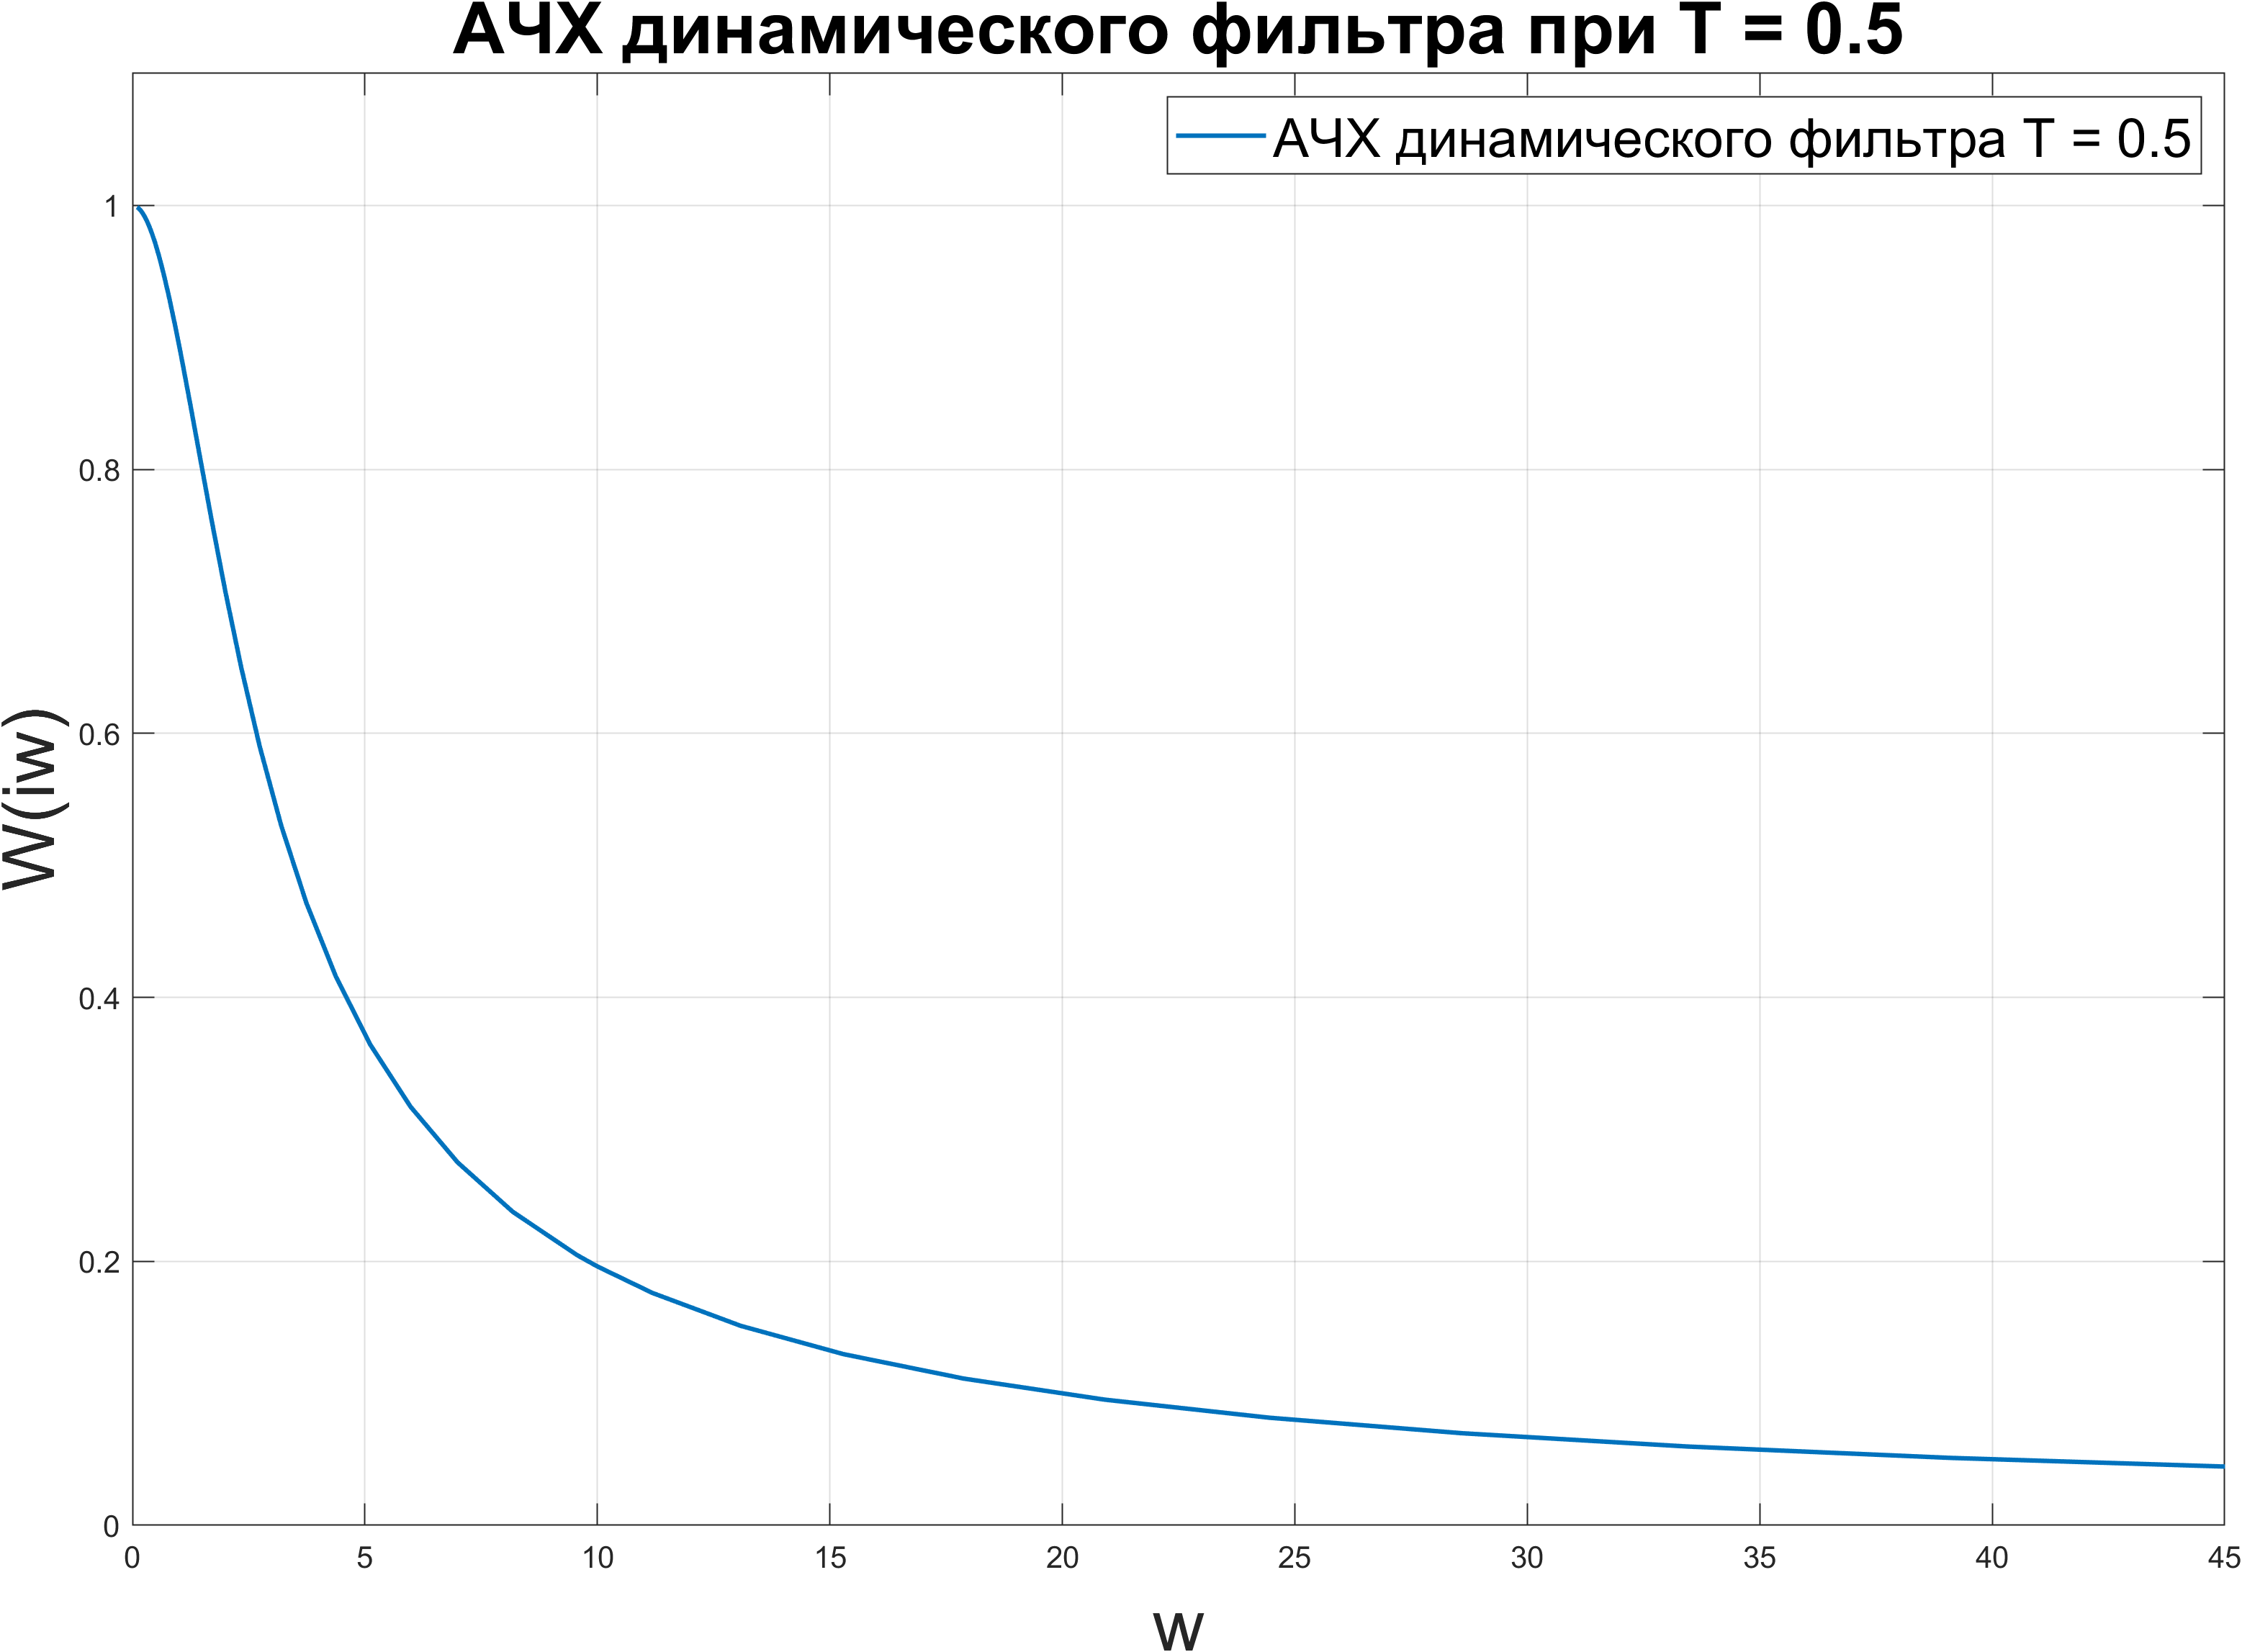
\includegraphics[width=0.92\textwidth, keepaspectratio]{images/filter_ach_T_0.5.png}
    \caption{АЧХ при $T = 0.5$}
\end{figure}
\begin{figure}[H]
    \centering
    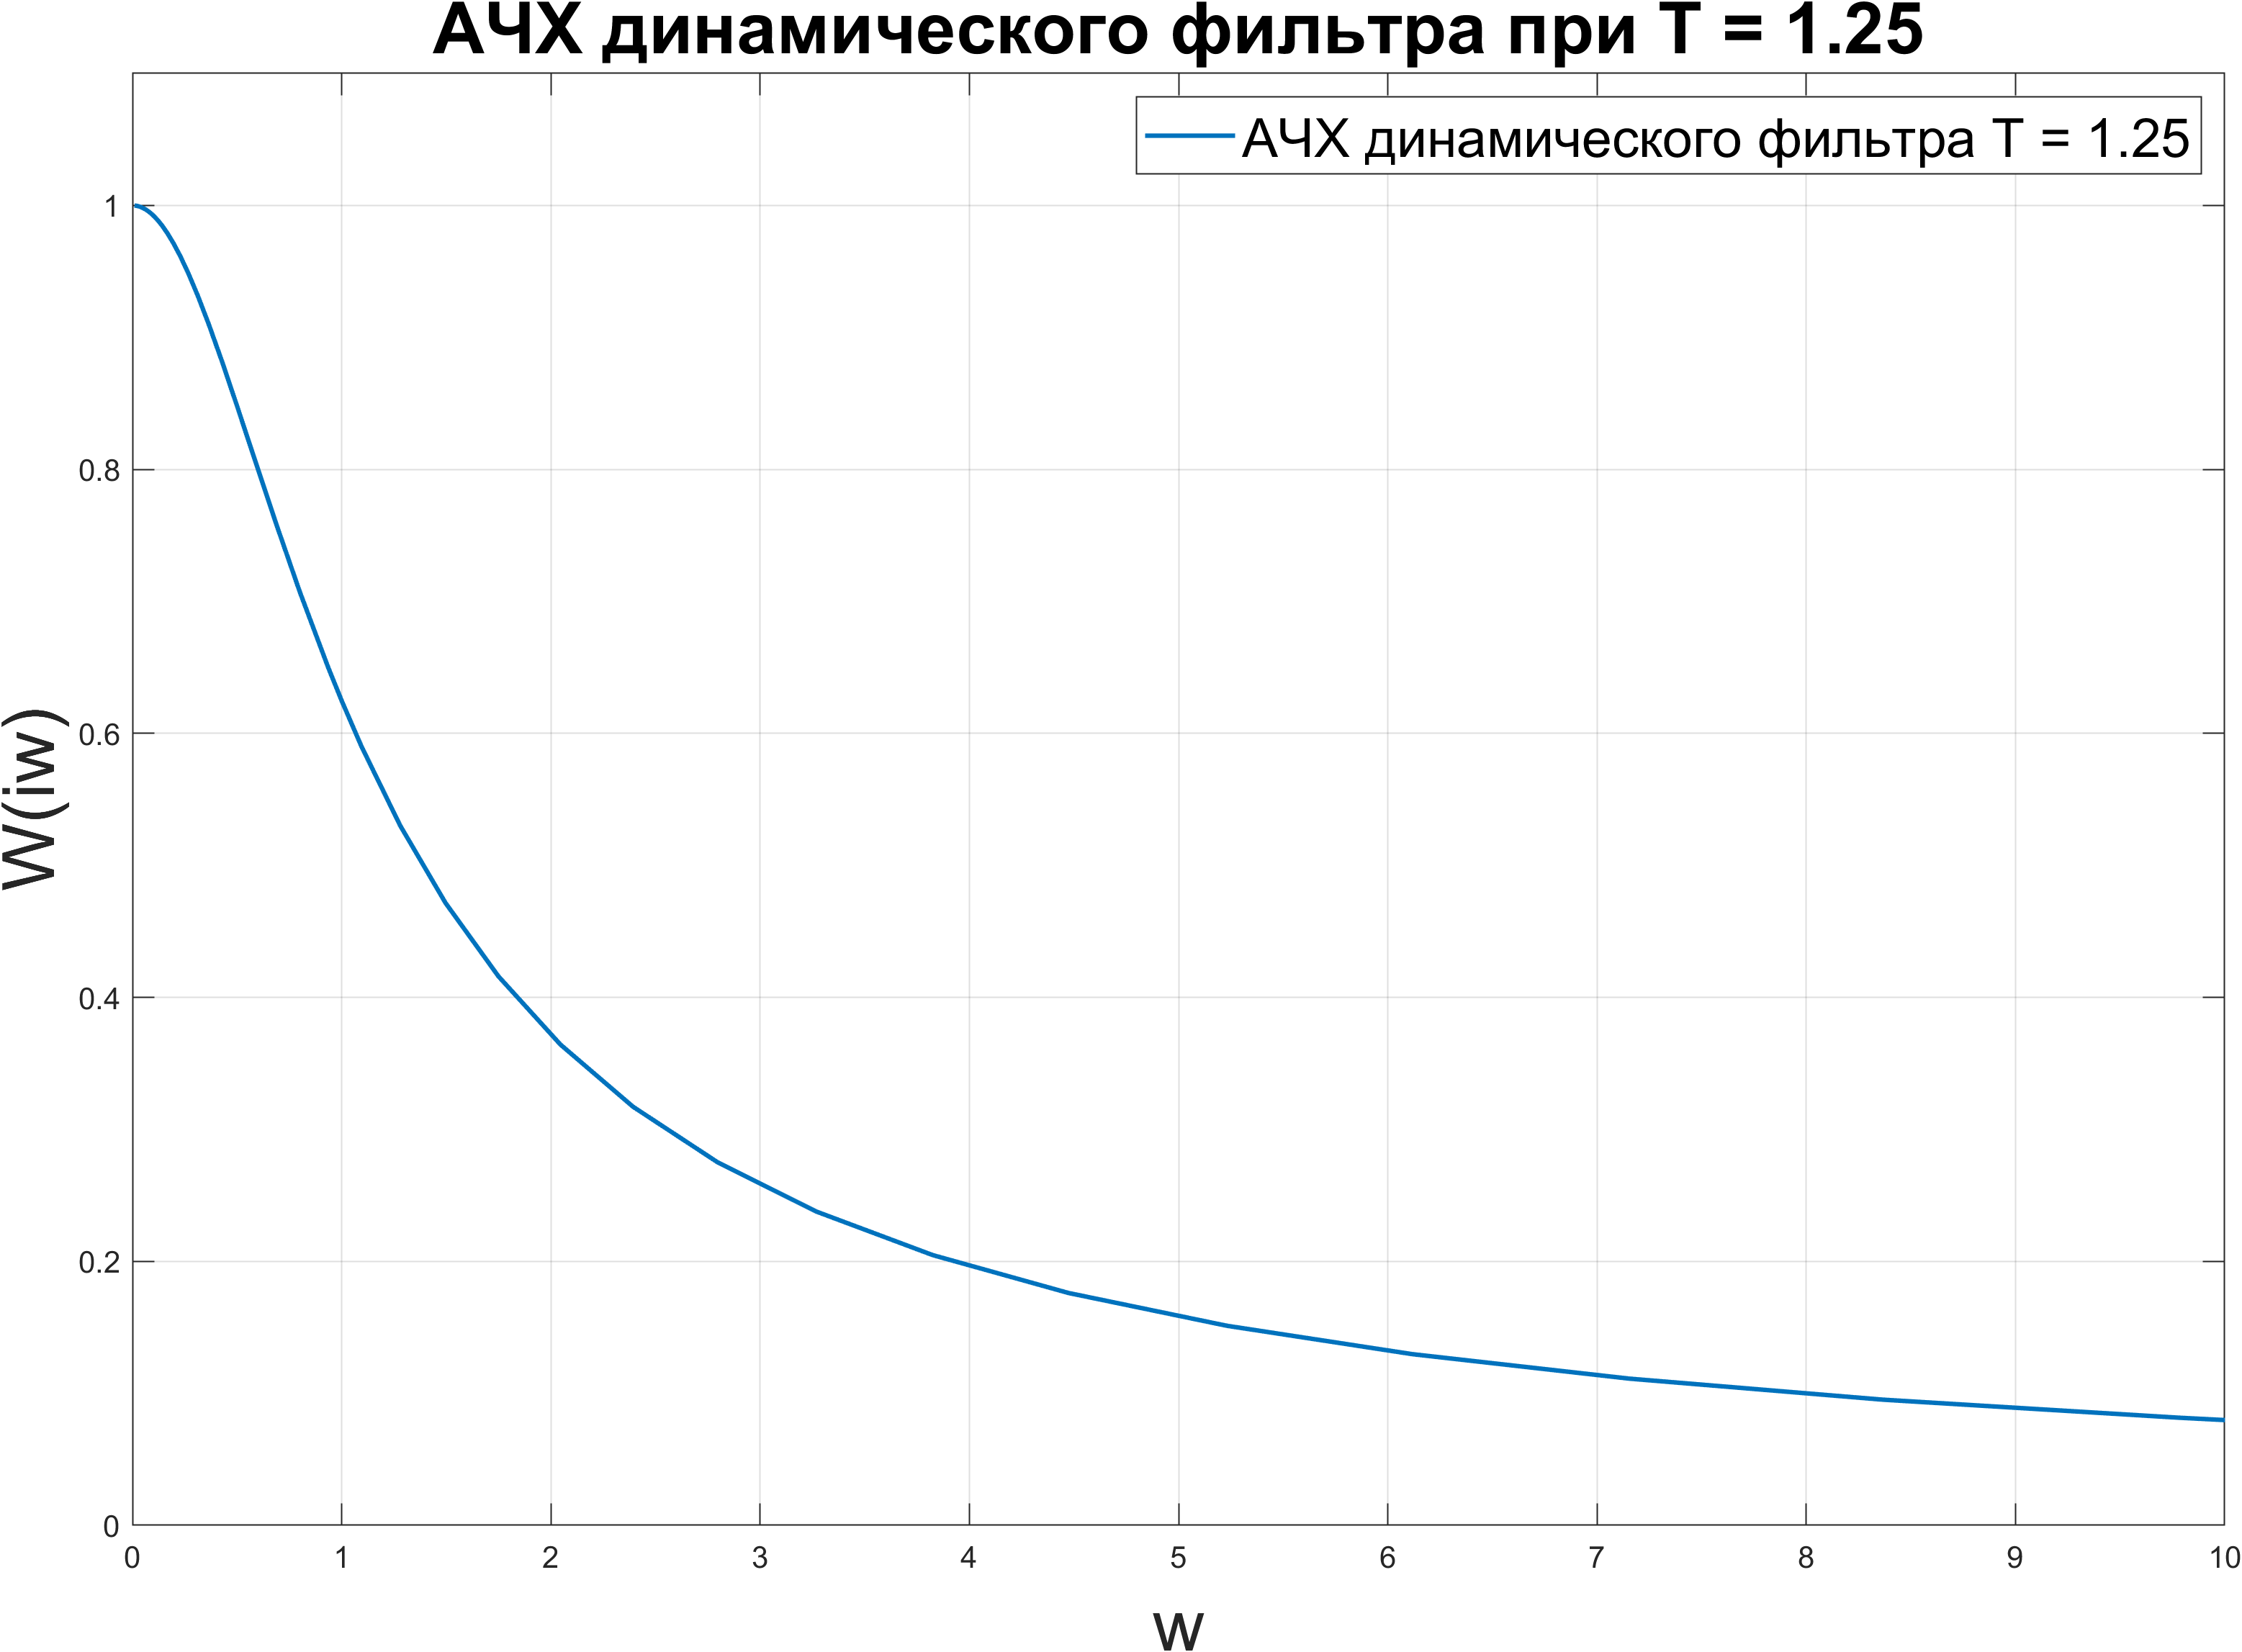
\includegraphics[width=0.92\textwidth, keepaspectratio]{images/filter_ach_T_1.25.png}
    \caption{АЧХ при $T = 1.5$}
\end{figure}
\newpage

\begin{figure}[H]
    \centering
    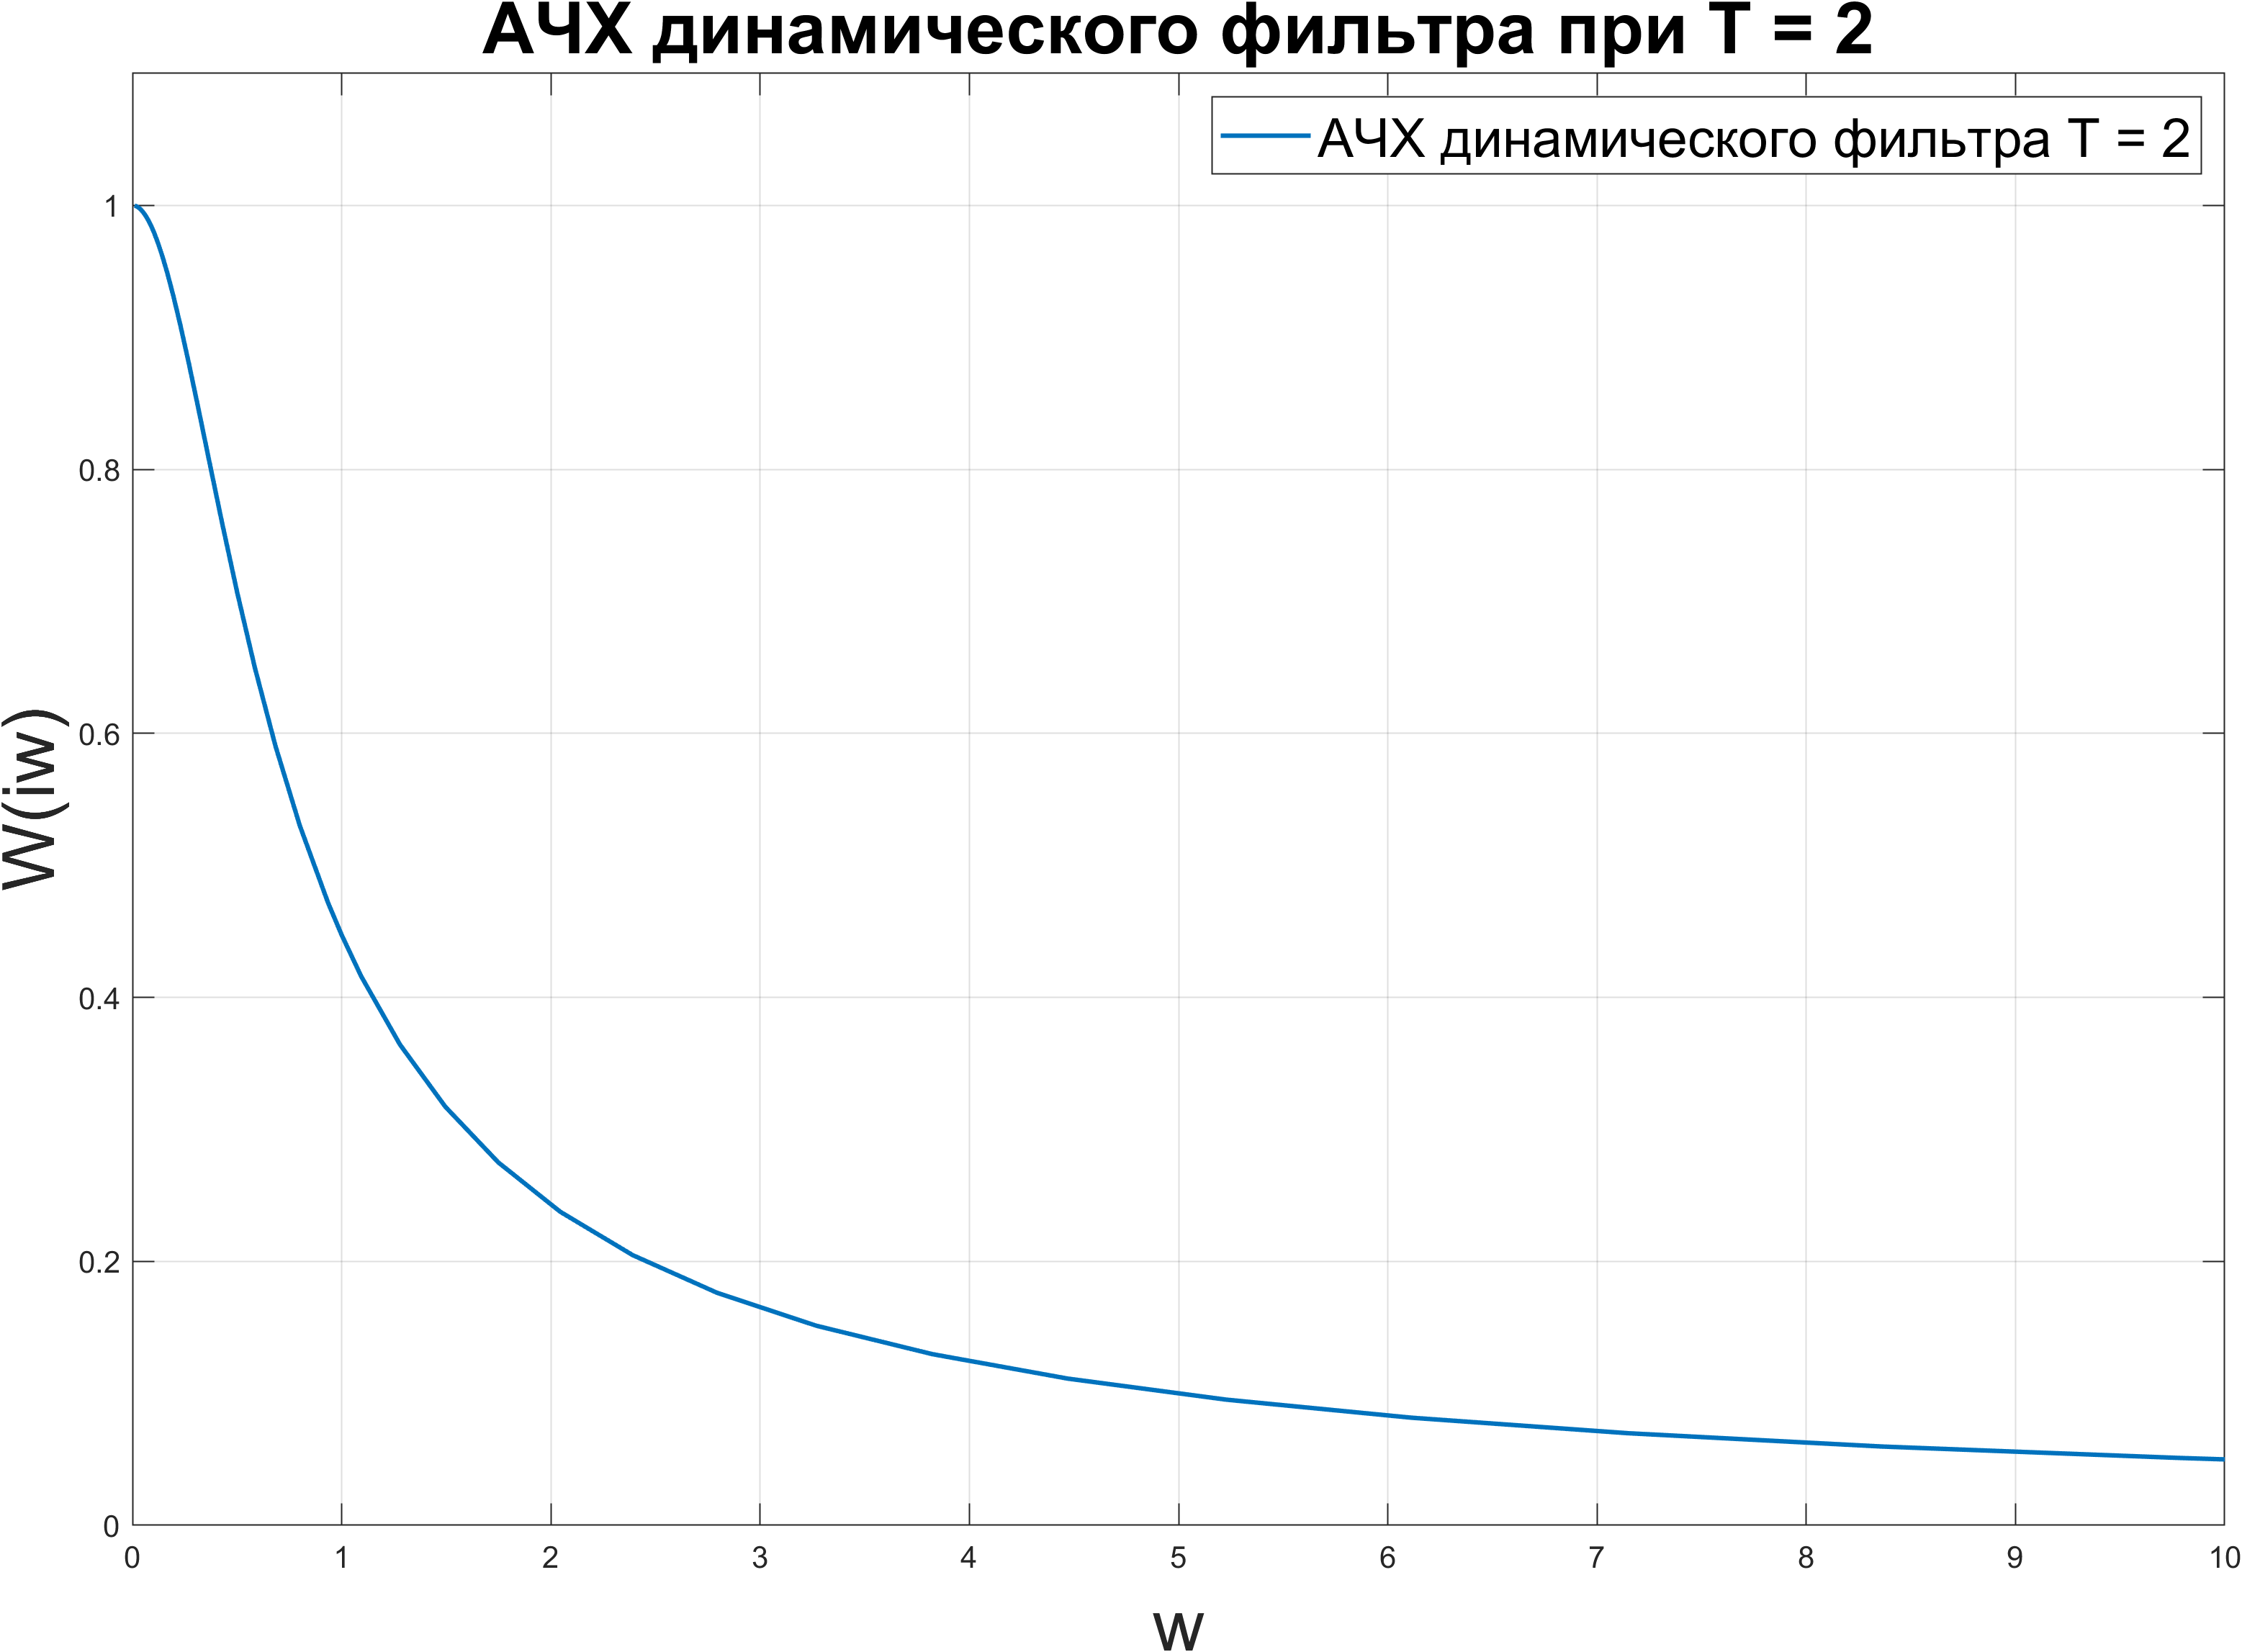
\includegraphics[width=0.92\textwidth, keepaspectratio]{images/filter_ach_T_2.png}
    \caption{АЧХ при $T = 2.0$}
\end{figure}
% ==========================================
% БЛОК 2: Фильтрация сигнала при разных T
% ==========================================
\subsection{Фильтрация сигнала (параметр $T$)}
При увеличении \(T\) сила фильтрации увеличивается, при значении \(0.1\) фильтр действует слишком слабо и шум почти не отфильтровался.
При значении порядка \(0.5\) фильтрованные значения близки к исходным, но шум остаётся.
При значении \(1.25\) шумы сильно сглажены, но начинает проявляться оклнение на правом конце квадратного импульса, в дальнейшем, при фиксированном \(T\) будет использоваться именно это значение.
При значении \(1.25\) шумы сильно сглажены в области вне импульса, где значения функции 0, но в области самого импульса получается очень пологий график, никак не соответствующий исходному.
\newpage
\begin{figure}[H]
    \centering
    
\includegraphics[width=0.92\textwidth, keepaspectratio]{images/filter_T_0.1.png}
    \caption{Фильтрация при $T = 0.1$}
\end{figure}
\begin{figure}[H]
    \centering
    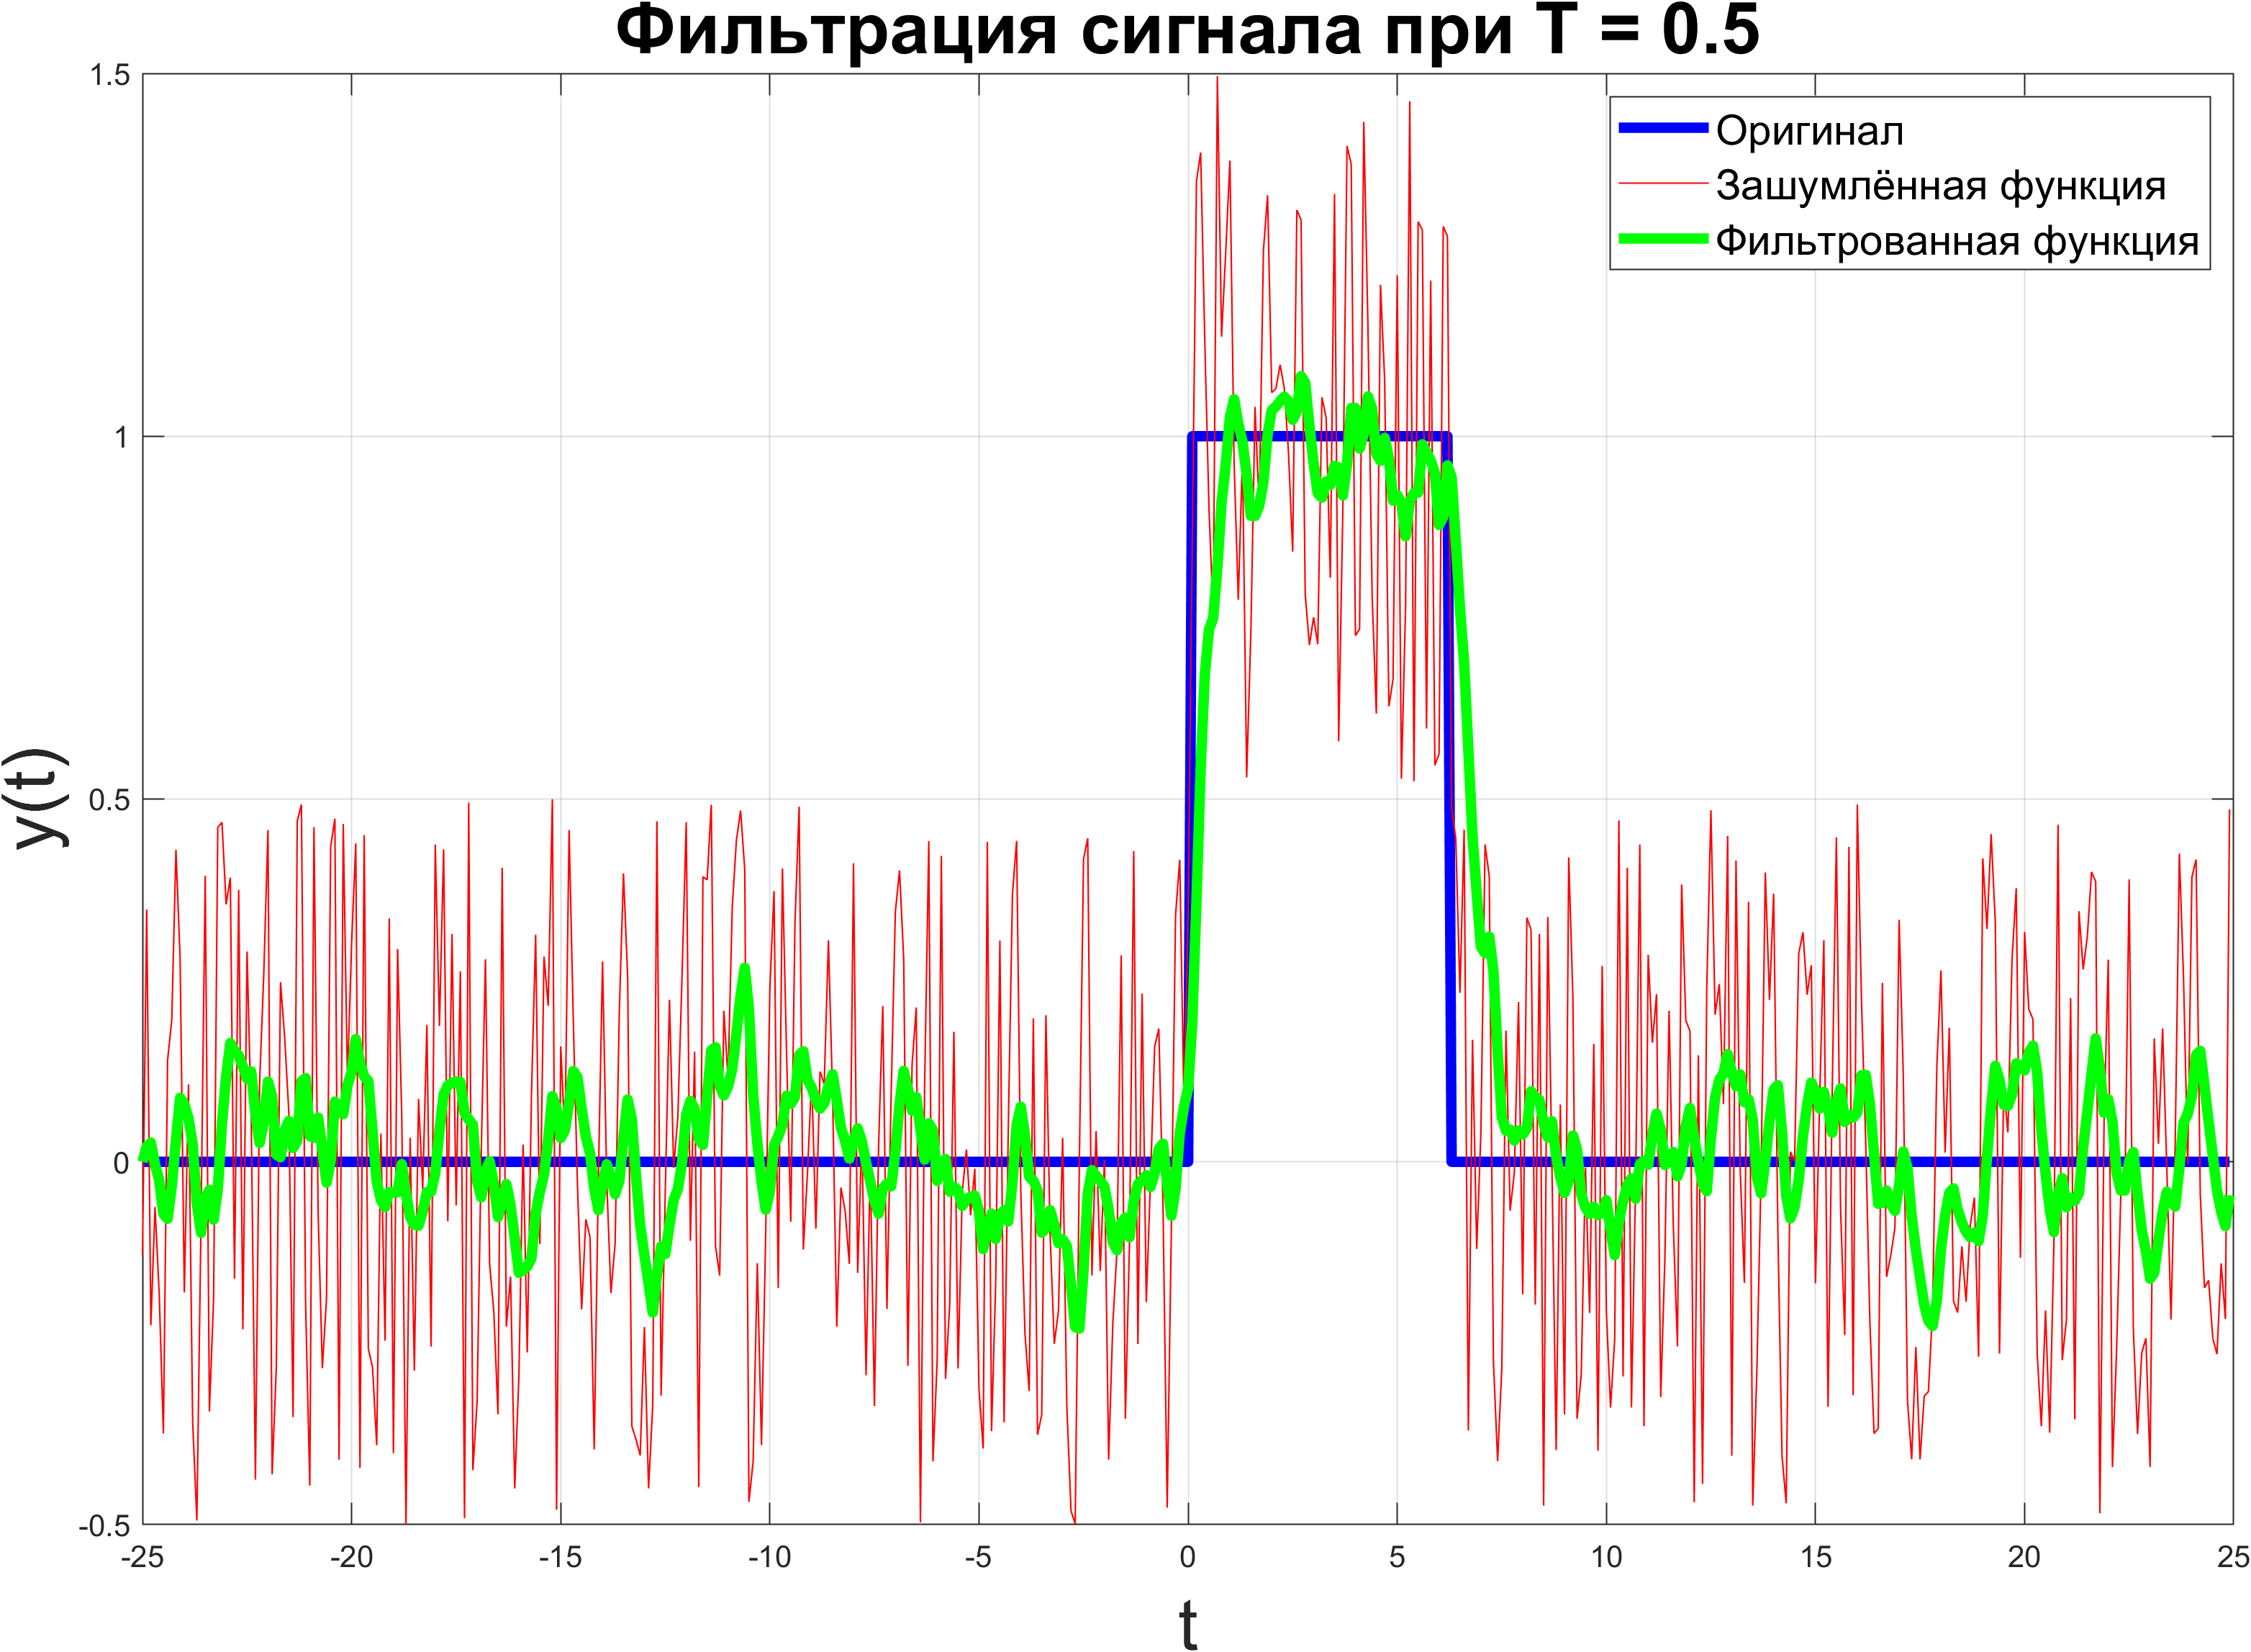
\includegraphics[width=0.92\textwidth, keepaspectratio]{images/filter_T_0.5.png}
    \caption{Фильтрация при $T = 0.5$}
\end{figure}
\newpage

\begin{figure}[H]
    \centering
    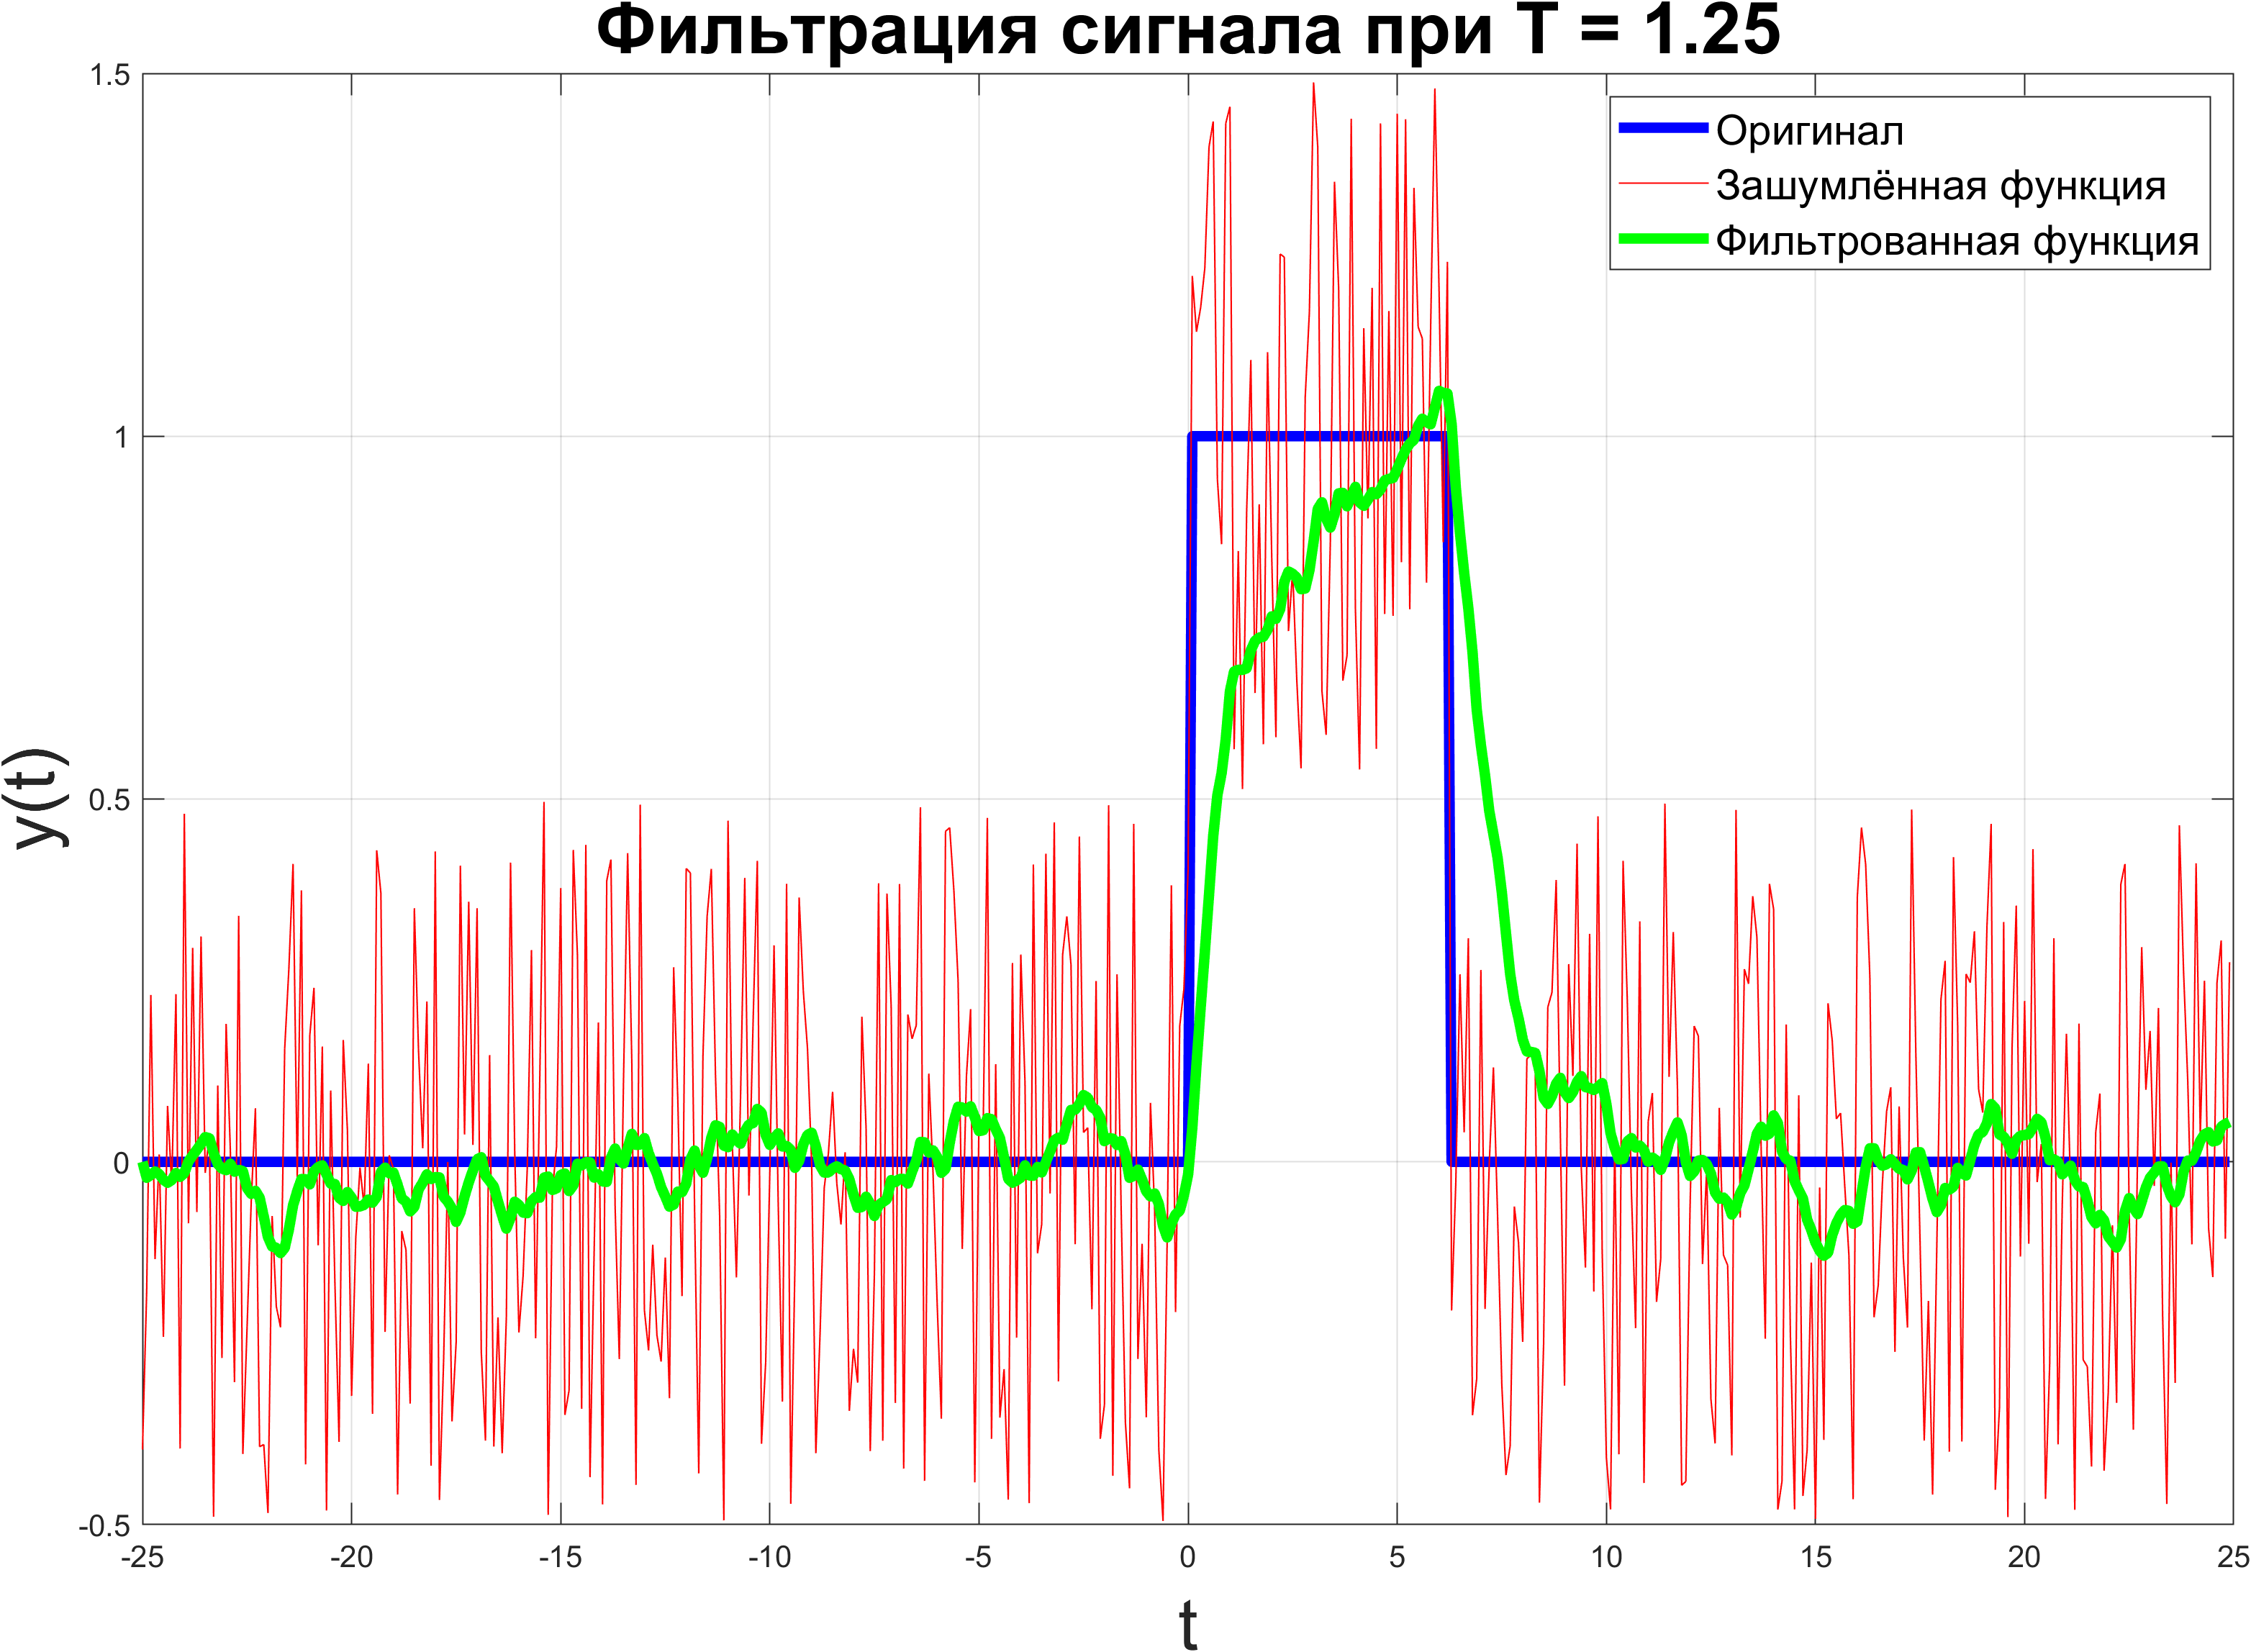
\includegraphics[width=0.92\textwidth, keepaspectratio]{images/filter_T_1.25.png}
    \caption{Фильтрация при $T = 1.5$}
\end{figure}
\begin{figure}[H]
    \centering
    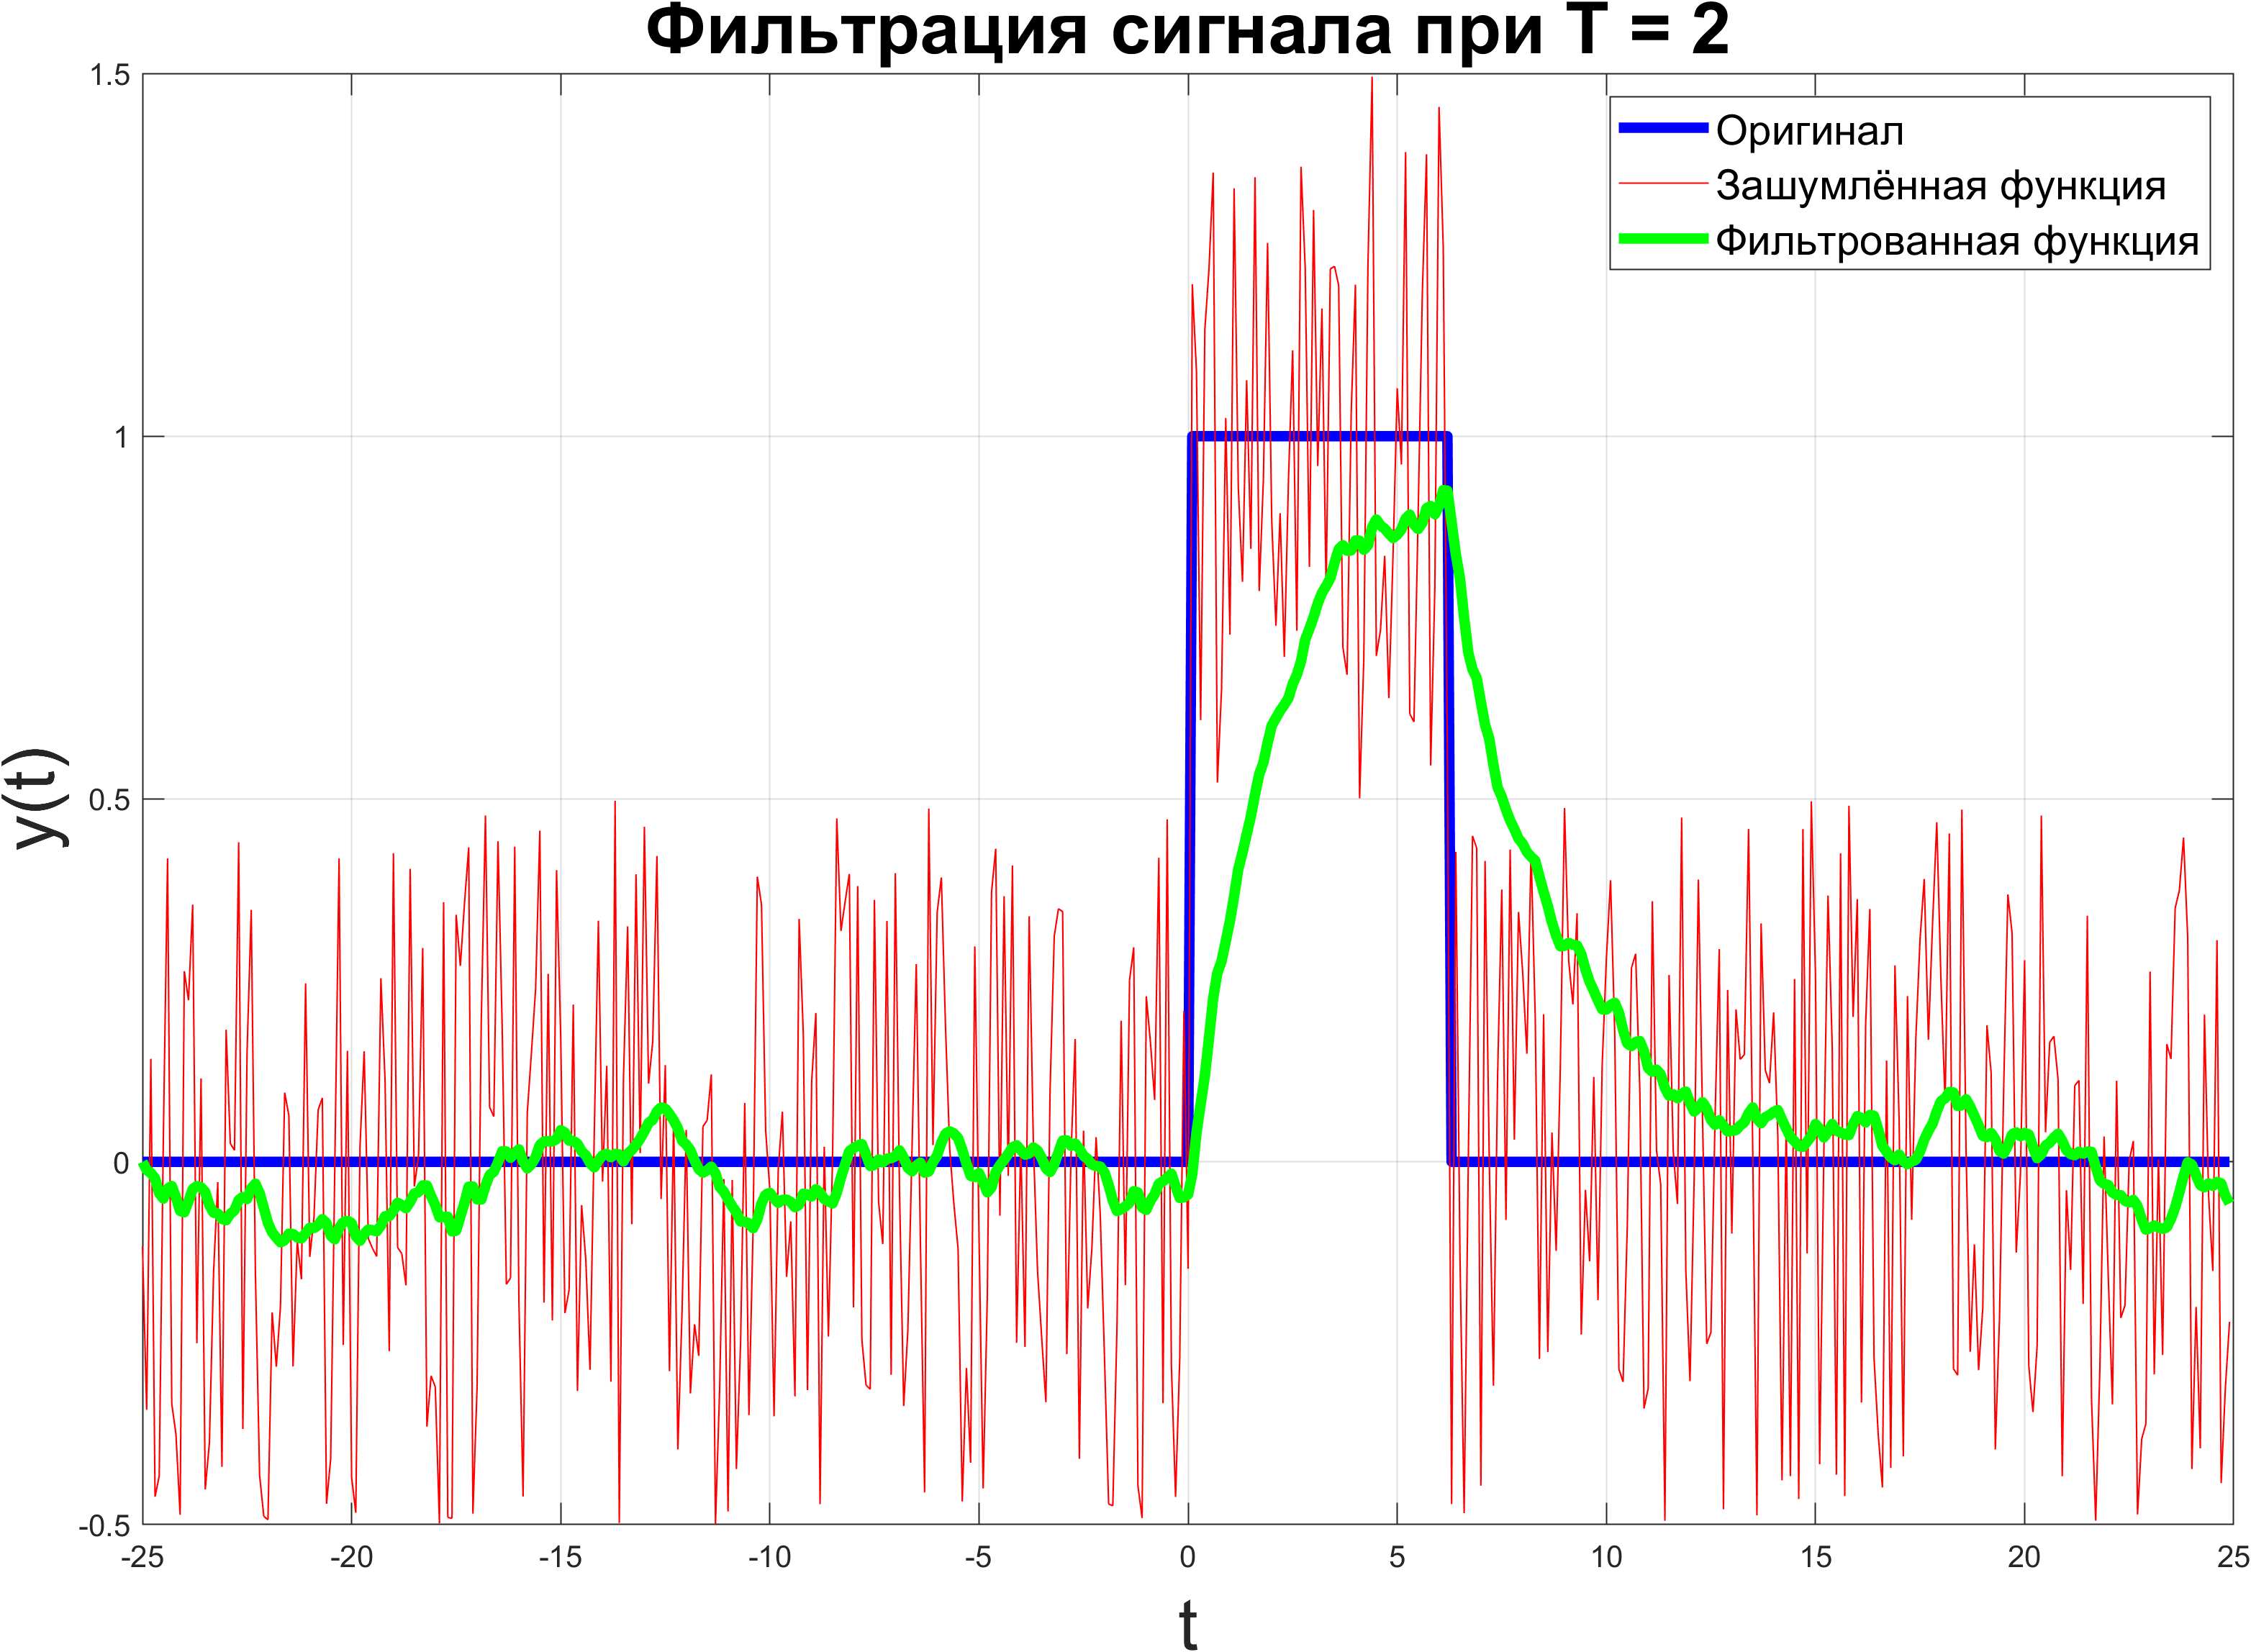
\includegraphics[width=0.92\textwidth, keepaspectratio]{images/filter_T_2.png}
    \caption{Фильтрация при $T = 2.0$}
\end{figure}
\newpage
% ==========================================
% БЛОК 3: Сравнение методов при разных T
% ==========================================
\subsection{Сравнение методов фильтрации (параметр $T$)}
На данных графиках видно, что функция, полученнная обратным преобразованием от произведения передаточной функции на Фурье-образ зашумлённого сигнала отличается в пределах погрешности методов.

\begin{figure}[H]
    \centering
    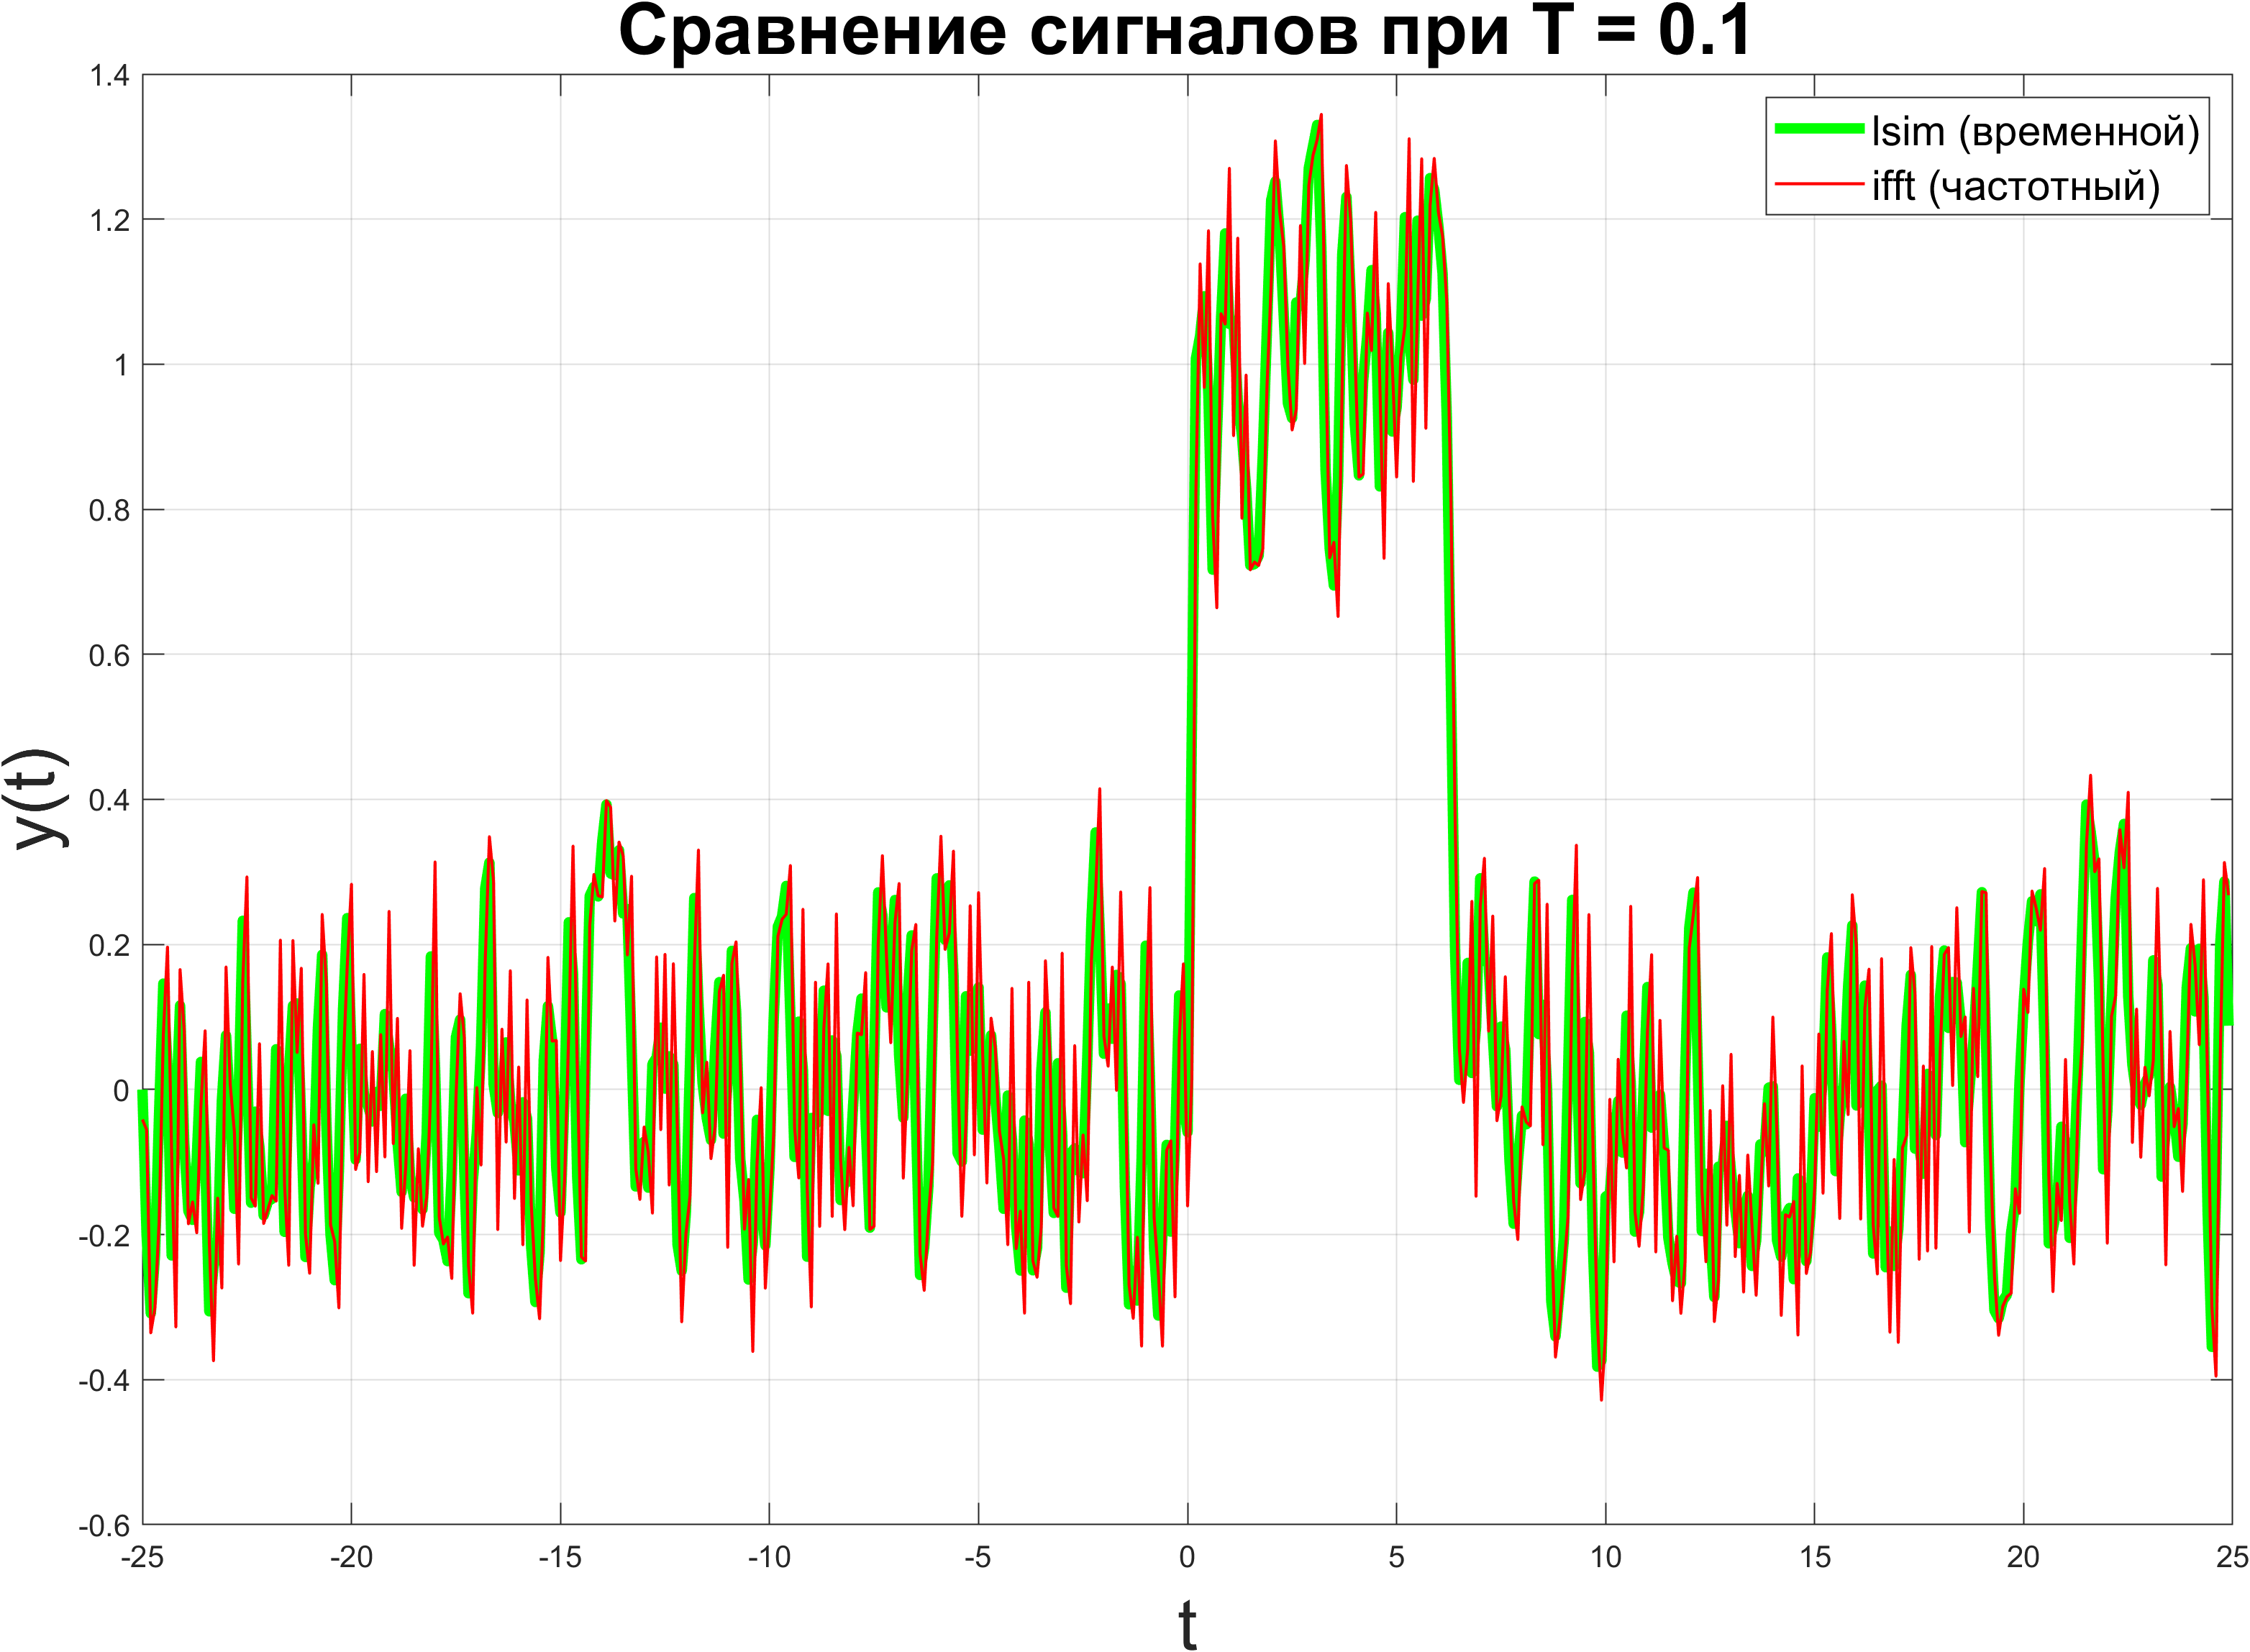
\includegraphics[width=0.80\textwidth, keepaspectratio]{images/filter_transf_T_0.1.png}
    \caption{Сравнение методов при $T = 0.1$}
\end{figure}
\begin{figure}[H]
    \centering
    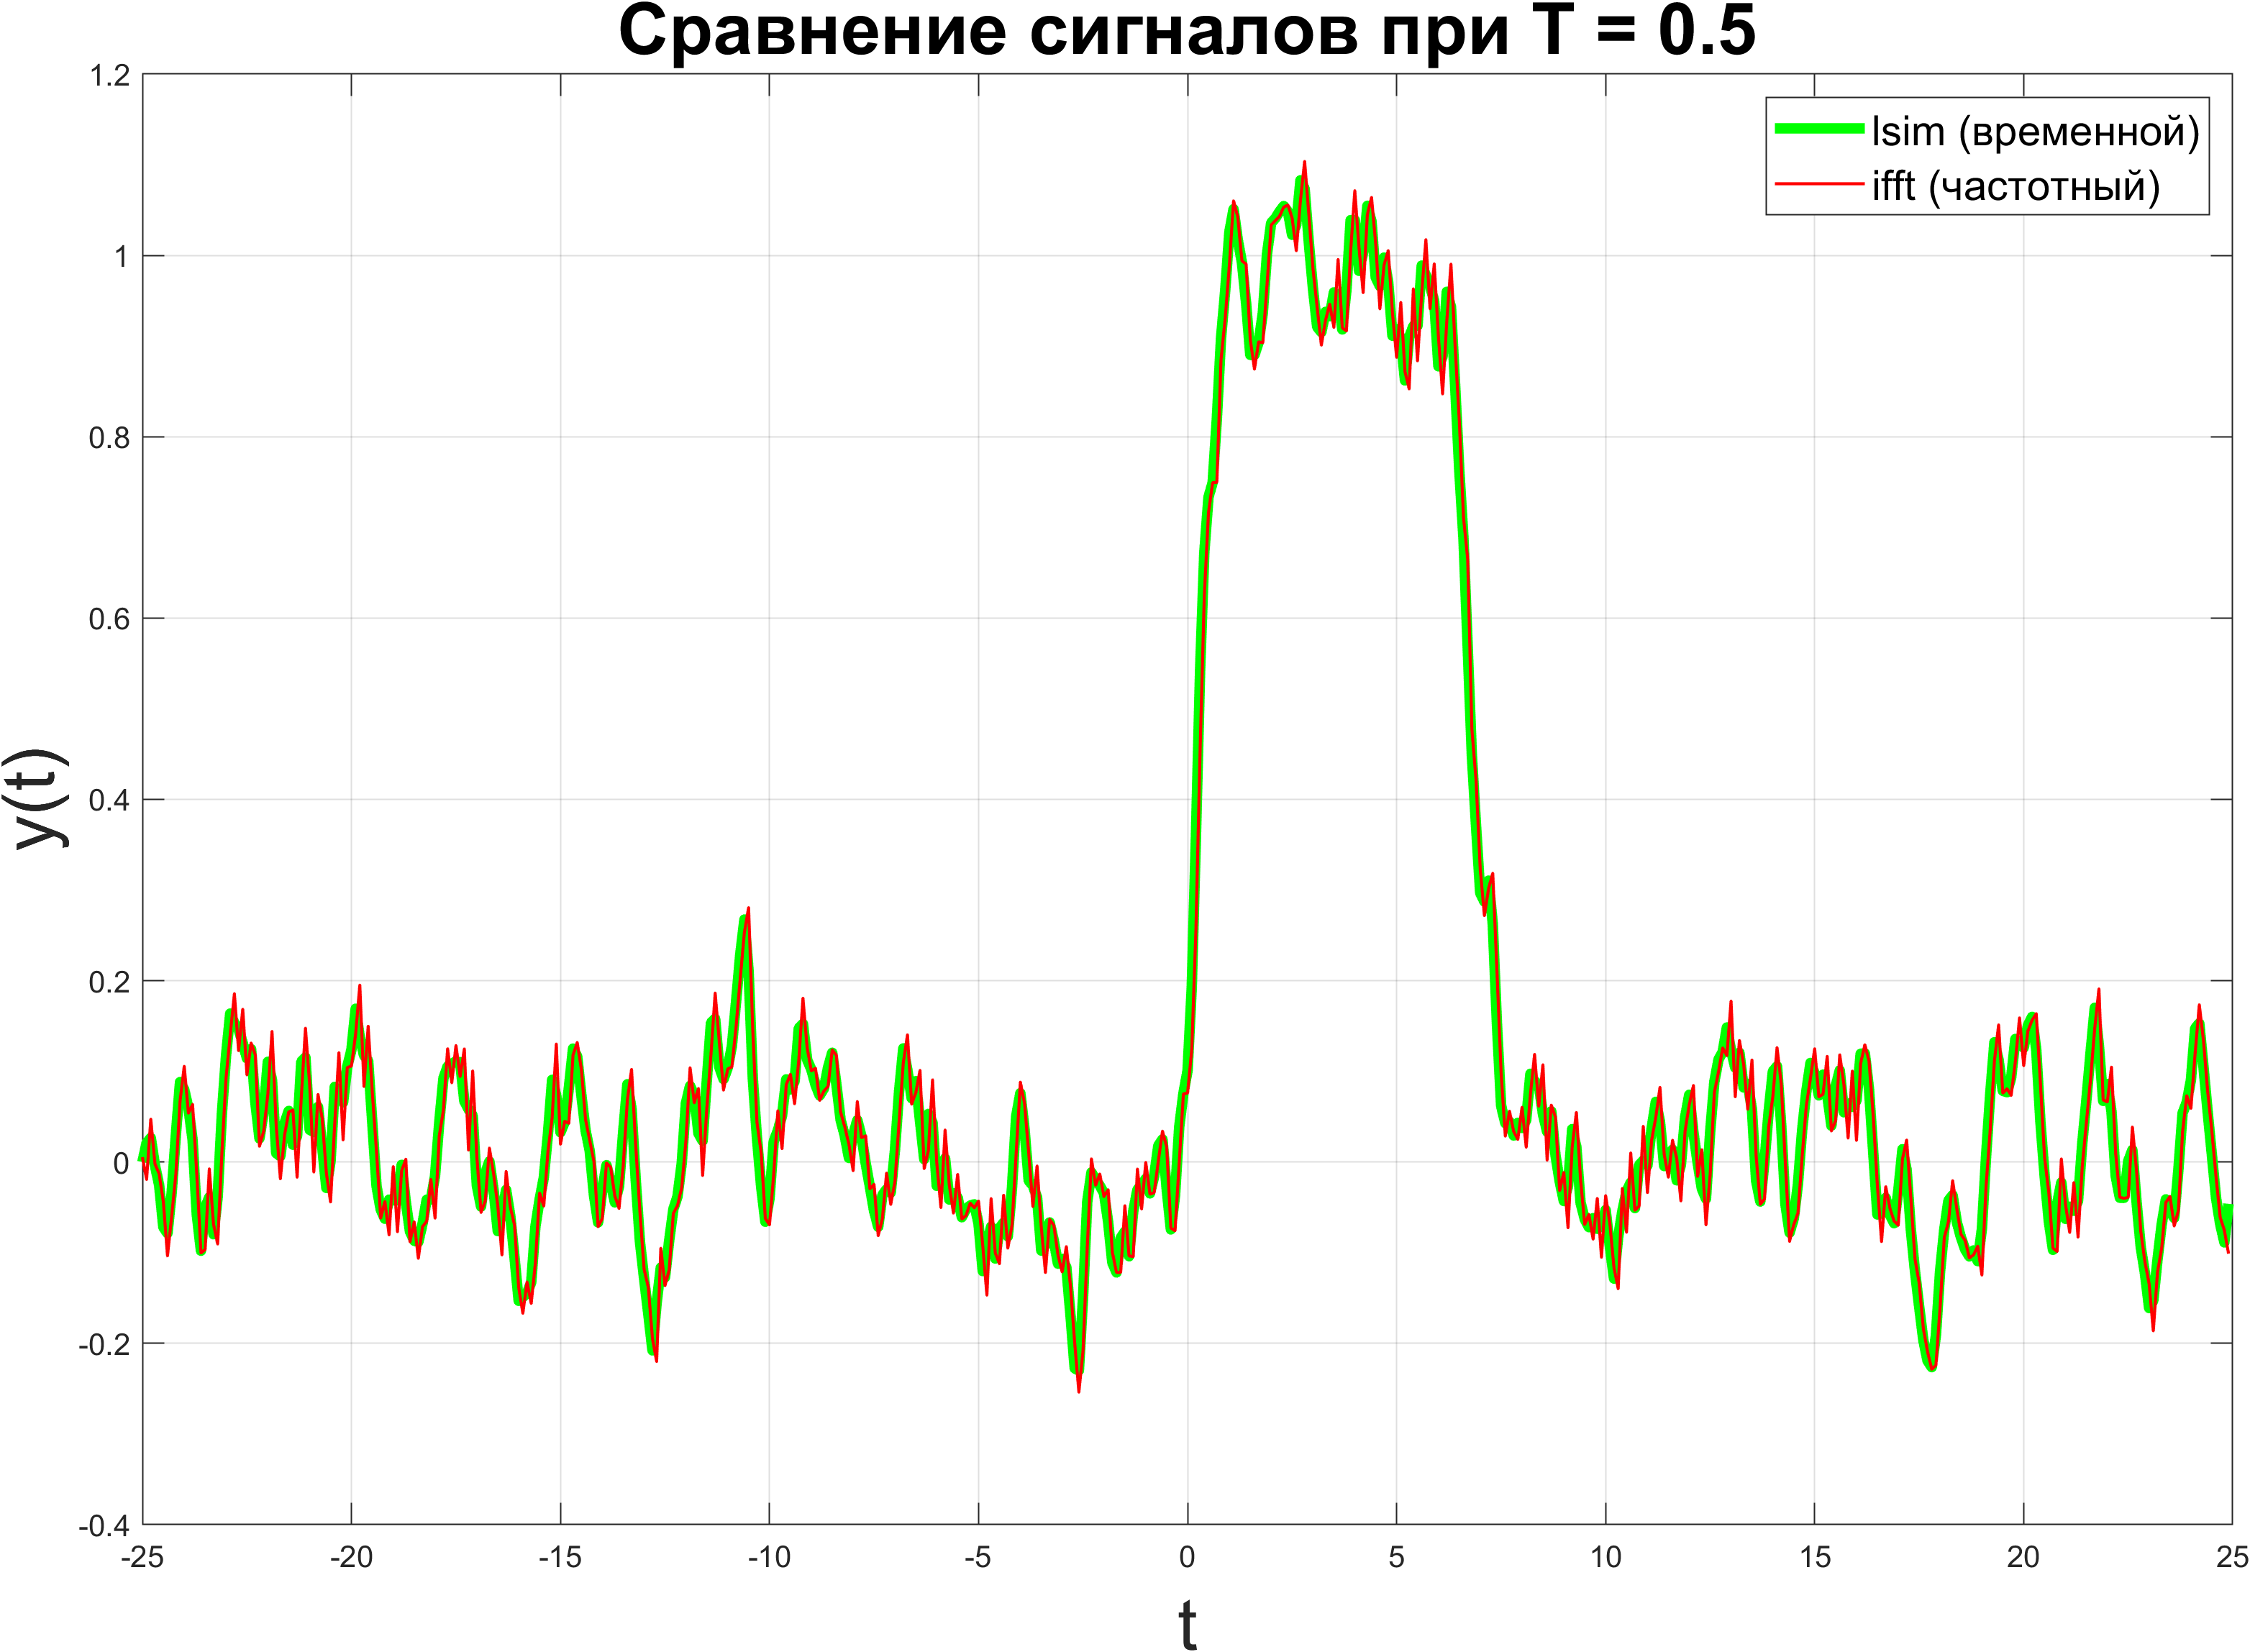
\includegraphics[width=0.80\textwidth, keepaspectratio]{images/filter_transf_T_0.5.png}
    \caption{Сравнение методов при $T = 0.5$}
\end{figure}
\newpage

\begin{figure}[H]
    \centering
    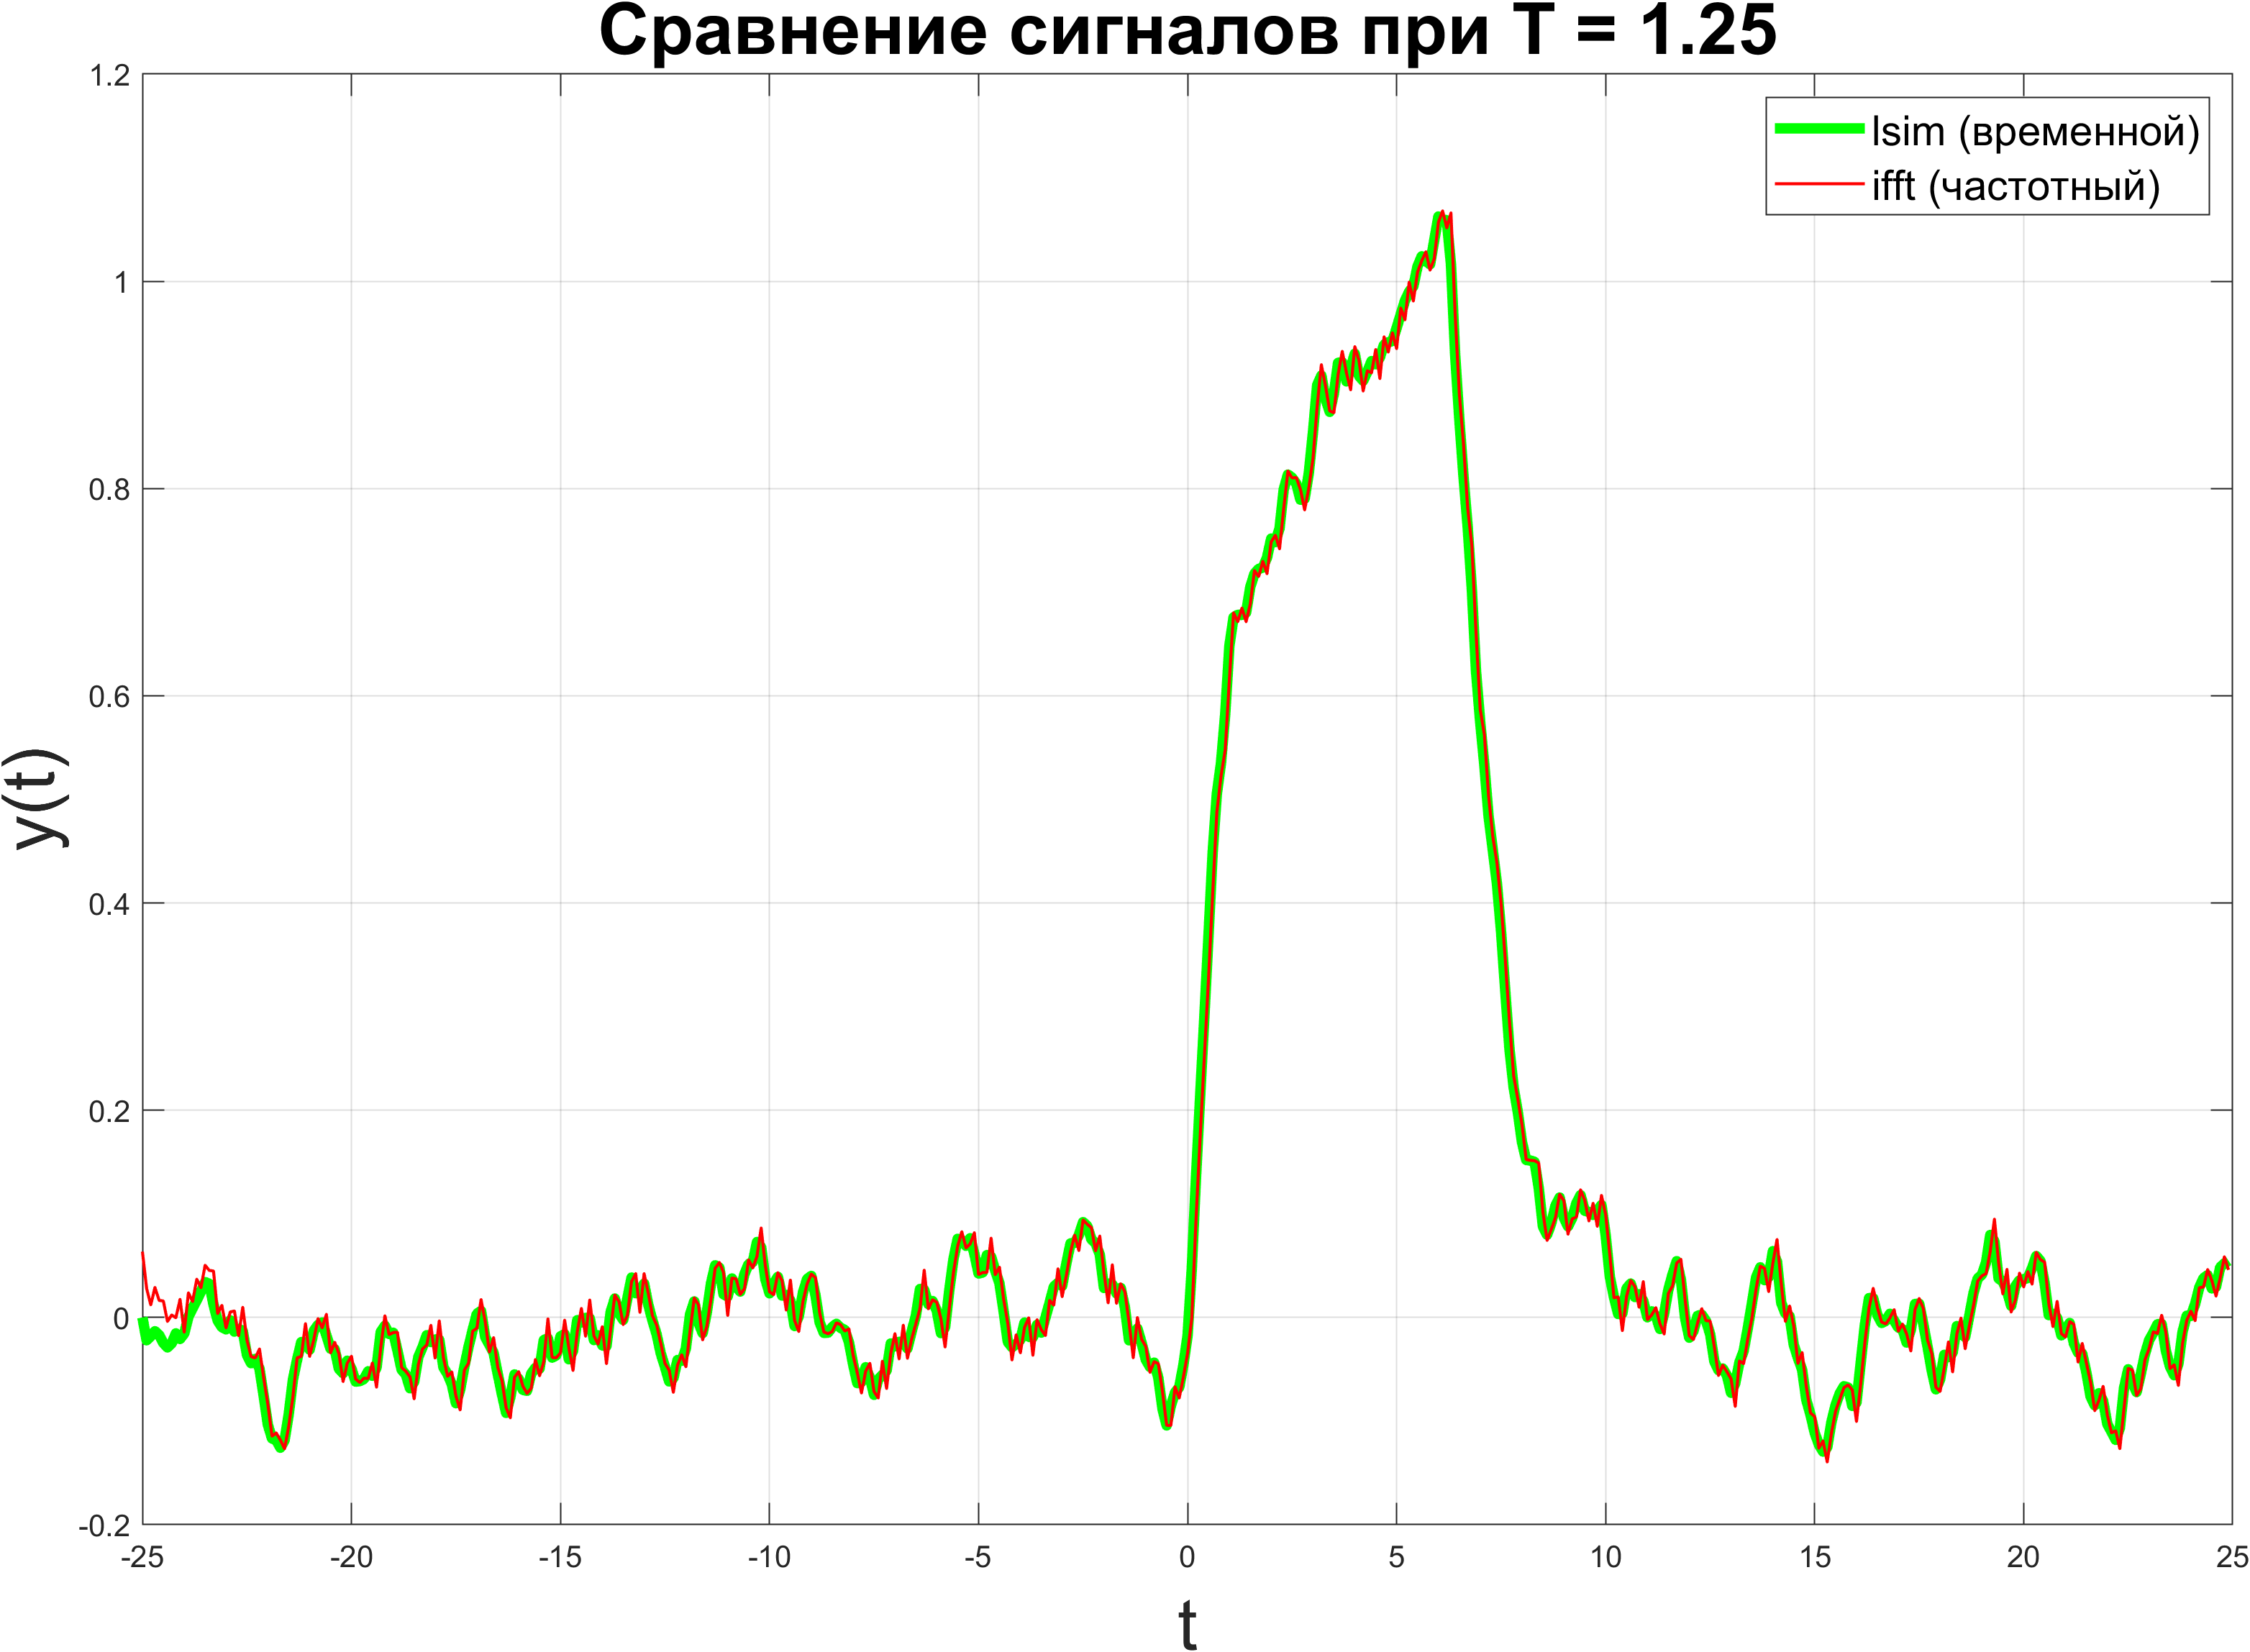
\includegraphics[width=0.92\textwidth, keepaspectratio]{images/filter_transf_T_1.25.png}
    \caption{Сравнение методов при $T = 1.5$}
\end{figure}
\begin{figure}[H]
    \centering
    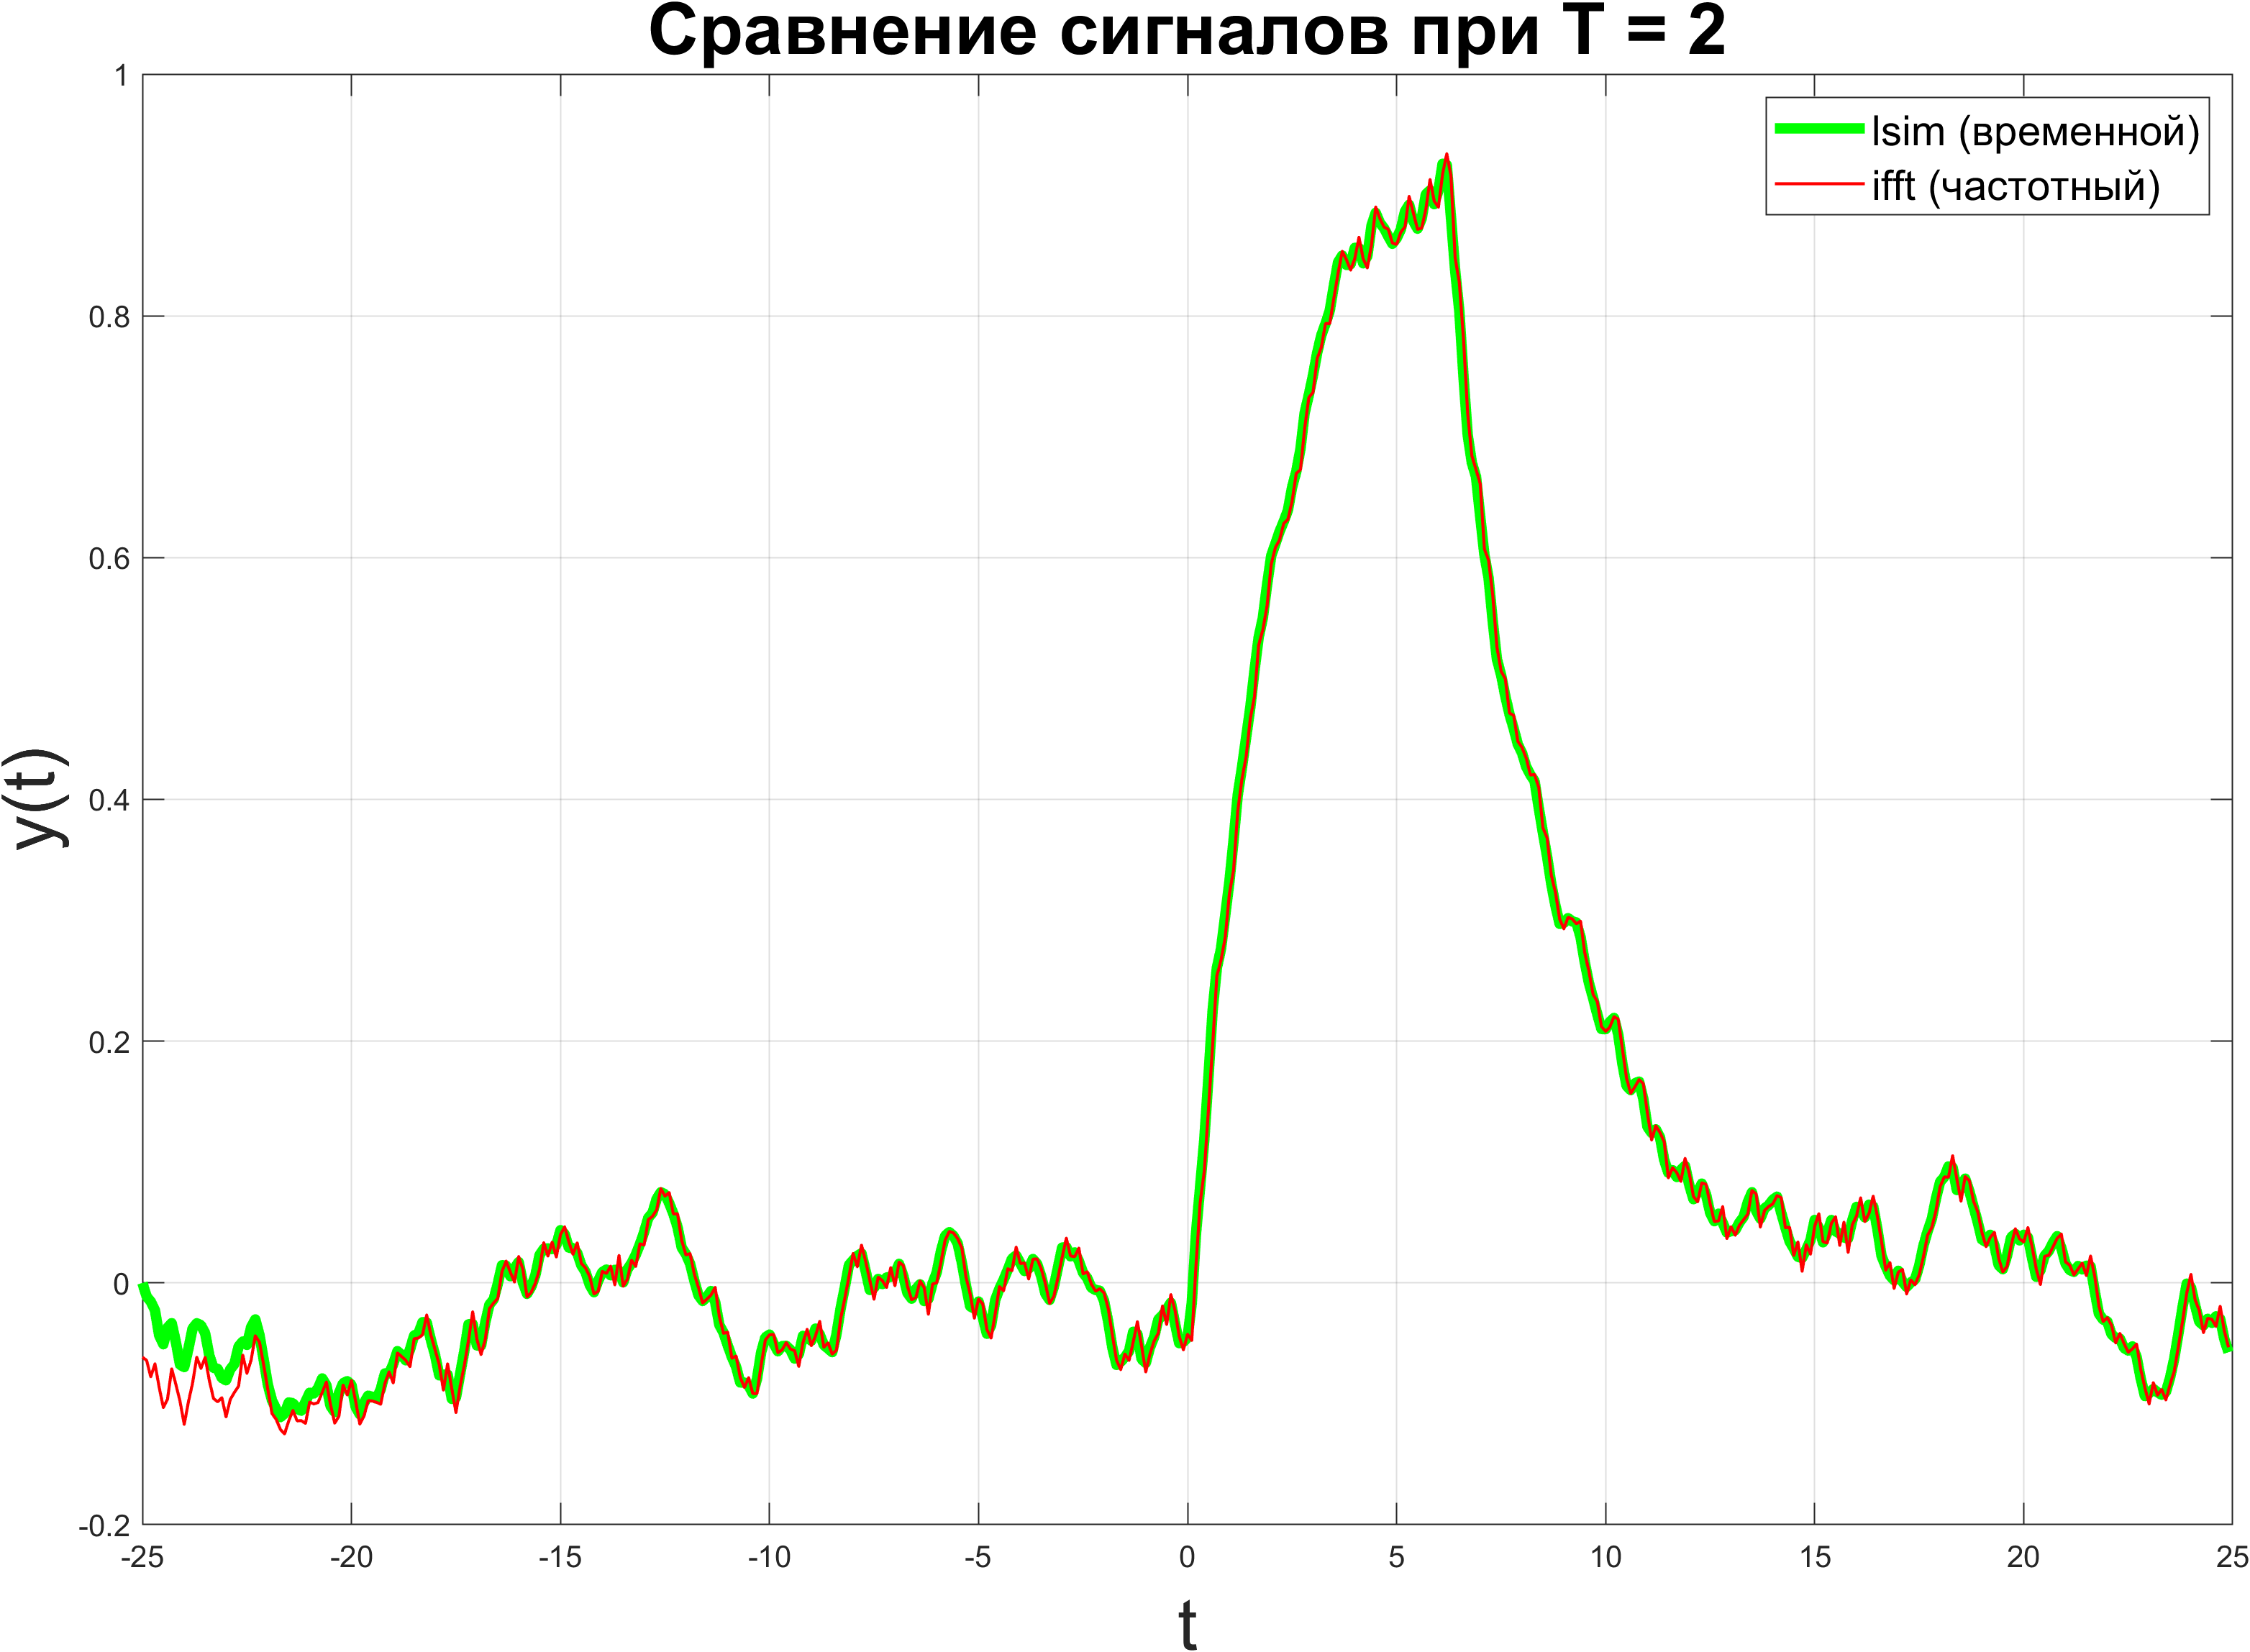
\includegraphics[width=0.92\textwidth, keepaspectratio]{images/filter_transf_T_2.png}
    \caption{Сравнение методов при $T = 2.0$}
\end{figure}
\newpage
% ==========================================
% БЛОК 4: Фурье-образы (сигналы) при разных T
% ==========================================
\subsection{Фурье-образы $g$, $y$, $y_{fil}$ (параметр $T$)}
При увеличении \(T\) Фурье-образ фильтрованной функции сохраняет значения ближе к нулю, но обнуляет остальные значения образа.

\begin{figure}[H]
    \centering
    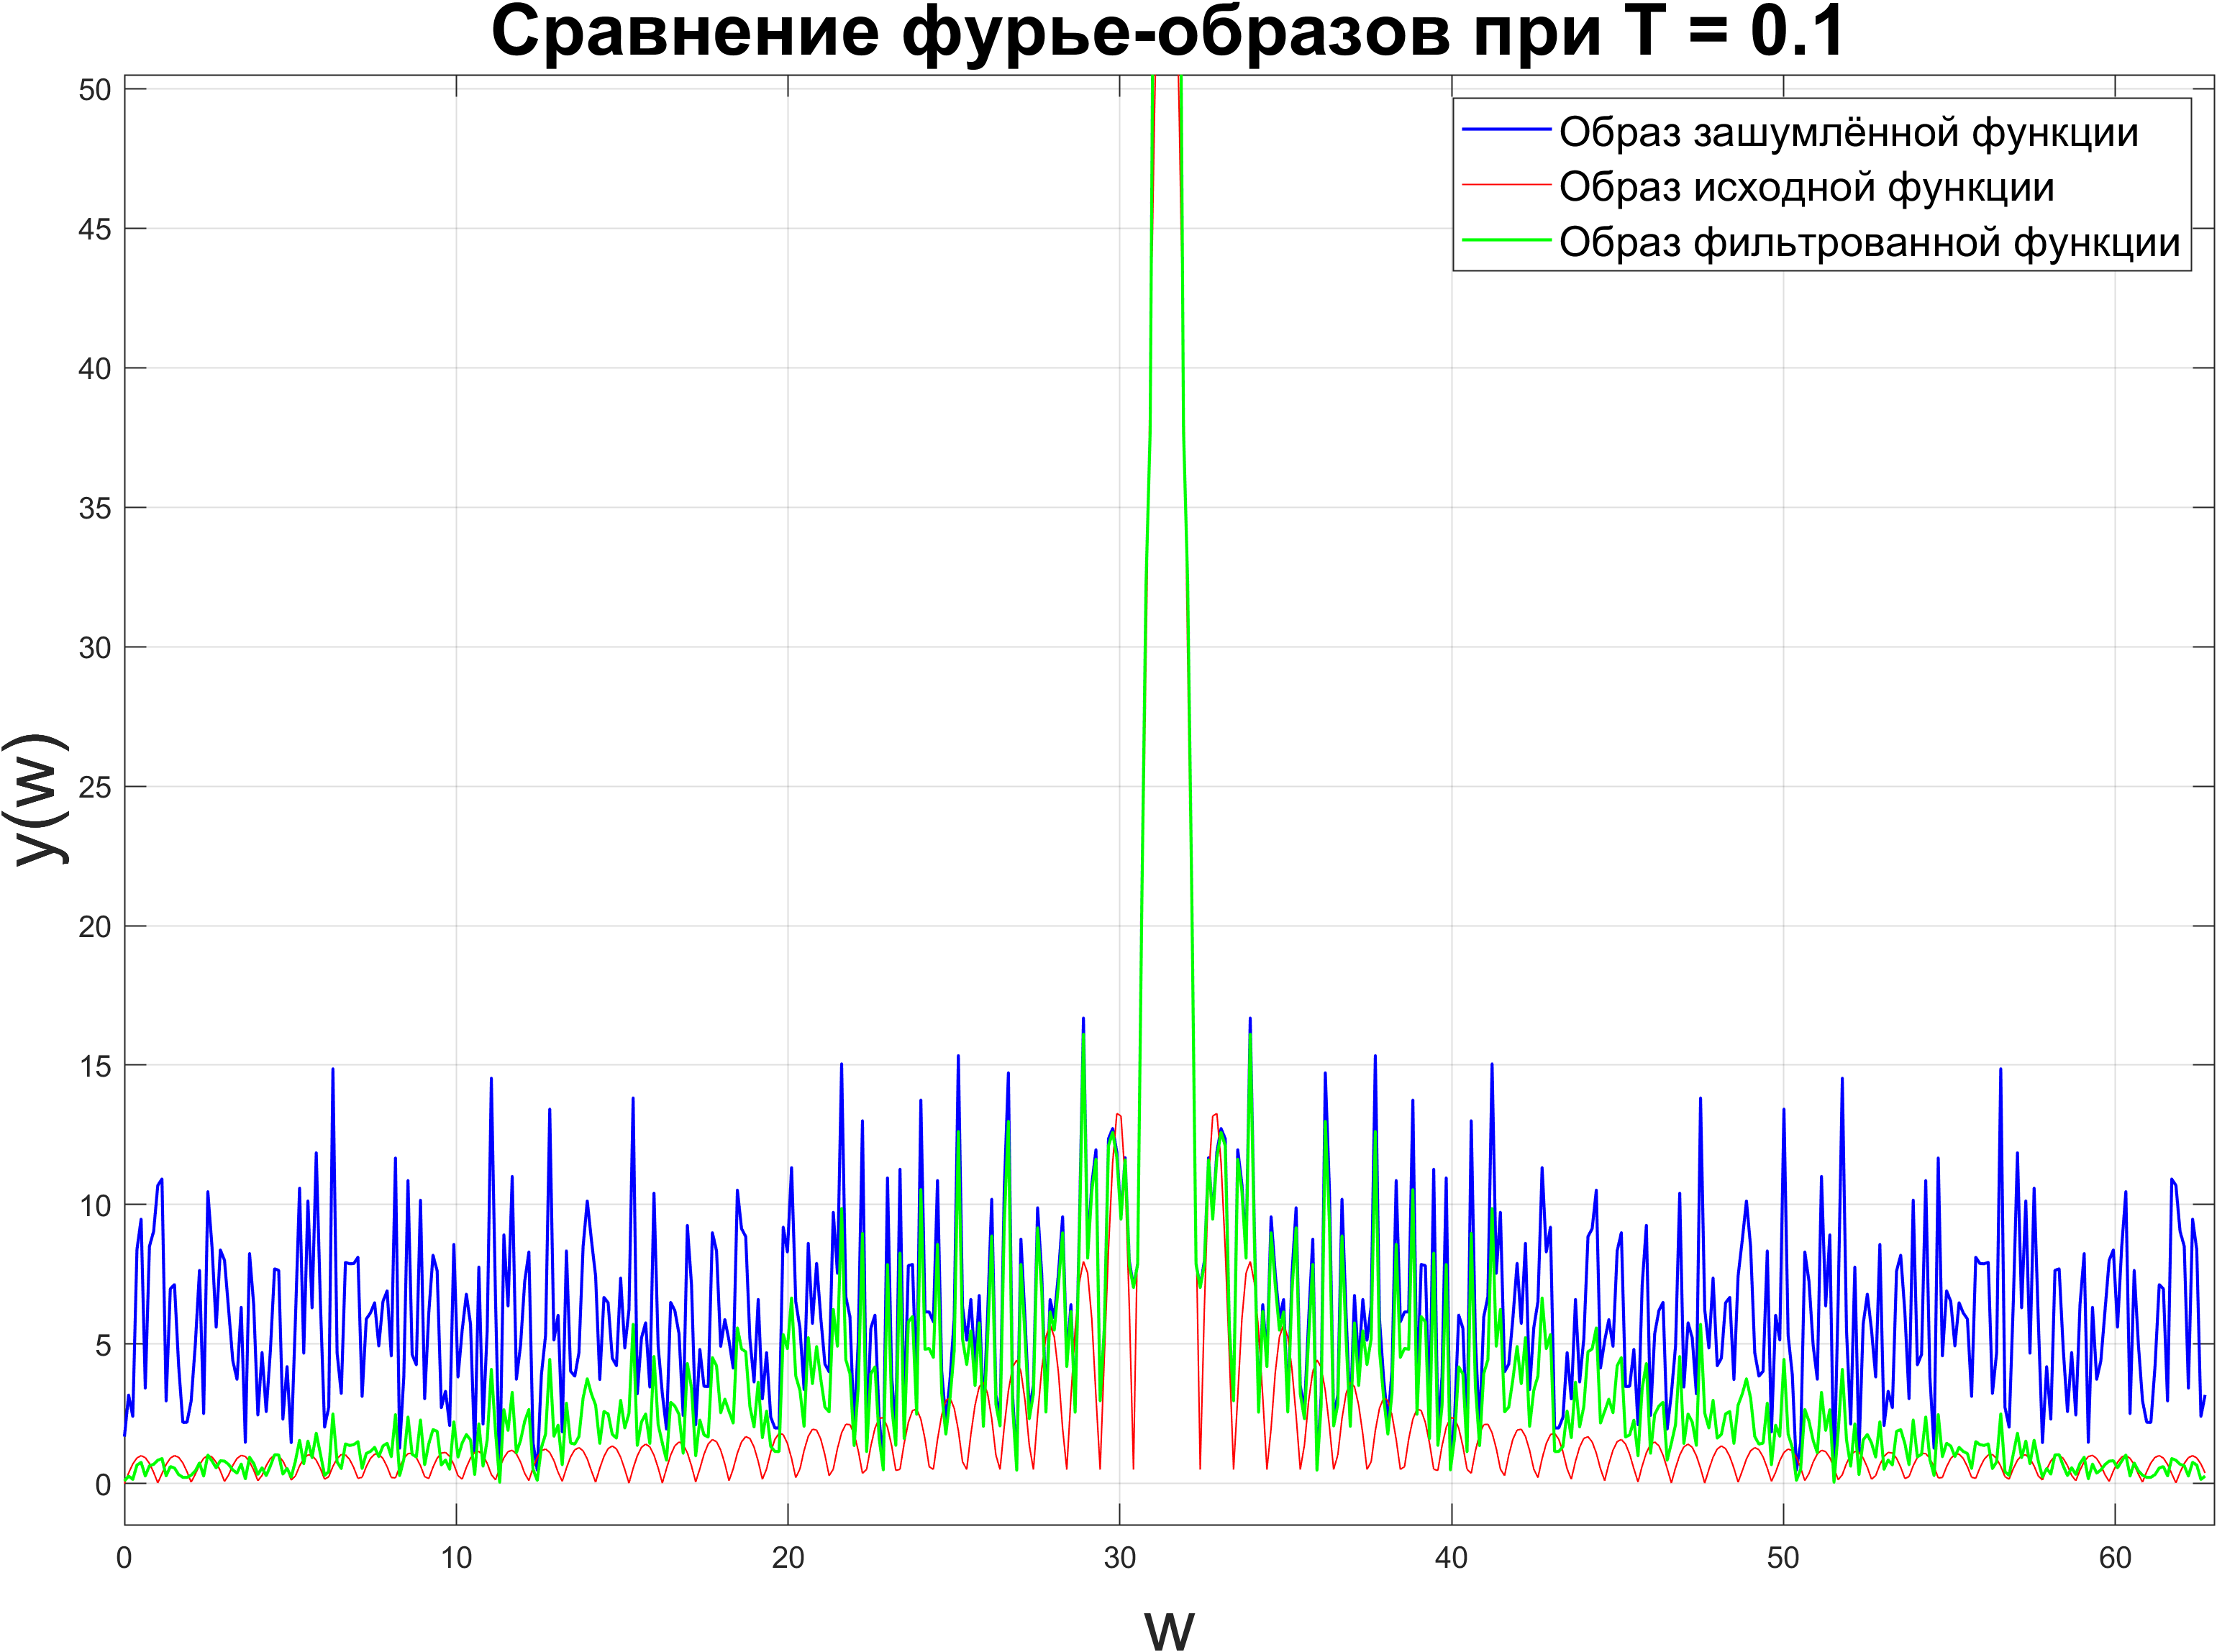
\includegraphics[width=0.80\textwidth, keepaspectratio]{images/fur_imgs_g_T_0.1.png}
    \caption{Фурье-образы при $T = 0.1$}
\end{figure}
\begin{figure}[H]
    \centering
    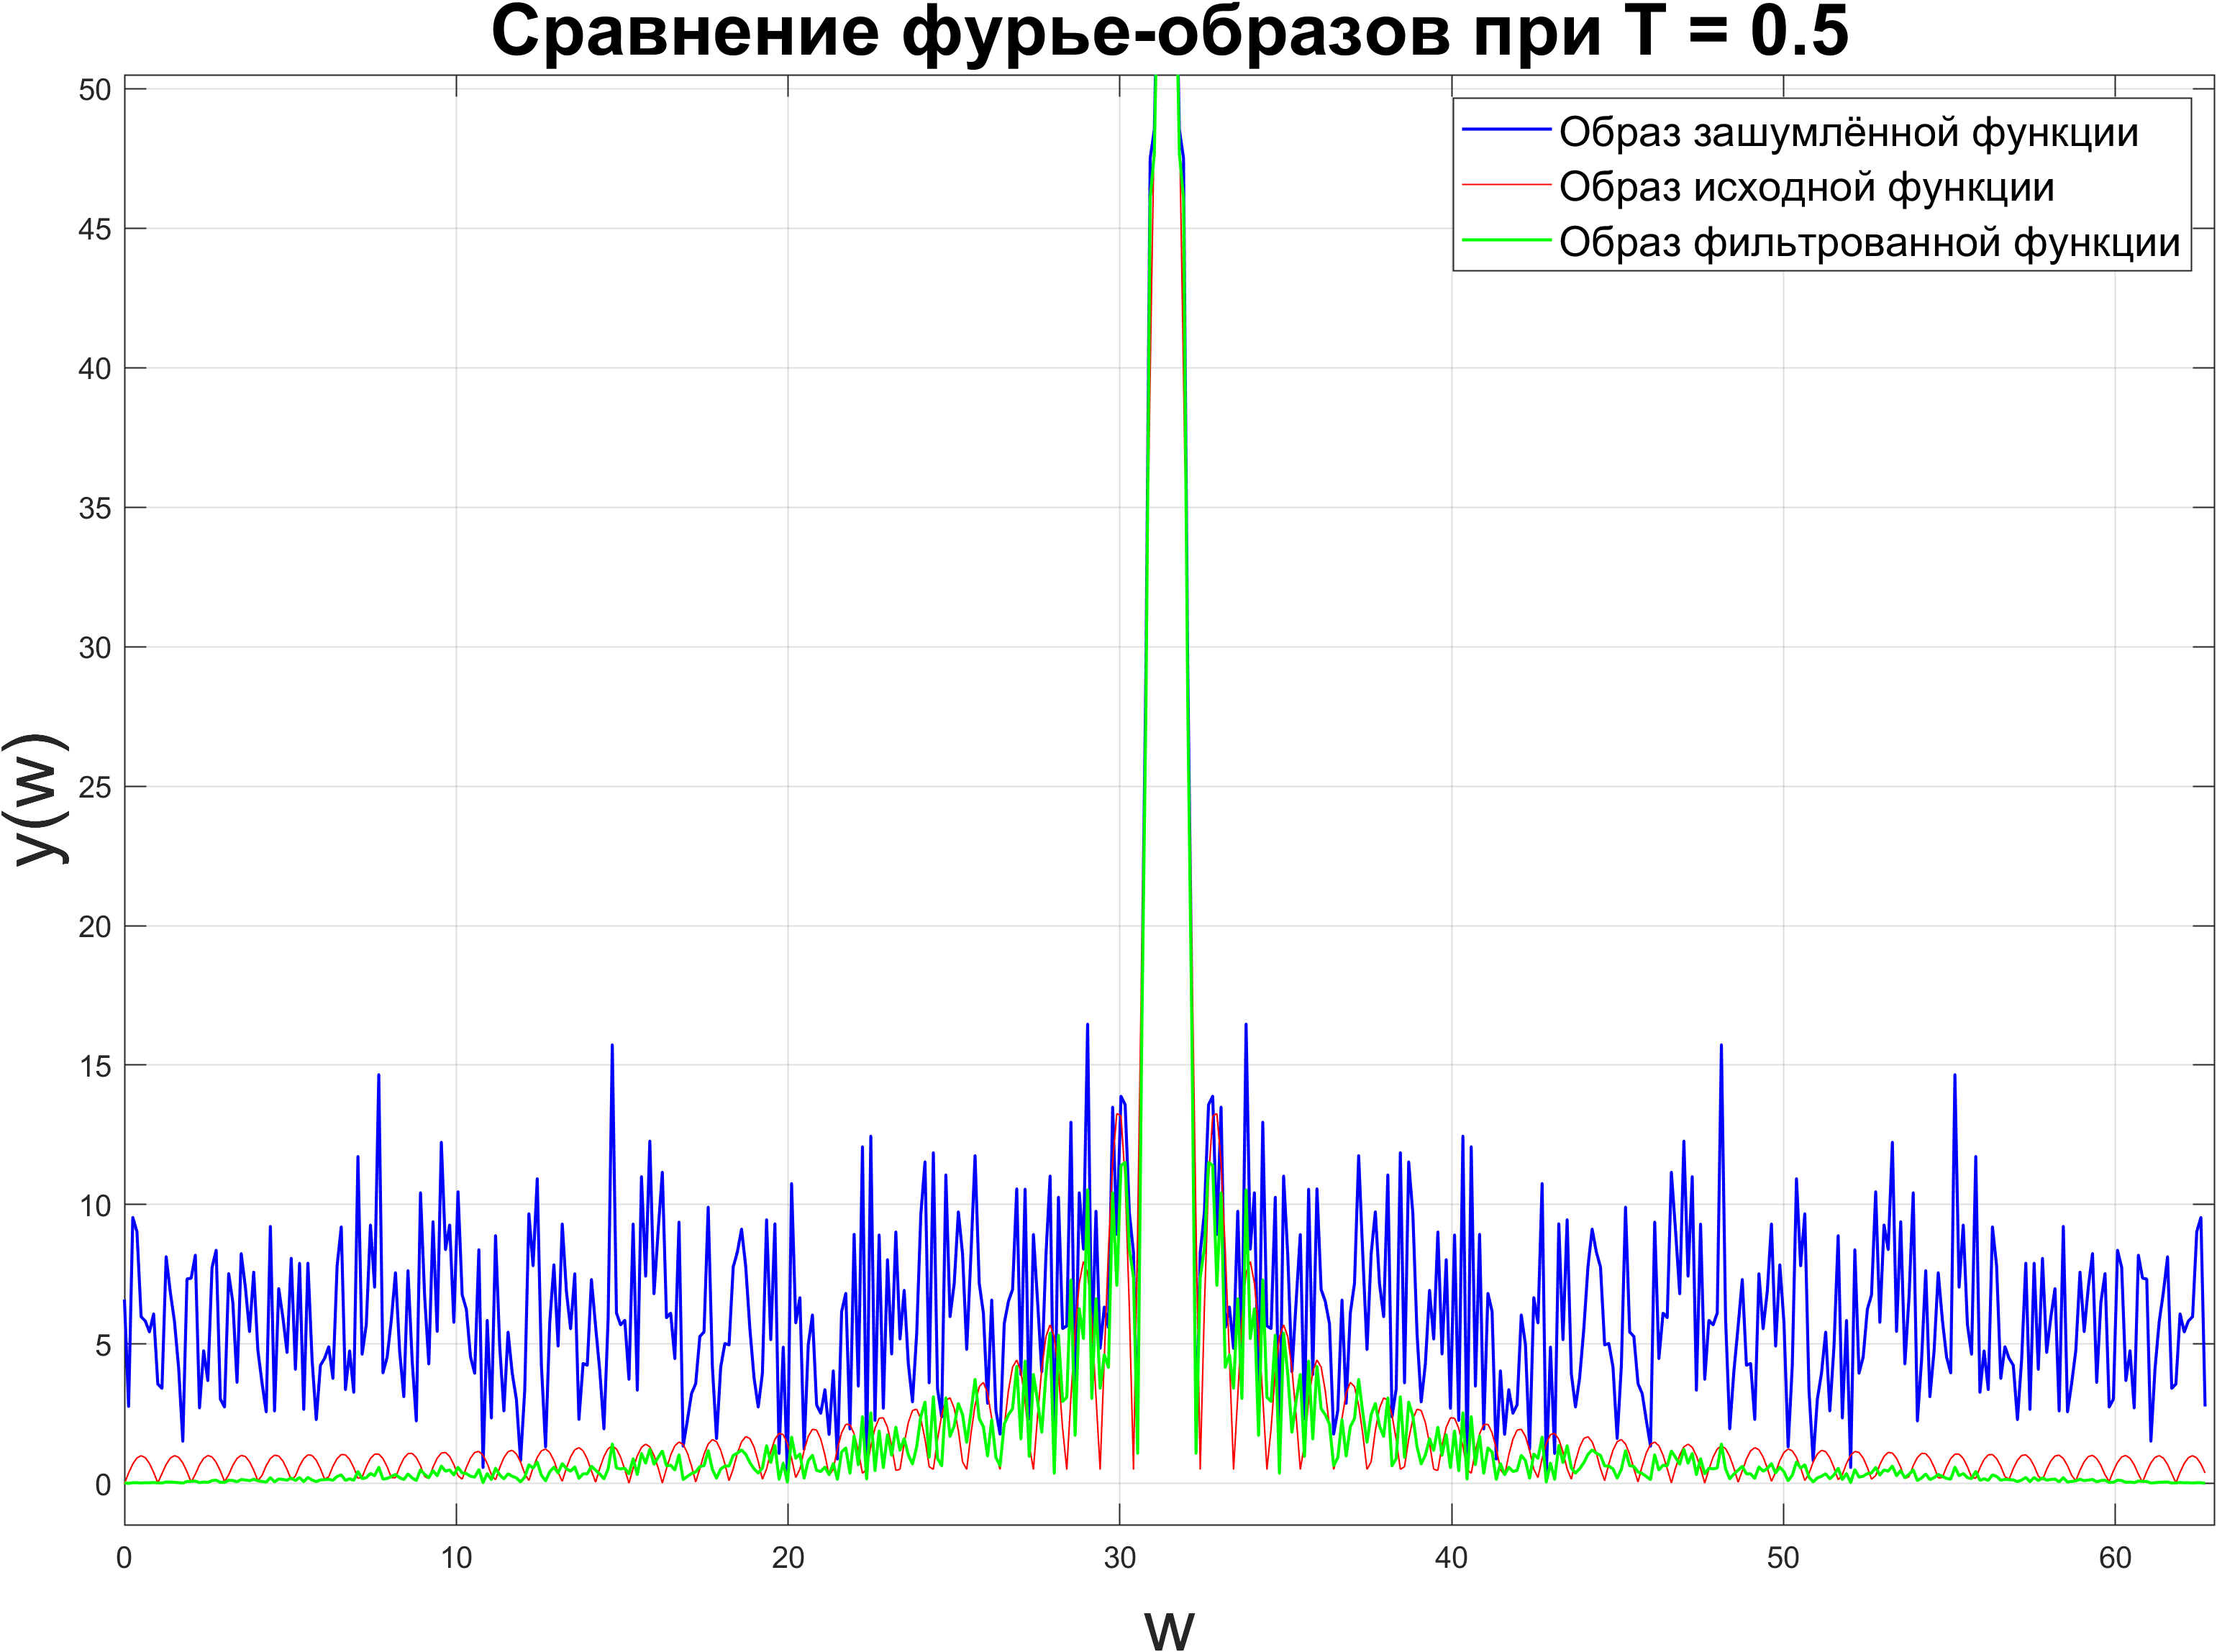
\includegraphics[width=0.80\textwidth, keepaspectratio]{images/fur_imgs_g_T_0.5.png}
    \caption{Фурье-образы при $T = 0.5$}
\end{figure}
\newpage

\begin{figure}[H]
    \centering
    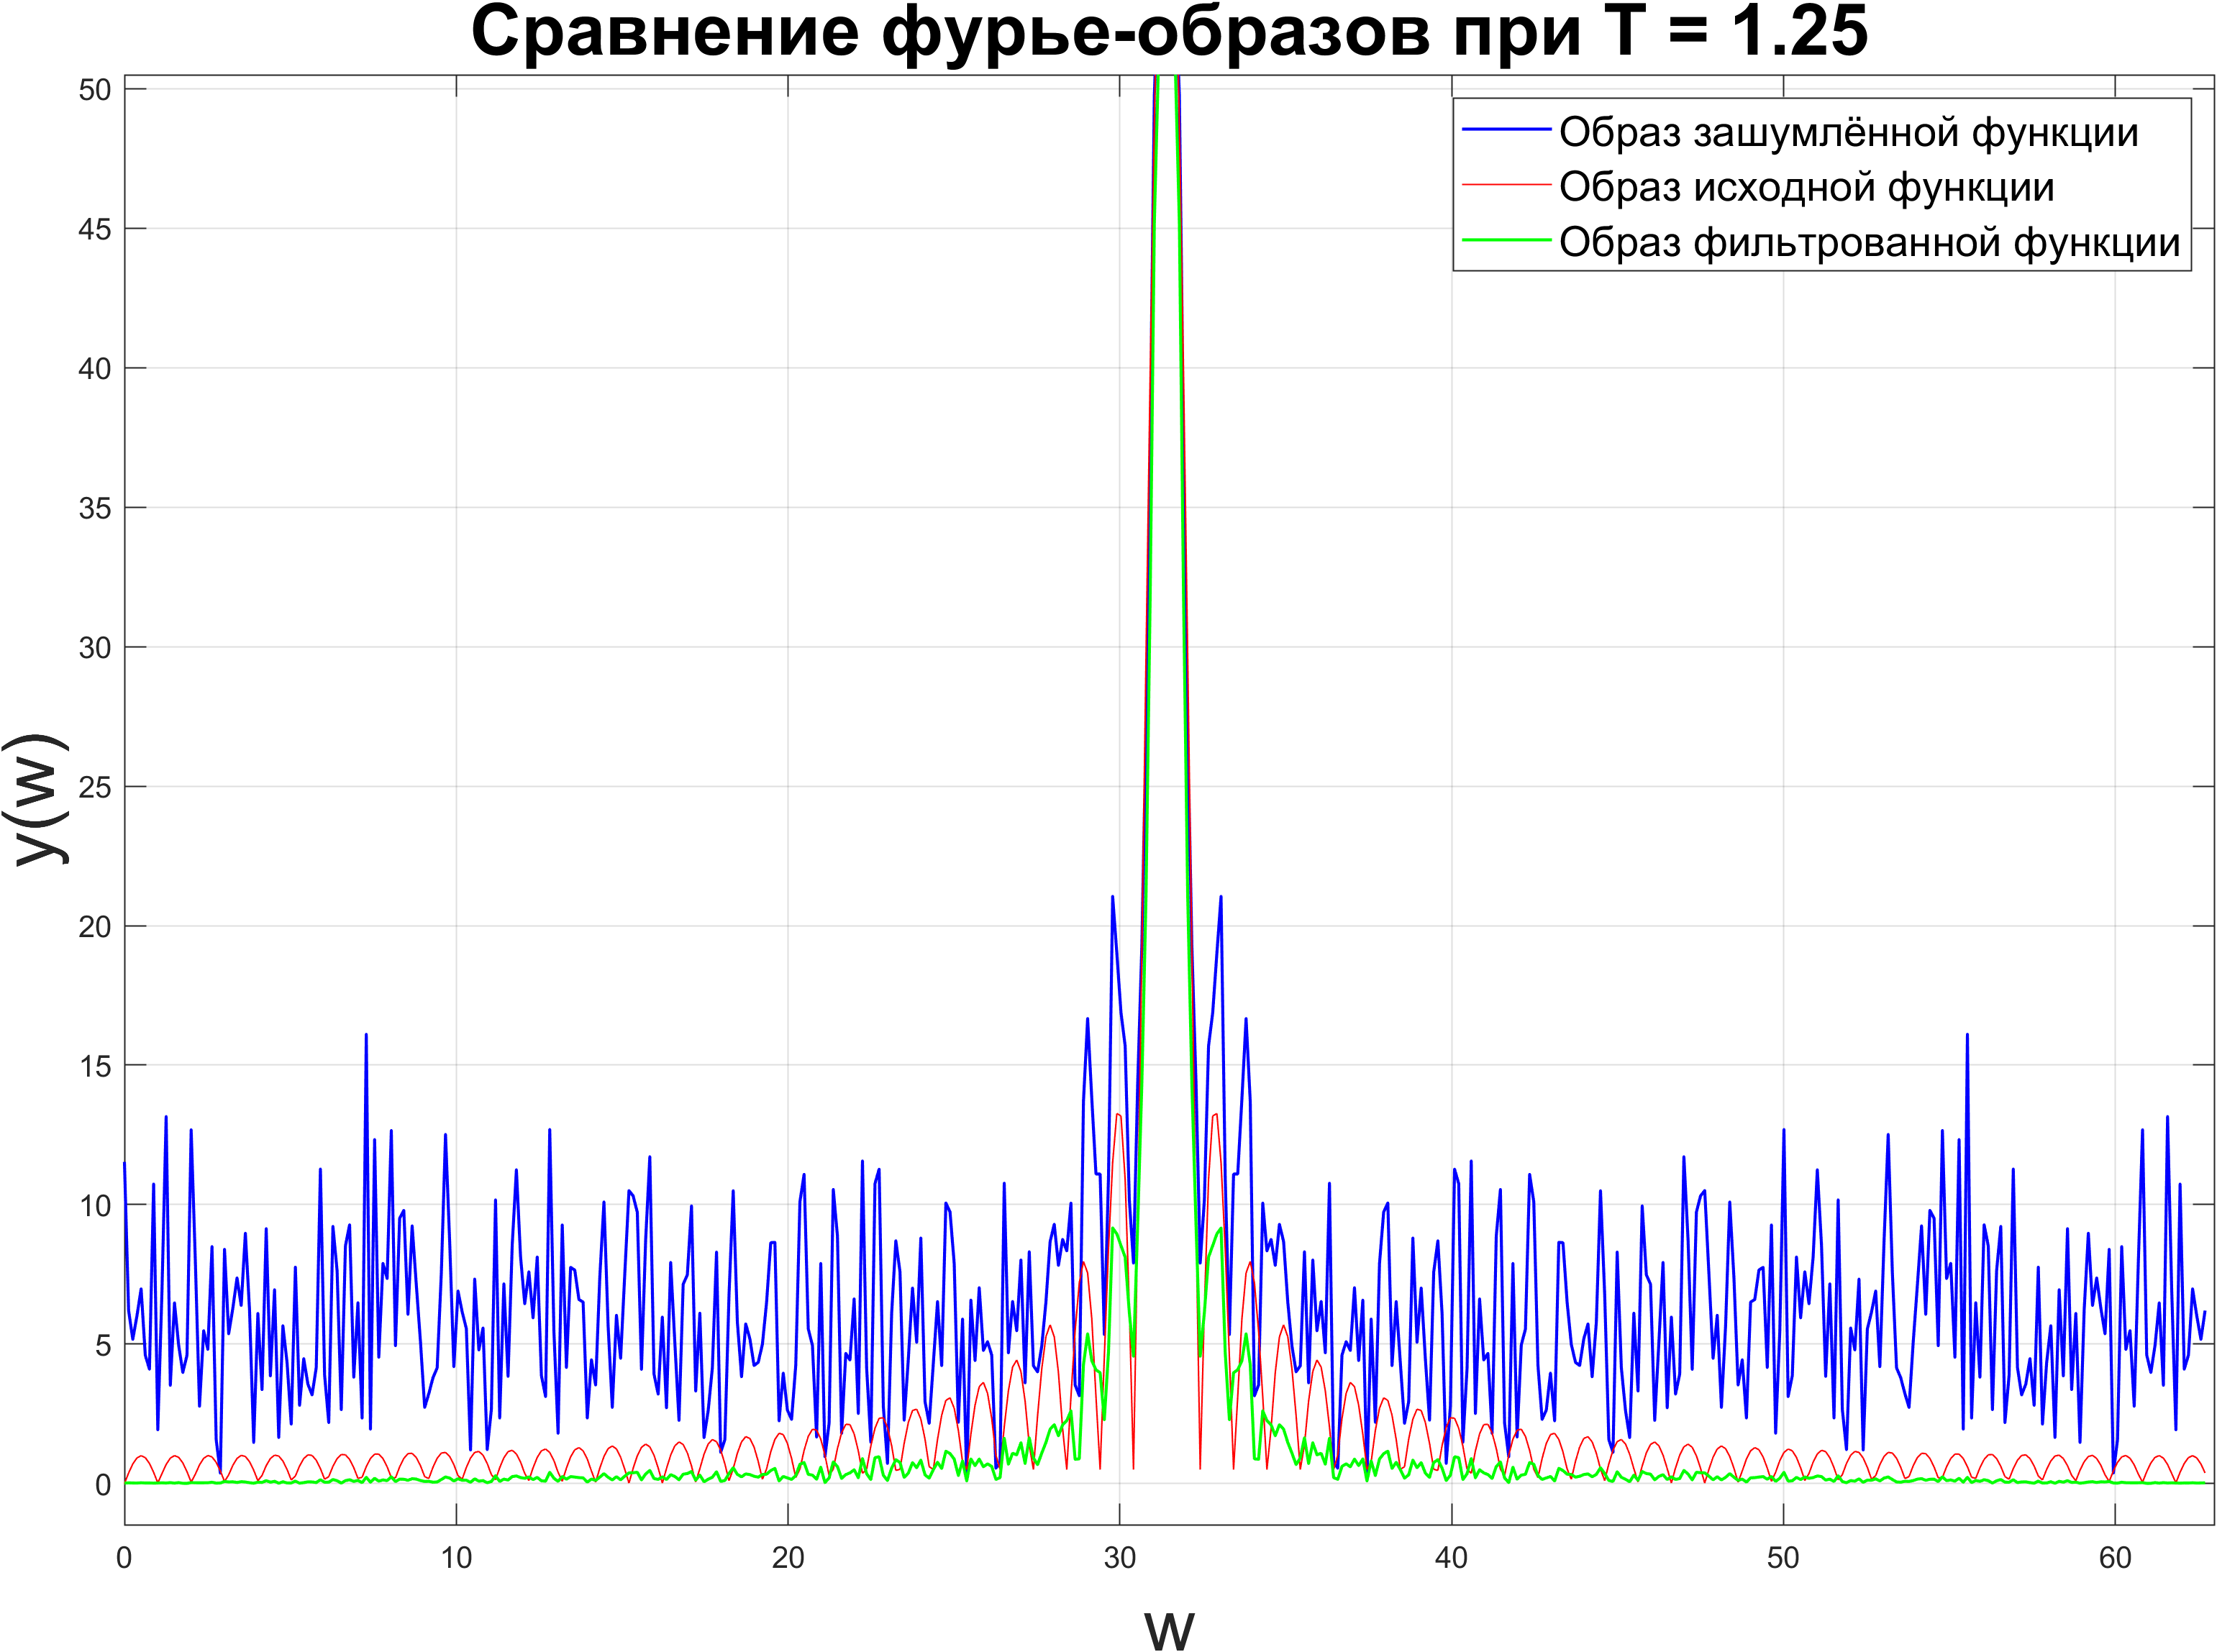
\includegraphics[width=0.90\textwidth, keepaspectratio]{images/fur_imgs_g_T_1.25.png}
    \caption{Фурье-образы при $T = 1.5$}
\end{figure}
\begin{figure}[H]
    \centering
    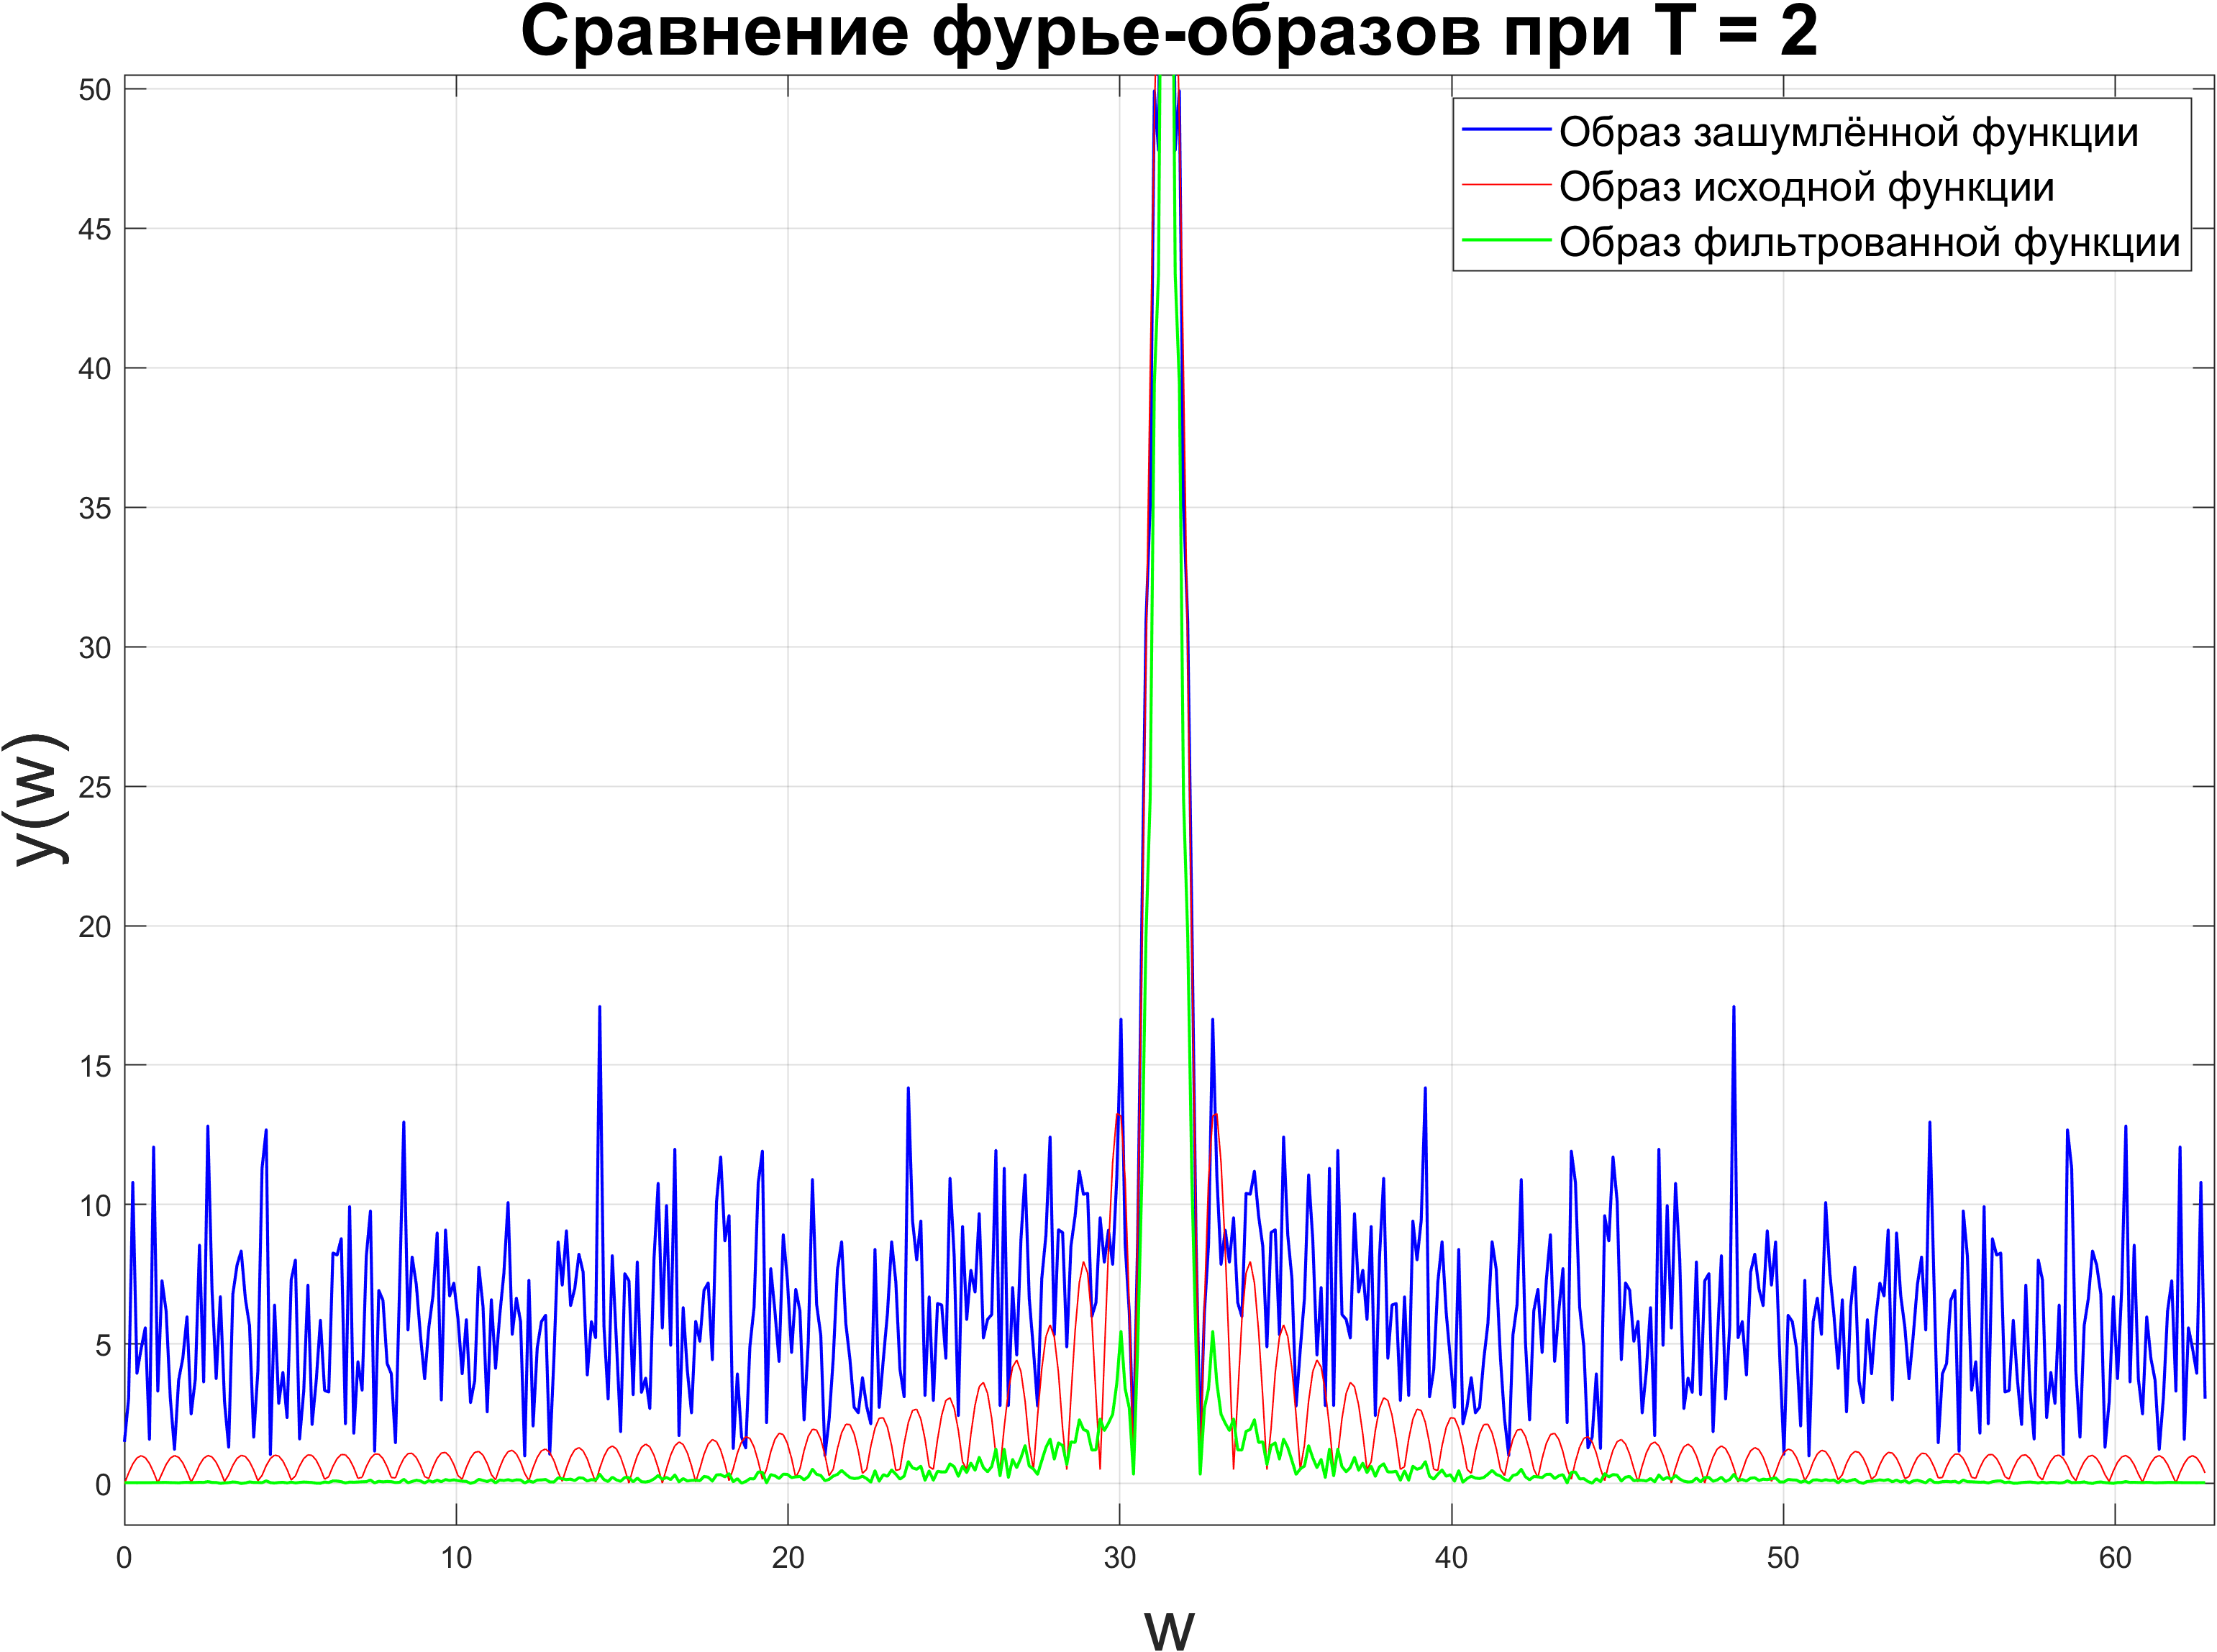
\includegraphics[width=0.90\textwidth, keepaspectratio]{images/fur_imgs_g_T_2.png}
    \caption{Фурье-образы при $T = 2.0$}
\end{figure}

\newpage
% ==========================================
% БЛОК 5: Фурье-образы (через передаточную функцию) при разных T
% ==========================================
\subsection{Фурье-образы $Y$, $y_{fil}$ (параметр $T$)}
Произведение передаточной функции на Фурье-образ выглядит достаточно близким к образу на положительной полуоси и близкой к нулю на отрицательной полуоси.

\begin{figure}[H]
    \centering
    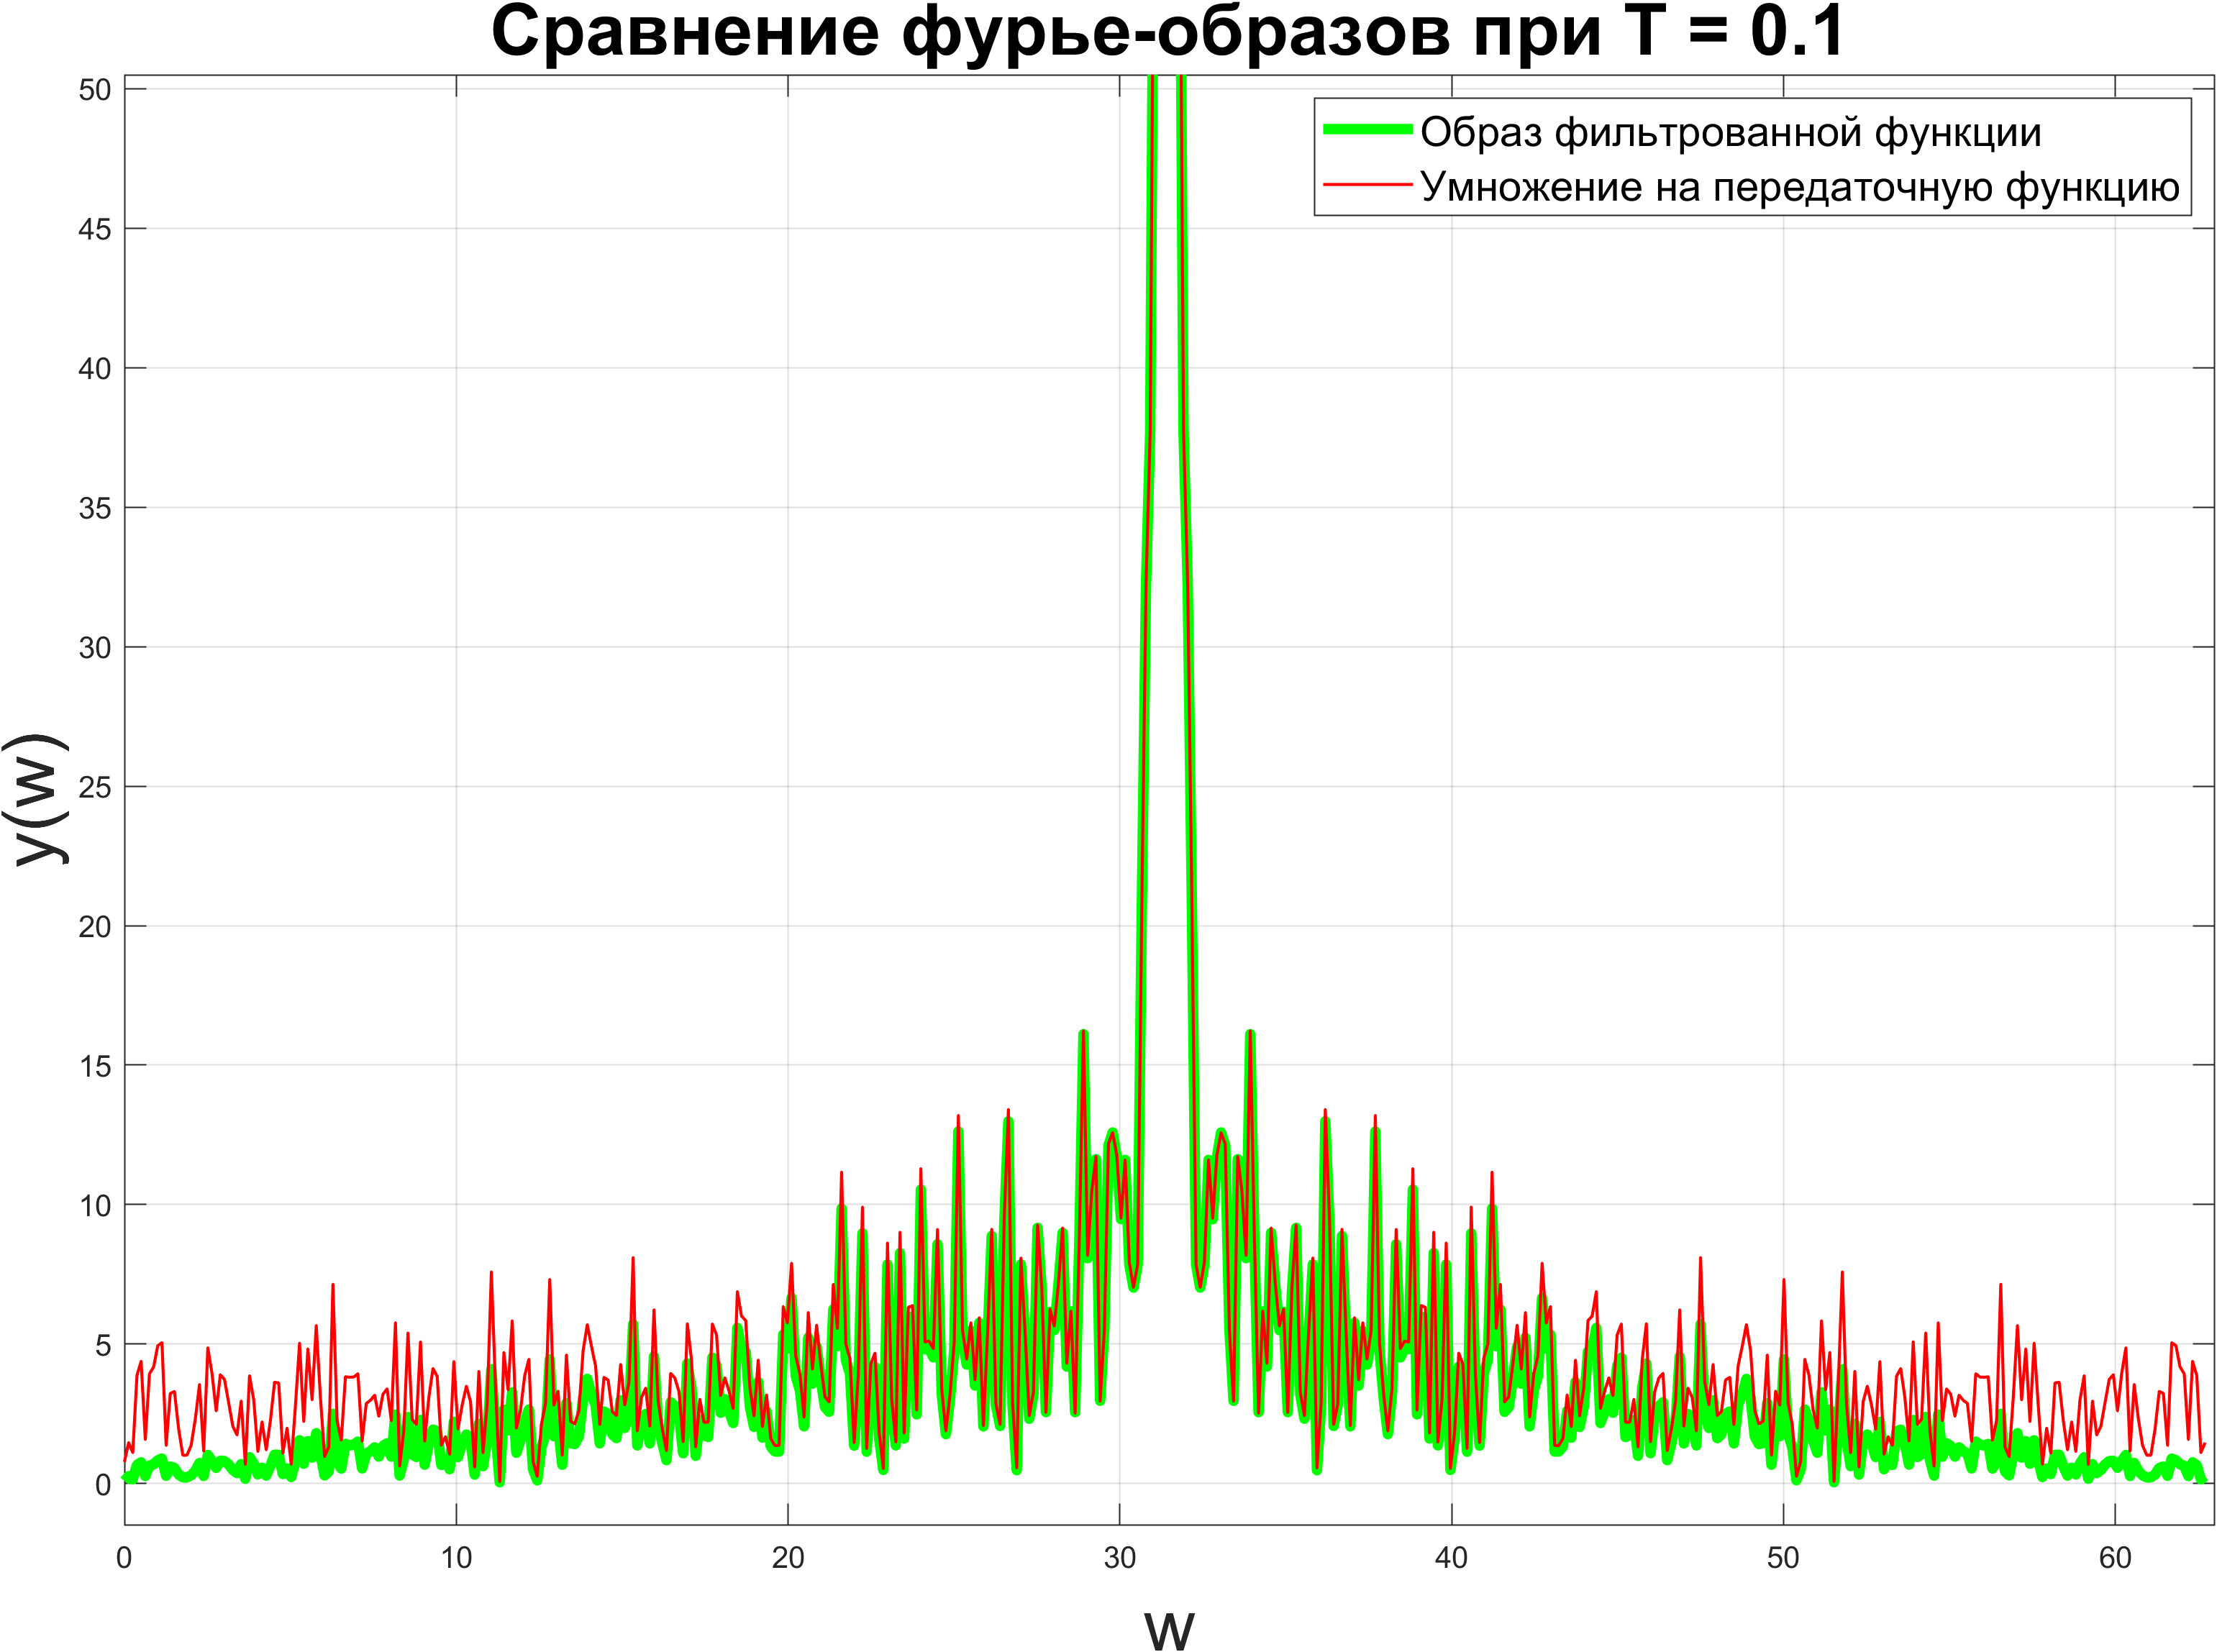
\includegraphics[width=0.80\textwidth, keepaspectratio]{images/fur_imgs_w_T_0.1.png}
    \caption{Фурье-образы через $H(\omega)$ при $T = 0.1$}
\end{figure}
\begin{figure}[H]
    \centering
    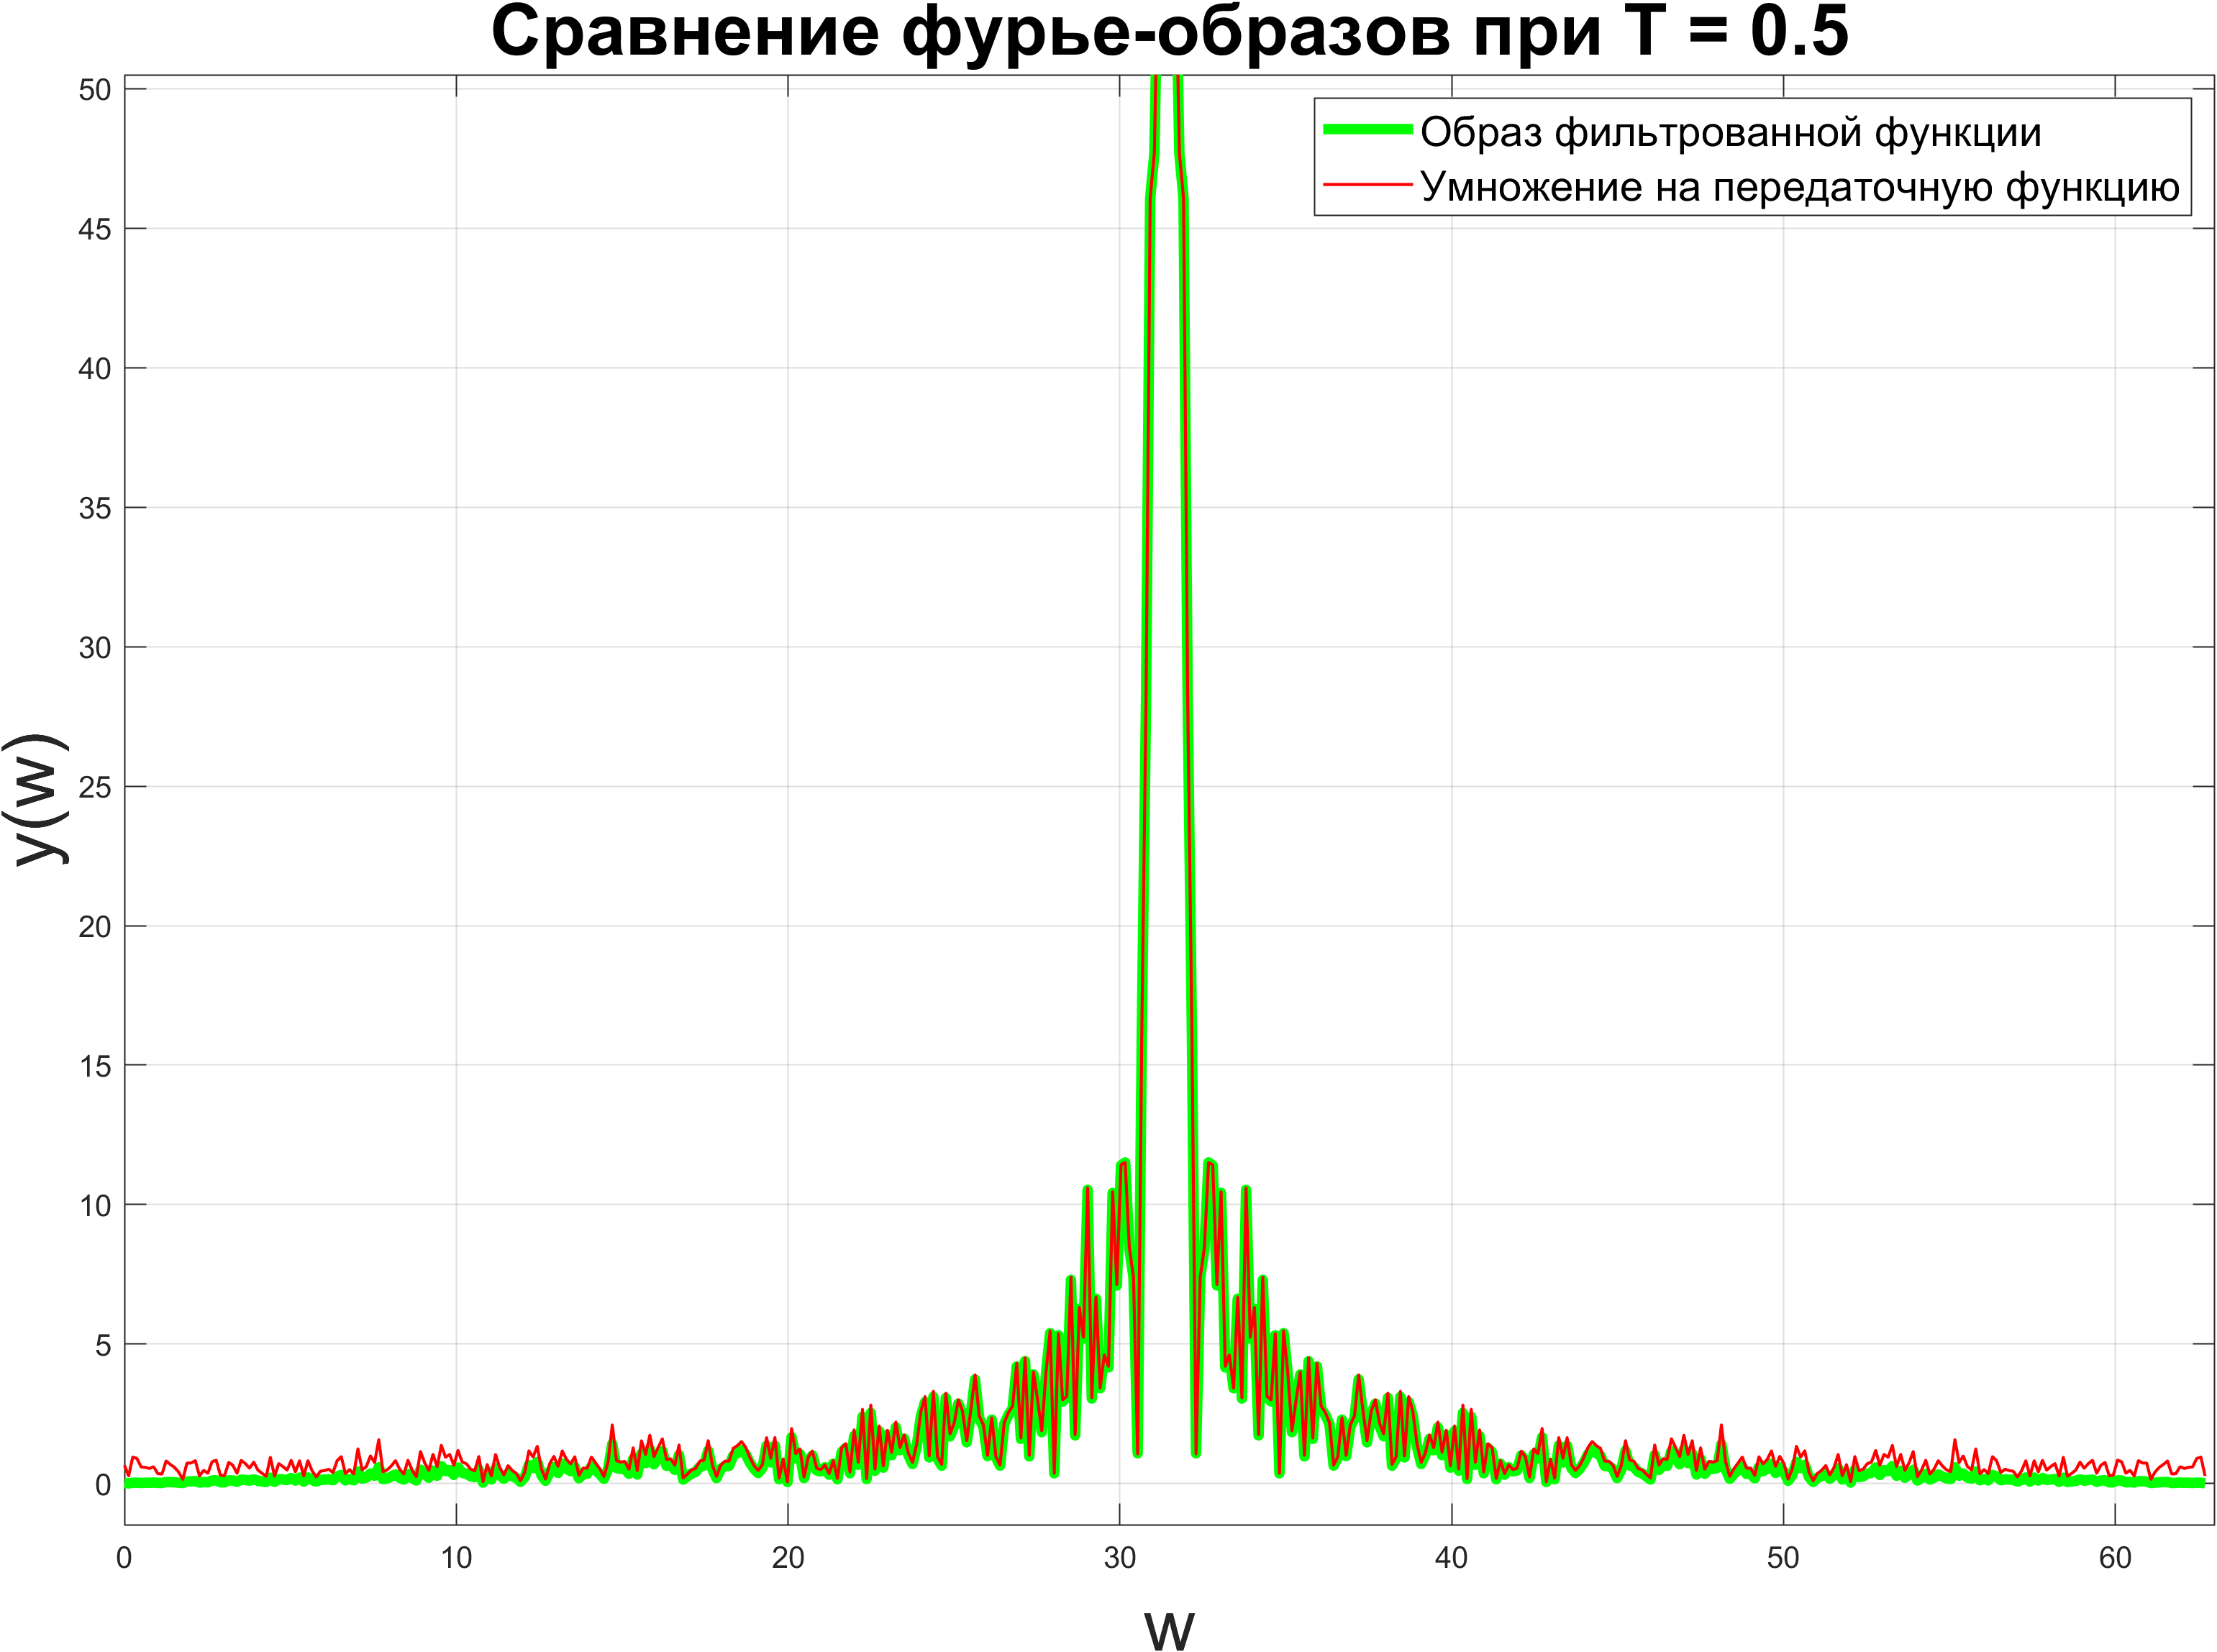
\includegraphics[width=0.80\textwidth, keepaspectratio]{images/fur_imgs_w_T_0.5.png}
    \caption{Фурье-образы через $H(\omega)$ при $T = 0.5$}
\end{figure}
\newpage

\begin{figure}[H]
    \centering
    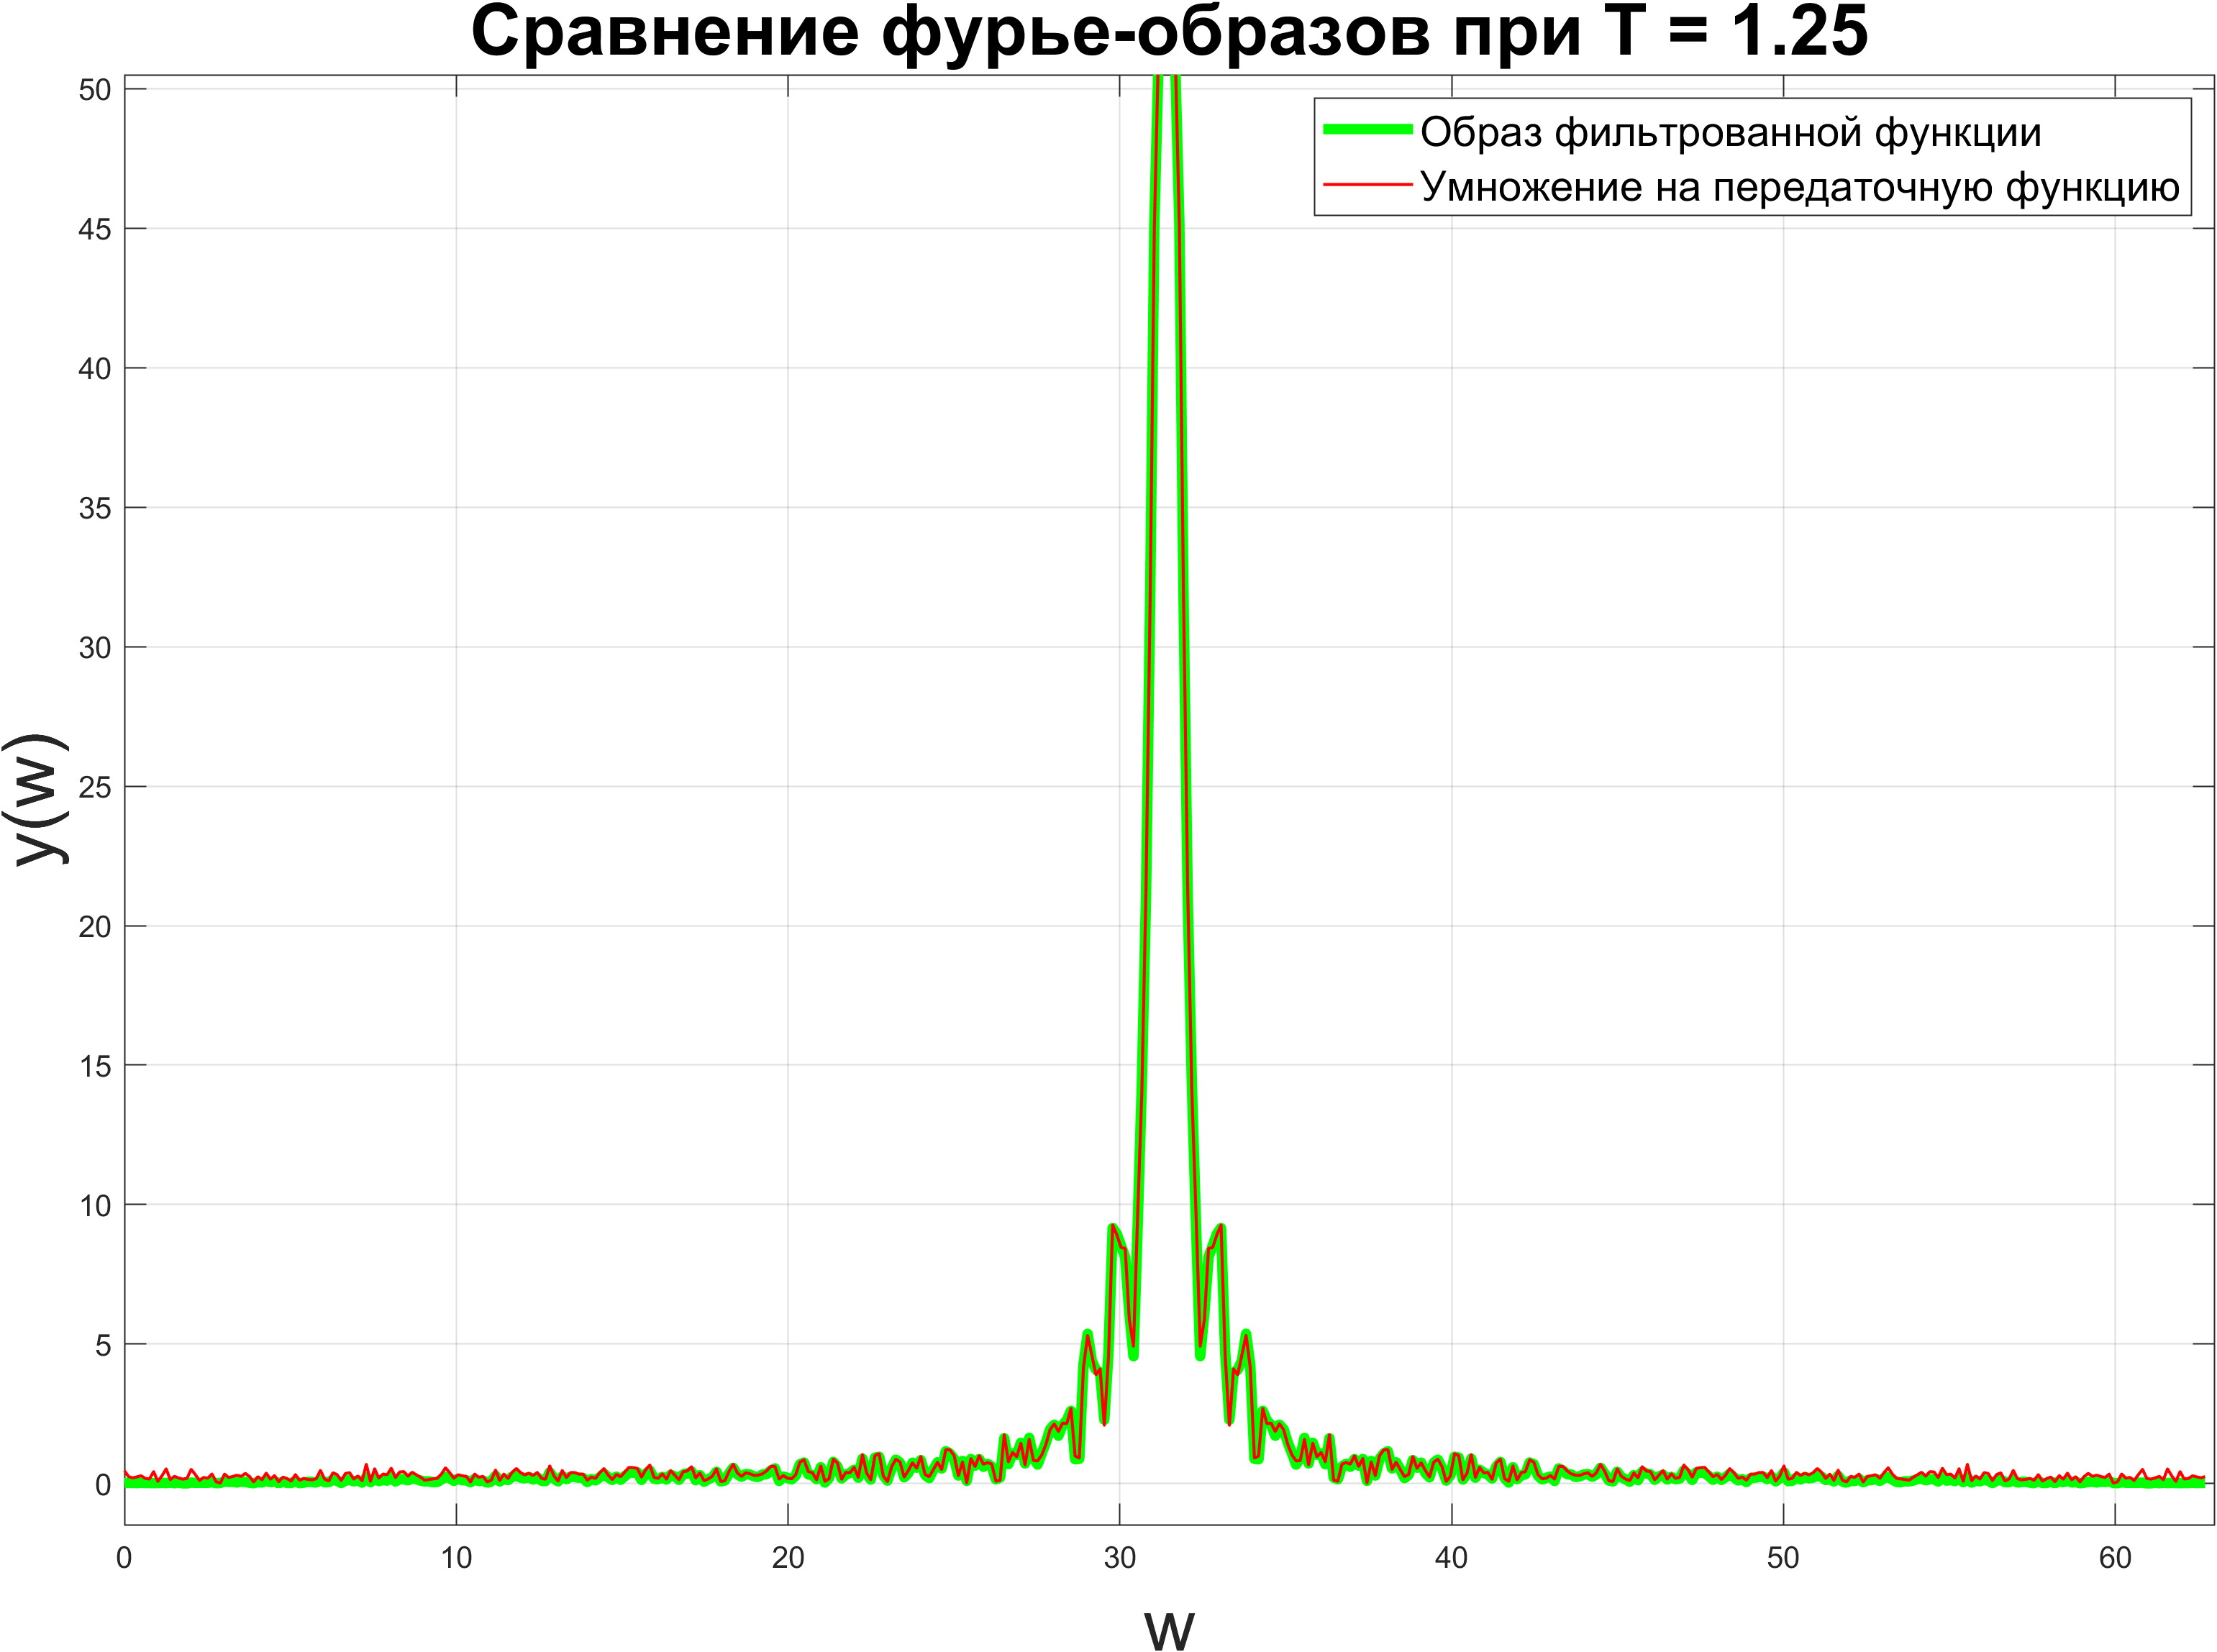
\includegraphics[width=0.90\textwidth, keepaspectratio]{images/fur_imgs_w_T_1.25.png}
    \caption{Фурье-образы через $H(\omega)$ при $T = 1.5$}
\end{figure}
\begin{figure}[H]
    \centering
    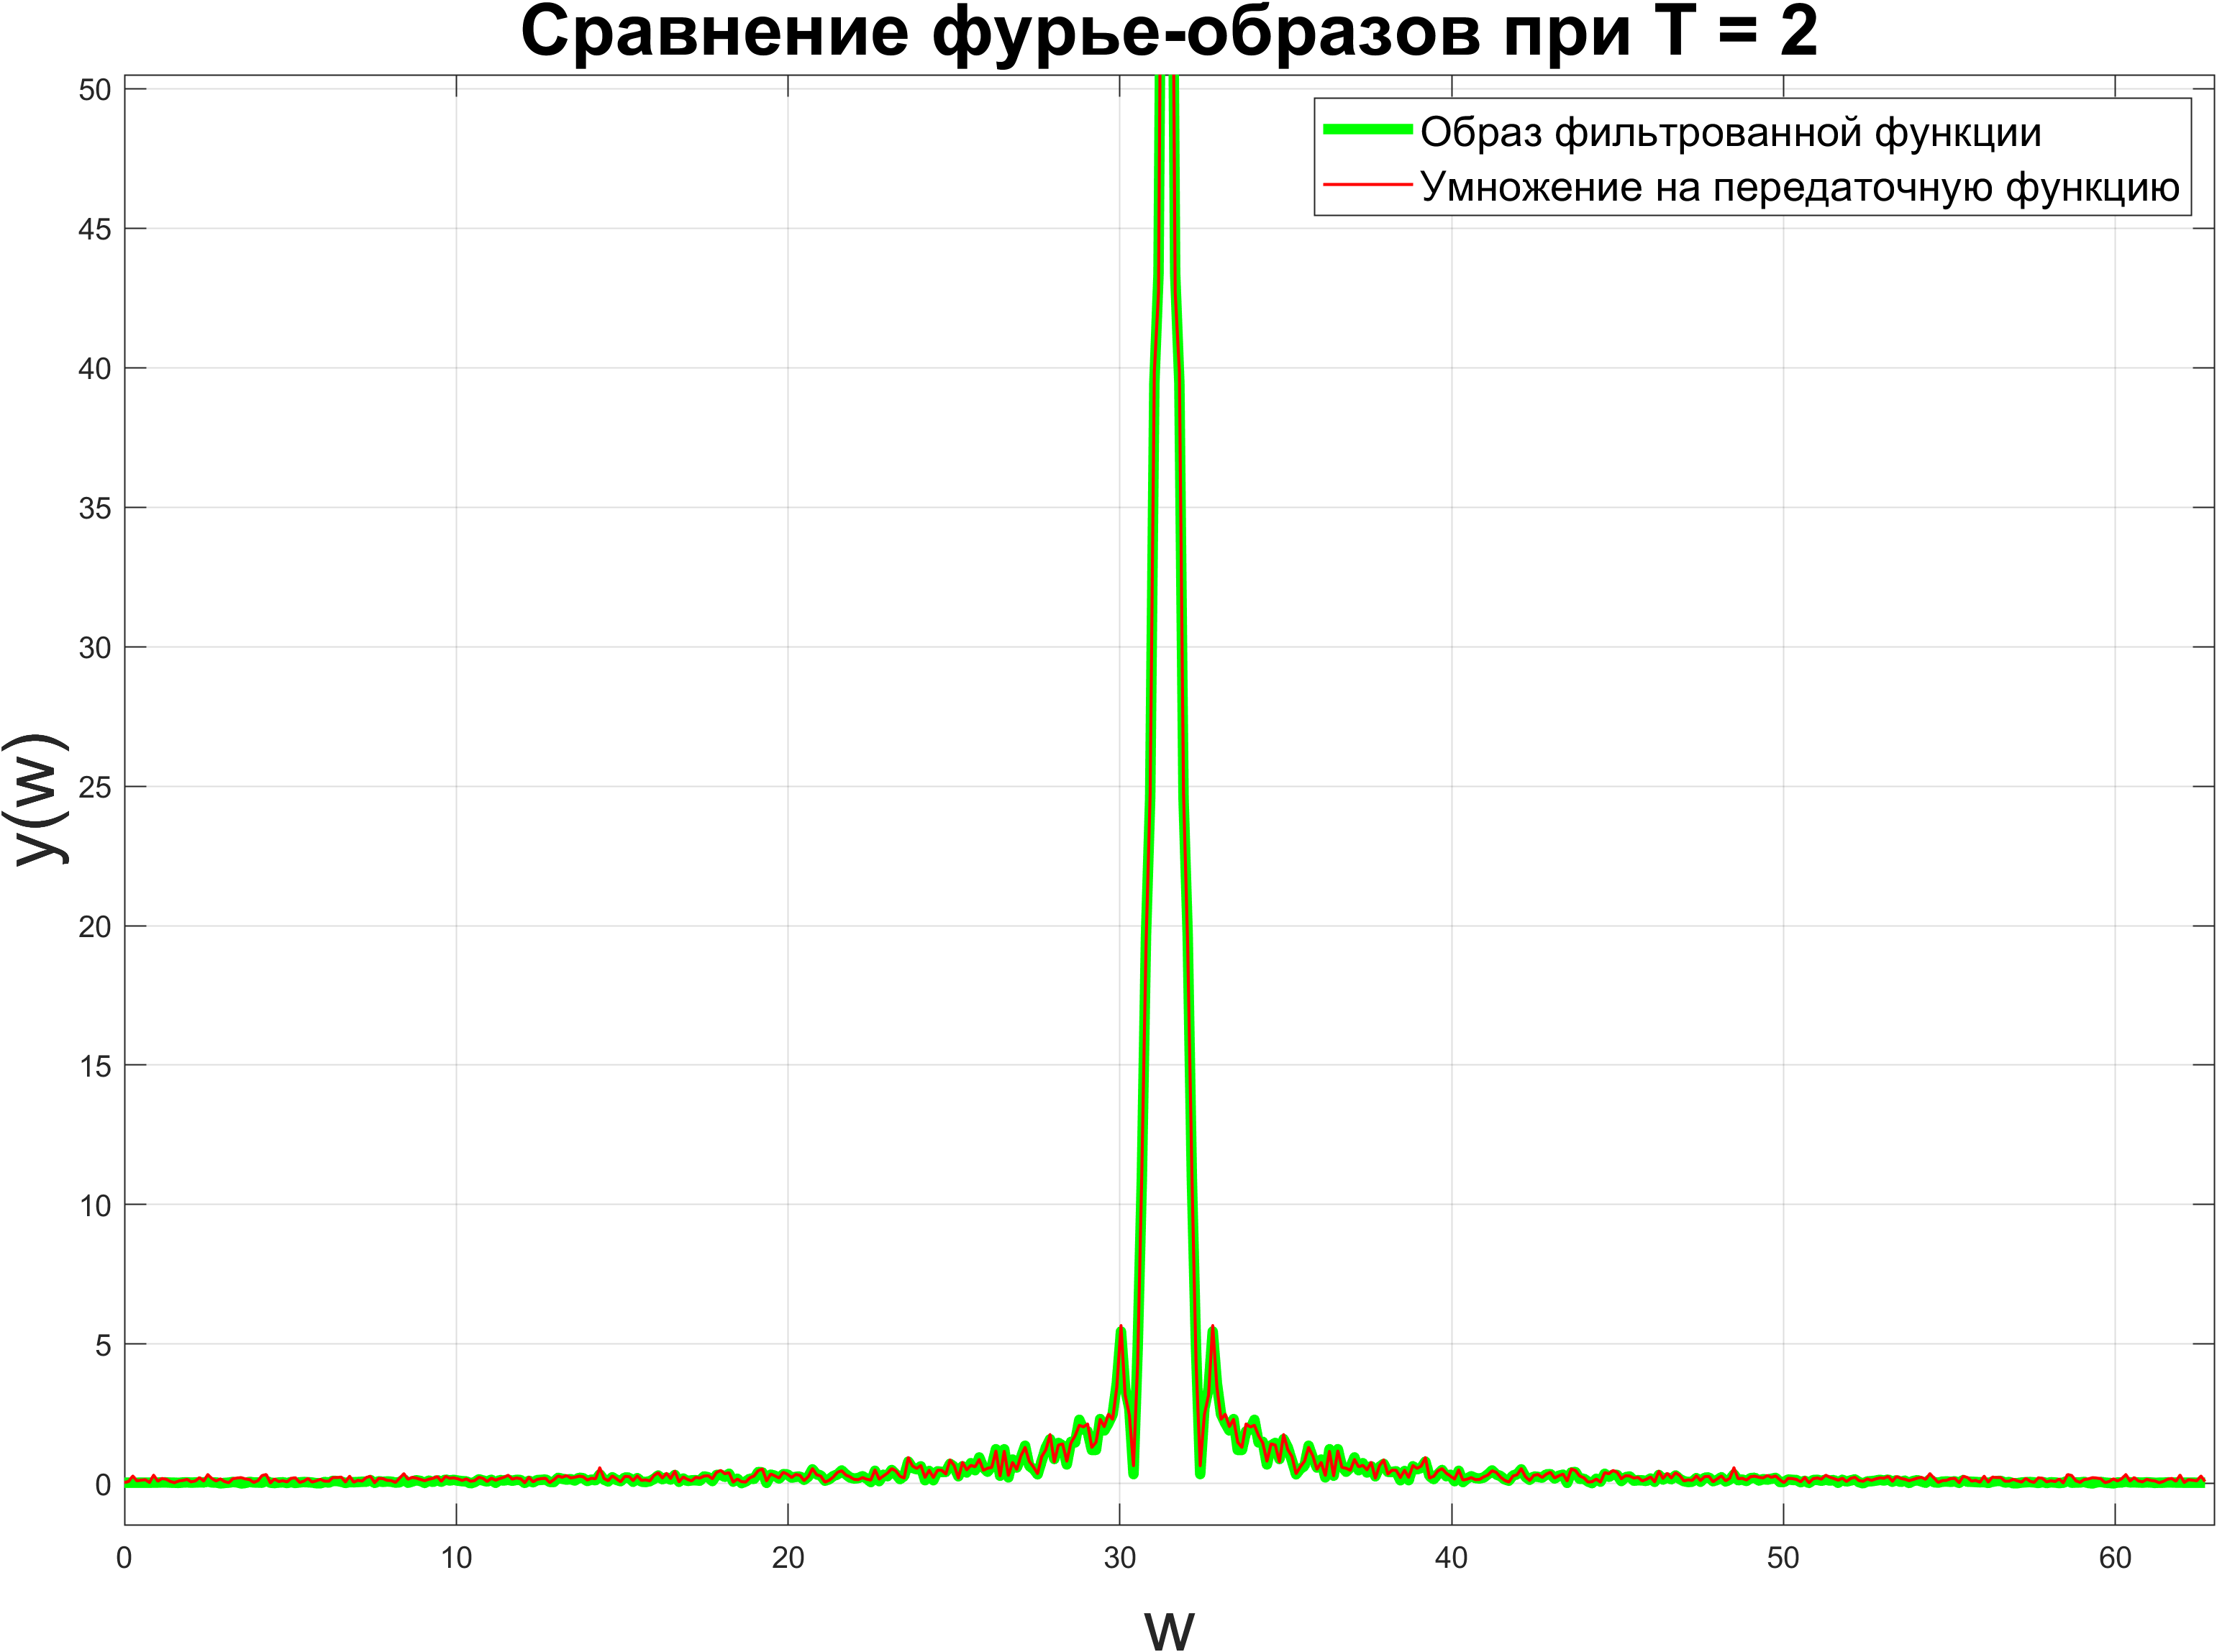
\includegraphics[width=0.90\textwidth, keepaspectratio]{images/fur_imgs_w_T_2.png}
    \caption{Фурье-образы через $H(\omega)$ при $T = 2.0$}
\end{figure}

% ==========================================
% БЛОК 7: Фильтрация сигнала при разных a
% ==========================================
\newpage
\subsection{Фильтрация сигнала (параметр $a$)}
При увеличении параметра \(a\) происходит почти такое же изменение как и при увеличении \(T\). В дальнейших пунктах графики ведут себя аналогично случаю с увеличением \(T\)

\begin{figure}[H]
    \centering
    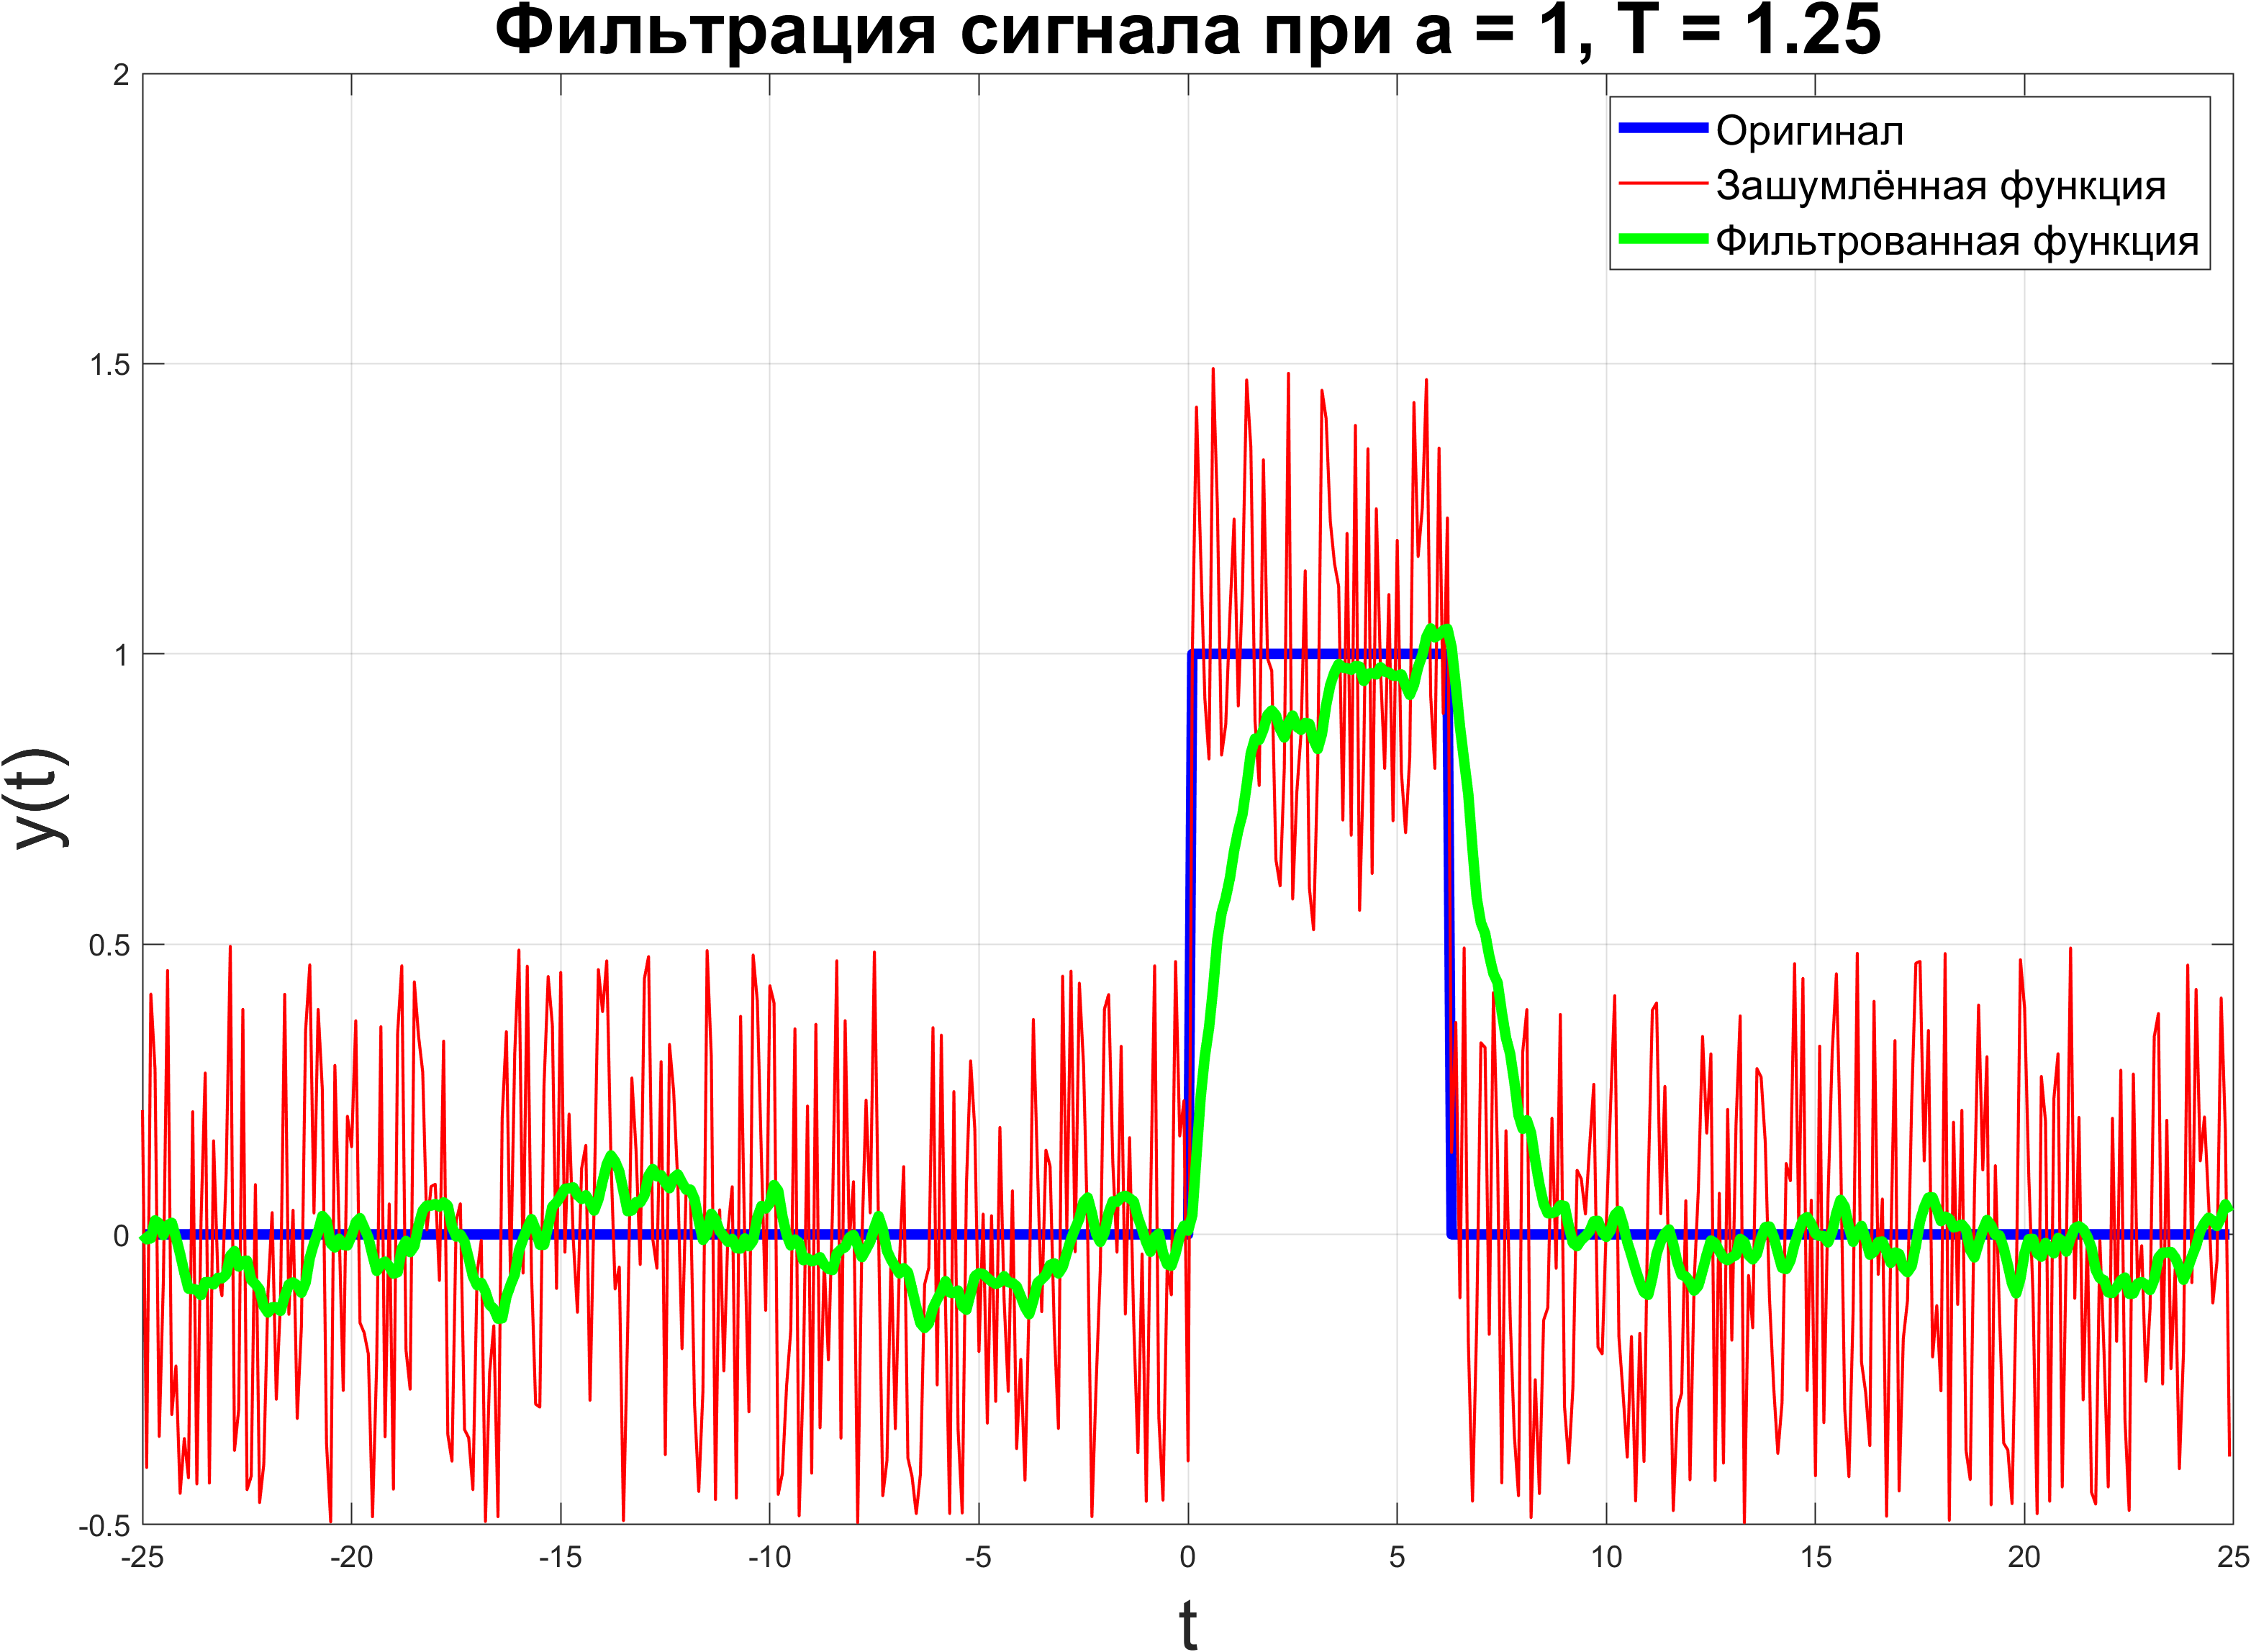
\includegraphics[width=0.80\textwidth, keepaspectratio]{images/filter_a_1.png}
    \caption{Фильтрация при $a = 1.0$}
\end{figure}
\begin{figure}[H]
    \centering
    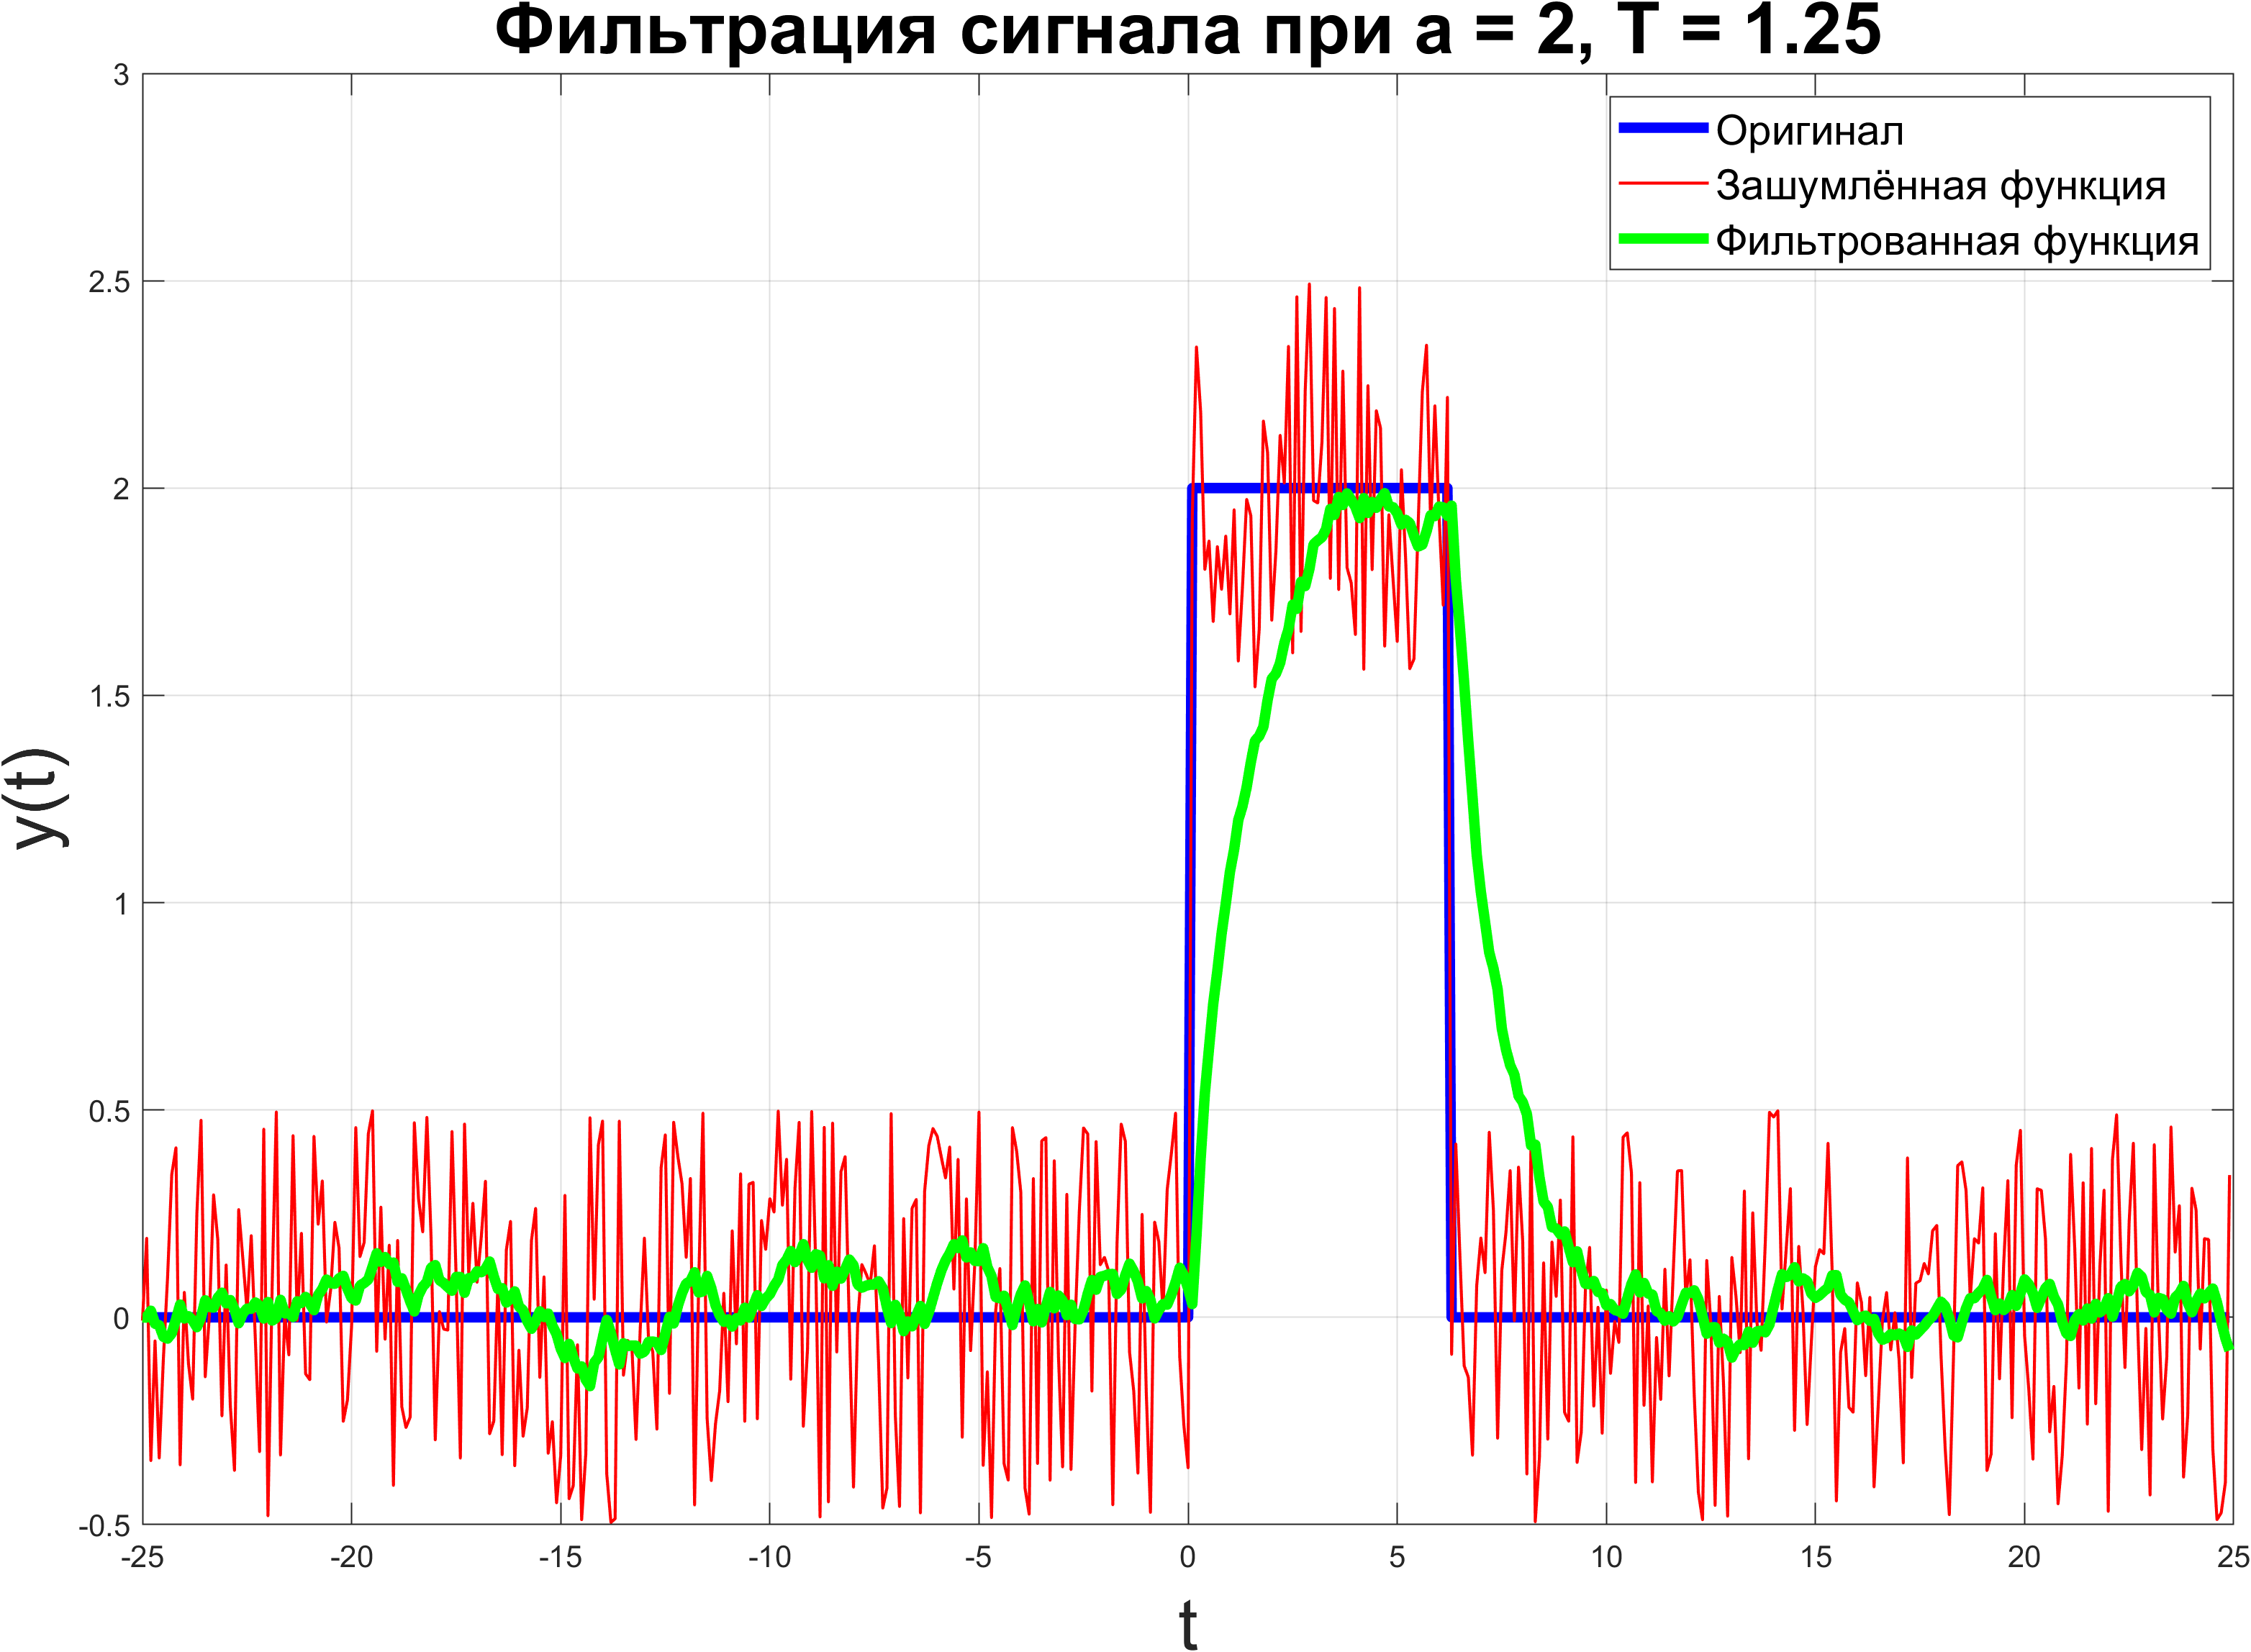
\includegraphics[width=0.80\textwidth, keepaspectratio]{images/filter_a_2.png}
    \caption{Фильтрация при $a = 2.0$}
\end{figure}
\newpage

\begin{figure}[H]
    \centering
    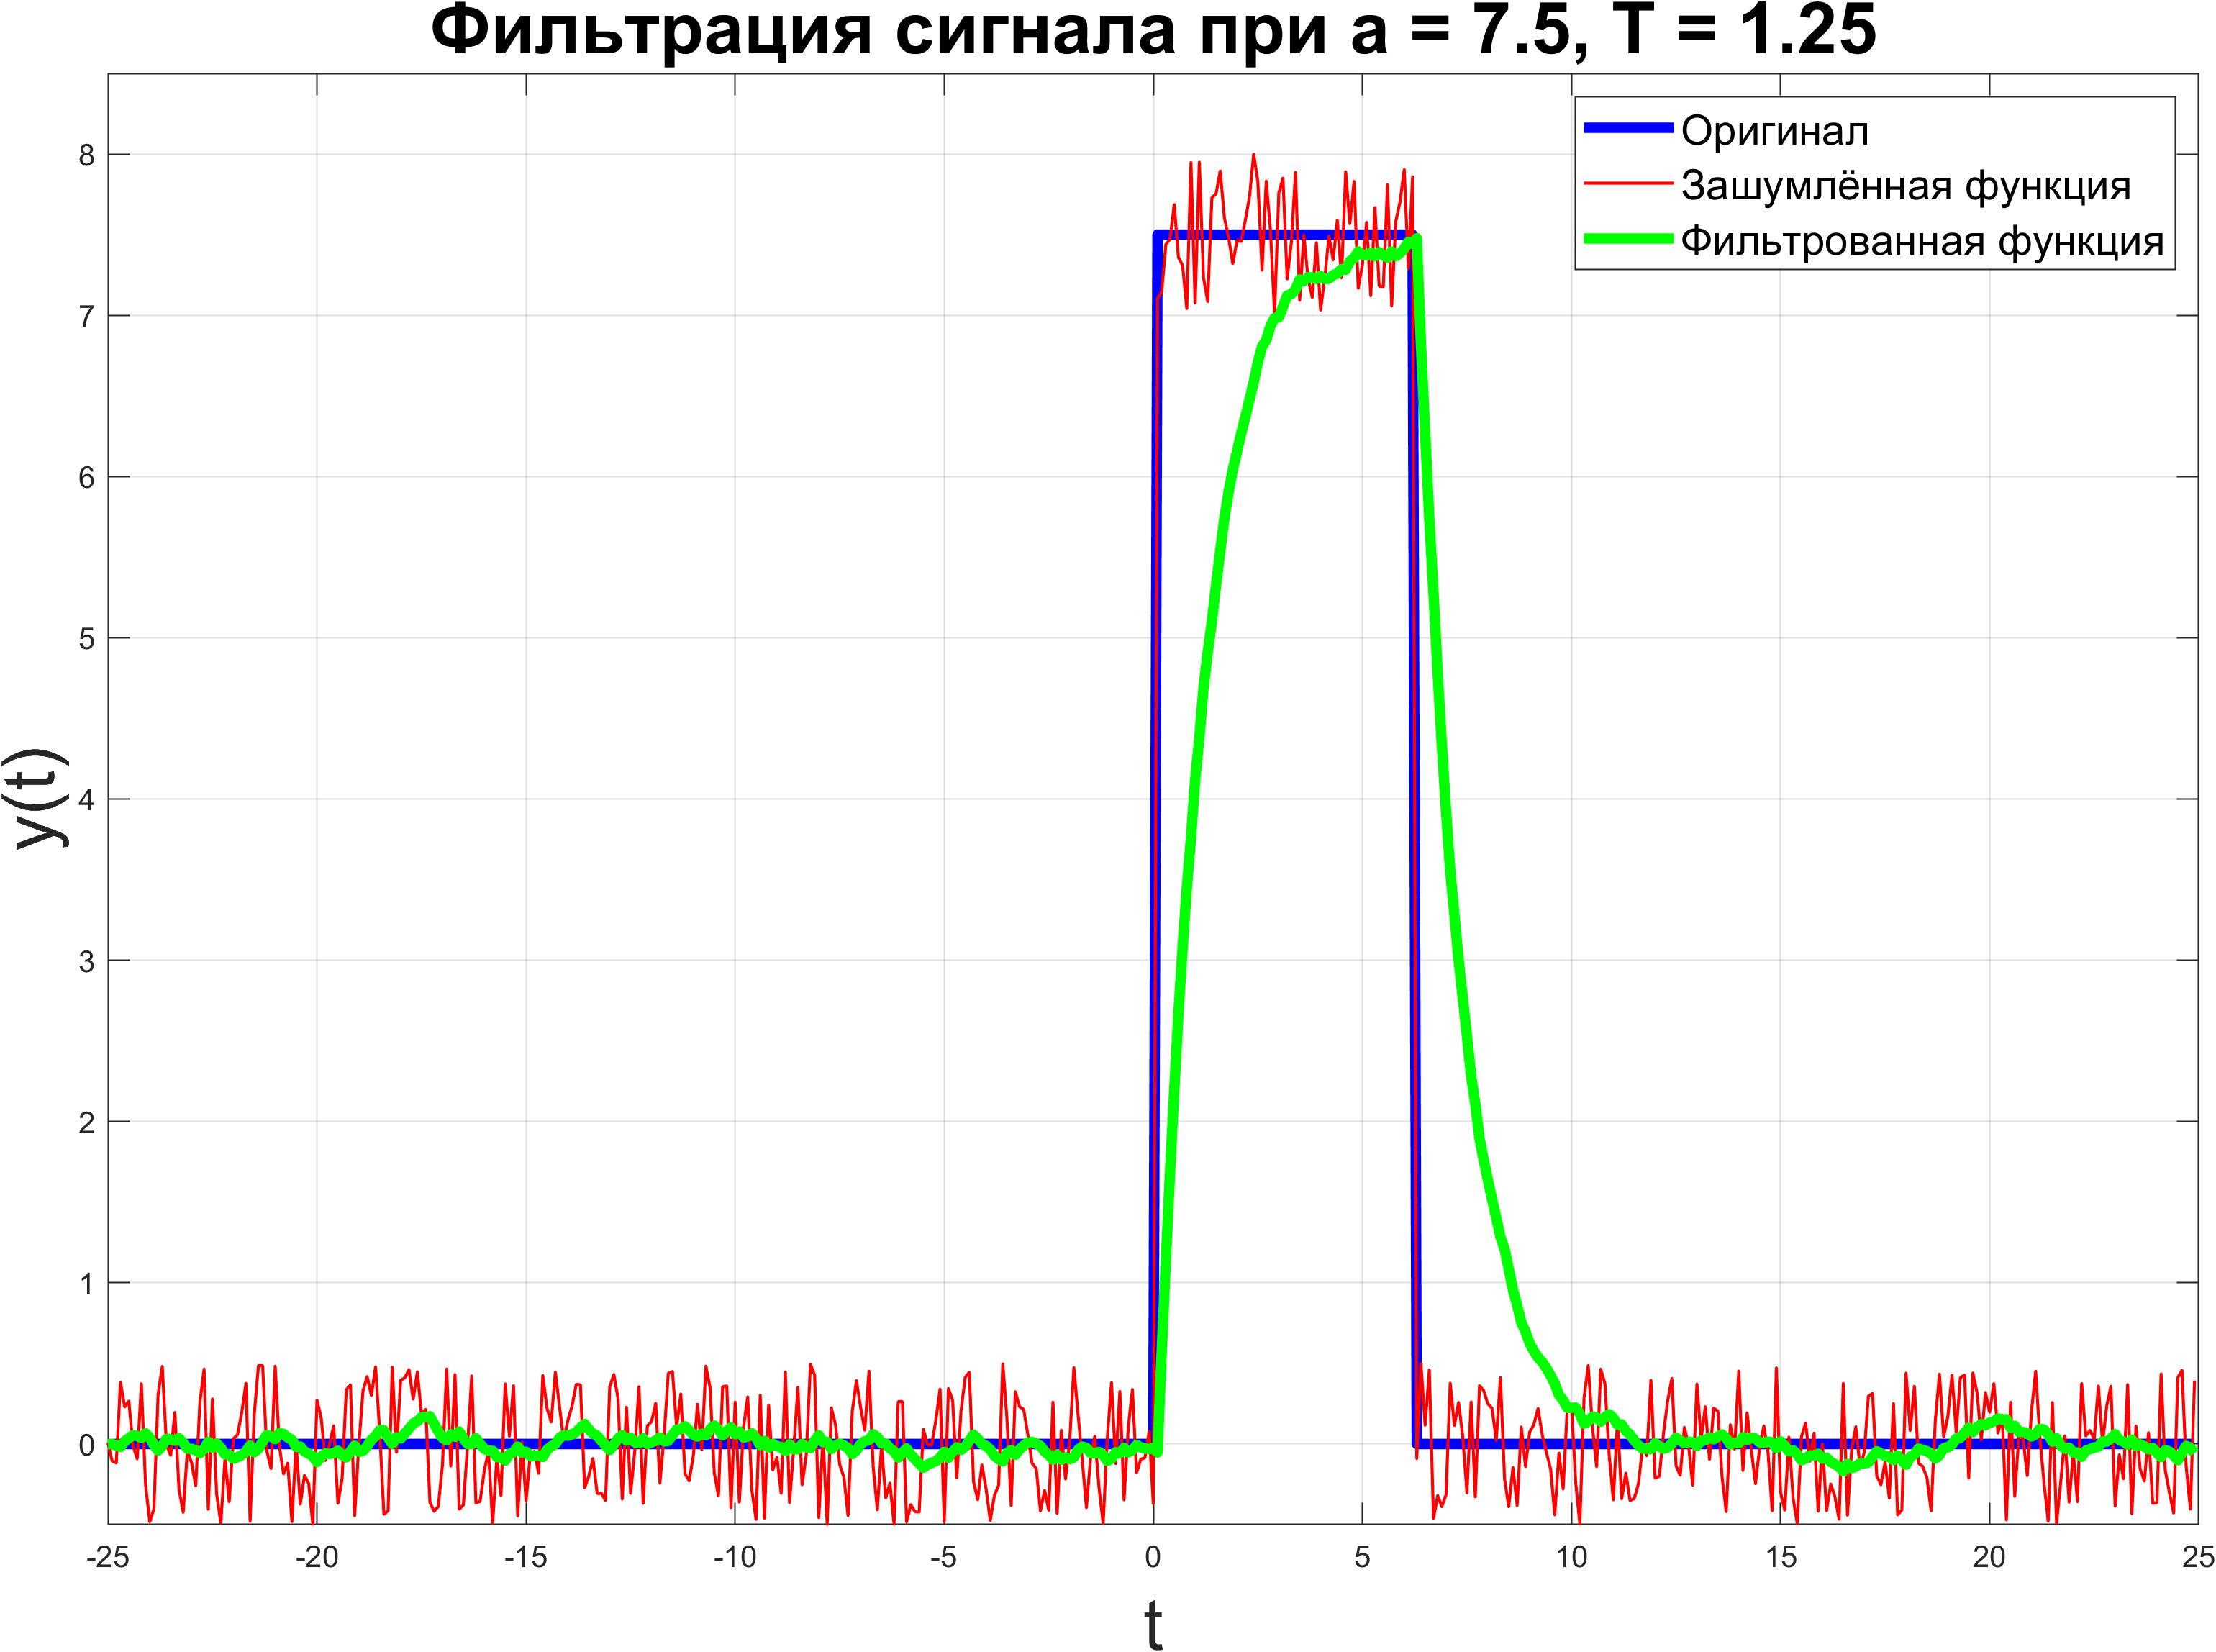
\includegraphics[width=0.92\textwidth, keepaspectratio]{images/filter_a_7.5.png}
    \caption{Фильтрация при $a = 7.5$}
\end{figure}
\begin{figure}[H]
    \centering
    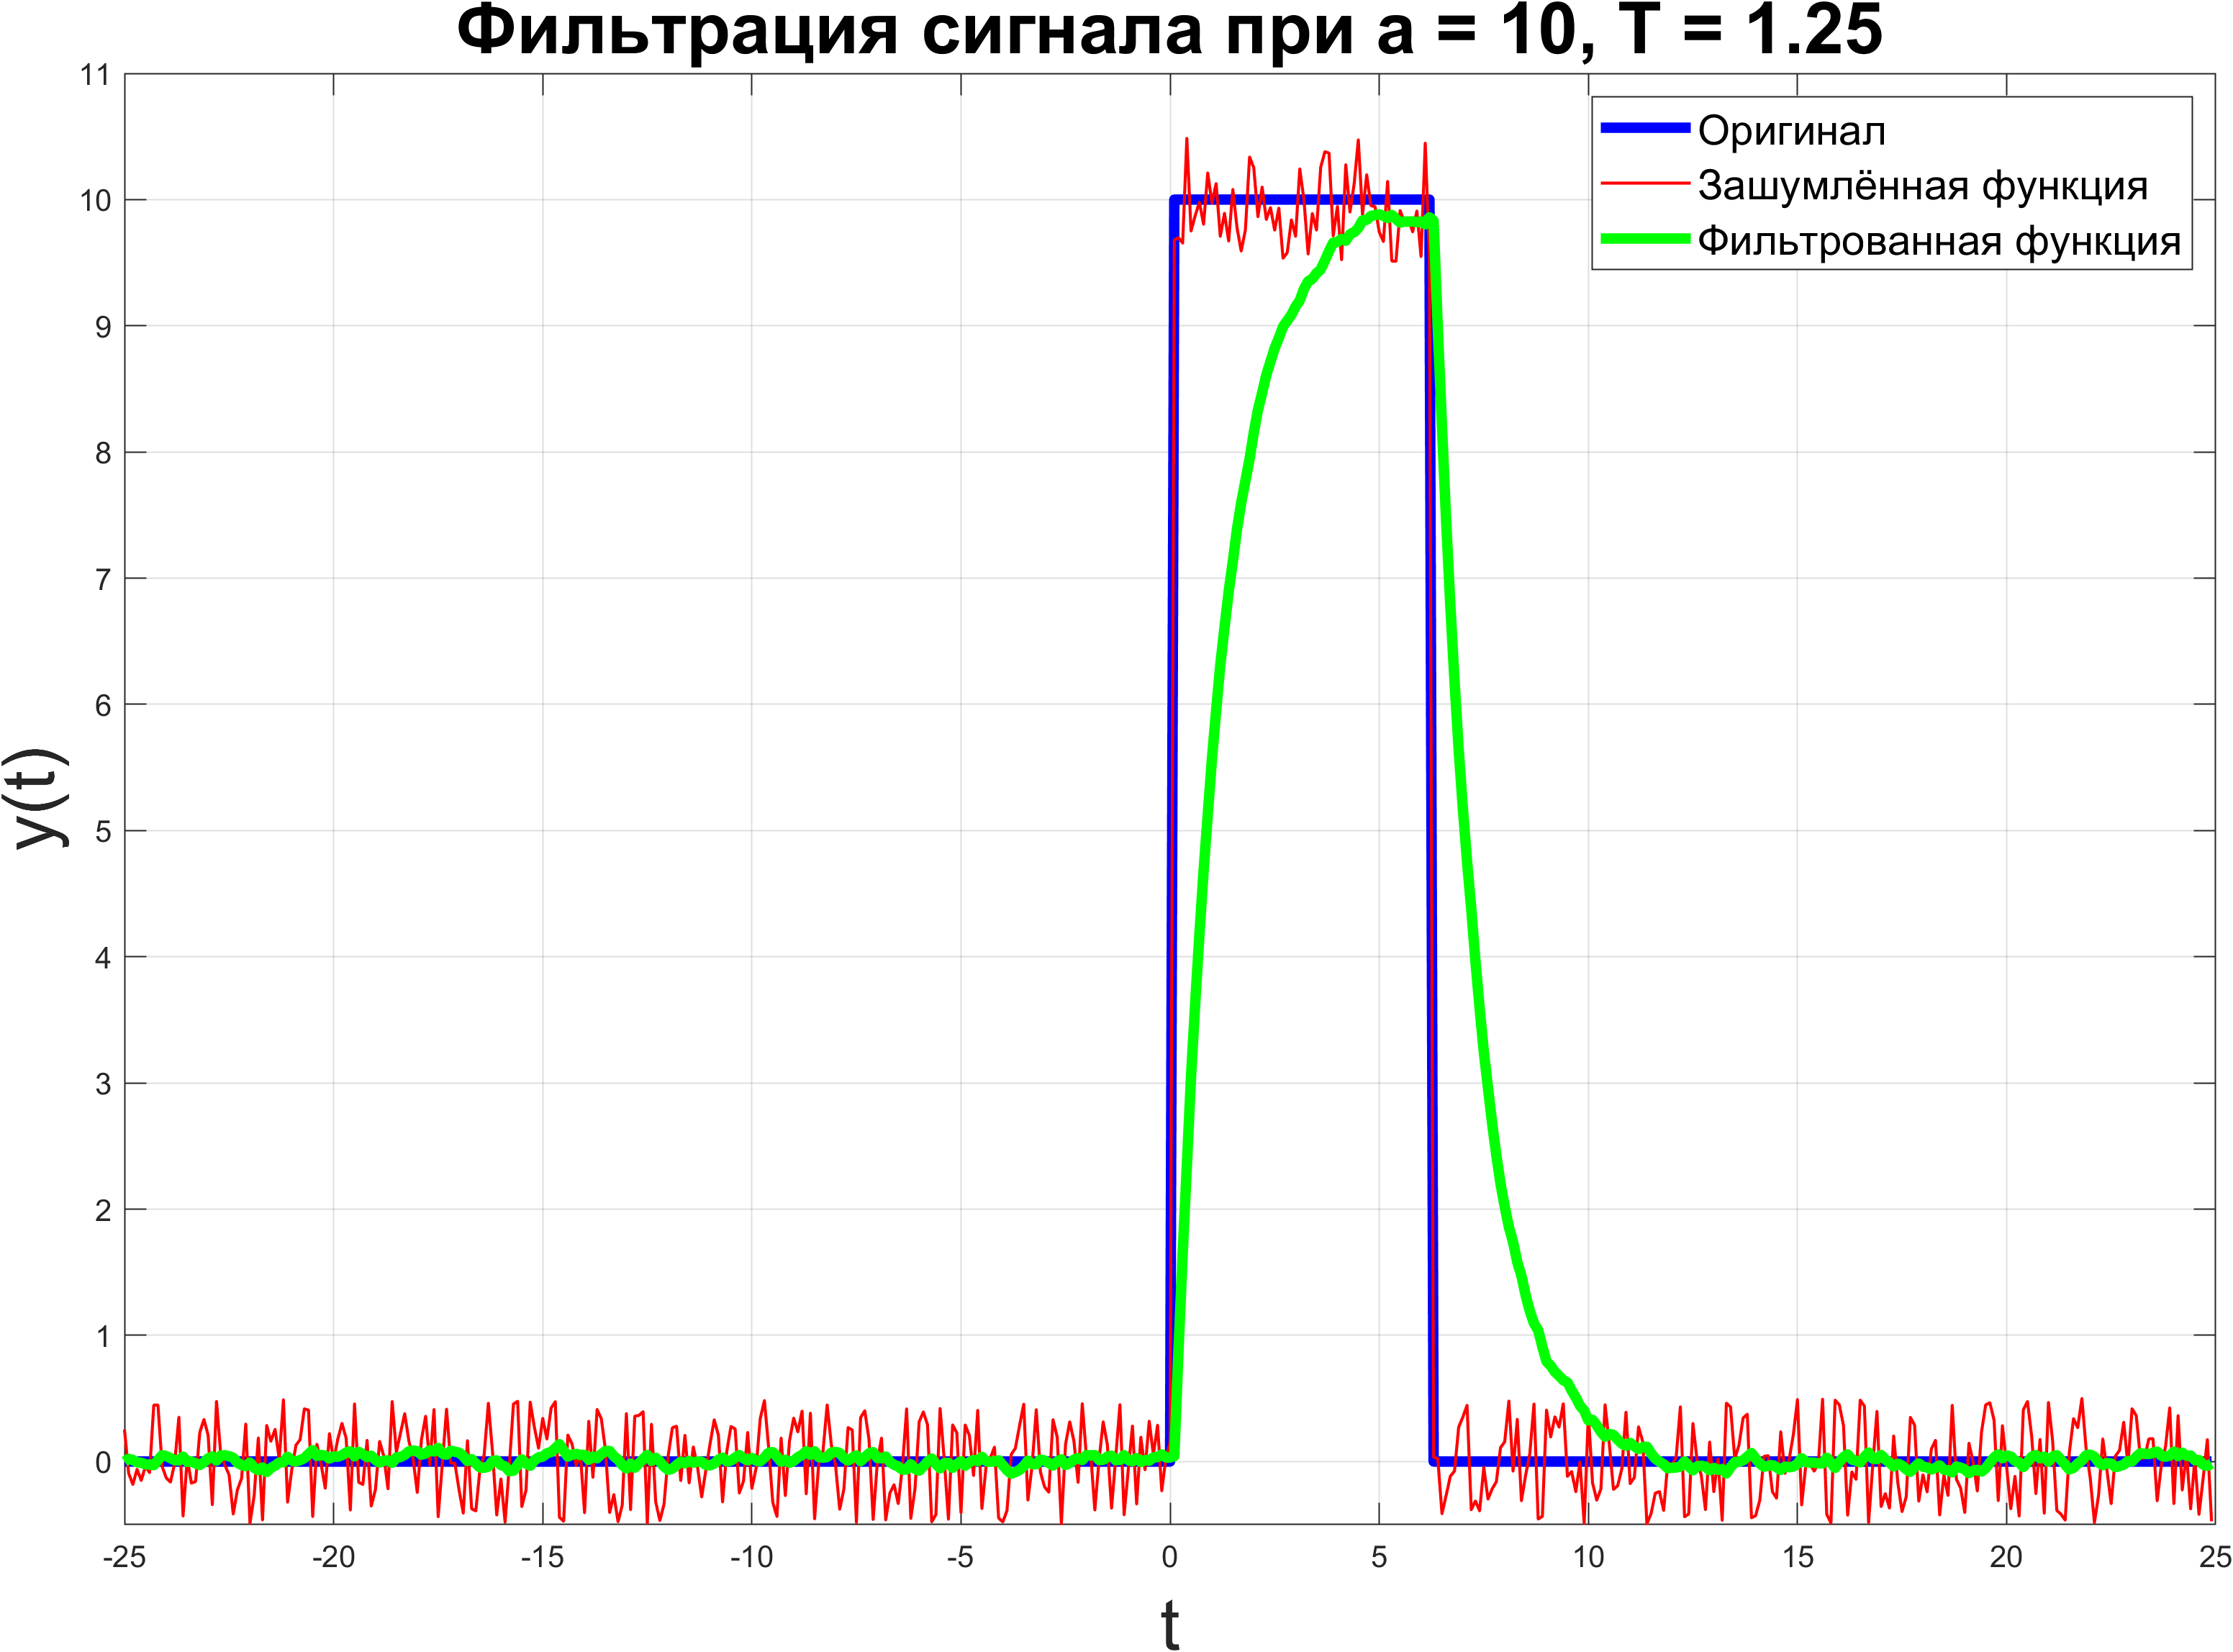
\includegraphics[width=0.92\textwidth, keepaspectratio]{images/filter_a_10.png}
    \caption{Фильтрация при $a = 10.0$}
\end{figure}
\newpage
% ==========================================
% БЛОК 8: Сравнение методов при разных a
% ==========================================
\subsection{Сравнение методов фильтрации (параметр $a$)}


\begin{figure}[H]
    \centering
    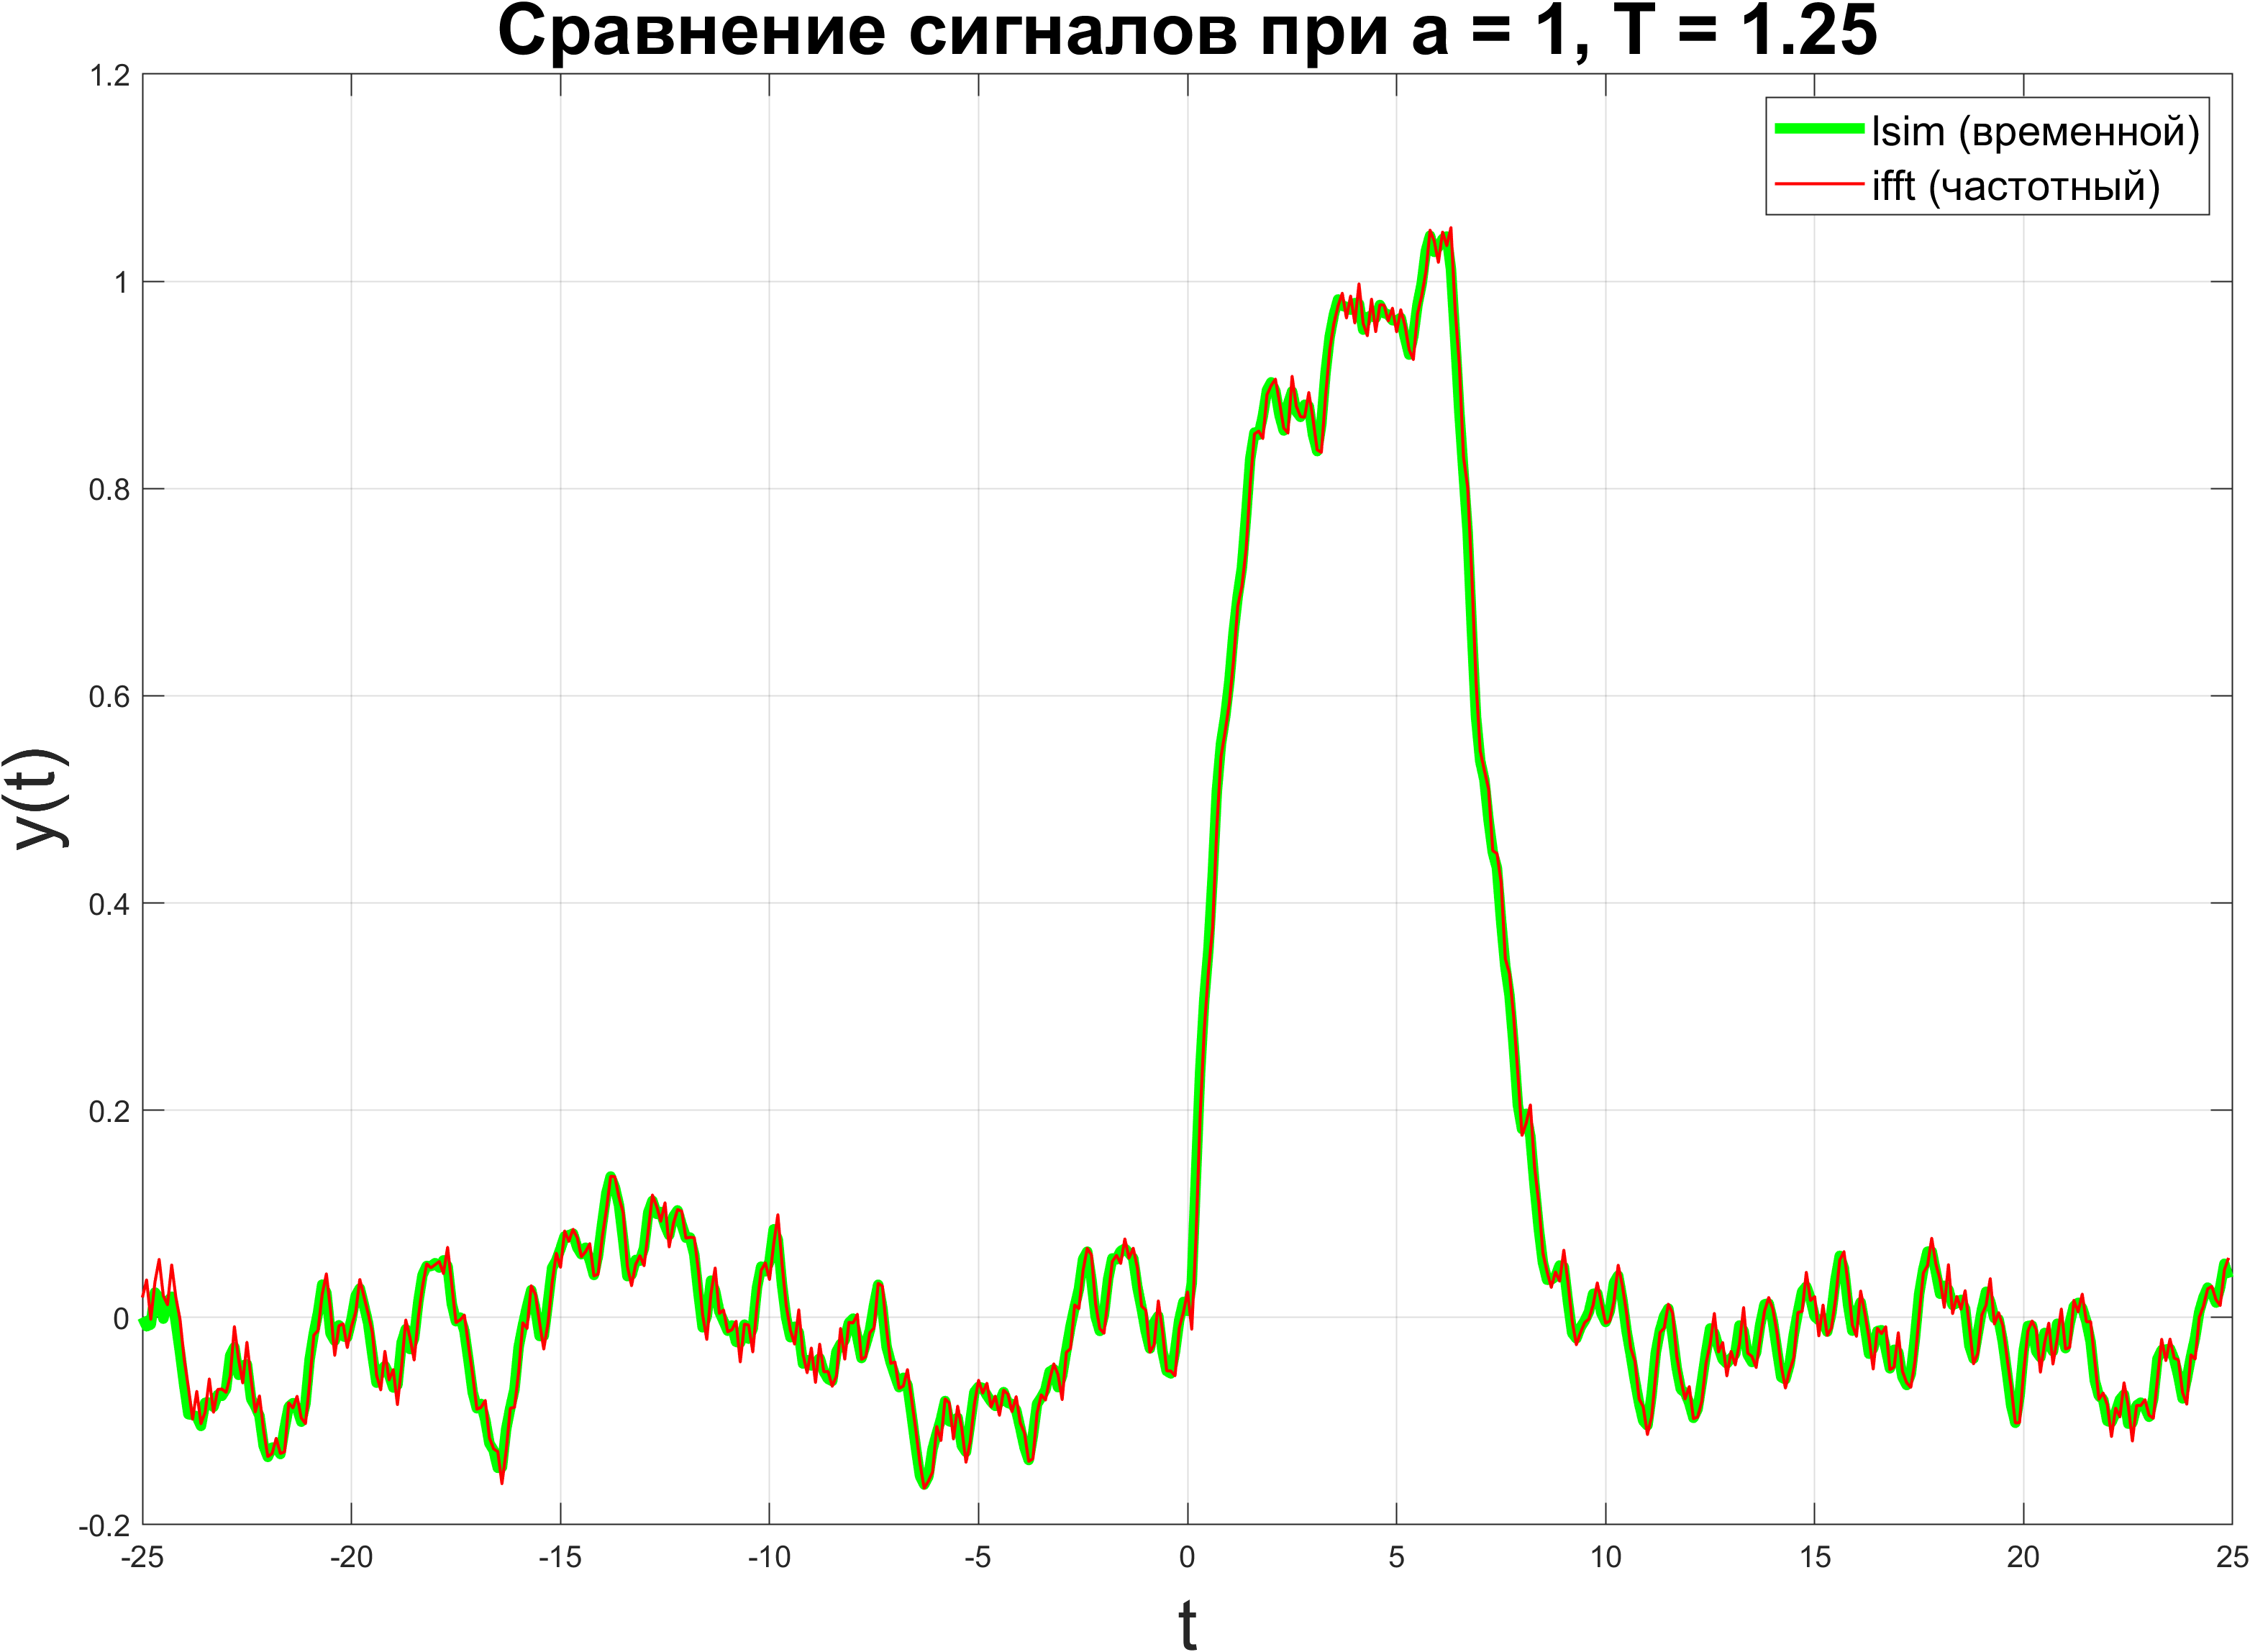
\includegraphics[width=0.85\textwidth, keepaspectratio]{images/filter_transf_a_1.png}
    \caption{Сравнение методов при $a = 1.0$}
\end{figure}
\begin{figure}[H]
    \centering
    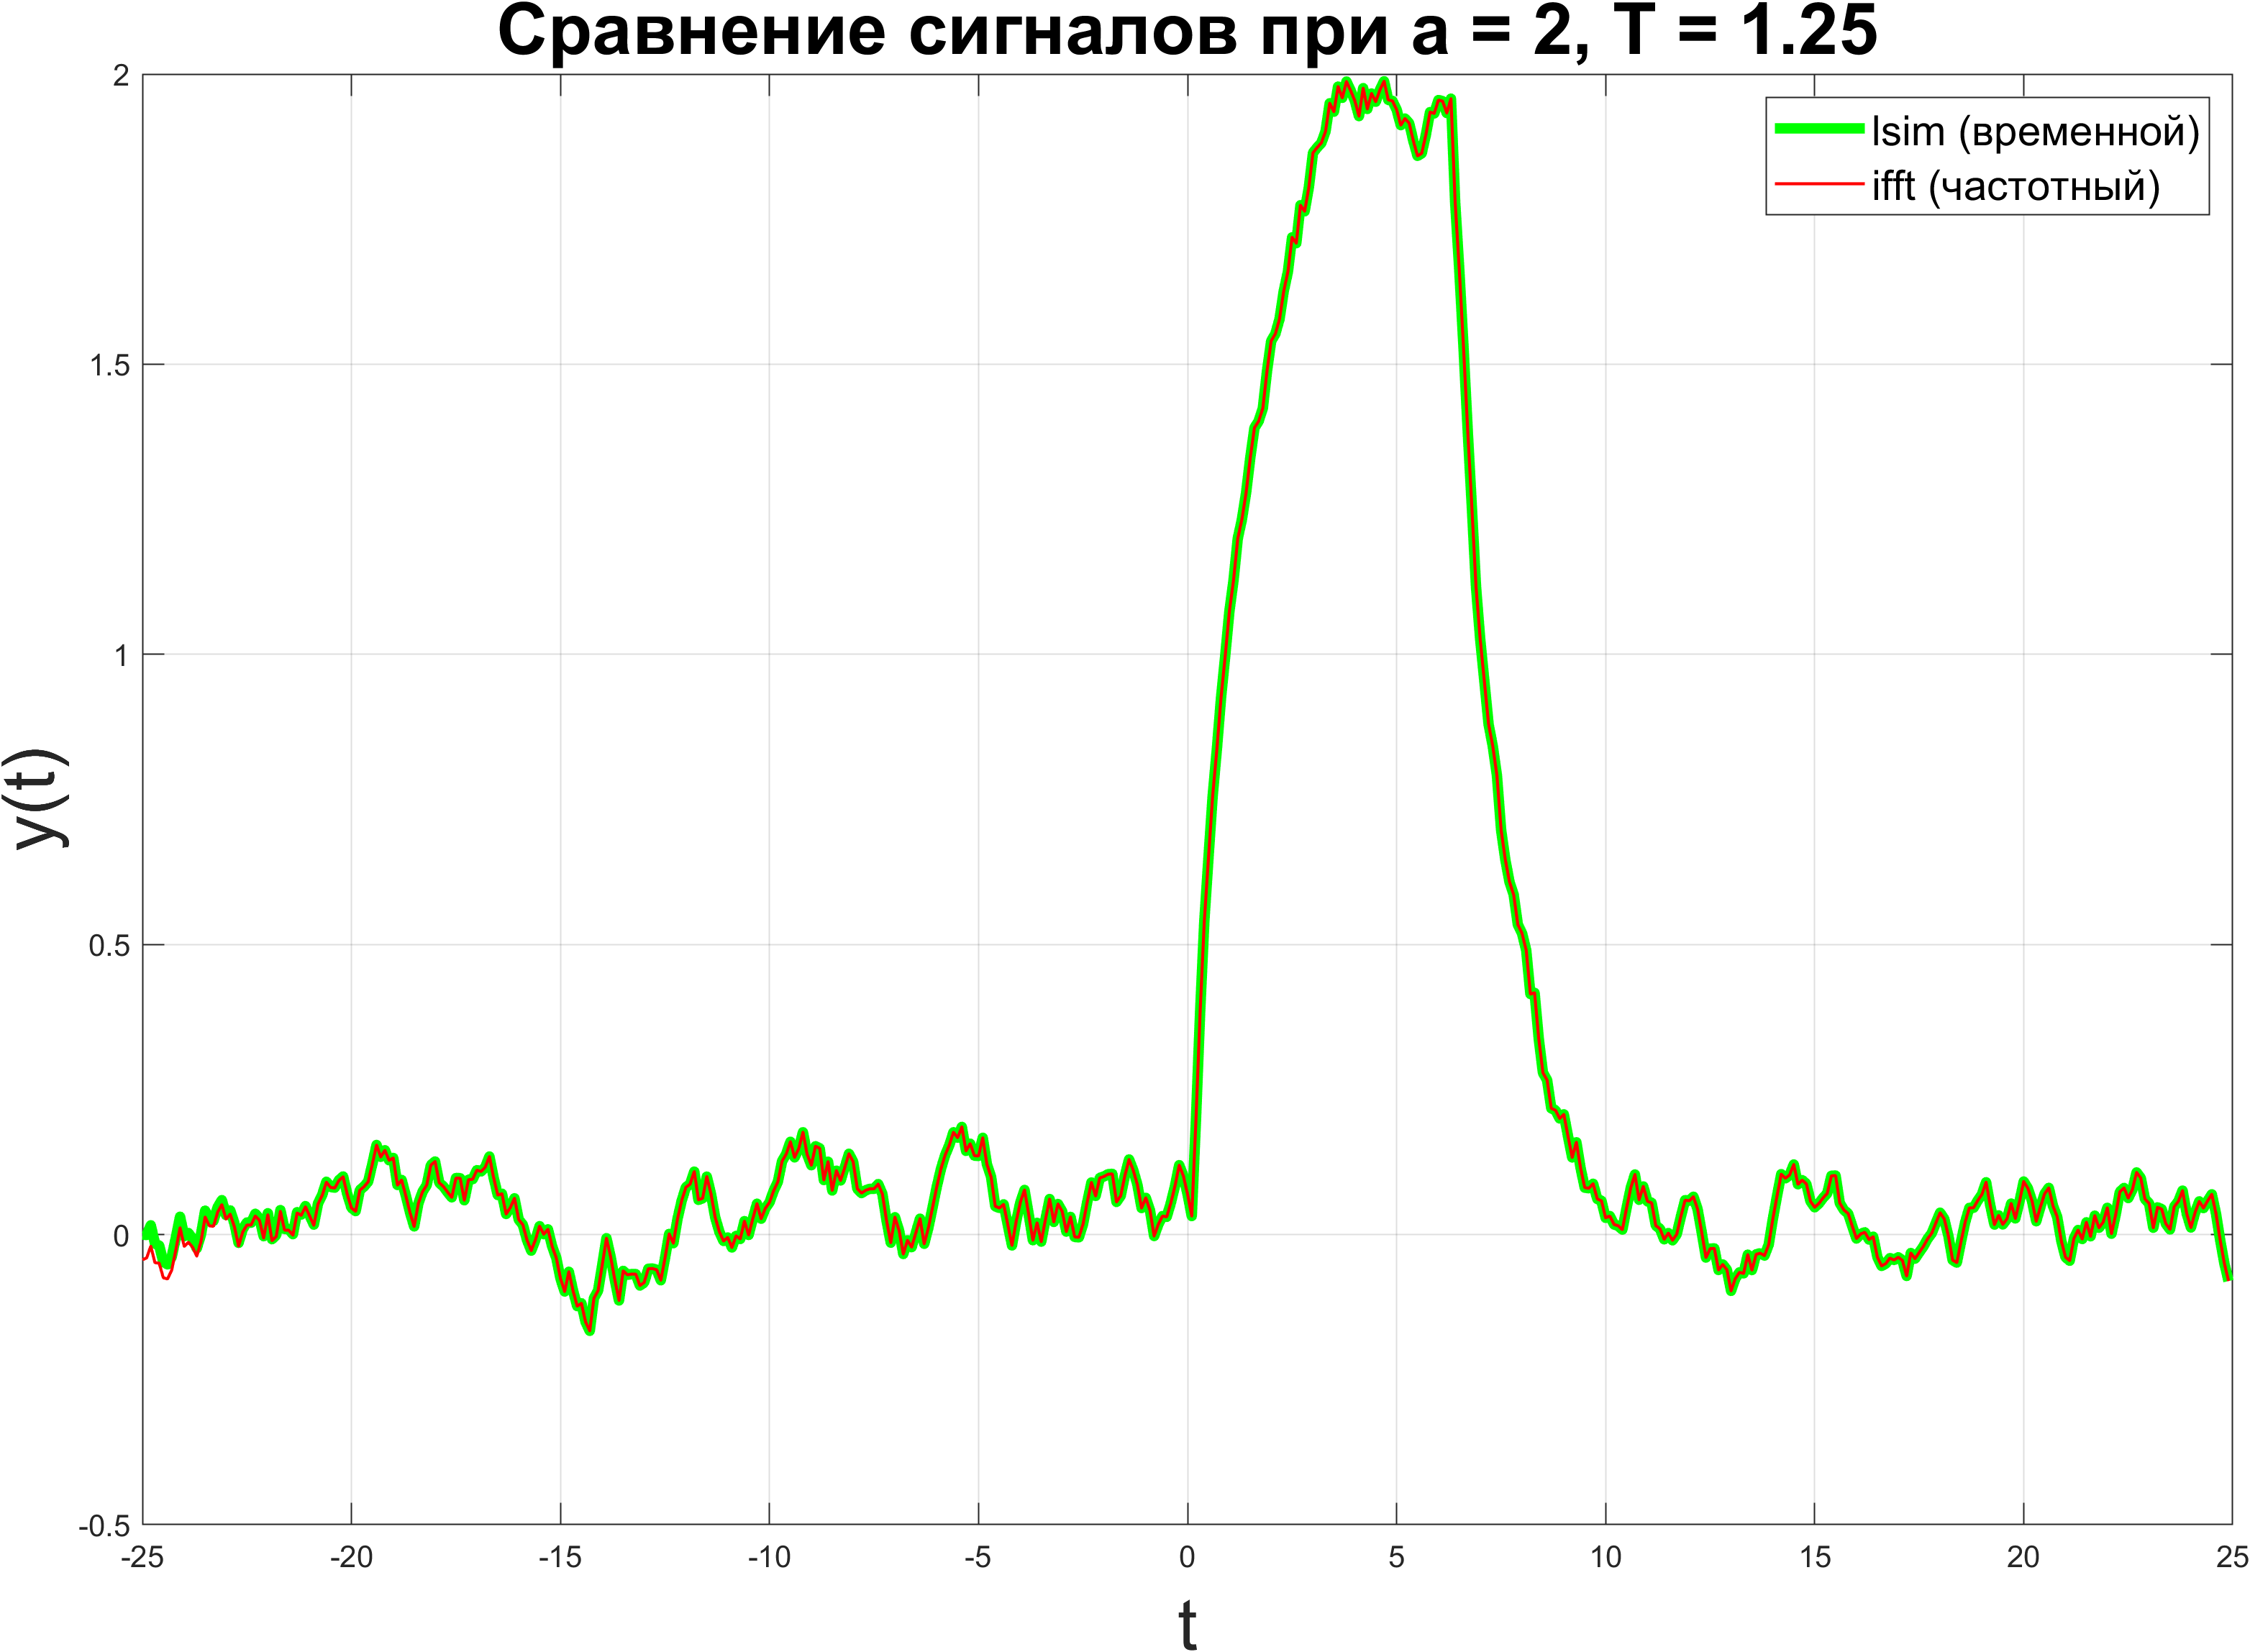
\includegraphics[width=0.85\textwidth, keepaspectratio]{images/filter_transf_a_2.png}
    \caption{Сравнение методов при $a = 2.0$}
\end{figure}
\newpage

\begin{figure}[H]
    \centering
    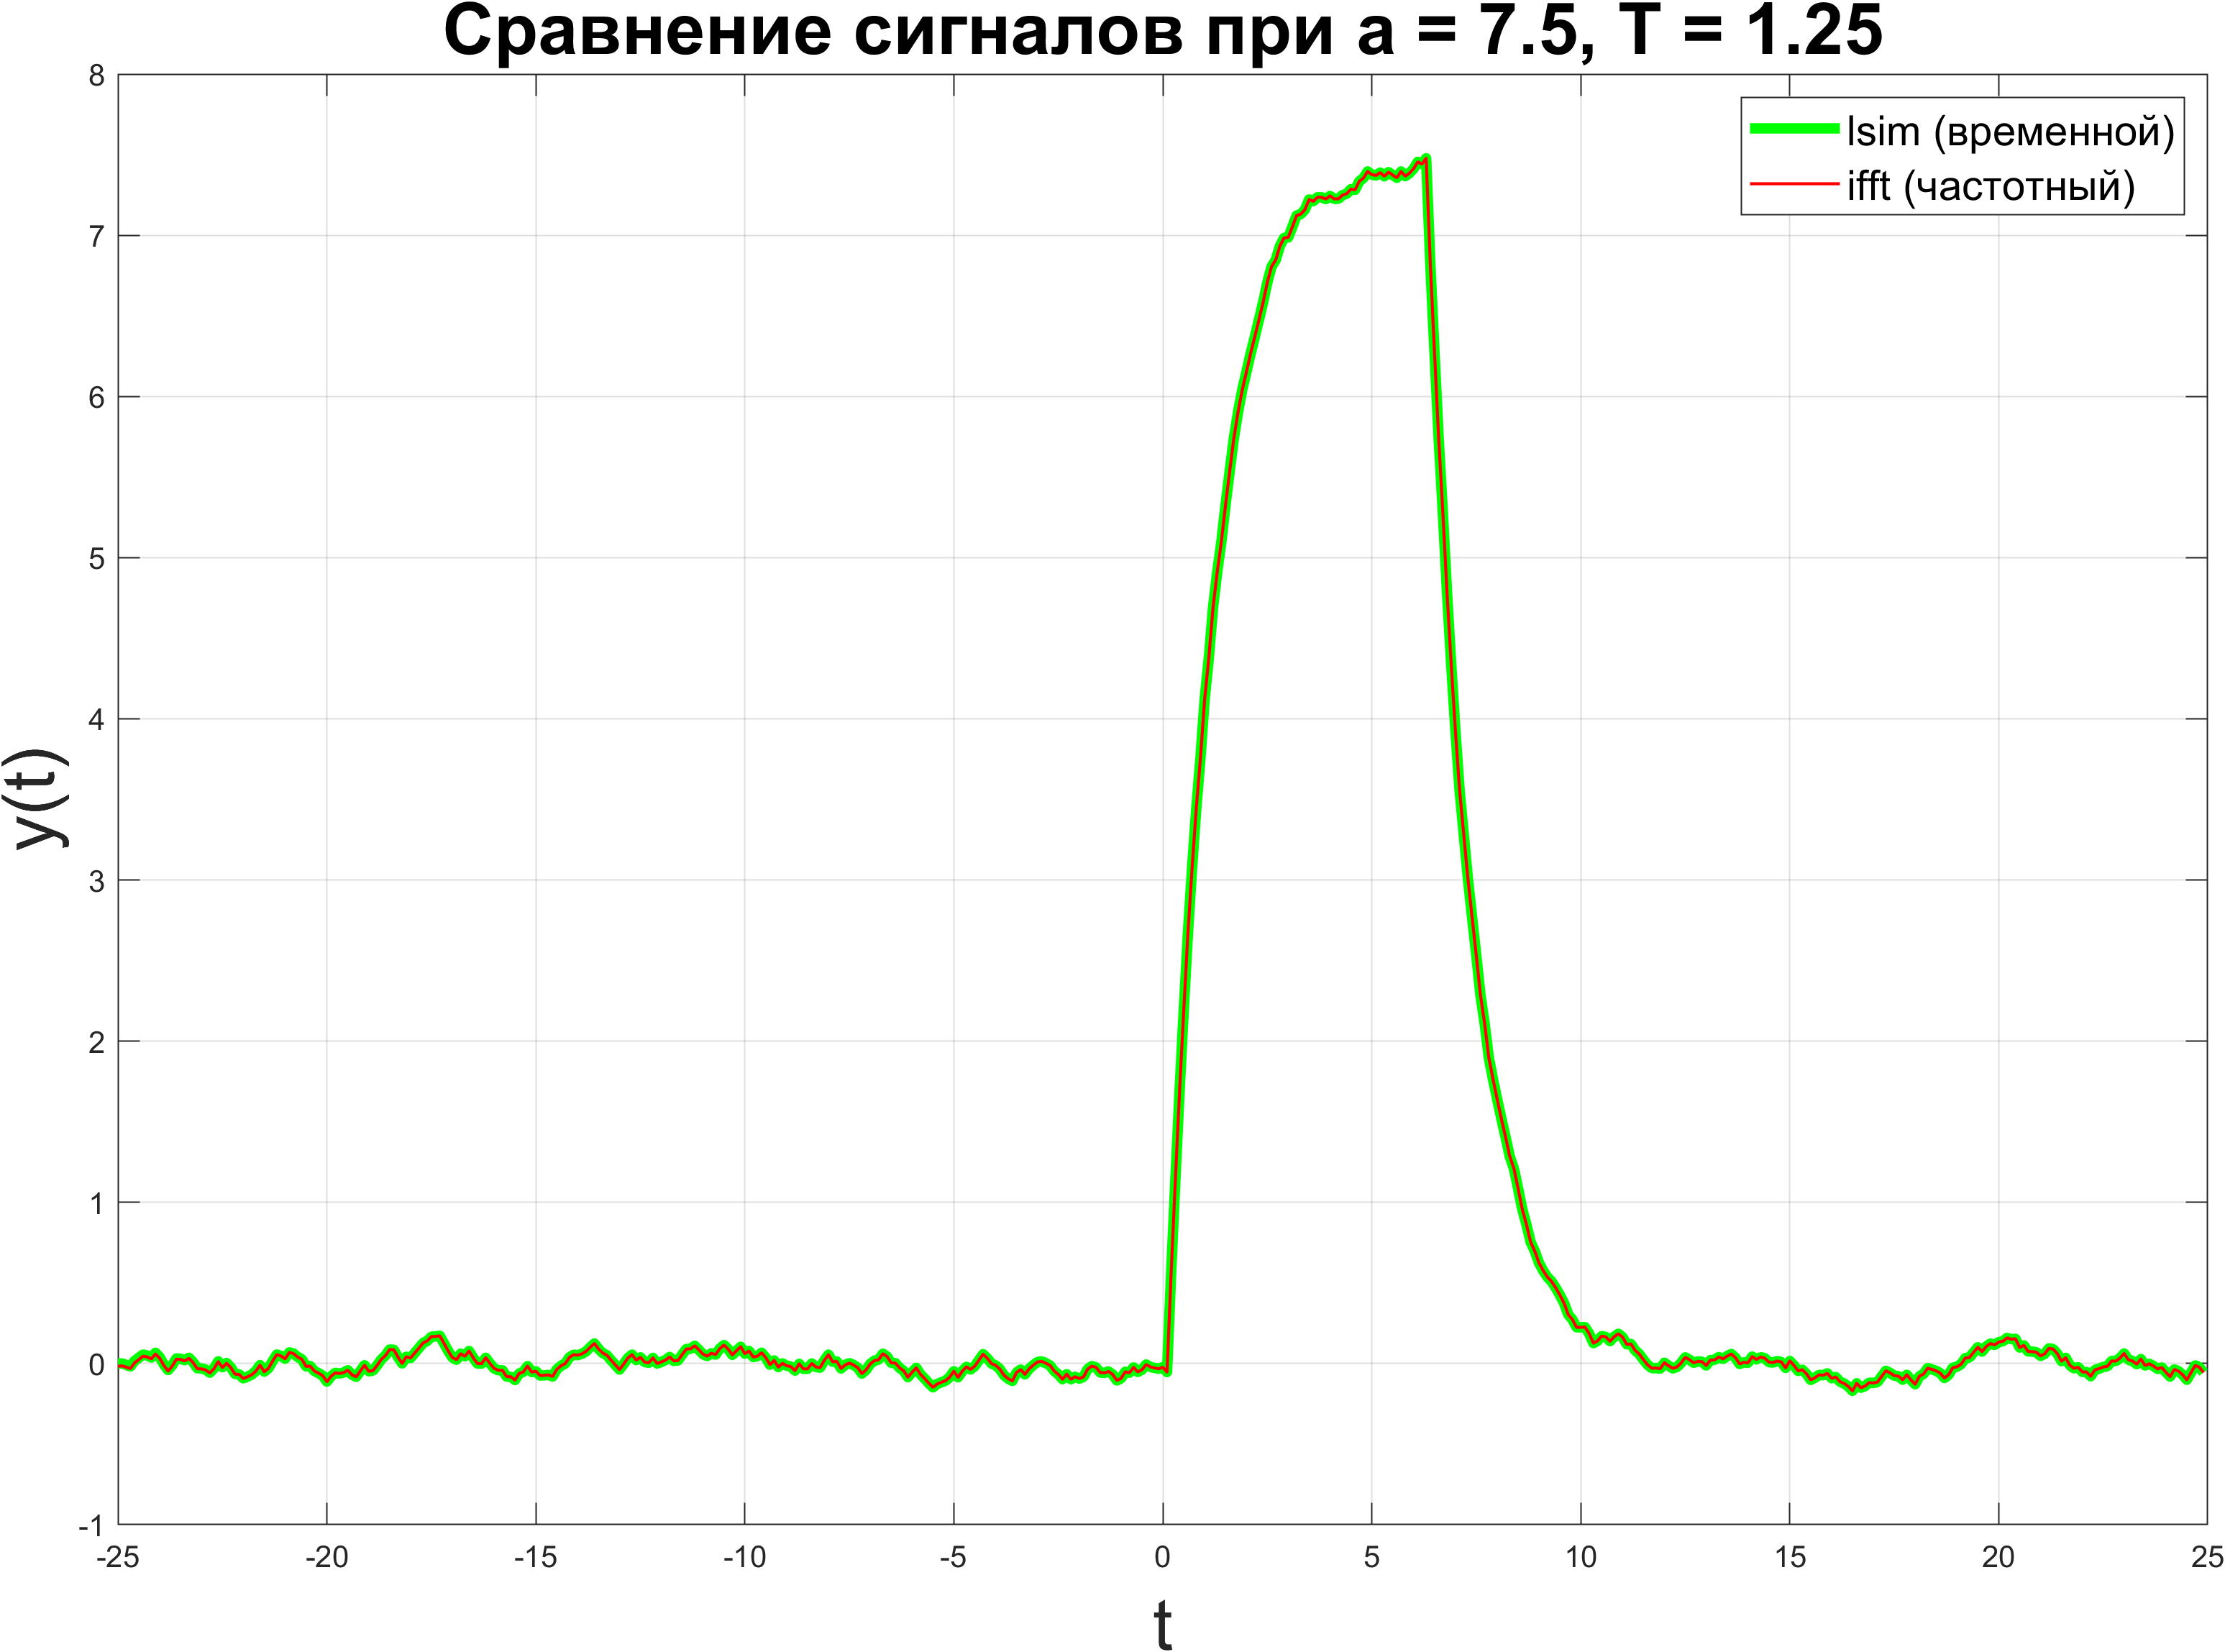
\includegraphics[width=0.92\textwidth, keepaspectratio]{images/filter_transf_a_7.5.png}
    \caption{Сравнение методов при $a = 7.5$}
\end{figure}
\begin{figure}[H]
    \centering
    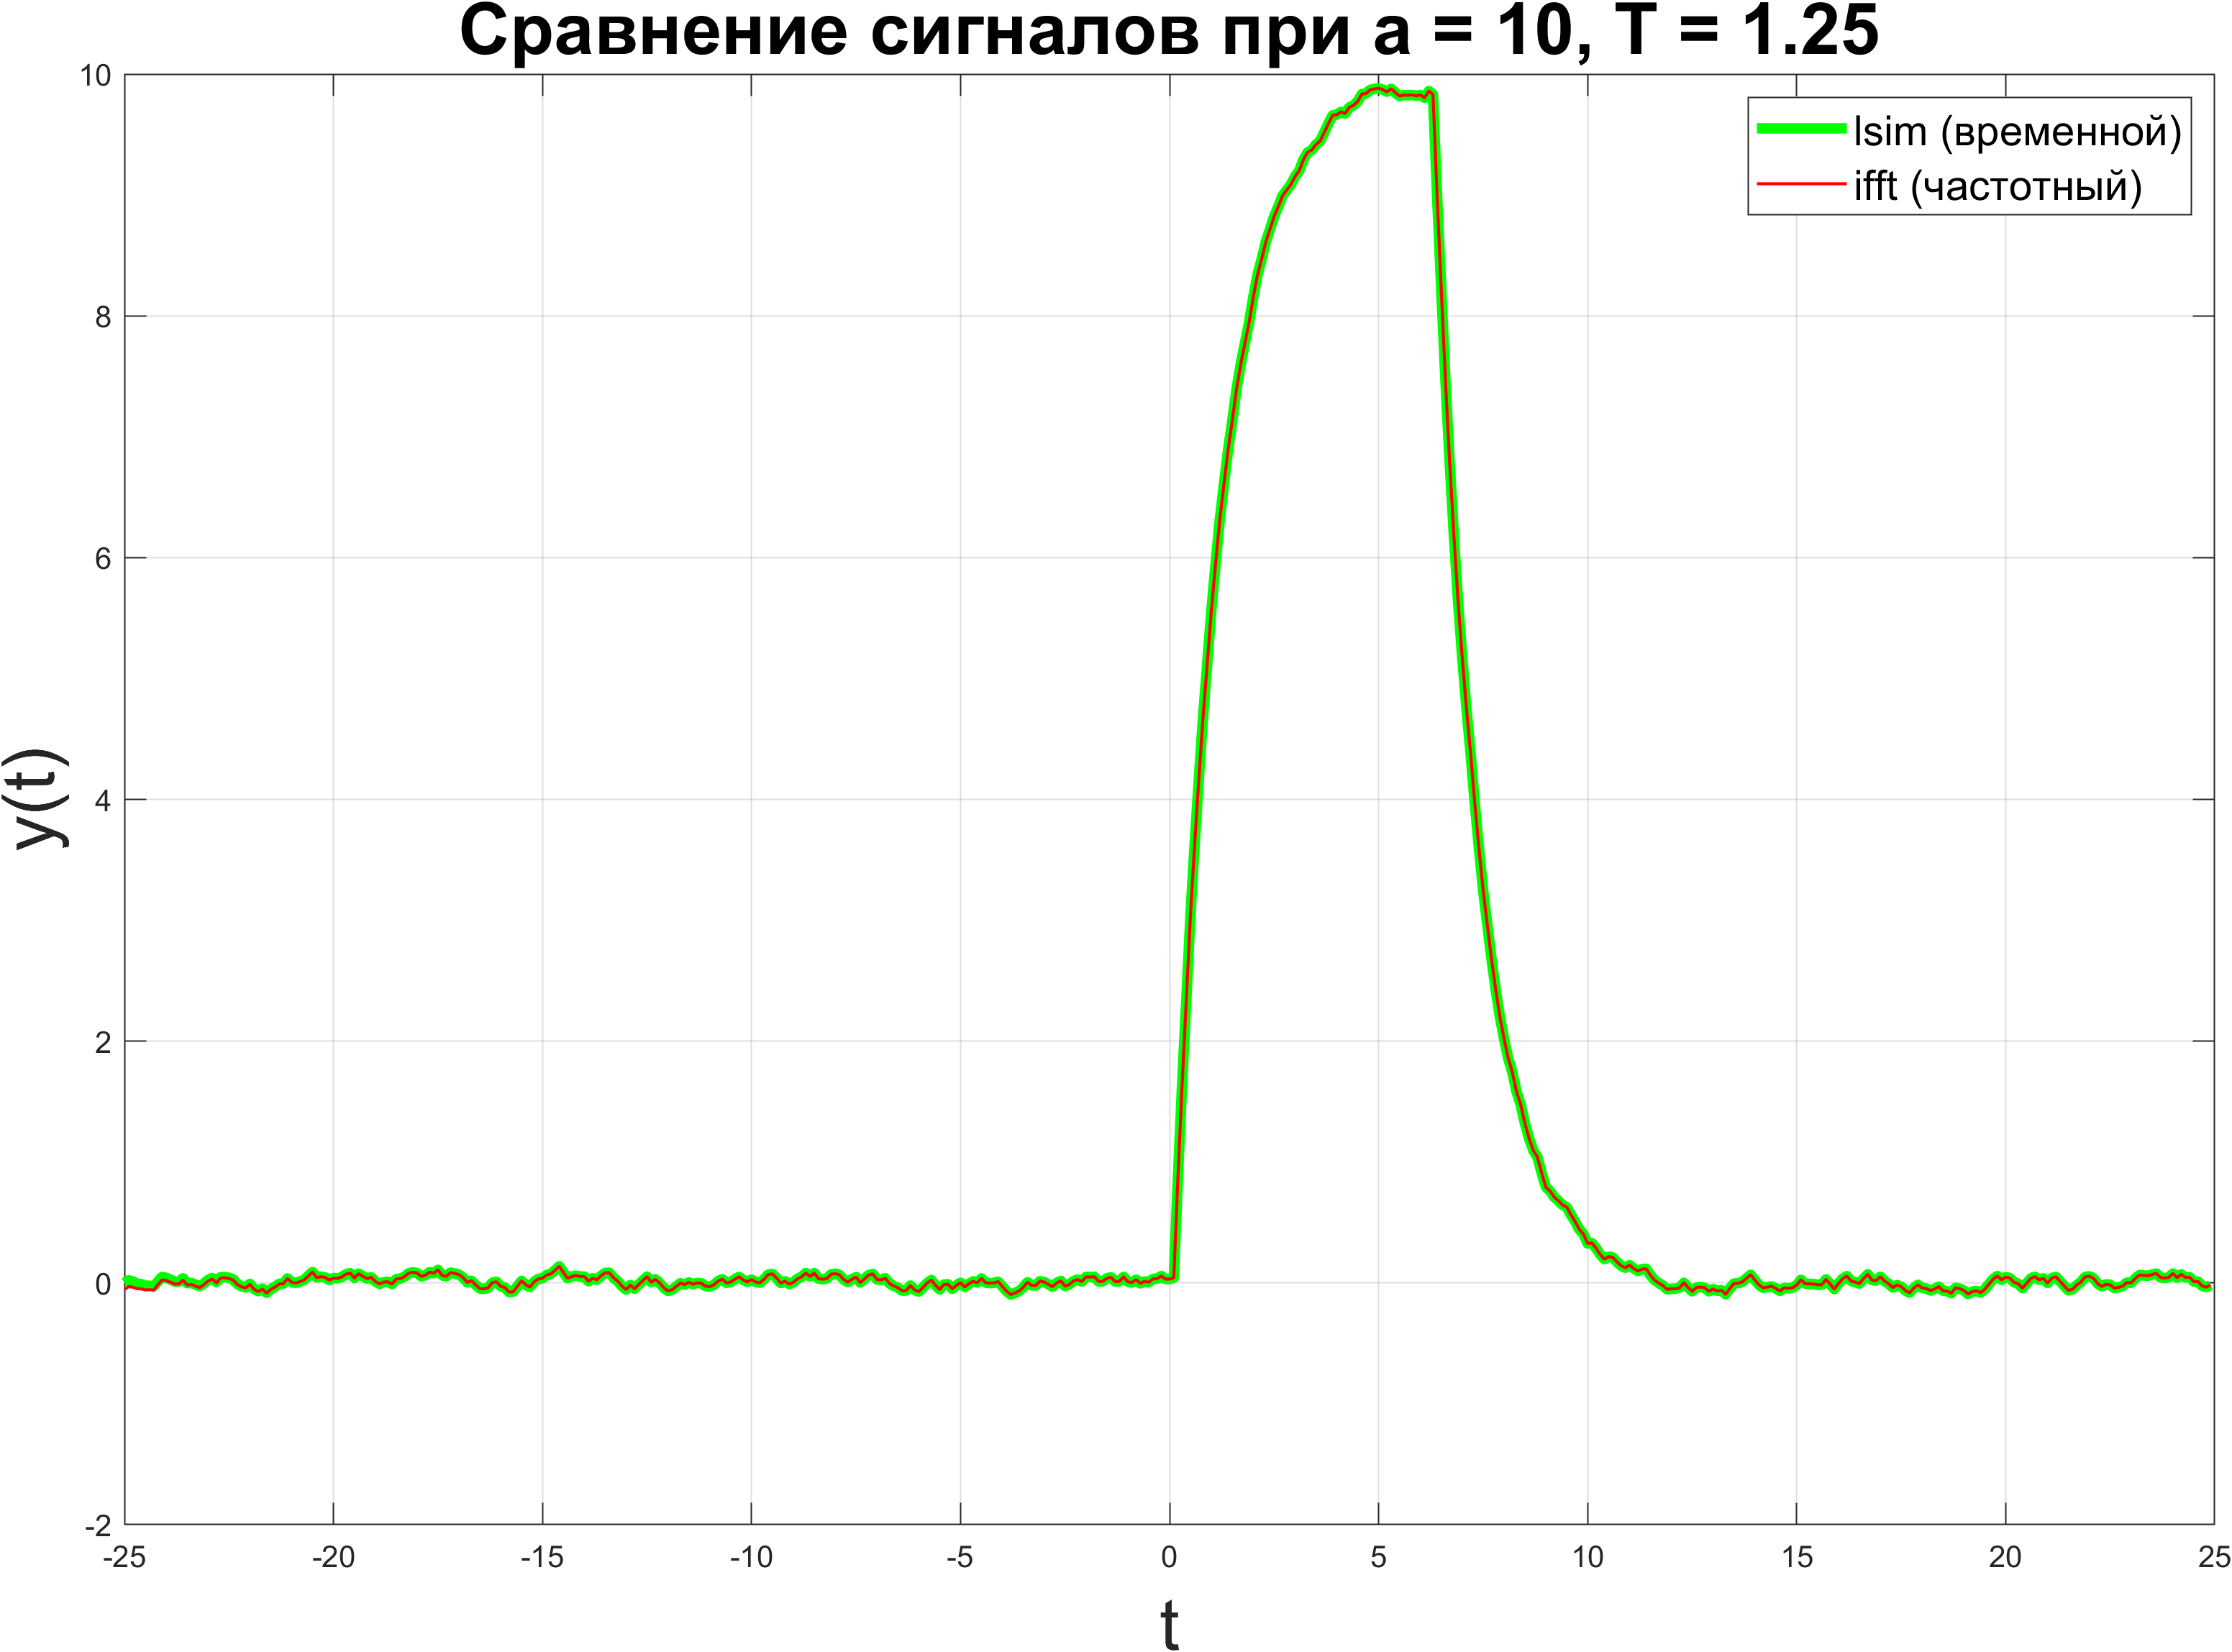
\includegraphics[width=0.92\textwidth, keepaspectratio]{images/filter_transf_a_10.png}
    \caption{Сравнение методов при $a = 10.0$}
\end{figure}
\newpage
% ==========================================
% БЛОК 9: Фурье-образы (сигналы) при разных a
% ==========================================
\subsection{Фурье-образы $g$, $y$, $y_{fil}$ (параметр $a$)}


\begin{figure}[H]
    \centering
    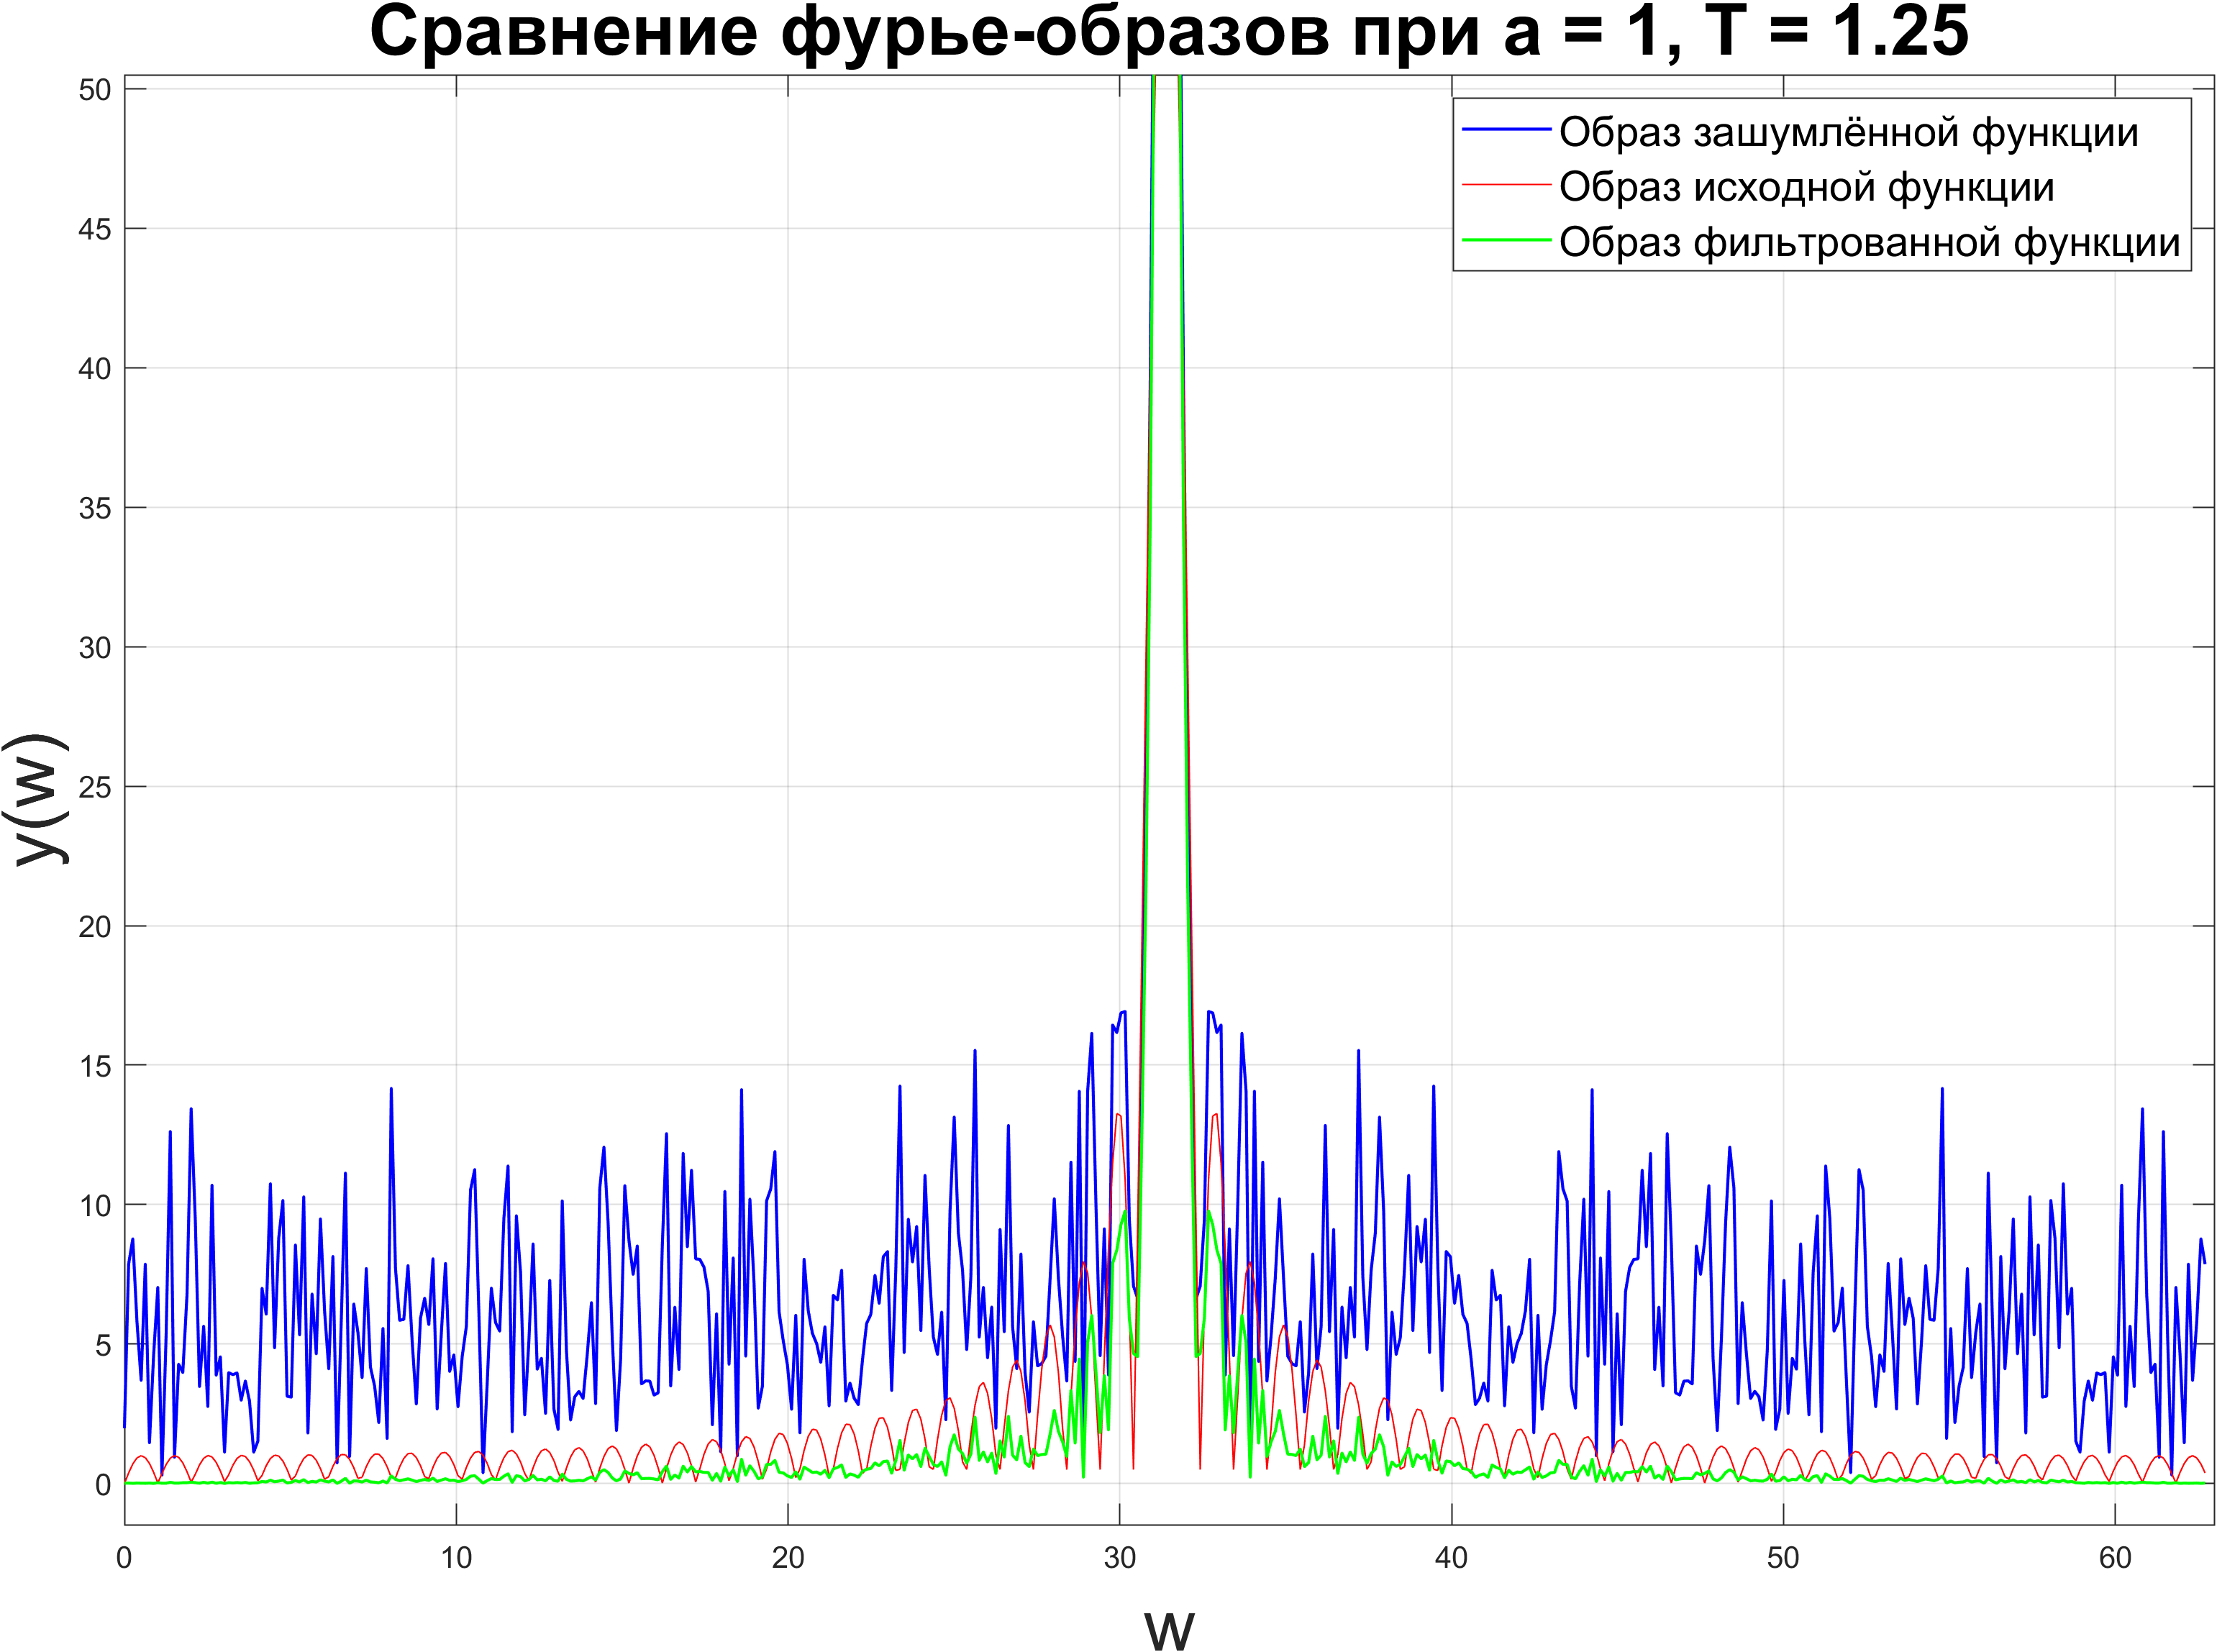
\includegraphics[width=0.85\textwidth, keepaspectratio]{images/fur_imgs_g_a_1.png}
    \caption{Фурье-образы при $a = 1.0$}
\end{figure}
\begin{figure}[H]
    \centering
    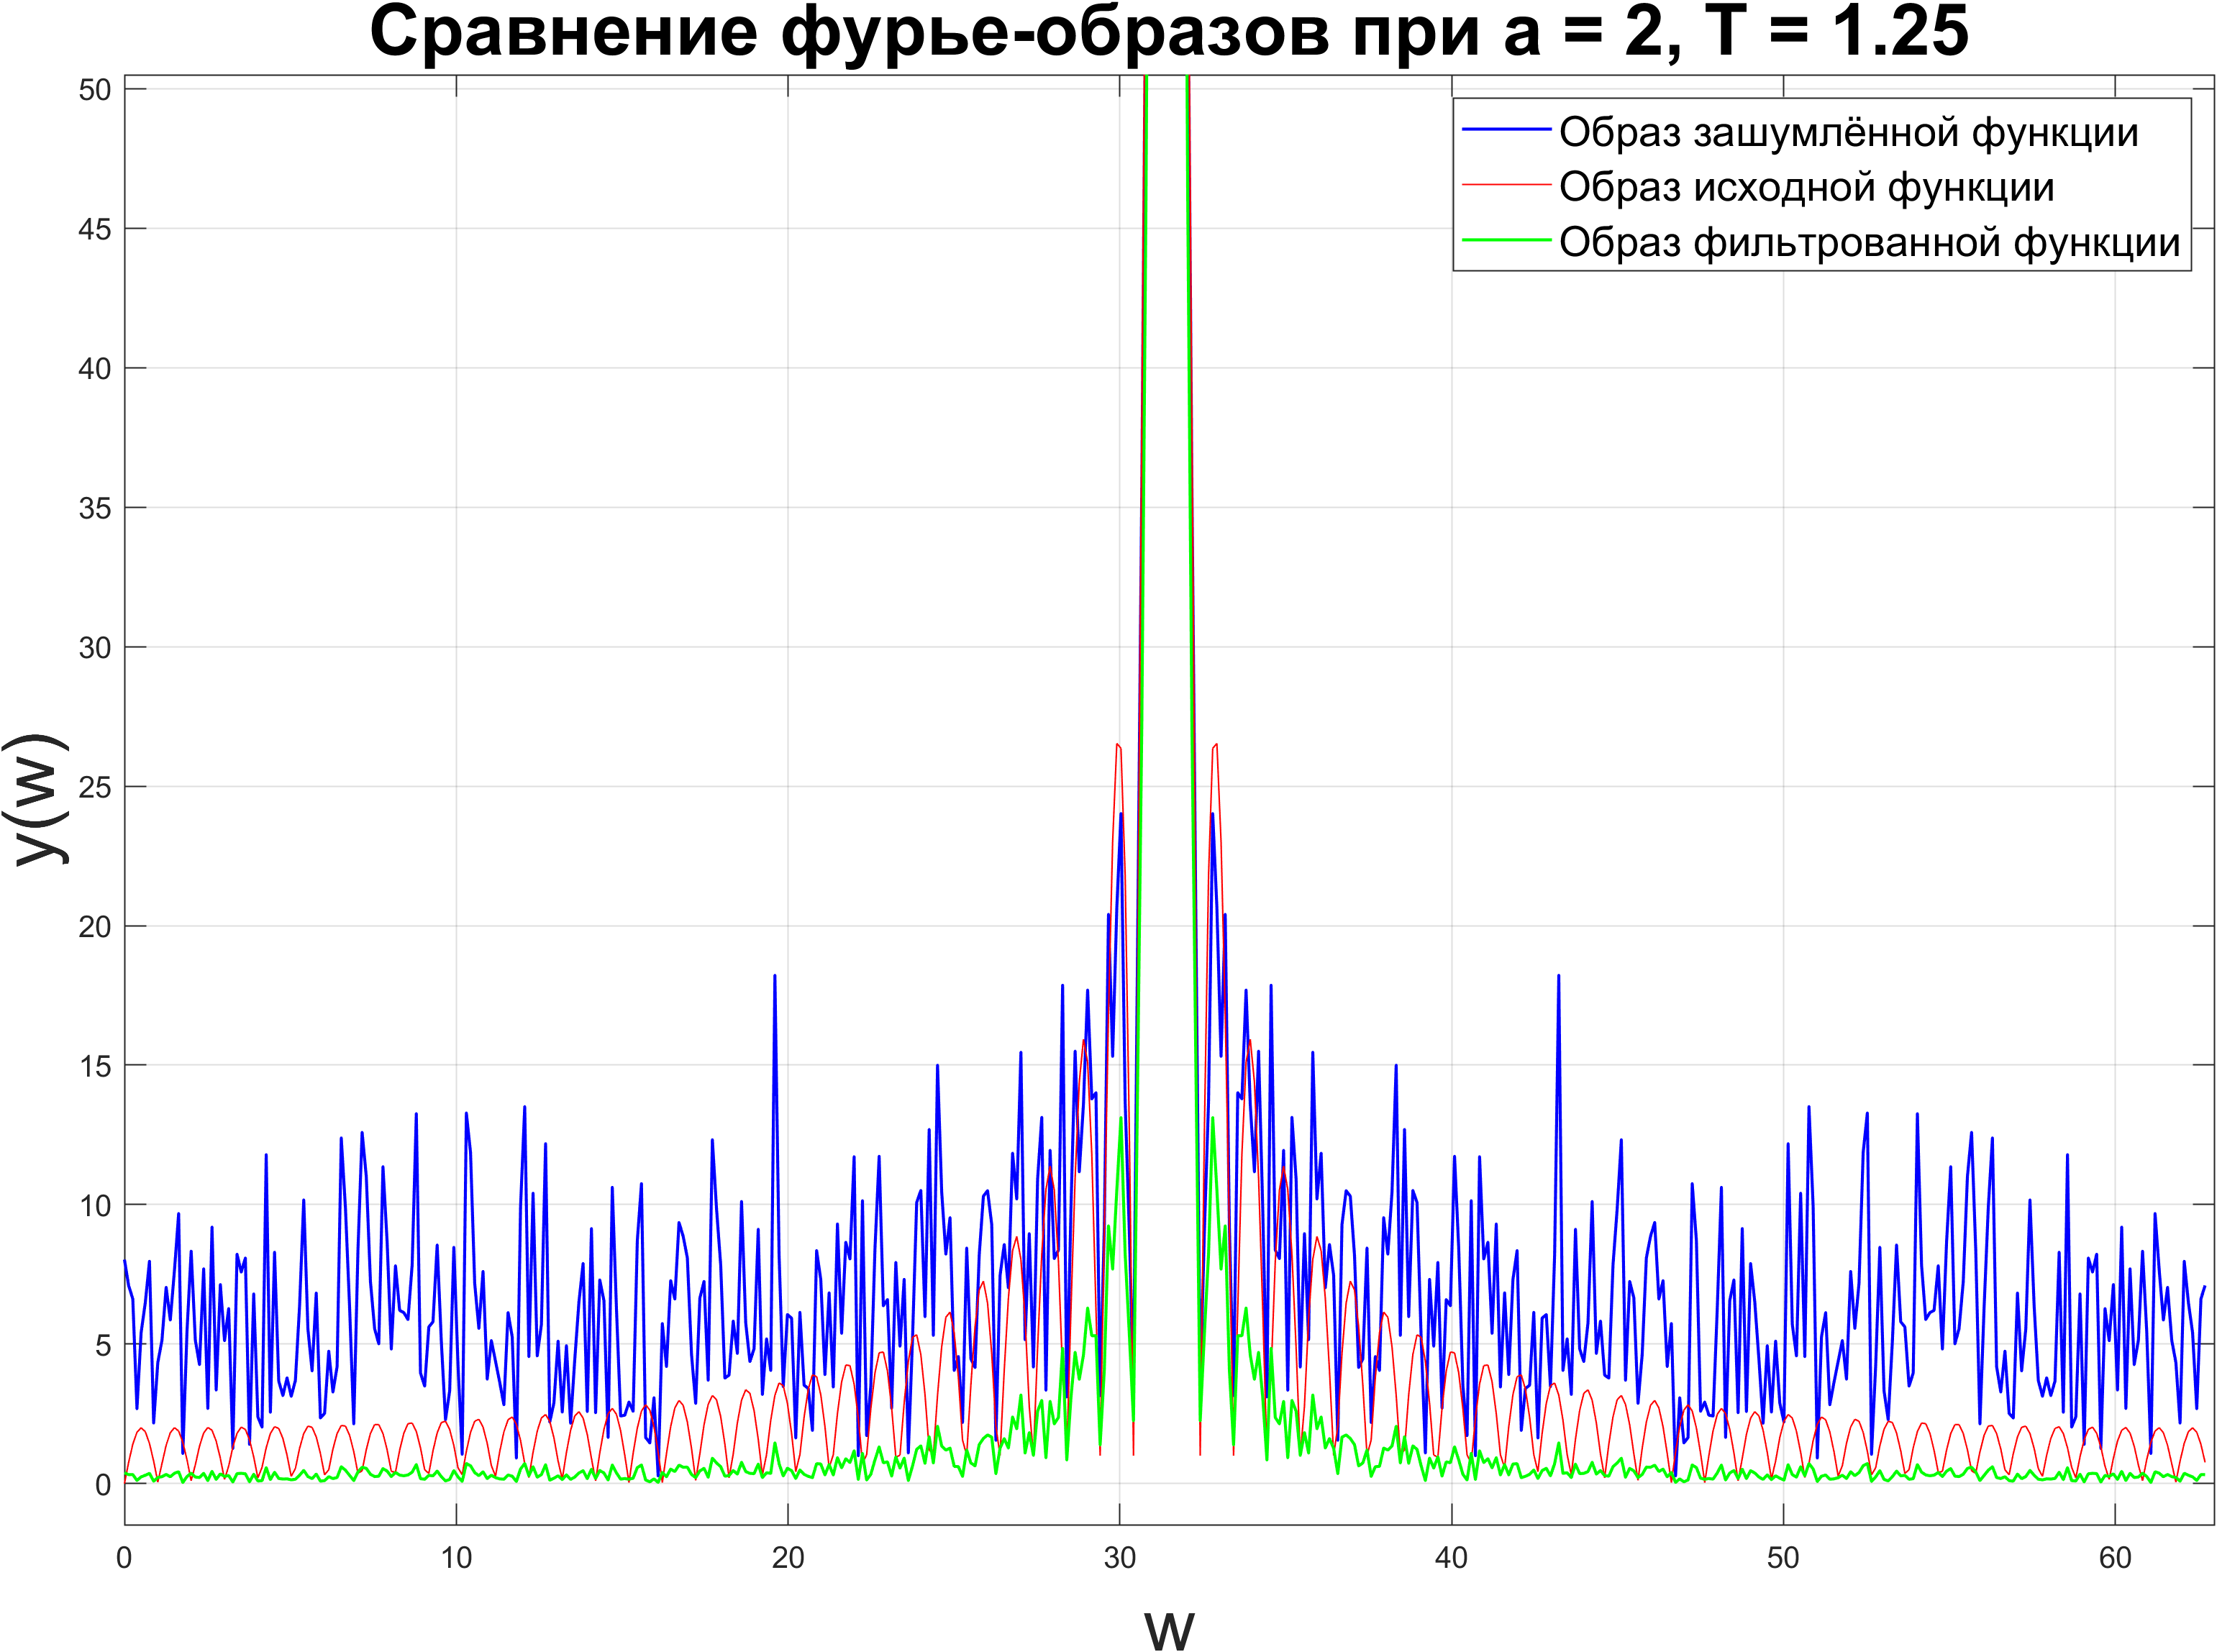
\includegraphics[width=0.85\textwidth, keepaspectratio]{images/fur_imgs_g_a_2.png}
    \caption{Фурье-образы при $a = 2.0$}
\end{figure}
\newpage

\begin{figure}[H]
    \centering
    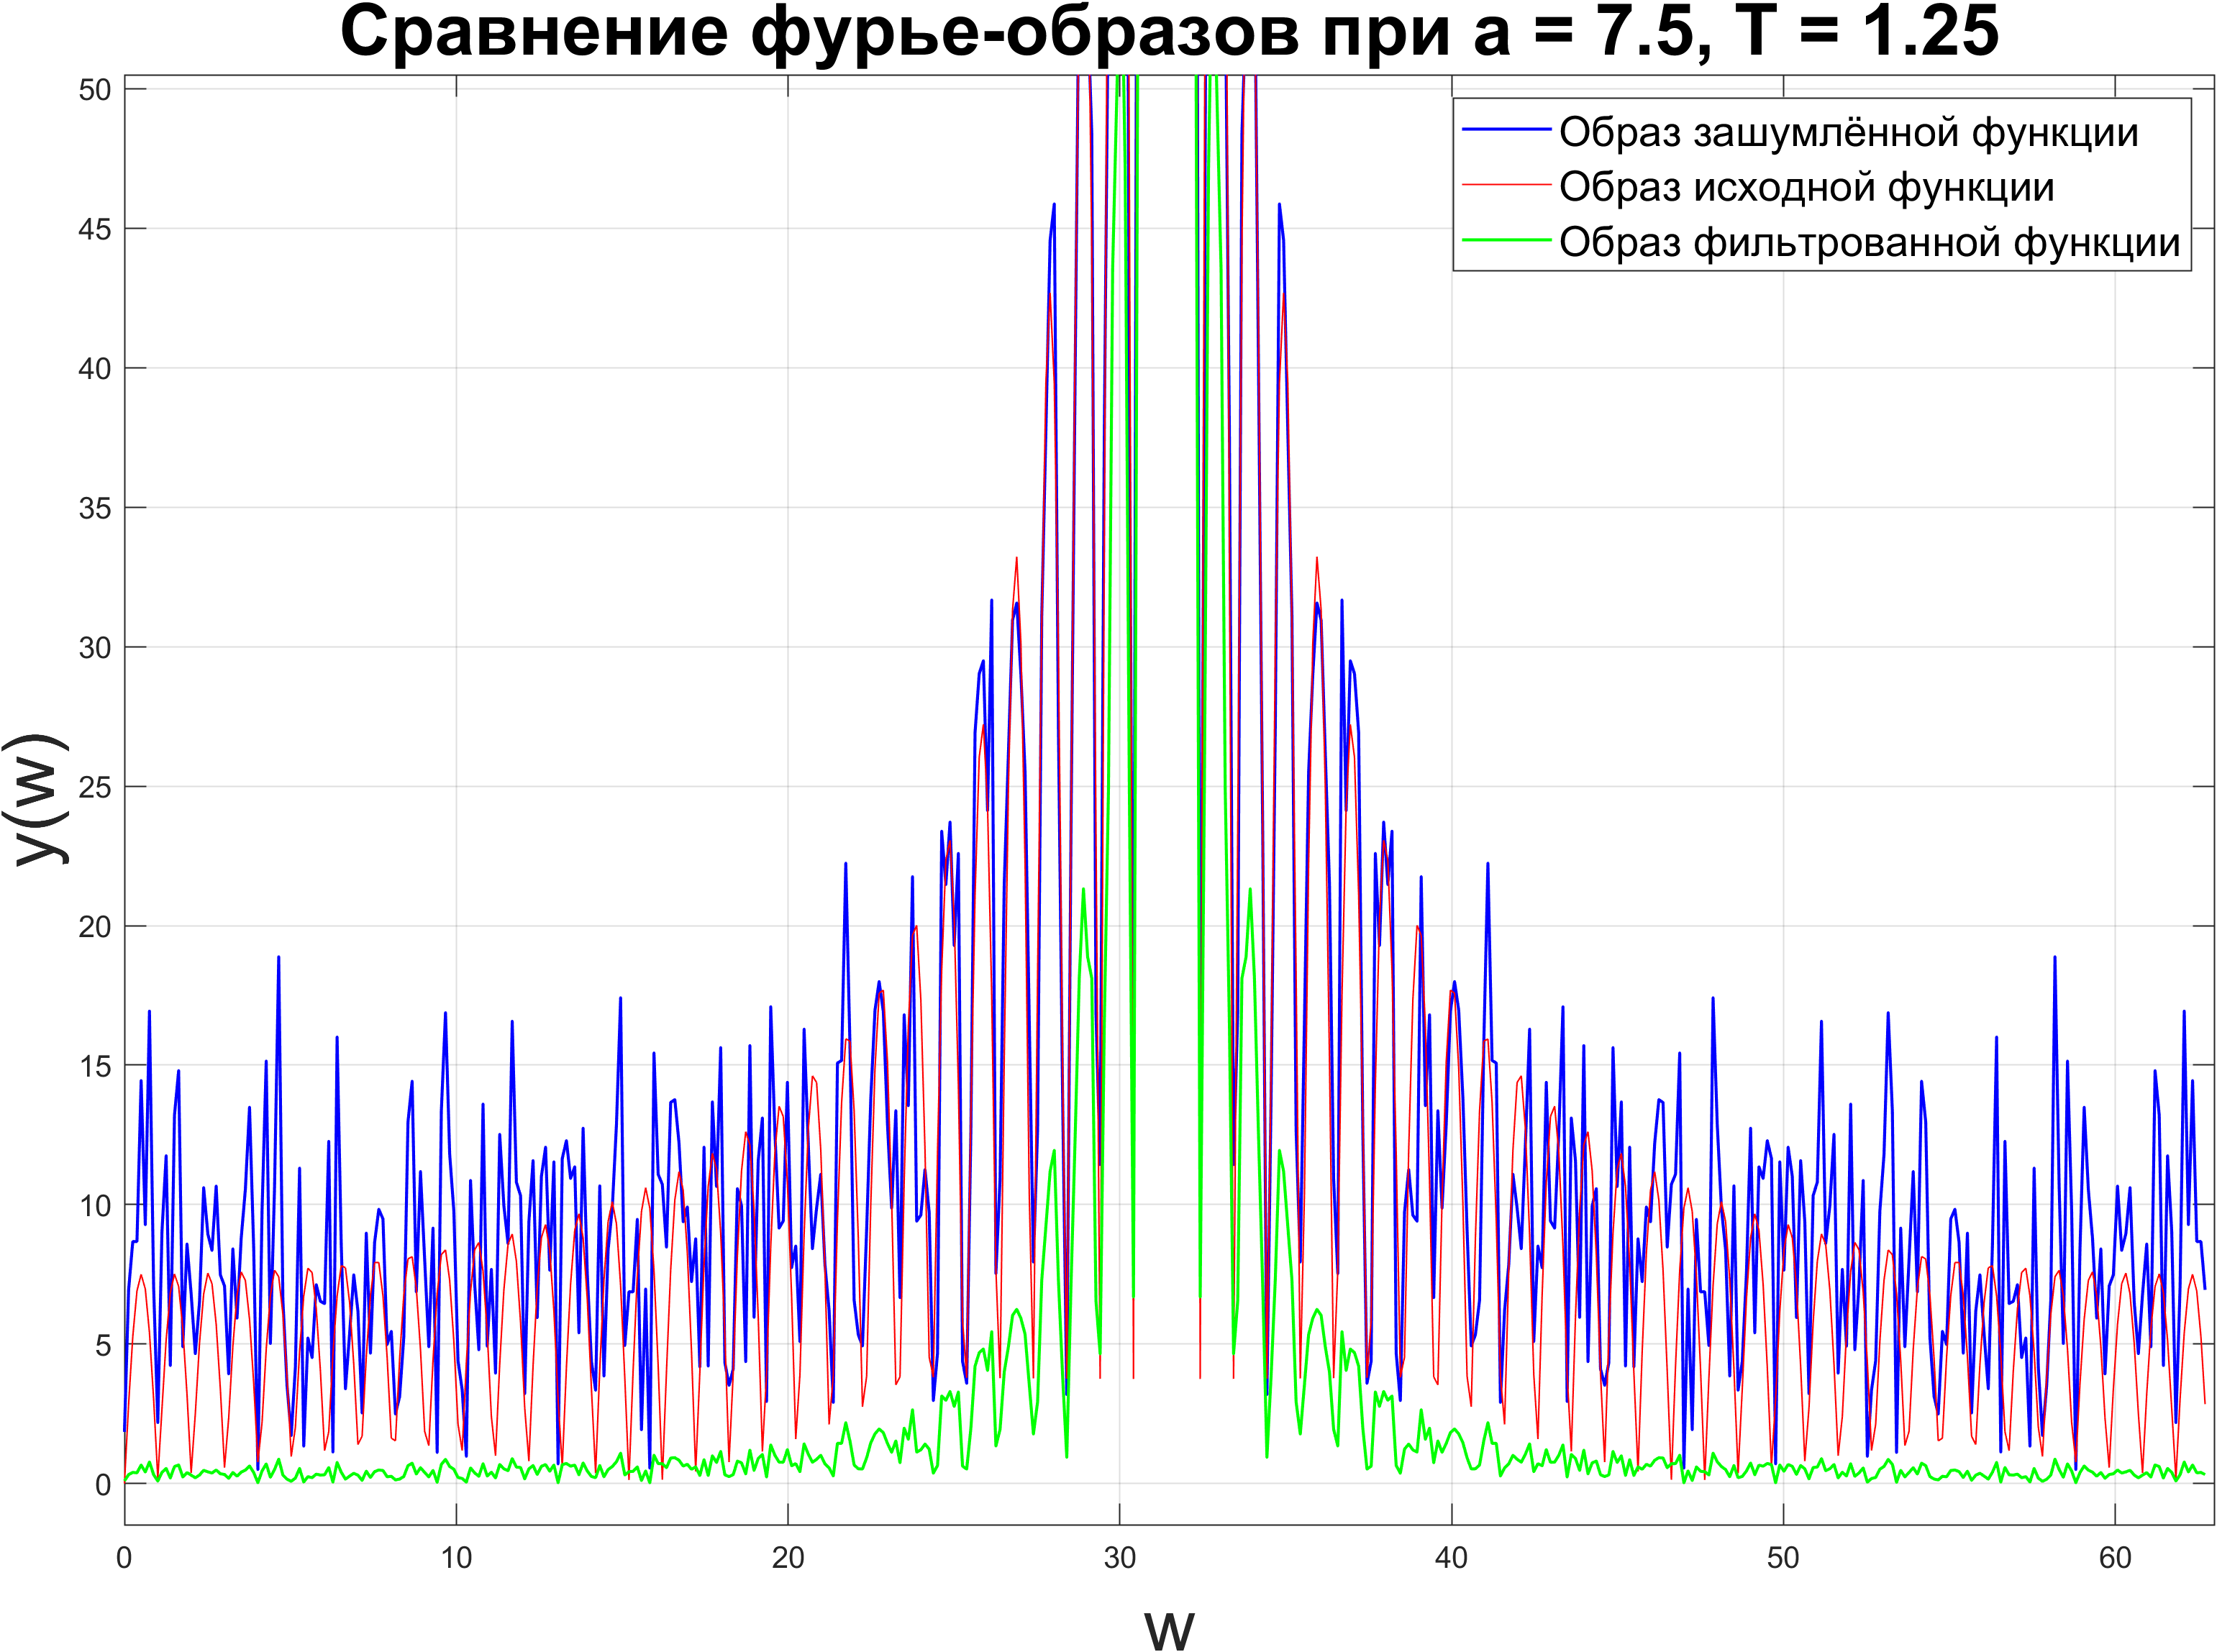
\includegraphics[width=0.90\textwidth, keepaspectratio]{images/fur_imgs_g_a_7.5.png}
    \caption{Фурье-образы при $a = 7.5$}
\end{figure}
\begin{figure}[H]
    \centering
    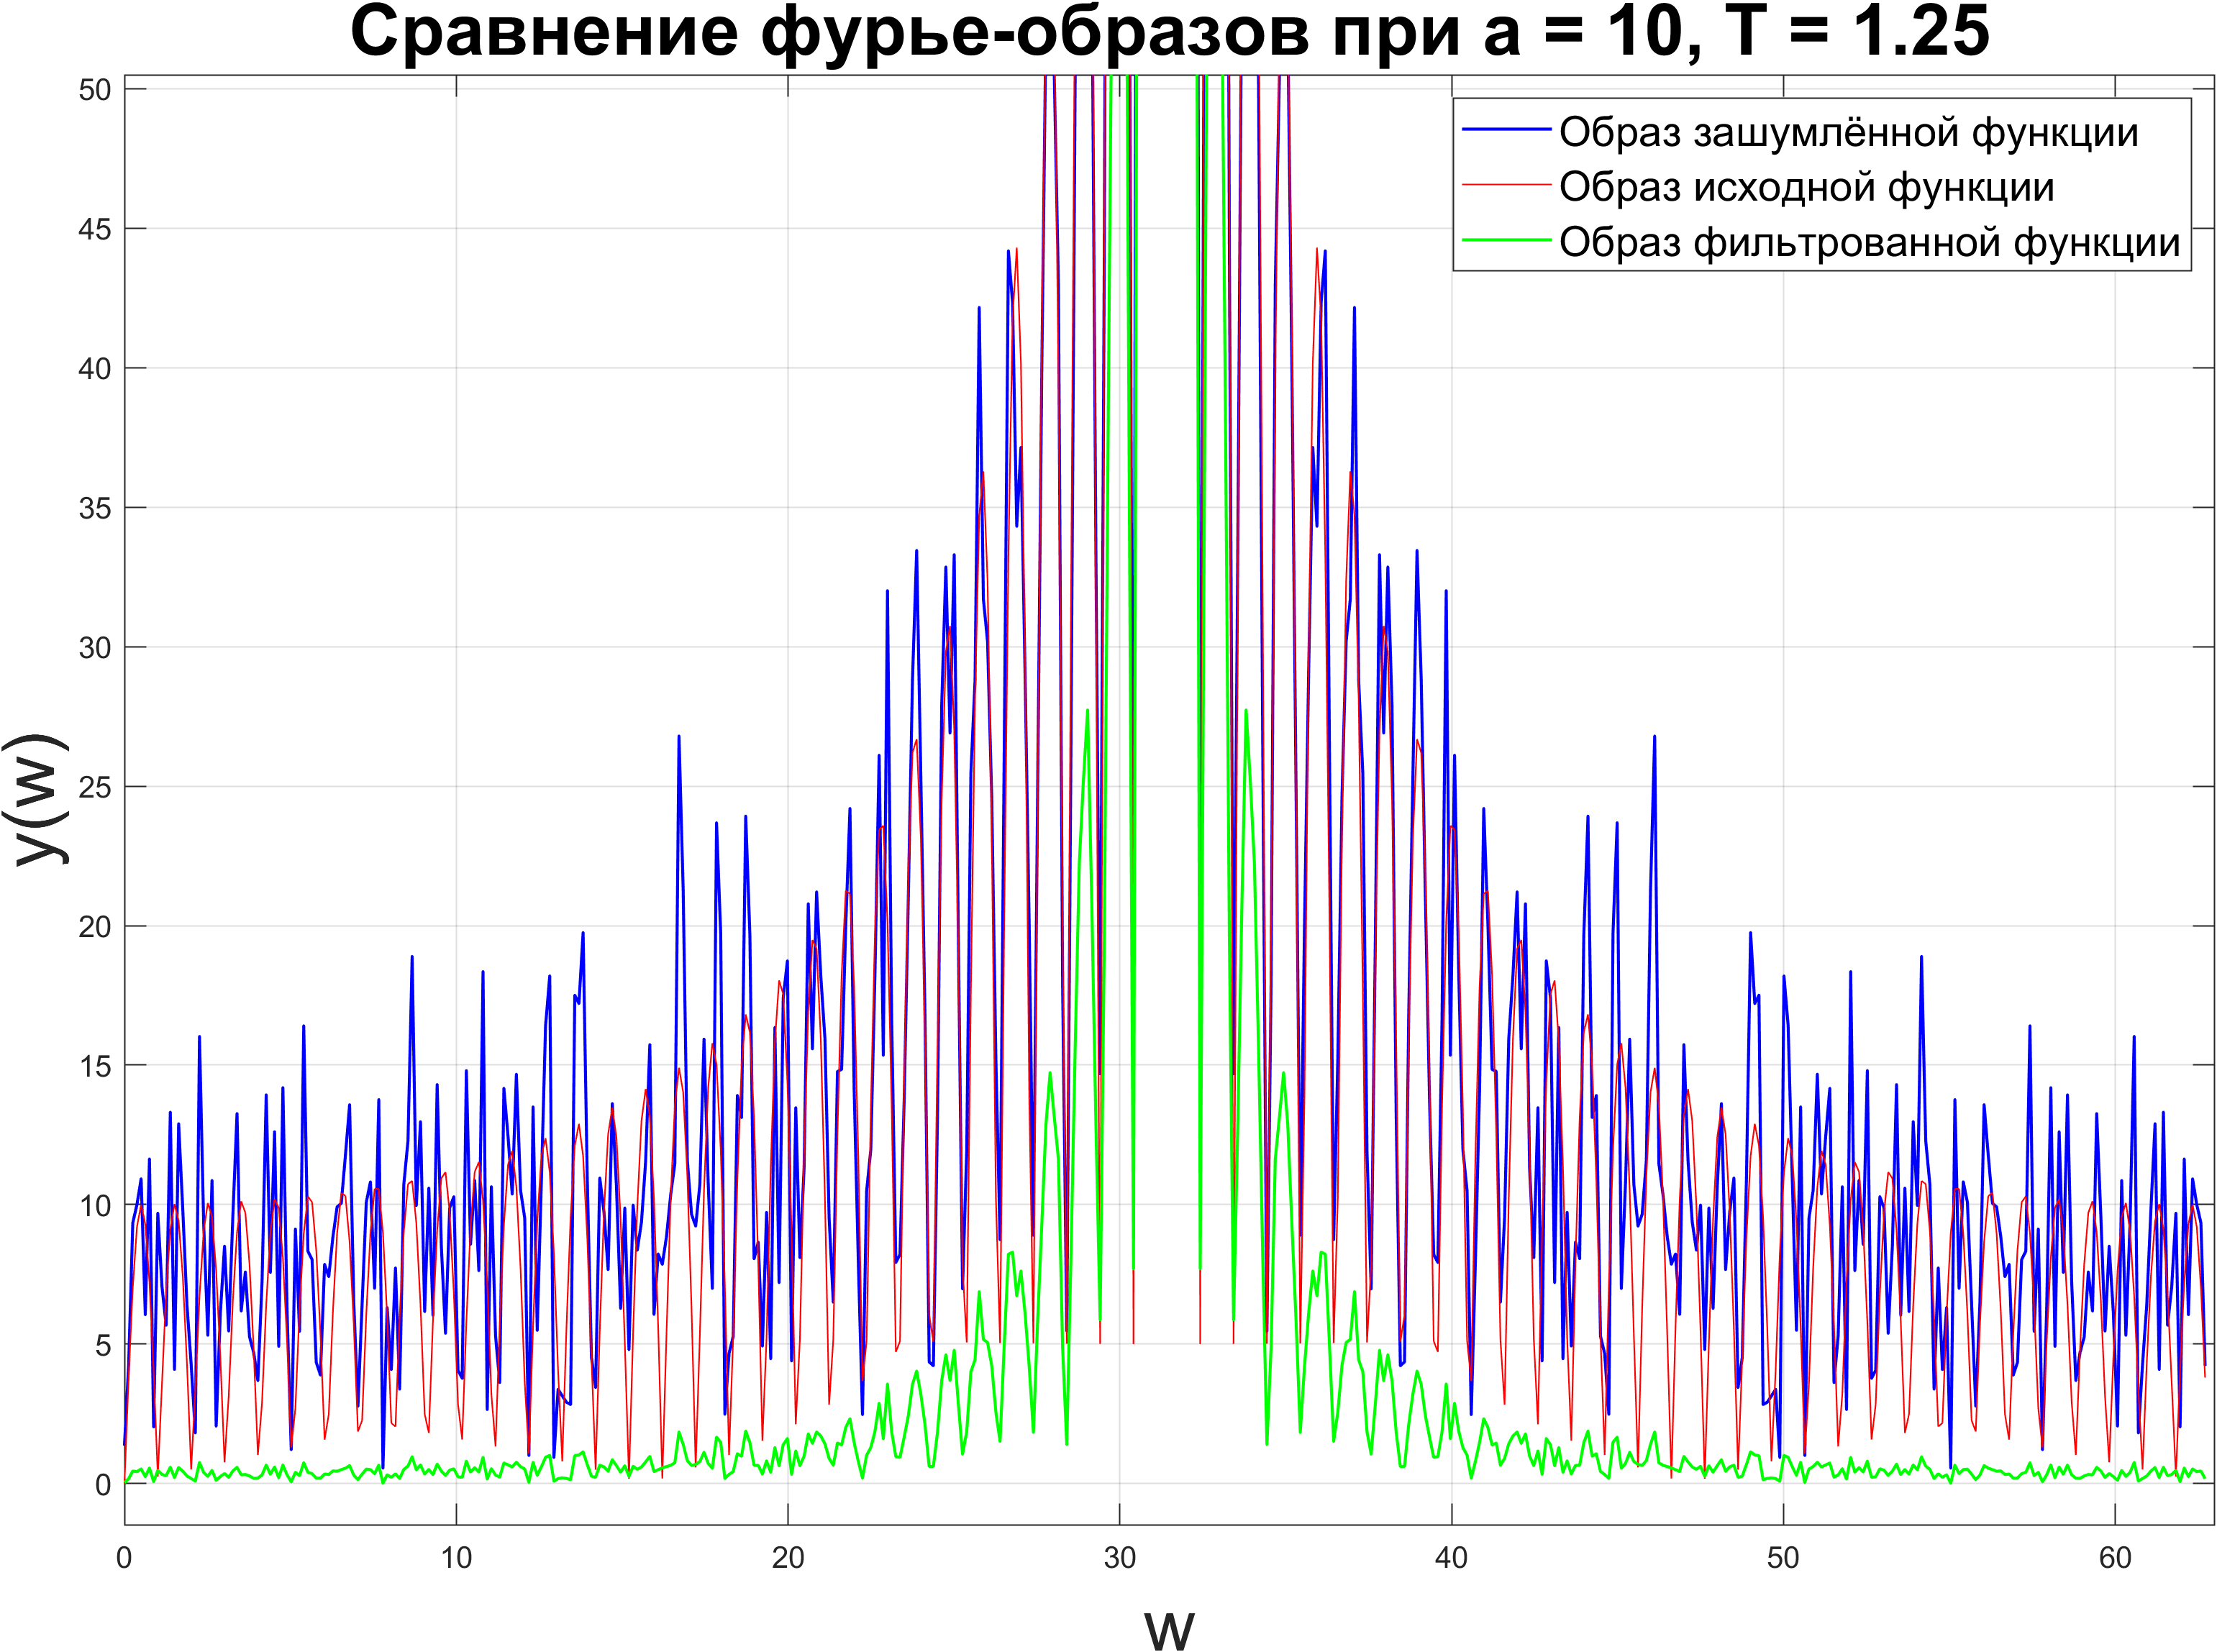
\includegraphics[width=0.90\textwidth, keepaspectratio]{images/fur_imgs_g_a_10.png}
    \caption{Фурье-образы при $a = 10.0$}
\end{figure}
\newpage
% ==========================================
% БЛОК 10: Фурье-образы (через передаточную функцию) при разных a
% ==========================================
\subsection{Фурье-образы $Y$, $y_{fil}$ (параметр $a$)}

\begin{figure}[H]
    \centering
    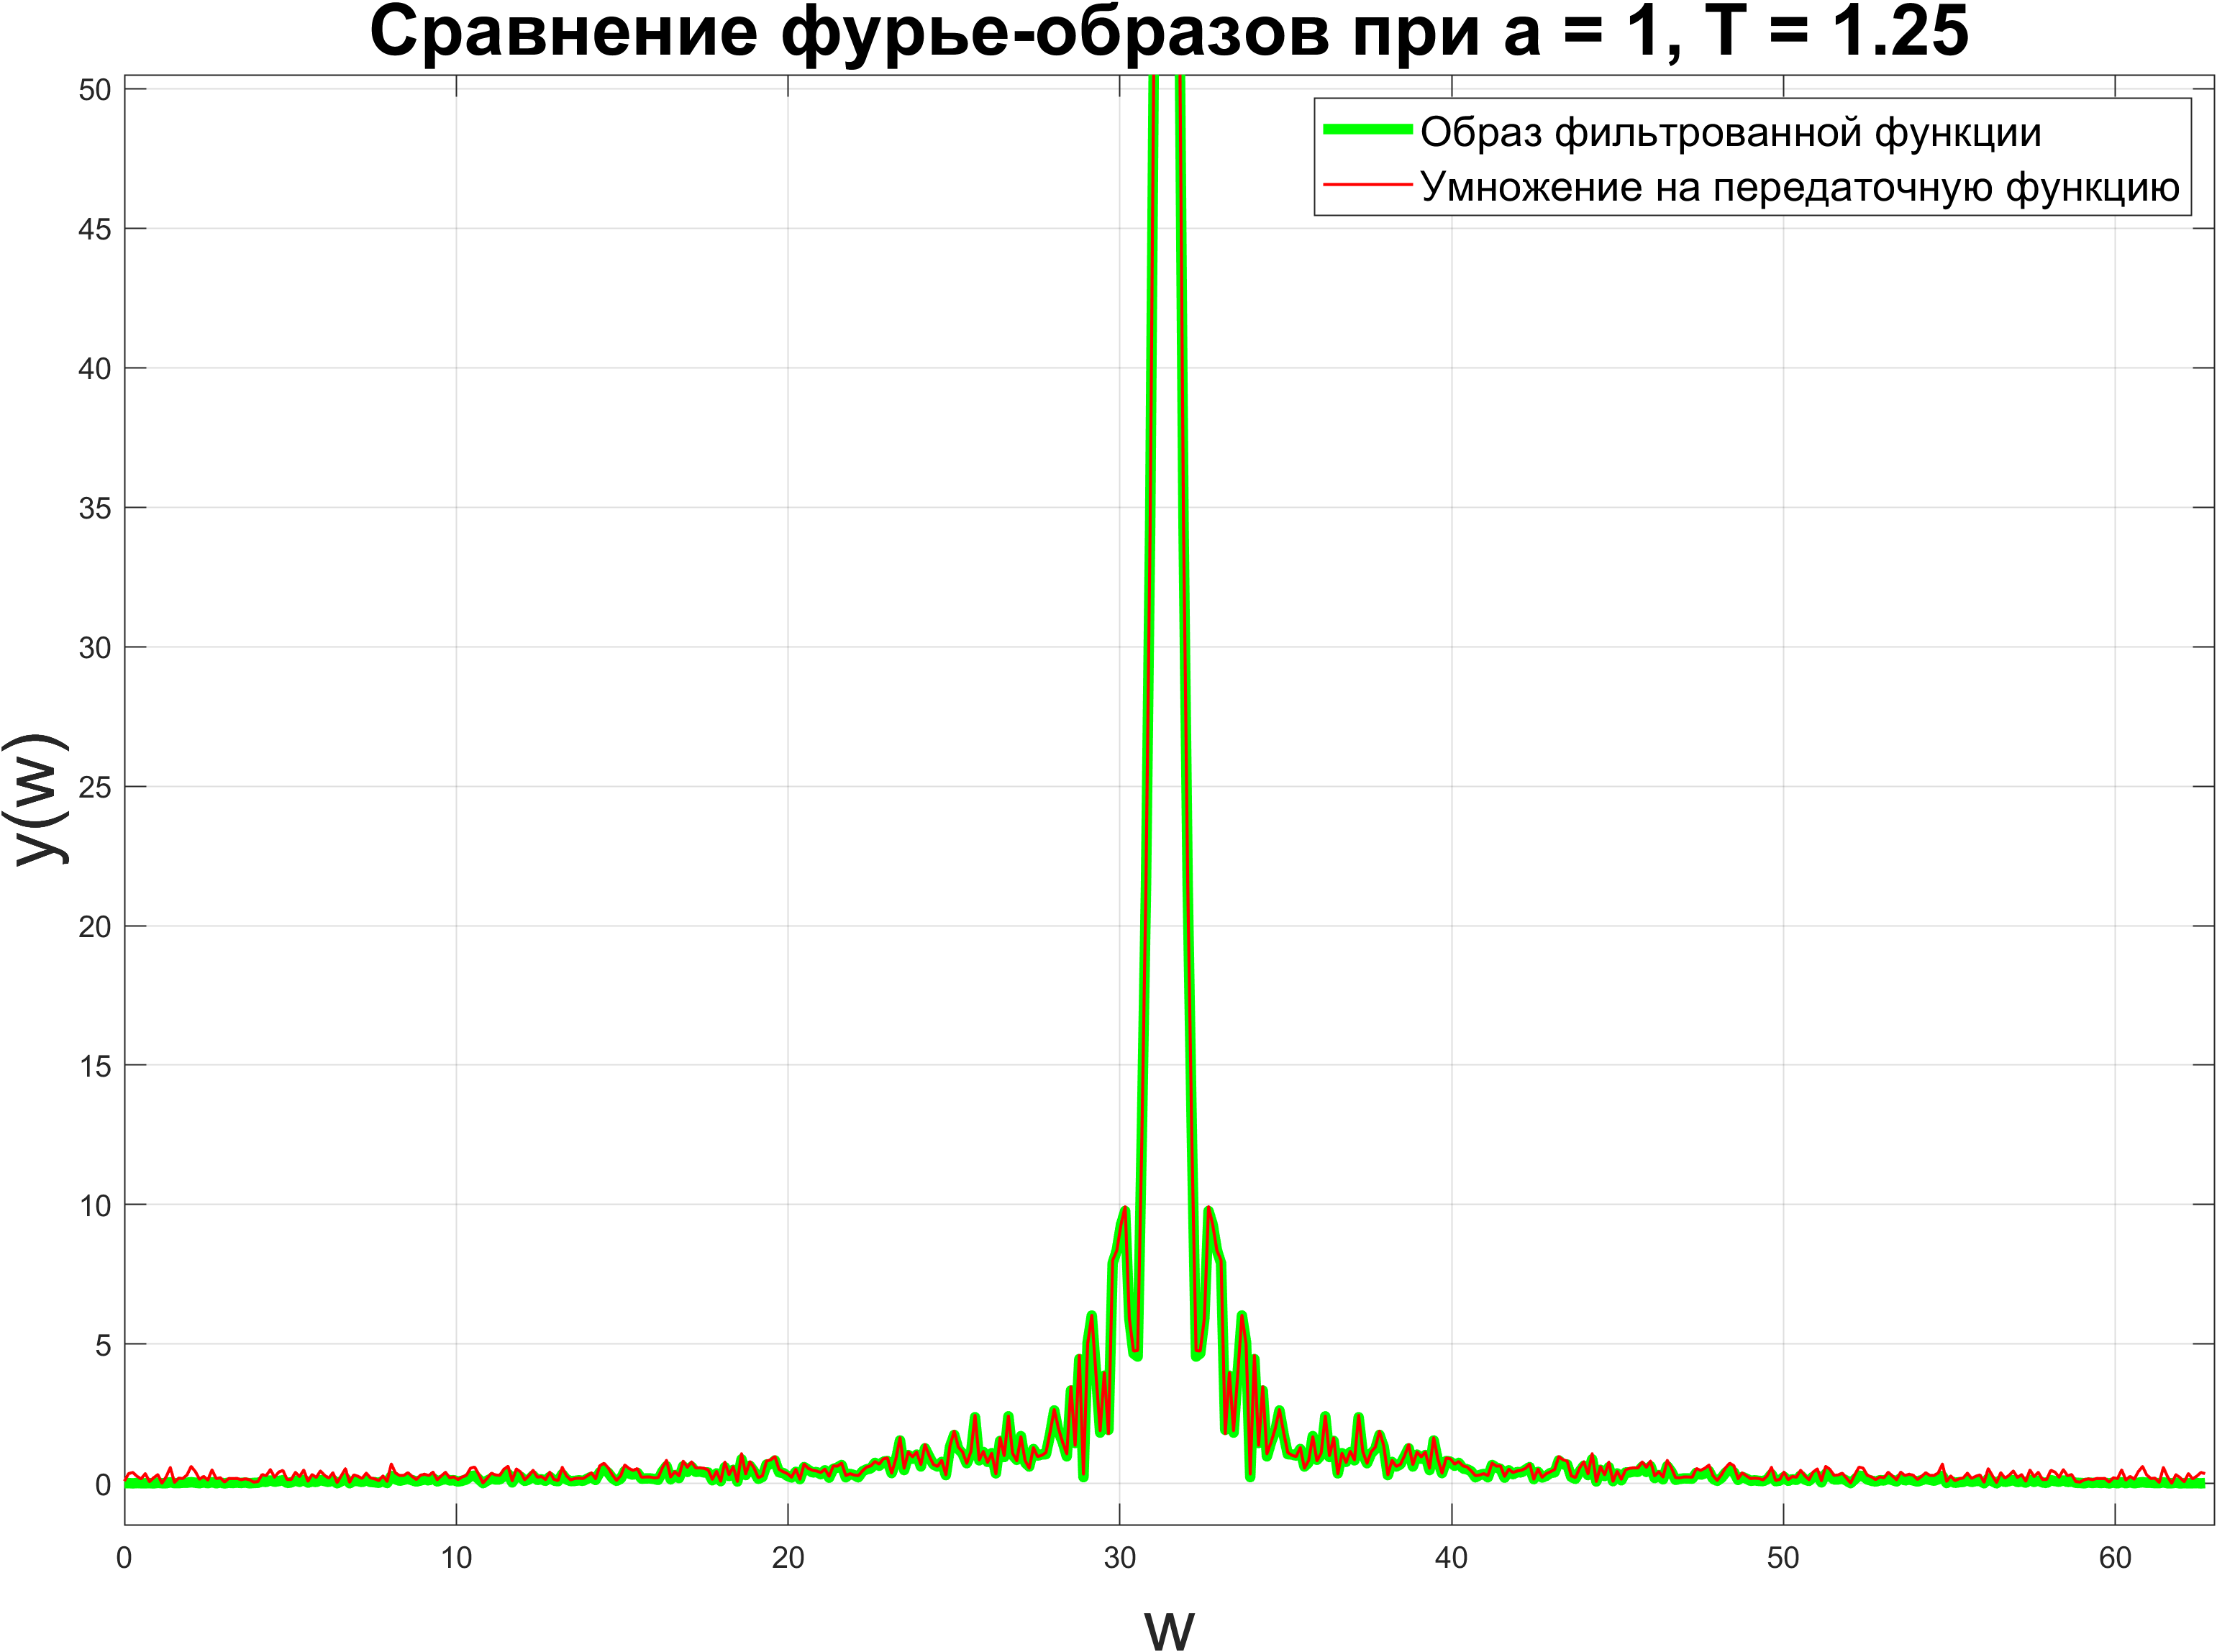
\includegraphics[width=0.85\textwidth, keepaspectratio]{images/fur_imgs_w_a_1.png}
    \caption{Фурье-образы через $H(\omega)$ при $a = 1.0$}
\end{figure}
\begin{figure}[H]
    \centering
    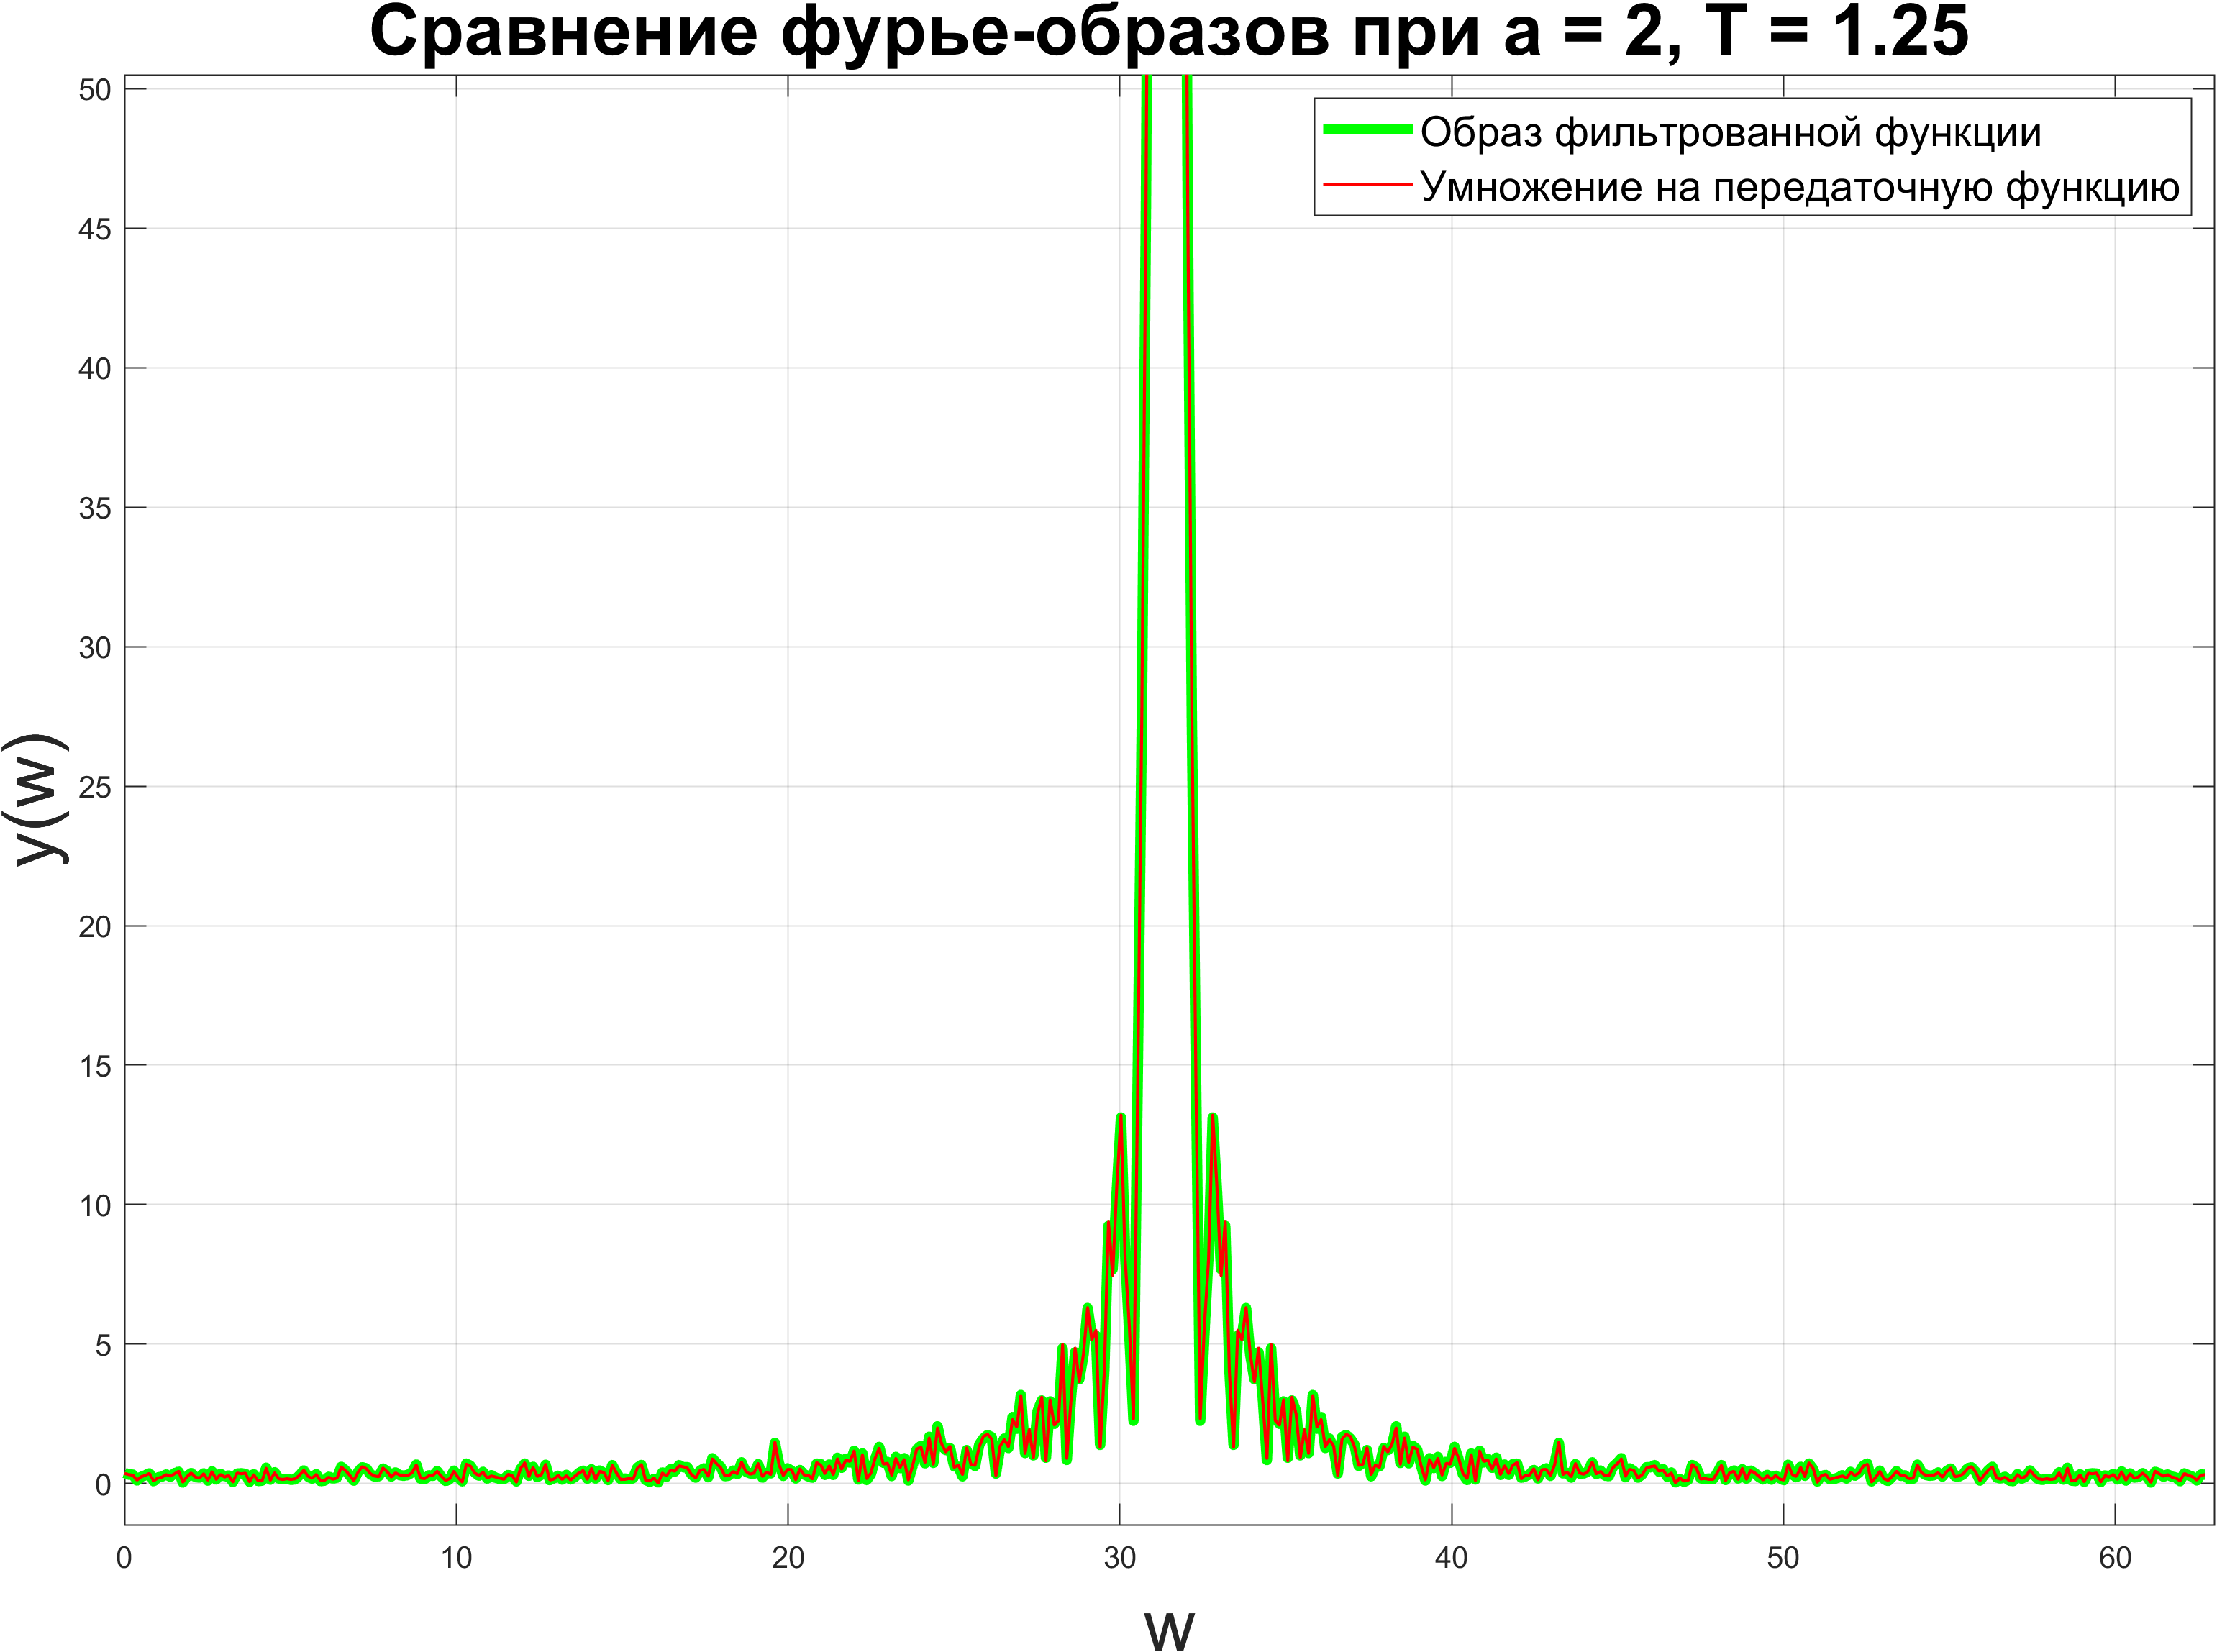
\includegraphics[width=0.85\textwidth, keepaspectratio]{images/fur_imgs_w_a_2.png}
    \caption{Фурье-образы через $H(\omega)$ при $a = 2.0$}
\end{figure}
\newpage

\begin{figure}[H]
    \centering
    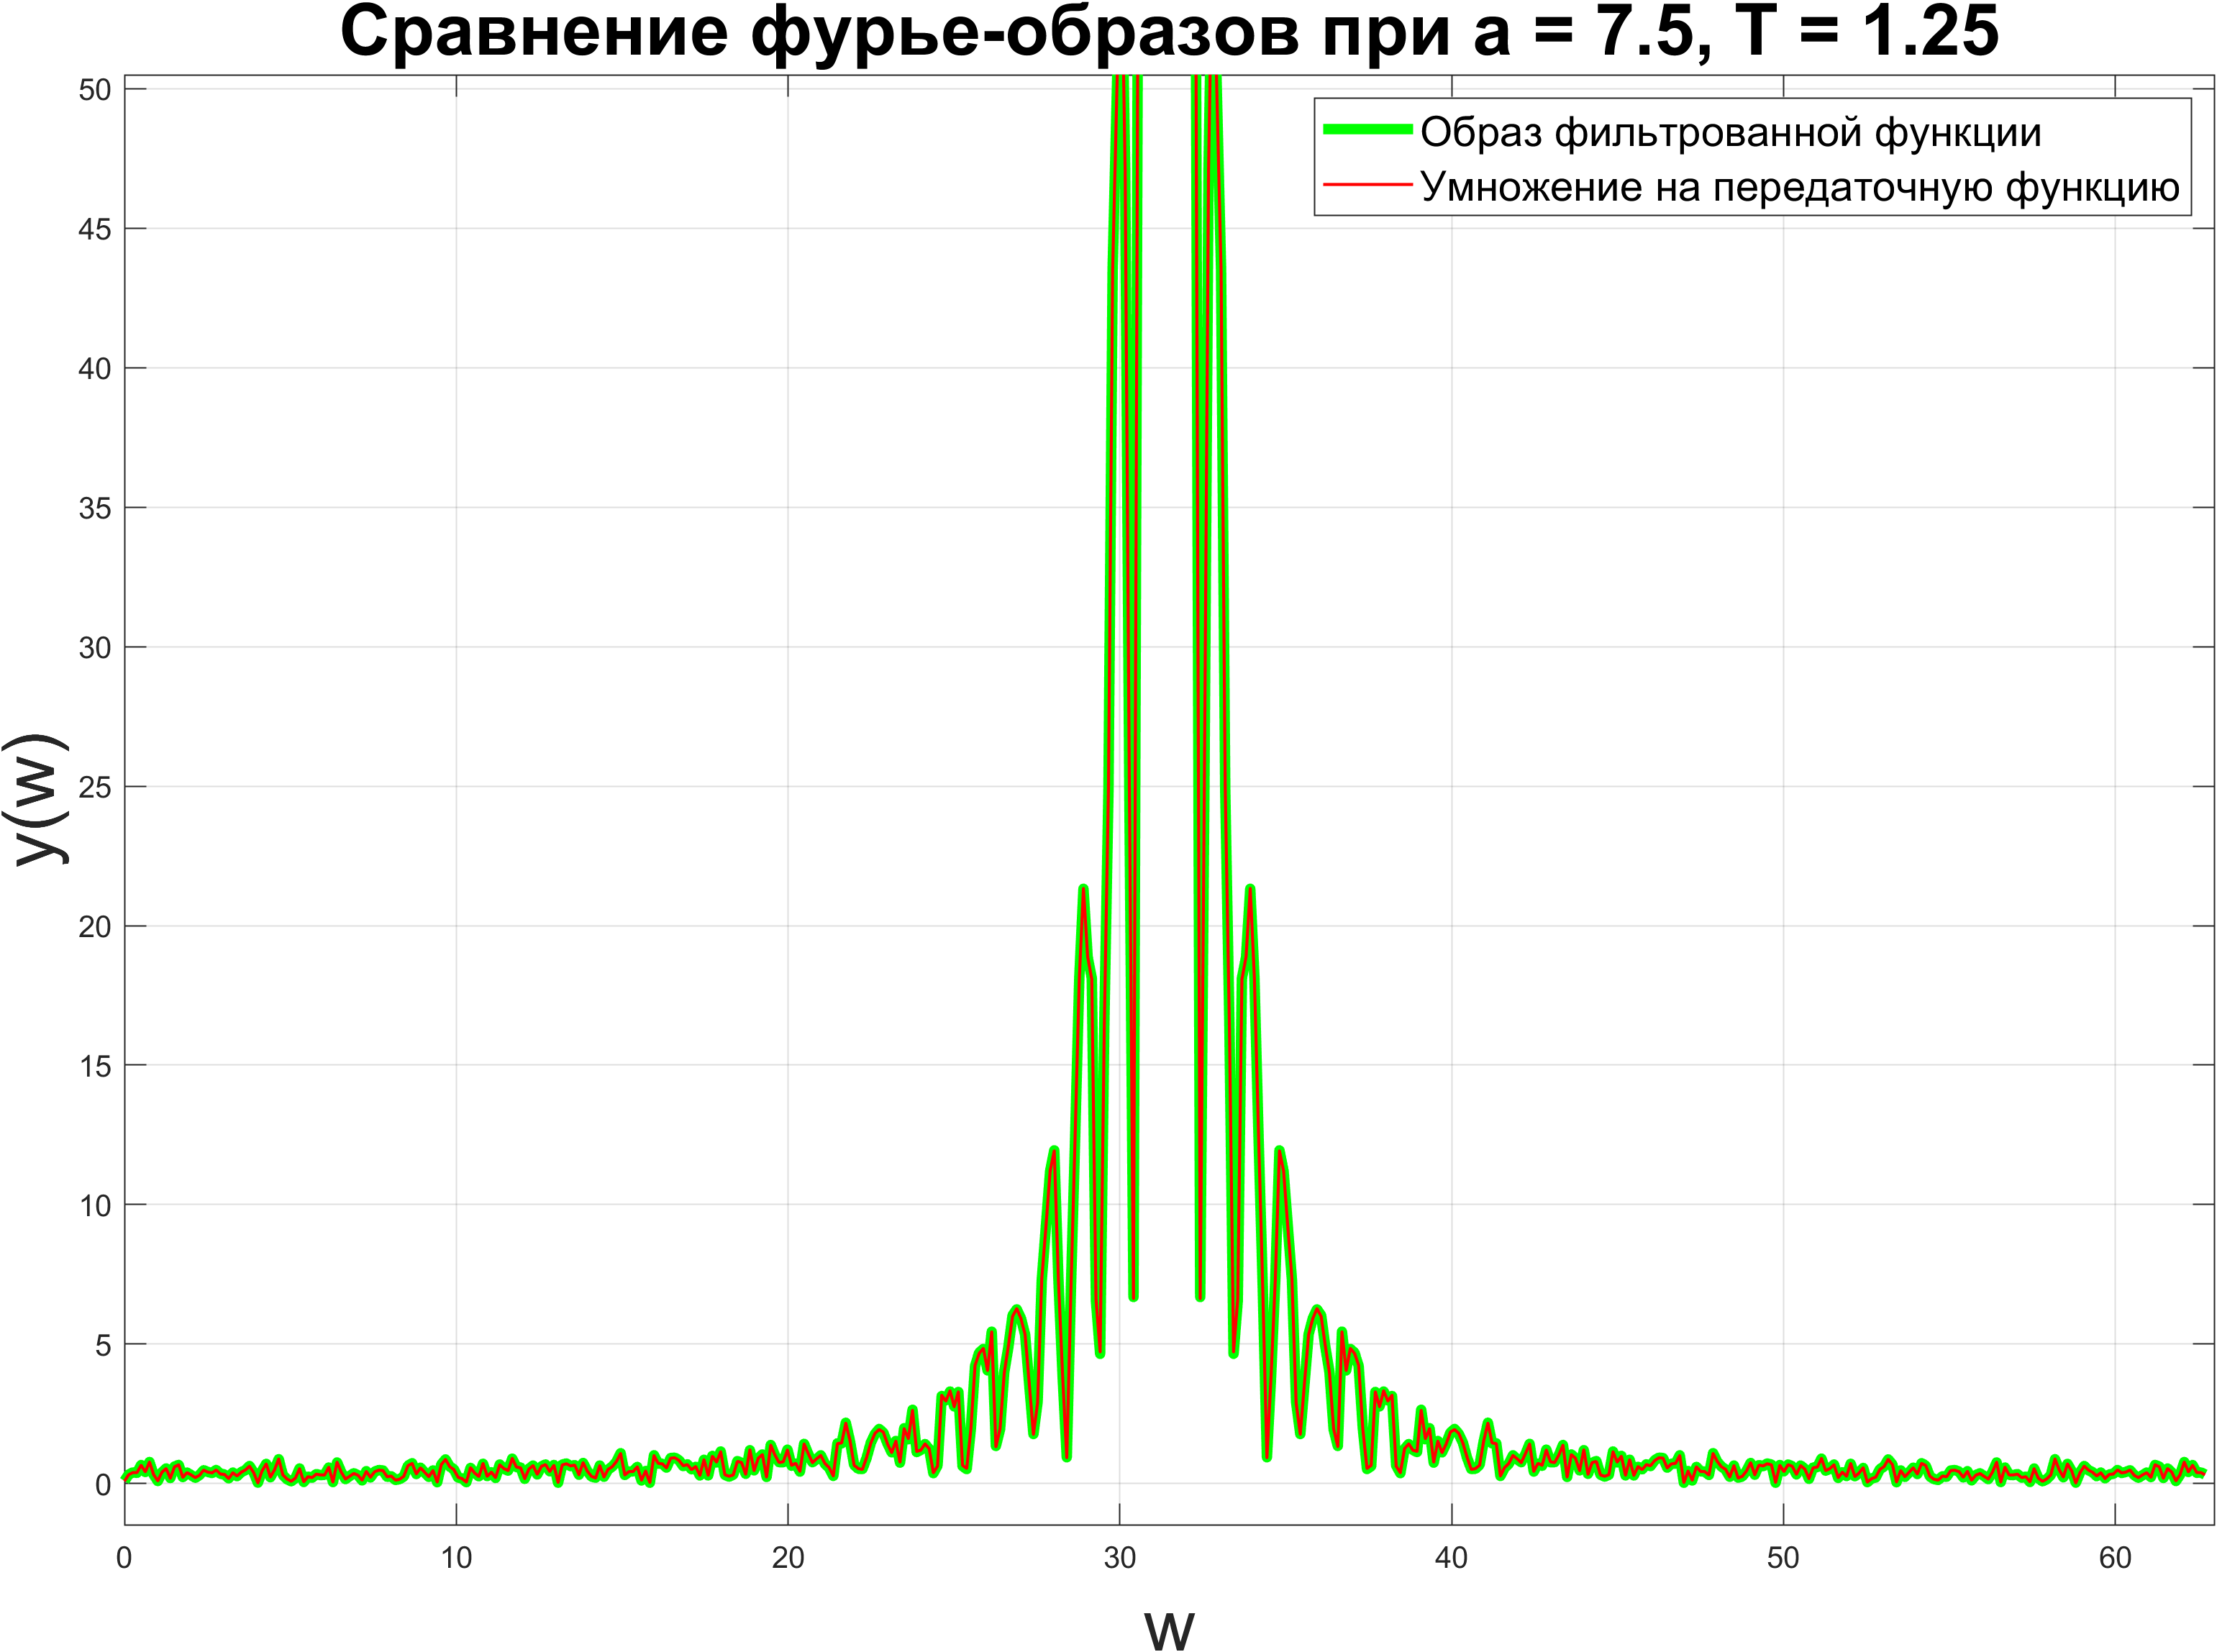
\includegraphics[width=0.90\textwidth, keepaspectratio]{images/fur_imgs_w_a_7.5.png}
    \caption{Фурье-образы через $H(\omega)$ при $a = 7.5$}
\end{figure}
\begin{figure}[H]
    \centering
    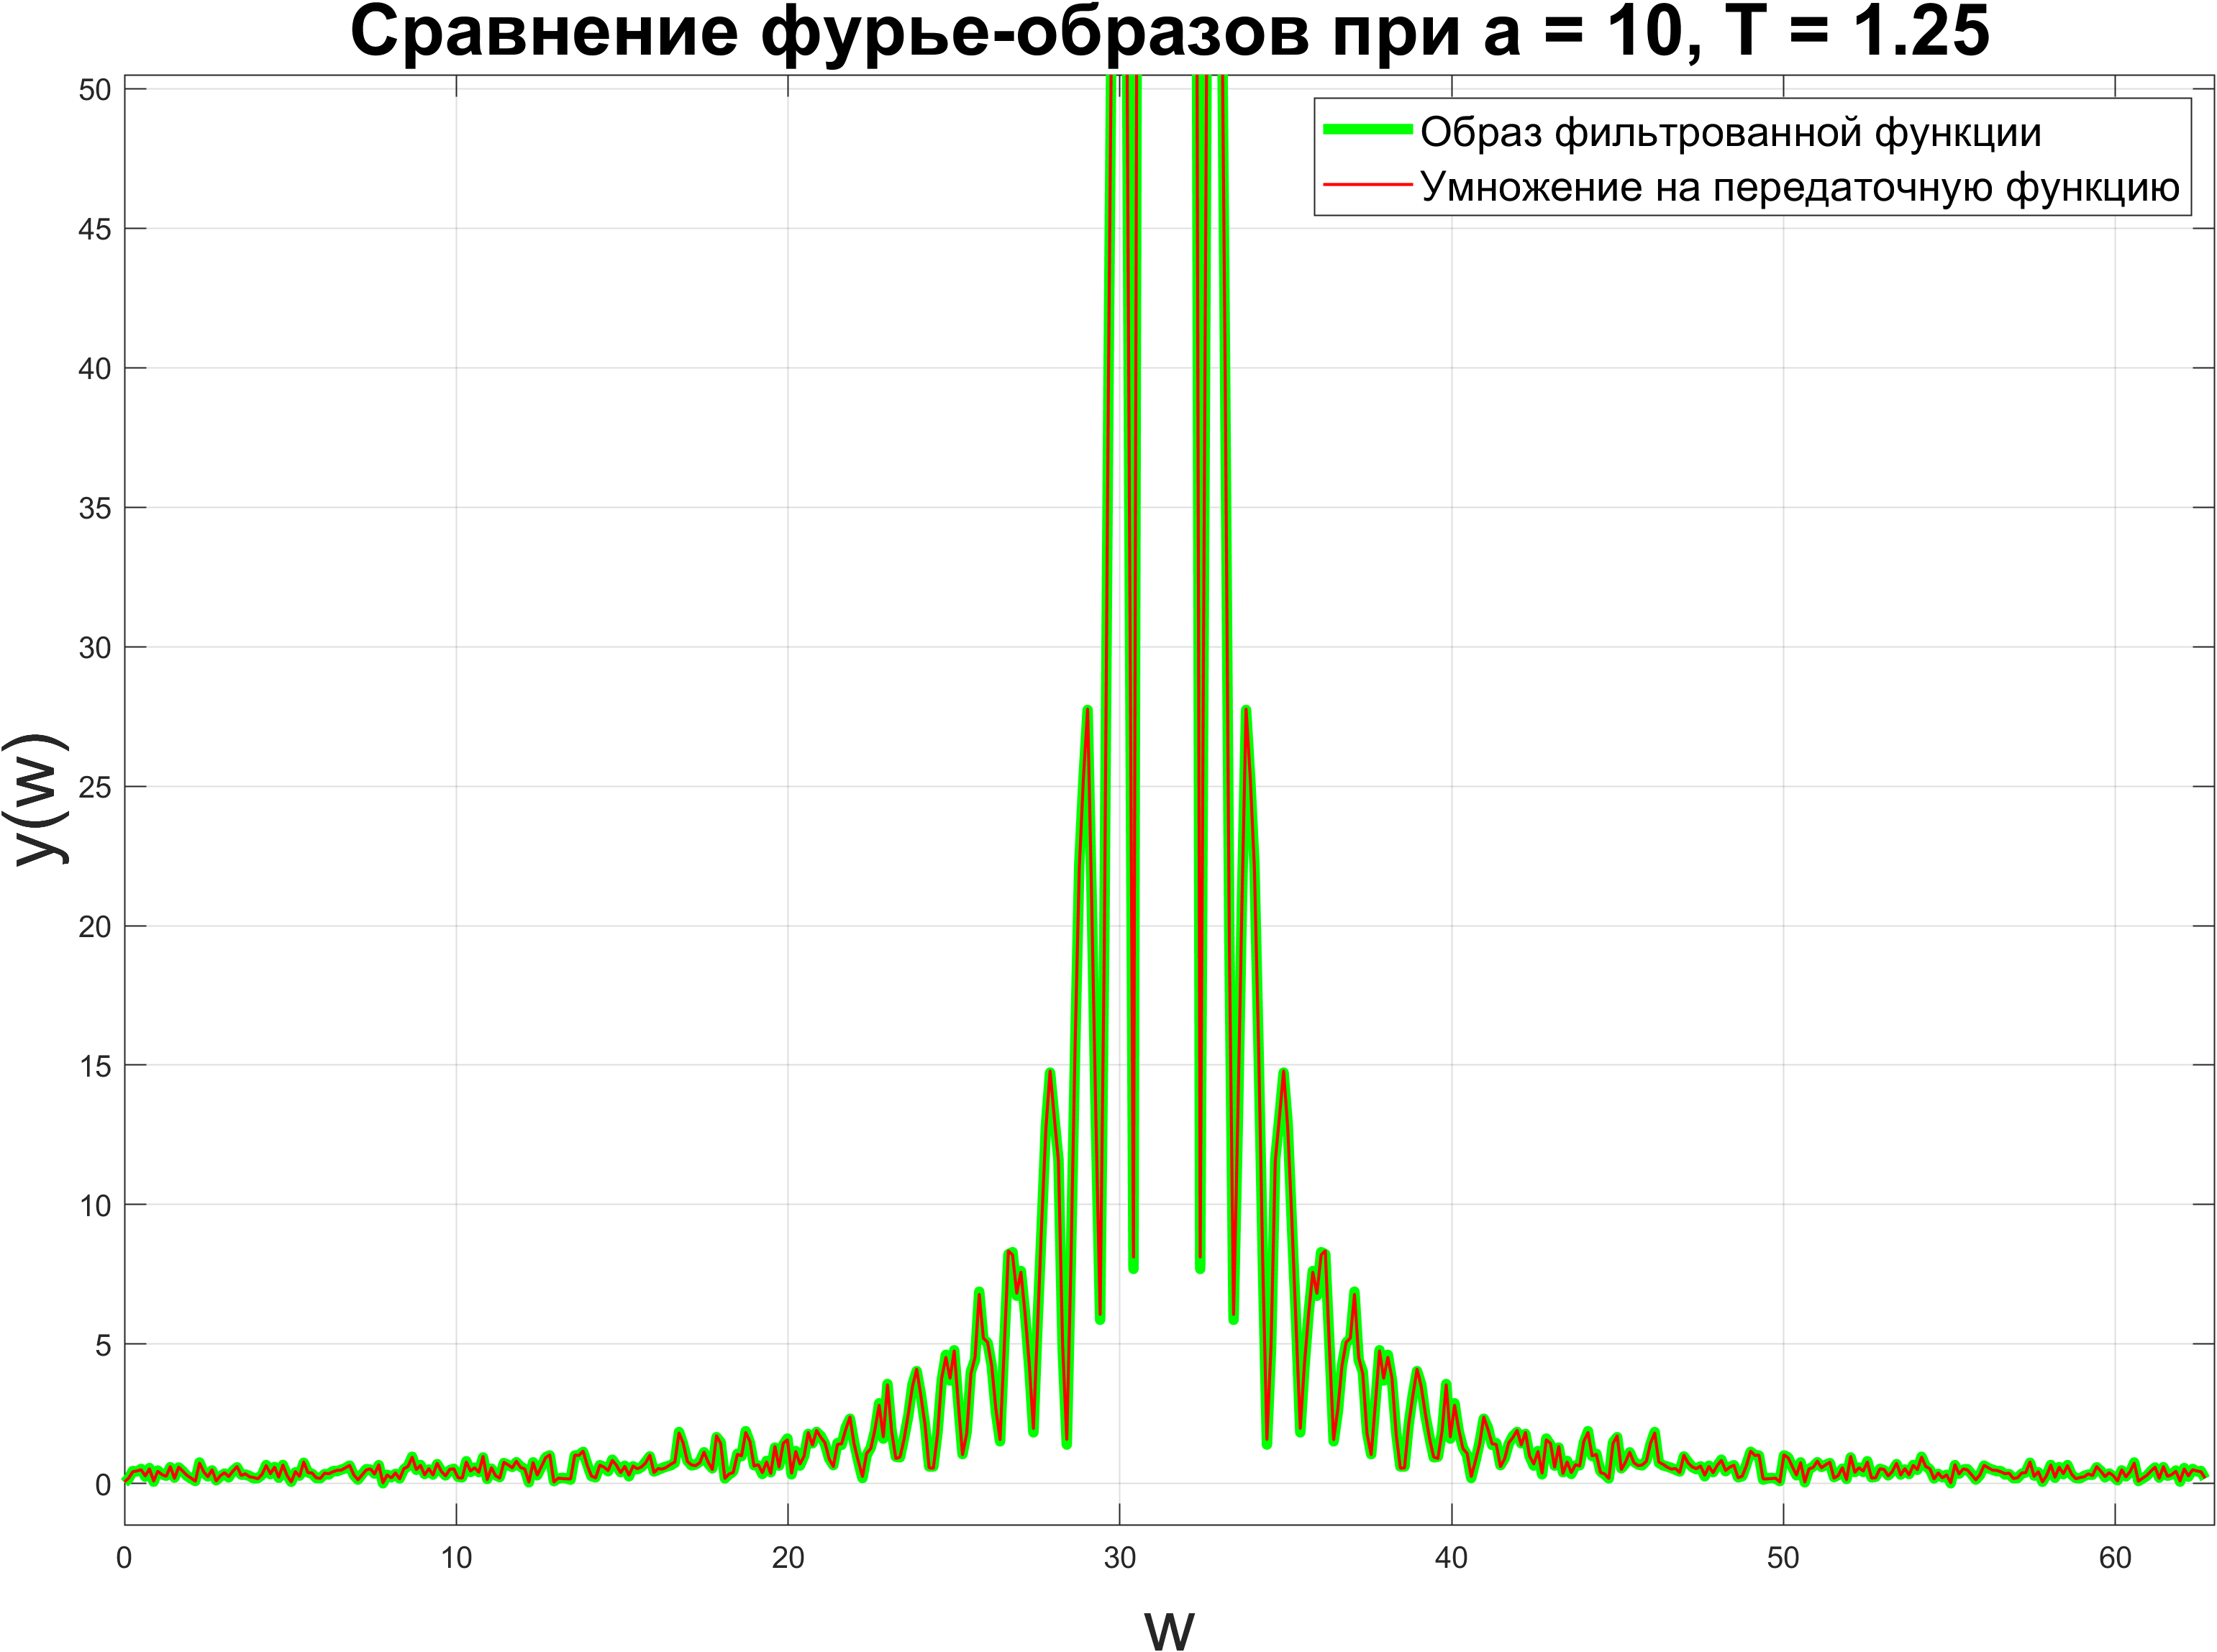
\includegraphics[width=0.90\textwidth, keepaspectratio]{images/fur_imgs_w_a_10.png}
    \caption{Фурье-образы через $H(\omega)$ при $a = 10.0$}
\end{figure}
\newpage

\subsection{Вывод}
Таким образом, видно, что фильтр помогает получить примерный исходный сигнал, но до определённой степени зашумлённости, при попытке
дальнейшего приближения сигнал искажается, поэтому фильтр довольно неточен. Скорее всего может использоваться для того,
чтобы сильно зашумлённый сигнал первично отфильтровать перед применением каких-нибудь других фильтров.
%\begin{figure}[H]
%    \centering
%    
\includegraphics[width=1.0\linewidth]{images/filtered_muha.png}
%    \caption{Исходный и отфильтрованный сигналы}
%    \label{fig:noise}
%\end{figure}
\newpage
\section{Режекторный полосовой фильтр}
\subsection{Описание фильтра}
Теперь зашумим функцию $g(t)$ шумом постоянной частоты:
\[
u(t) = g(t) + 0,5sin(d \cdot t)
\]
Рассмотрим динамический фильтр вида:
\[
W(p) = \frac{p^2 + a_1 p + a_2}{p^2 + b_1 p + b_2},
\]
такой что:
\newline
1) корни уравнения $p^2 + b_1 p + b_2$, $p_1, p_2$ имеют отрицательную вещественную часть;
\newline
2) при $\omega \rightarrow 0$ и при $\omega \rightarrow \infty$, $|W(i\omega)| \rightarrow 1$;
\newline
3) при $\omega = \omega_0$, $|W(i\omega)| = 0$.
\newline
По теореме Виета:
$p_1 \cdot p_2 = b_2, \ \ p_1 + p_2 = -b_1$
\newline
Отсюда $b_1 > 0, \ \ b_2 > 0$.
\[
|W(i \omega)| = |\frac{-\omega^2 + ia_1\omega + a_2}{-\omega^2 + ib_1\omega + b_2}|
\]
При $\omega = 0$:
\[
|W(i \omega)| = \frac{a_2}{b_2} = 1 => a_2 = b_2
\]
При $\omega \rightarrow \infty$:
\[
|W(i \omega)| = |\frac{\omega^2(-1 + \frac{ia_1}{\omega} + \frac{a_2}{\omega^2})}{\omega^2(-1 + \frac{ib_1}{\omega} + \frac{b_2}{\omega^2})}| \rightarrow 1, \textit{при любых} \ \ a_1, a_2, b_1, b_2
\]
При $\omega = \omega_0$:
\[
|W(i\omega_0)| = 0 <=> -\omega_0 ^ 2 + ia_1\omega_0 + a2 = 0
\]
Так как $\omega_0$ - действительное, получаем что $a_1 = 0$, $a_2 = \omega_0^2$. 
\newpage
\subsection{$d = \omega_0$}
Вначале рассмотрим $d = \omega_0 = \sqrt{a_2} = \sqrt{b_2} = 5$, и исследуем различные значения $b_1$:
\newline
Амплитудно-частотные характеристики:
\begin{figure}[H]
    \centering
    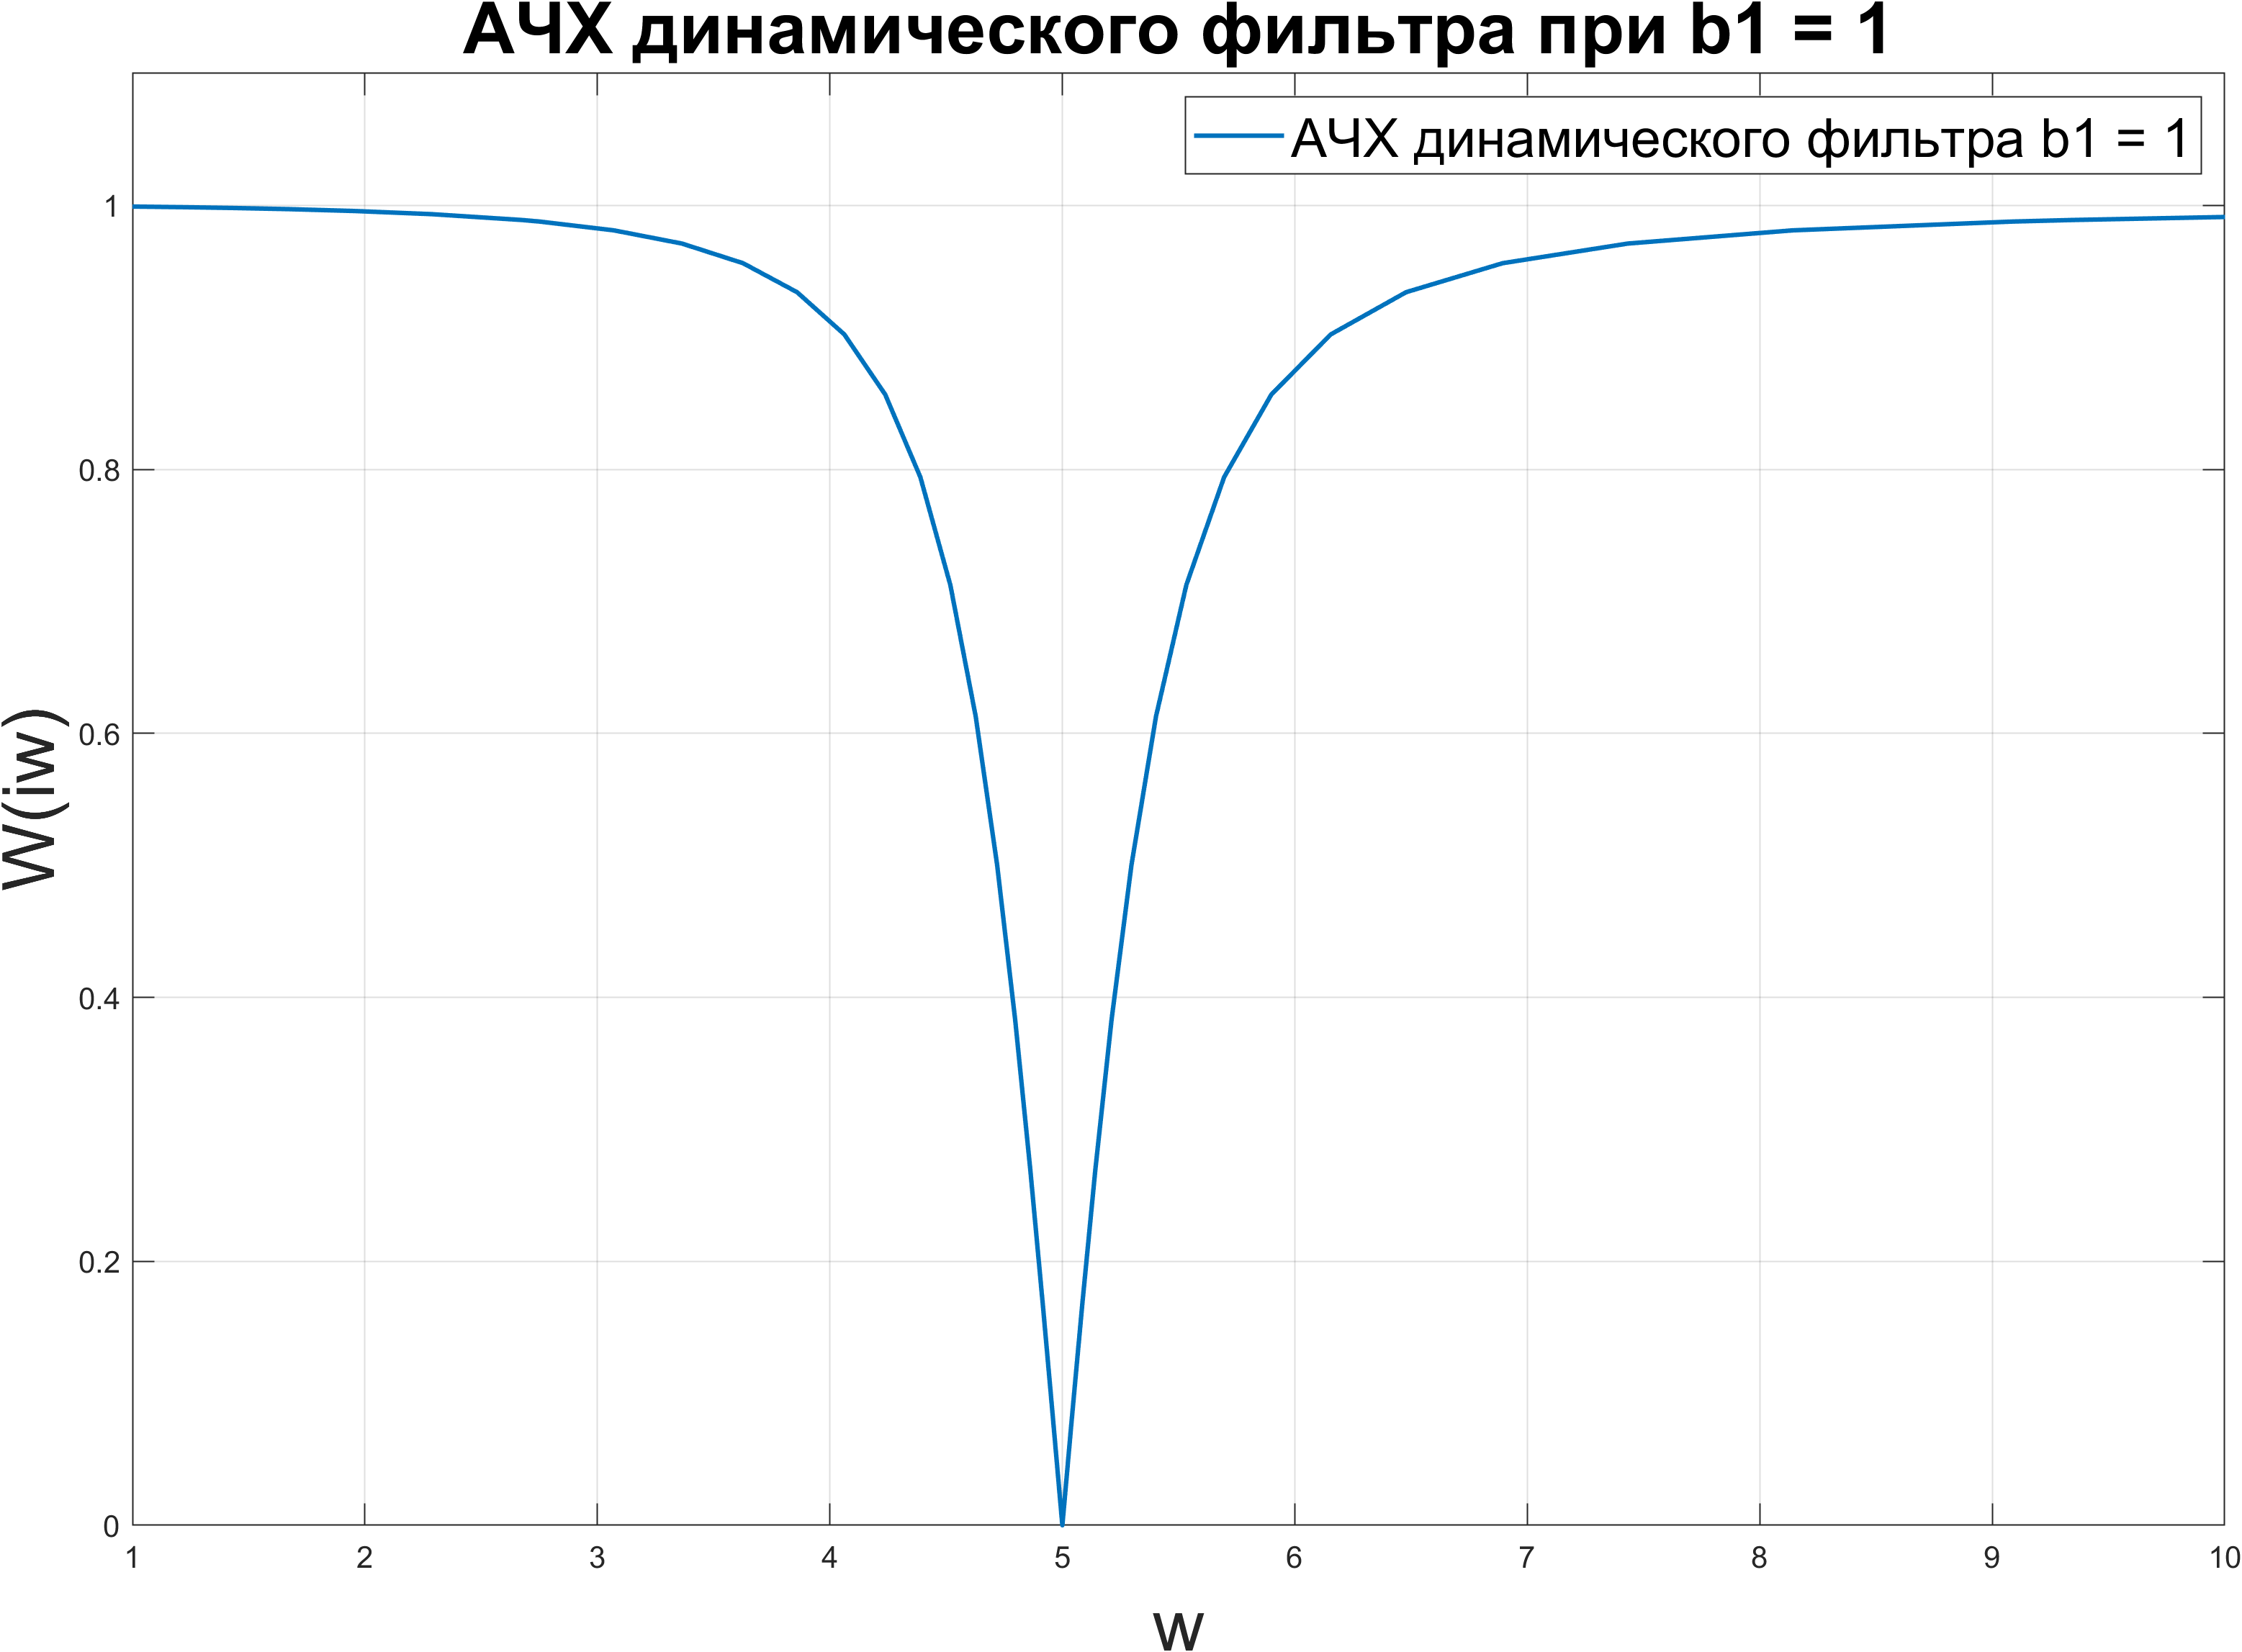
\includegraphics[width=0.83\textwidth, keepaspectratio]{images2/filter_ach_b1_1.png}
    \caption{АЧХ при $b_1 = 1$}
\end{figure}
\begin{figure}[H]
    \centering
    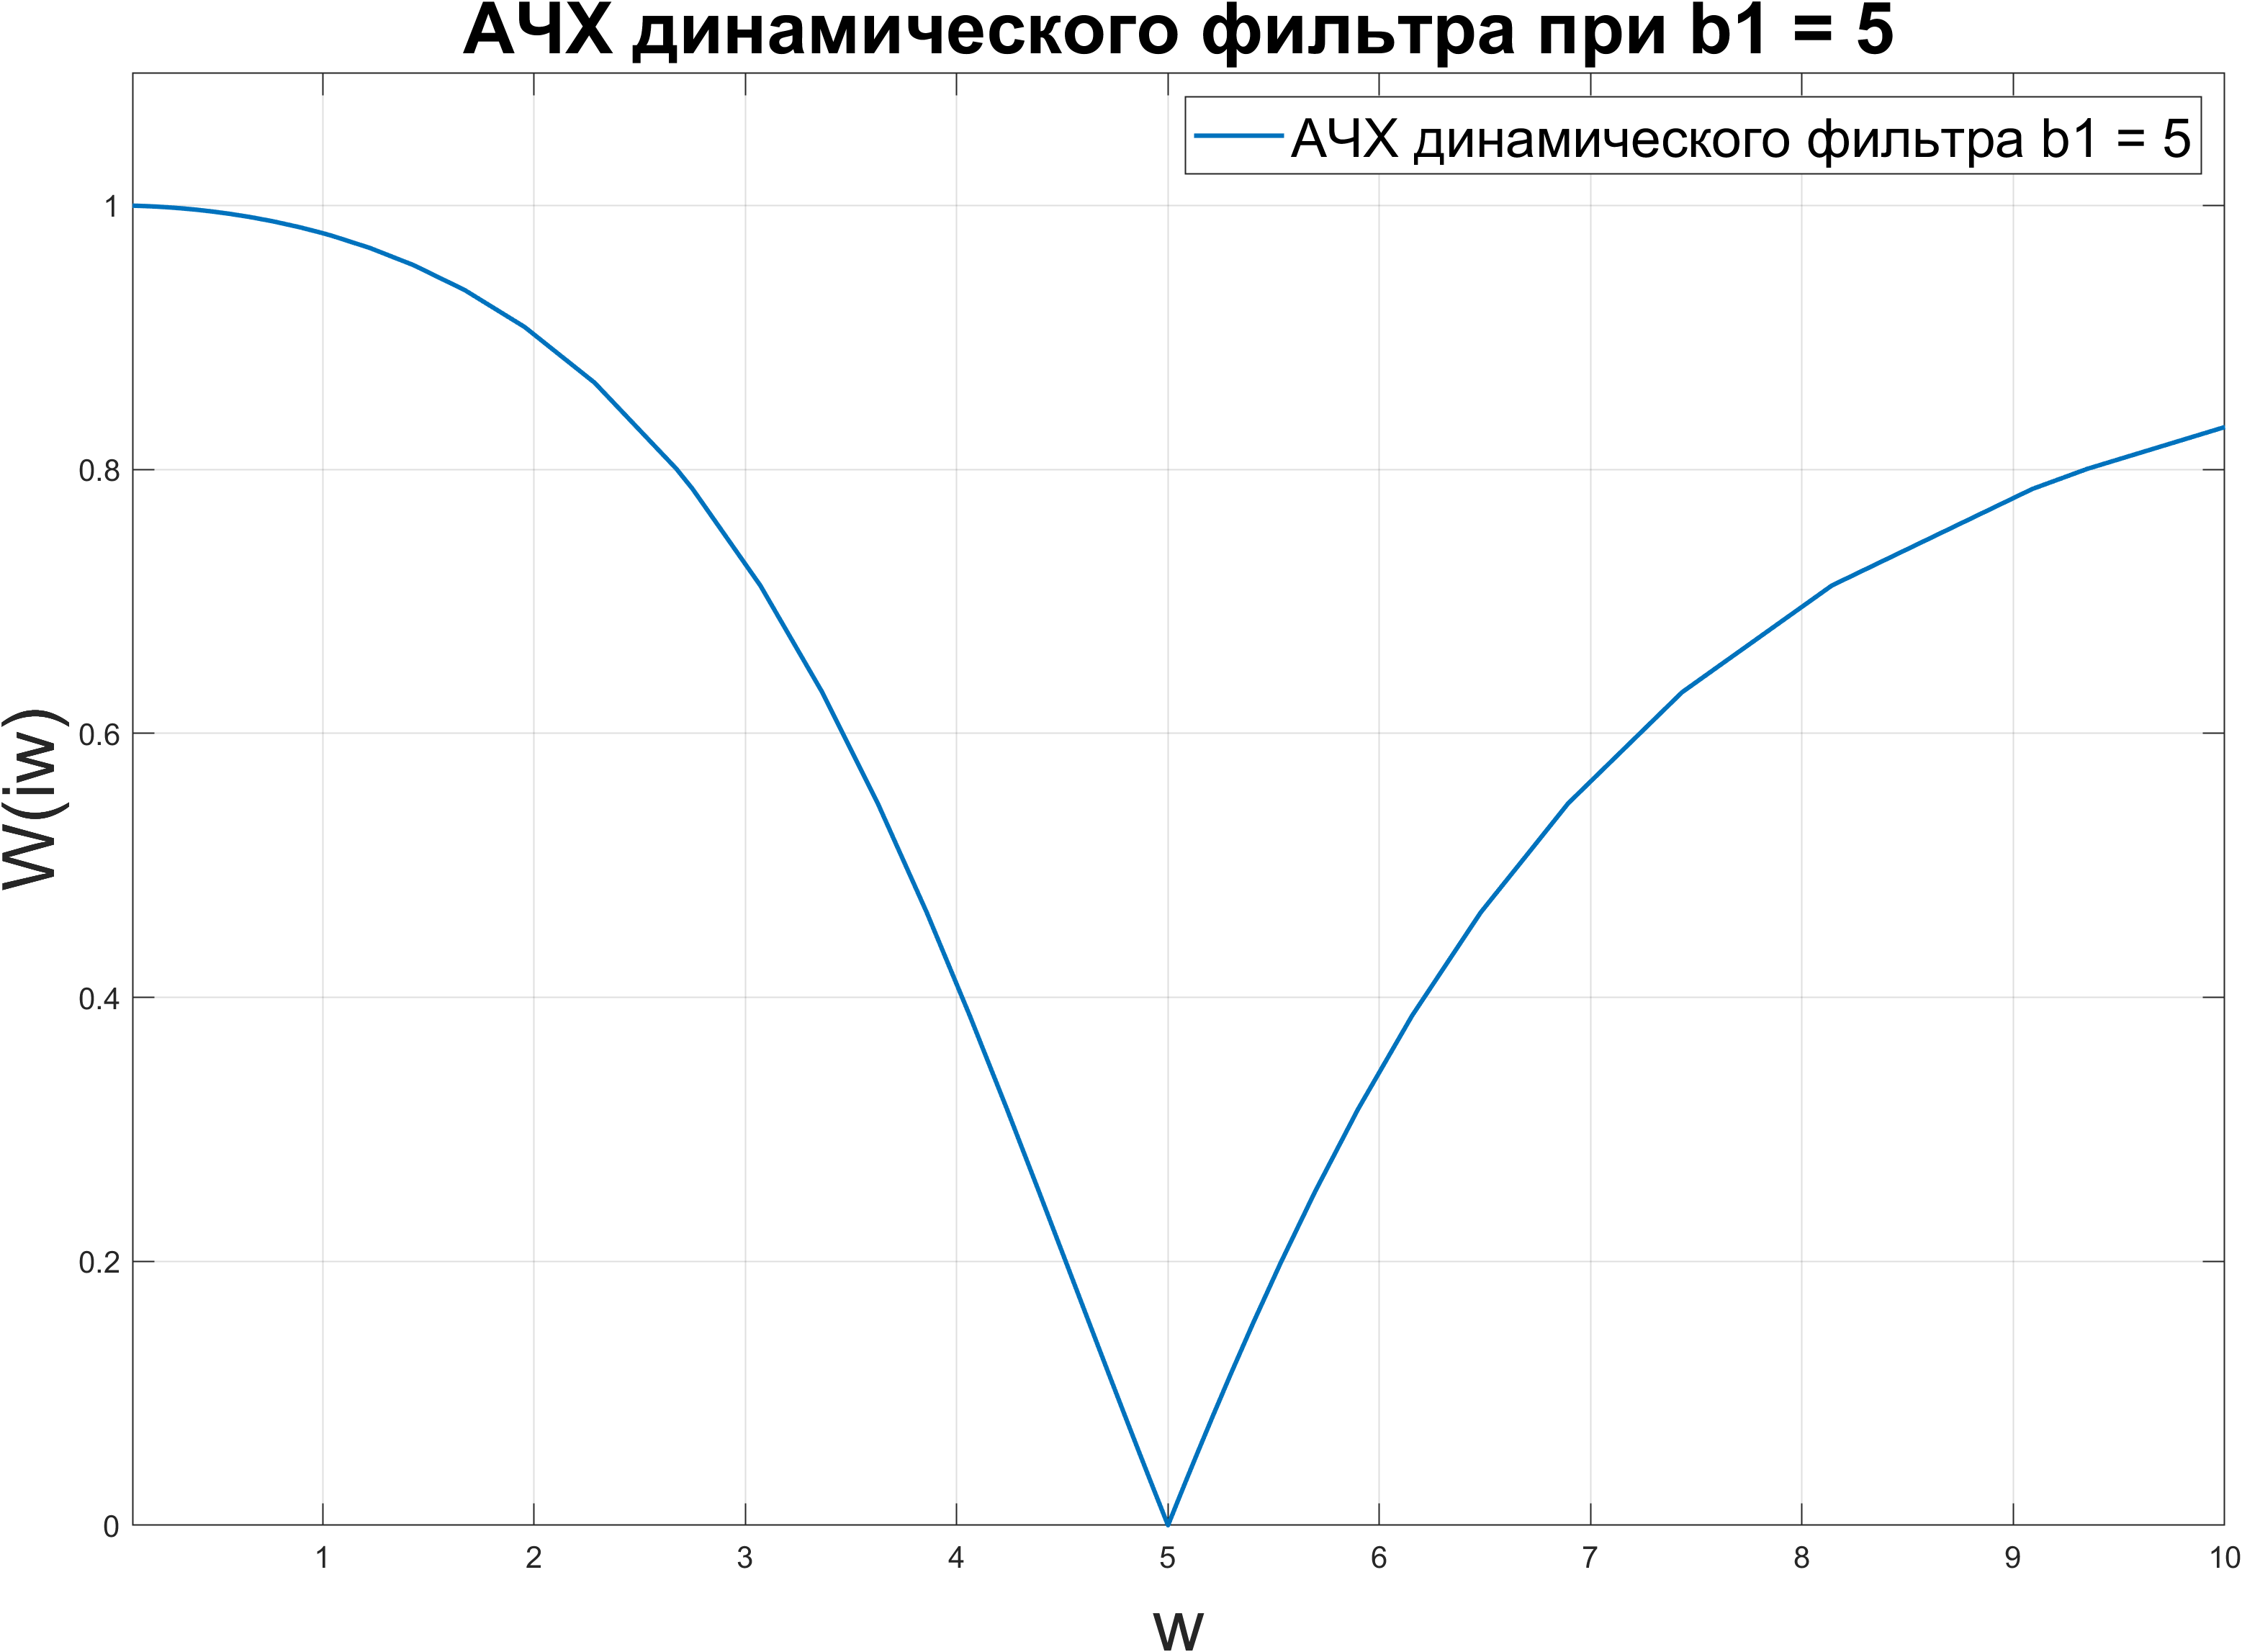
\includegraphics[width=0.83\textwidth, keepaspectratio]{images2/filter_ach_b1_5.png}
    \caption{АЧХ при $b_1 = 5$}
\end{figure}
\newpage

\begin{figure}[H]
    \centering
    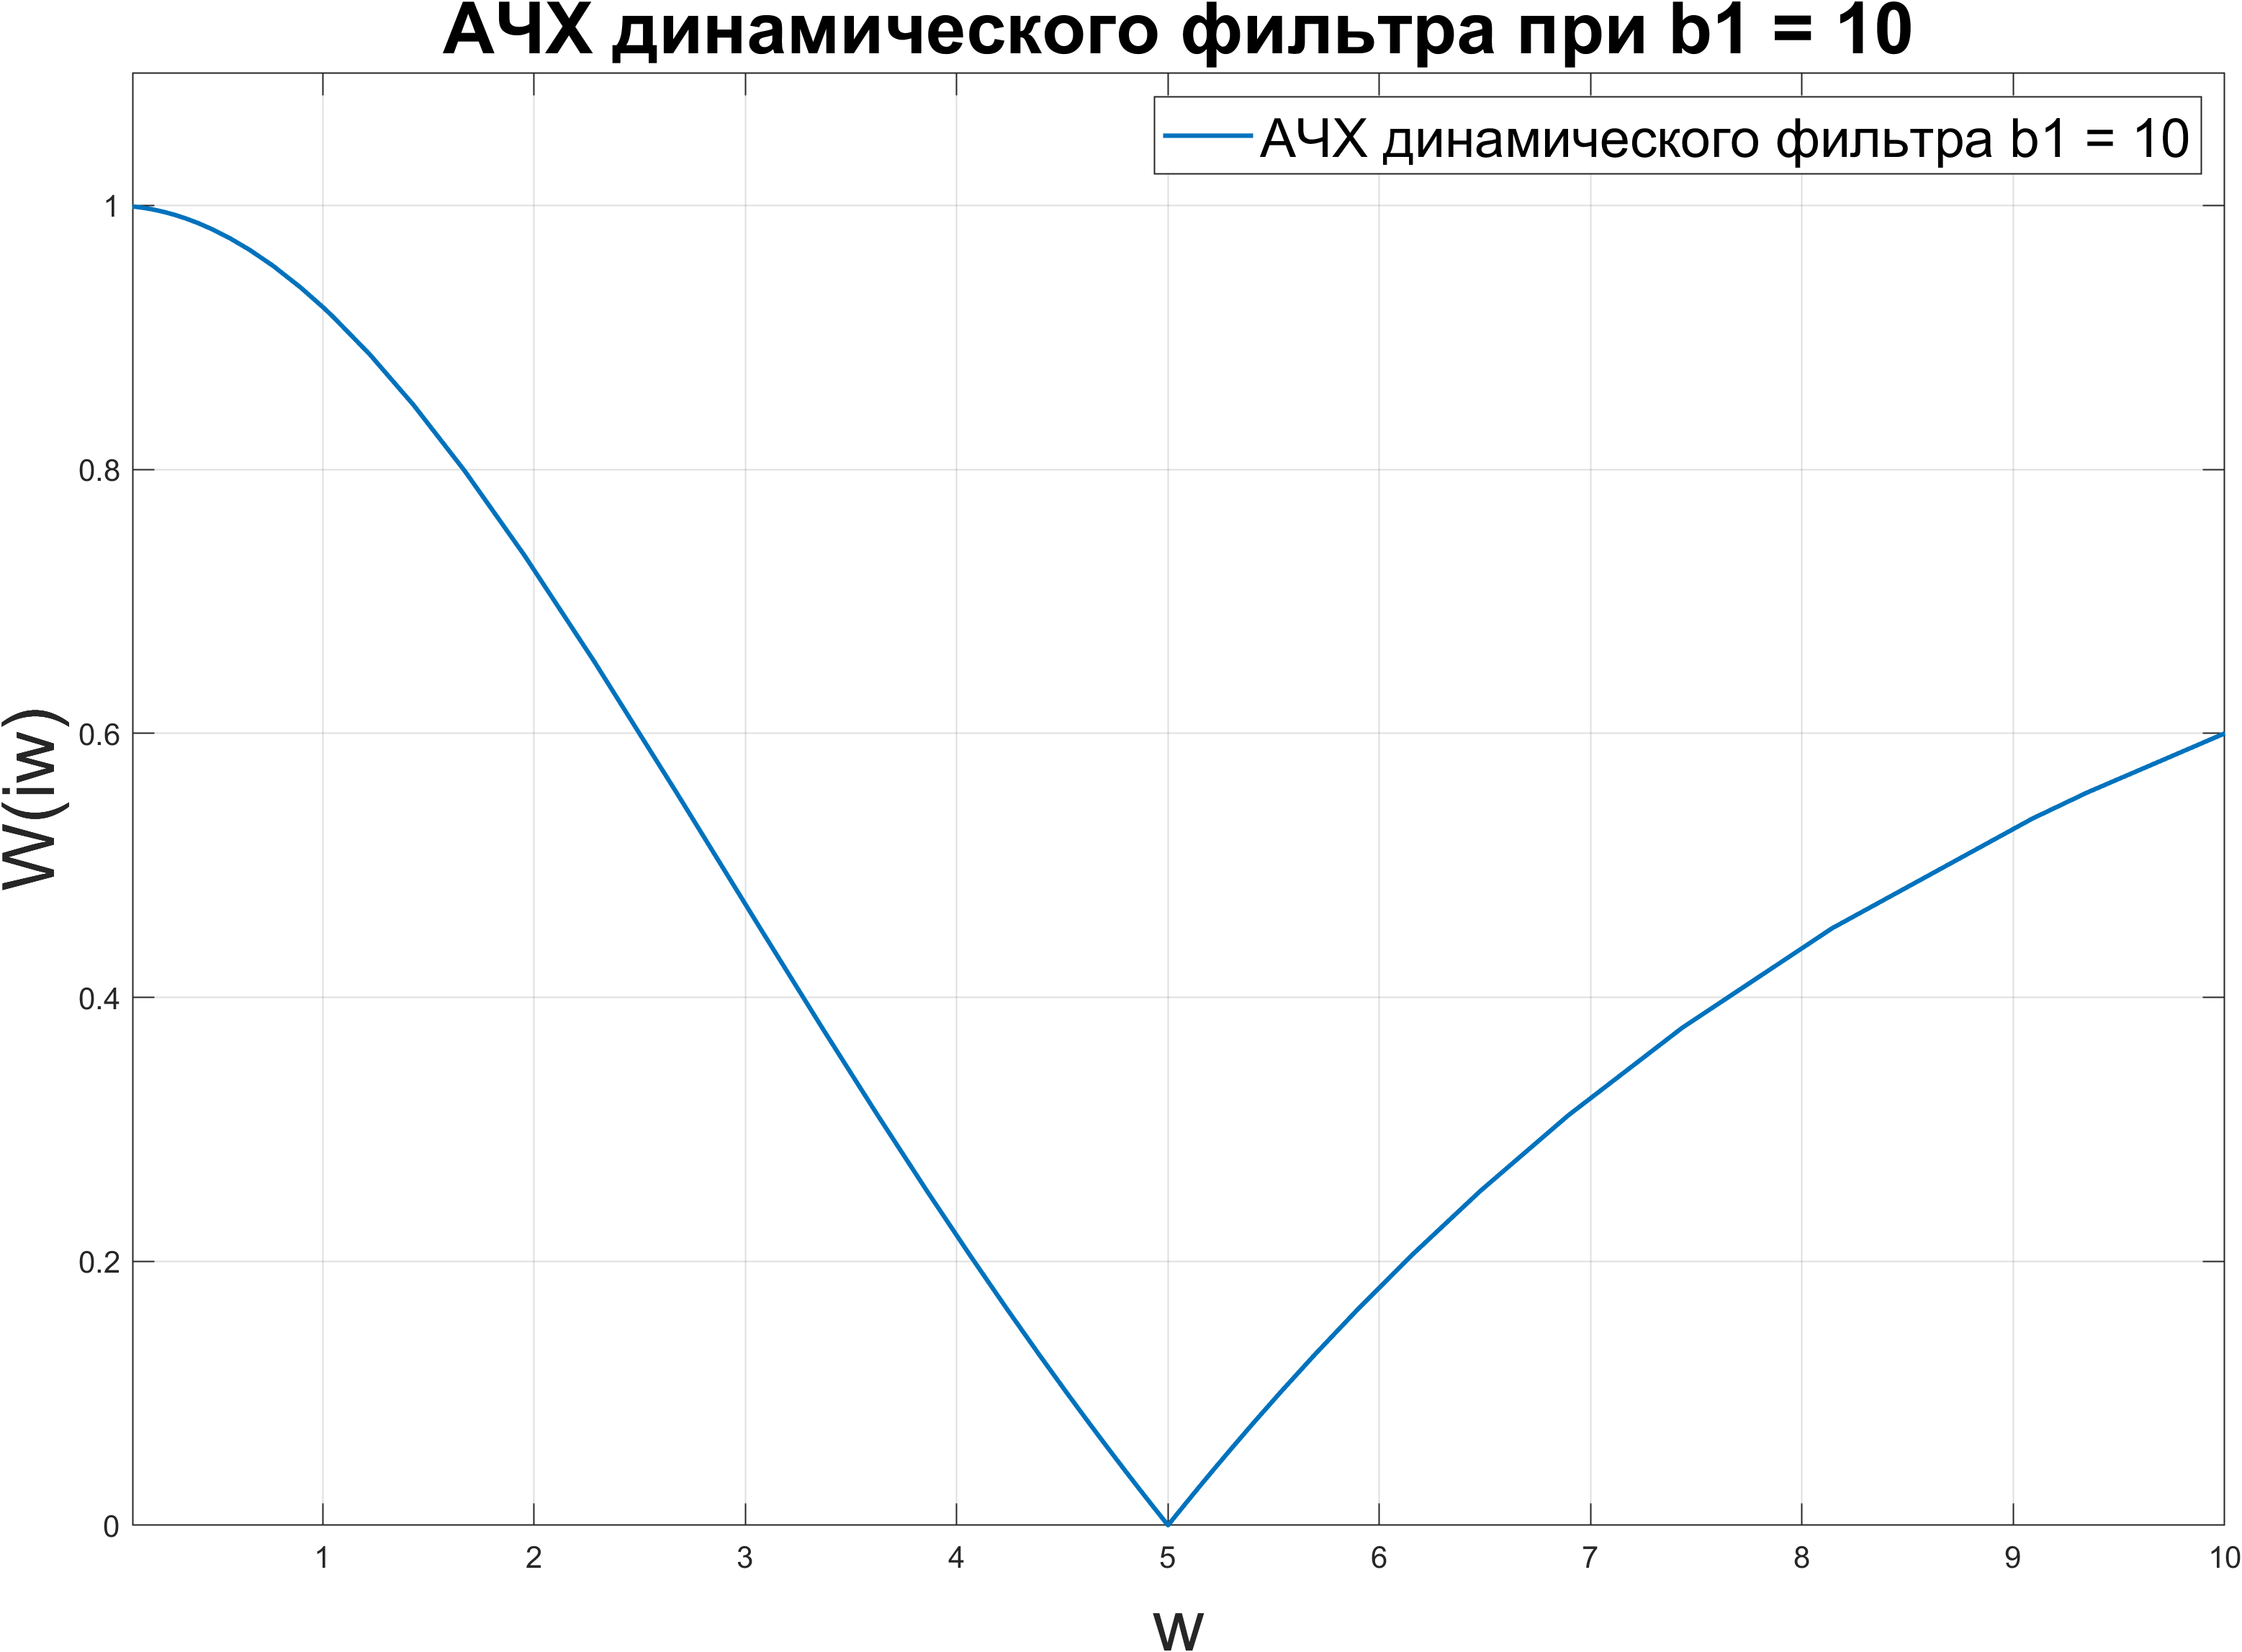
\includegraphics[width=0.92\textwidth, keepaspectratio]{images2/filter_ach_b1_10.png}
    \caption{АЧХ при $b_1 = 10$}
\end{figure}
\begin{figure}[H]
    \centering
    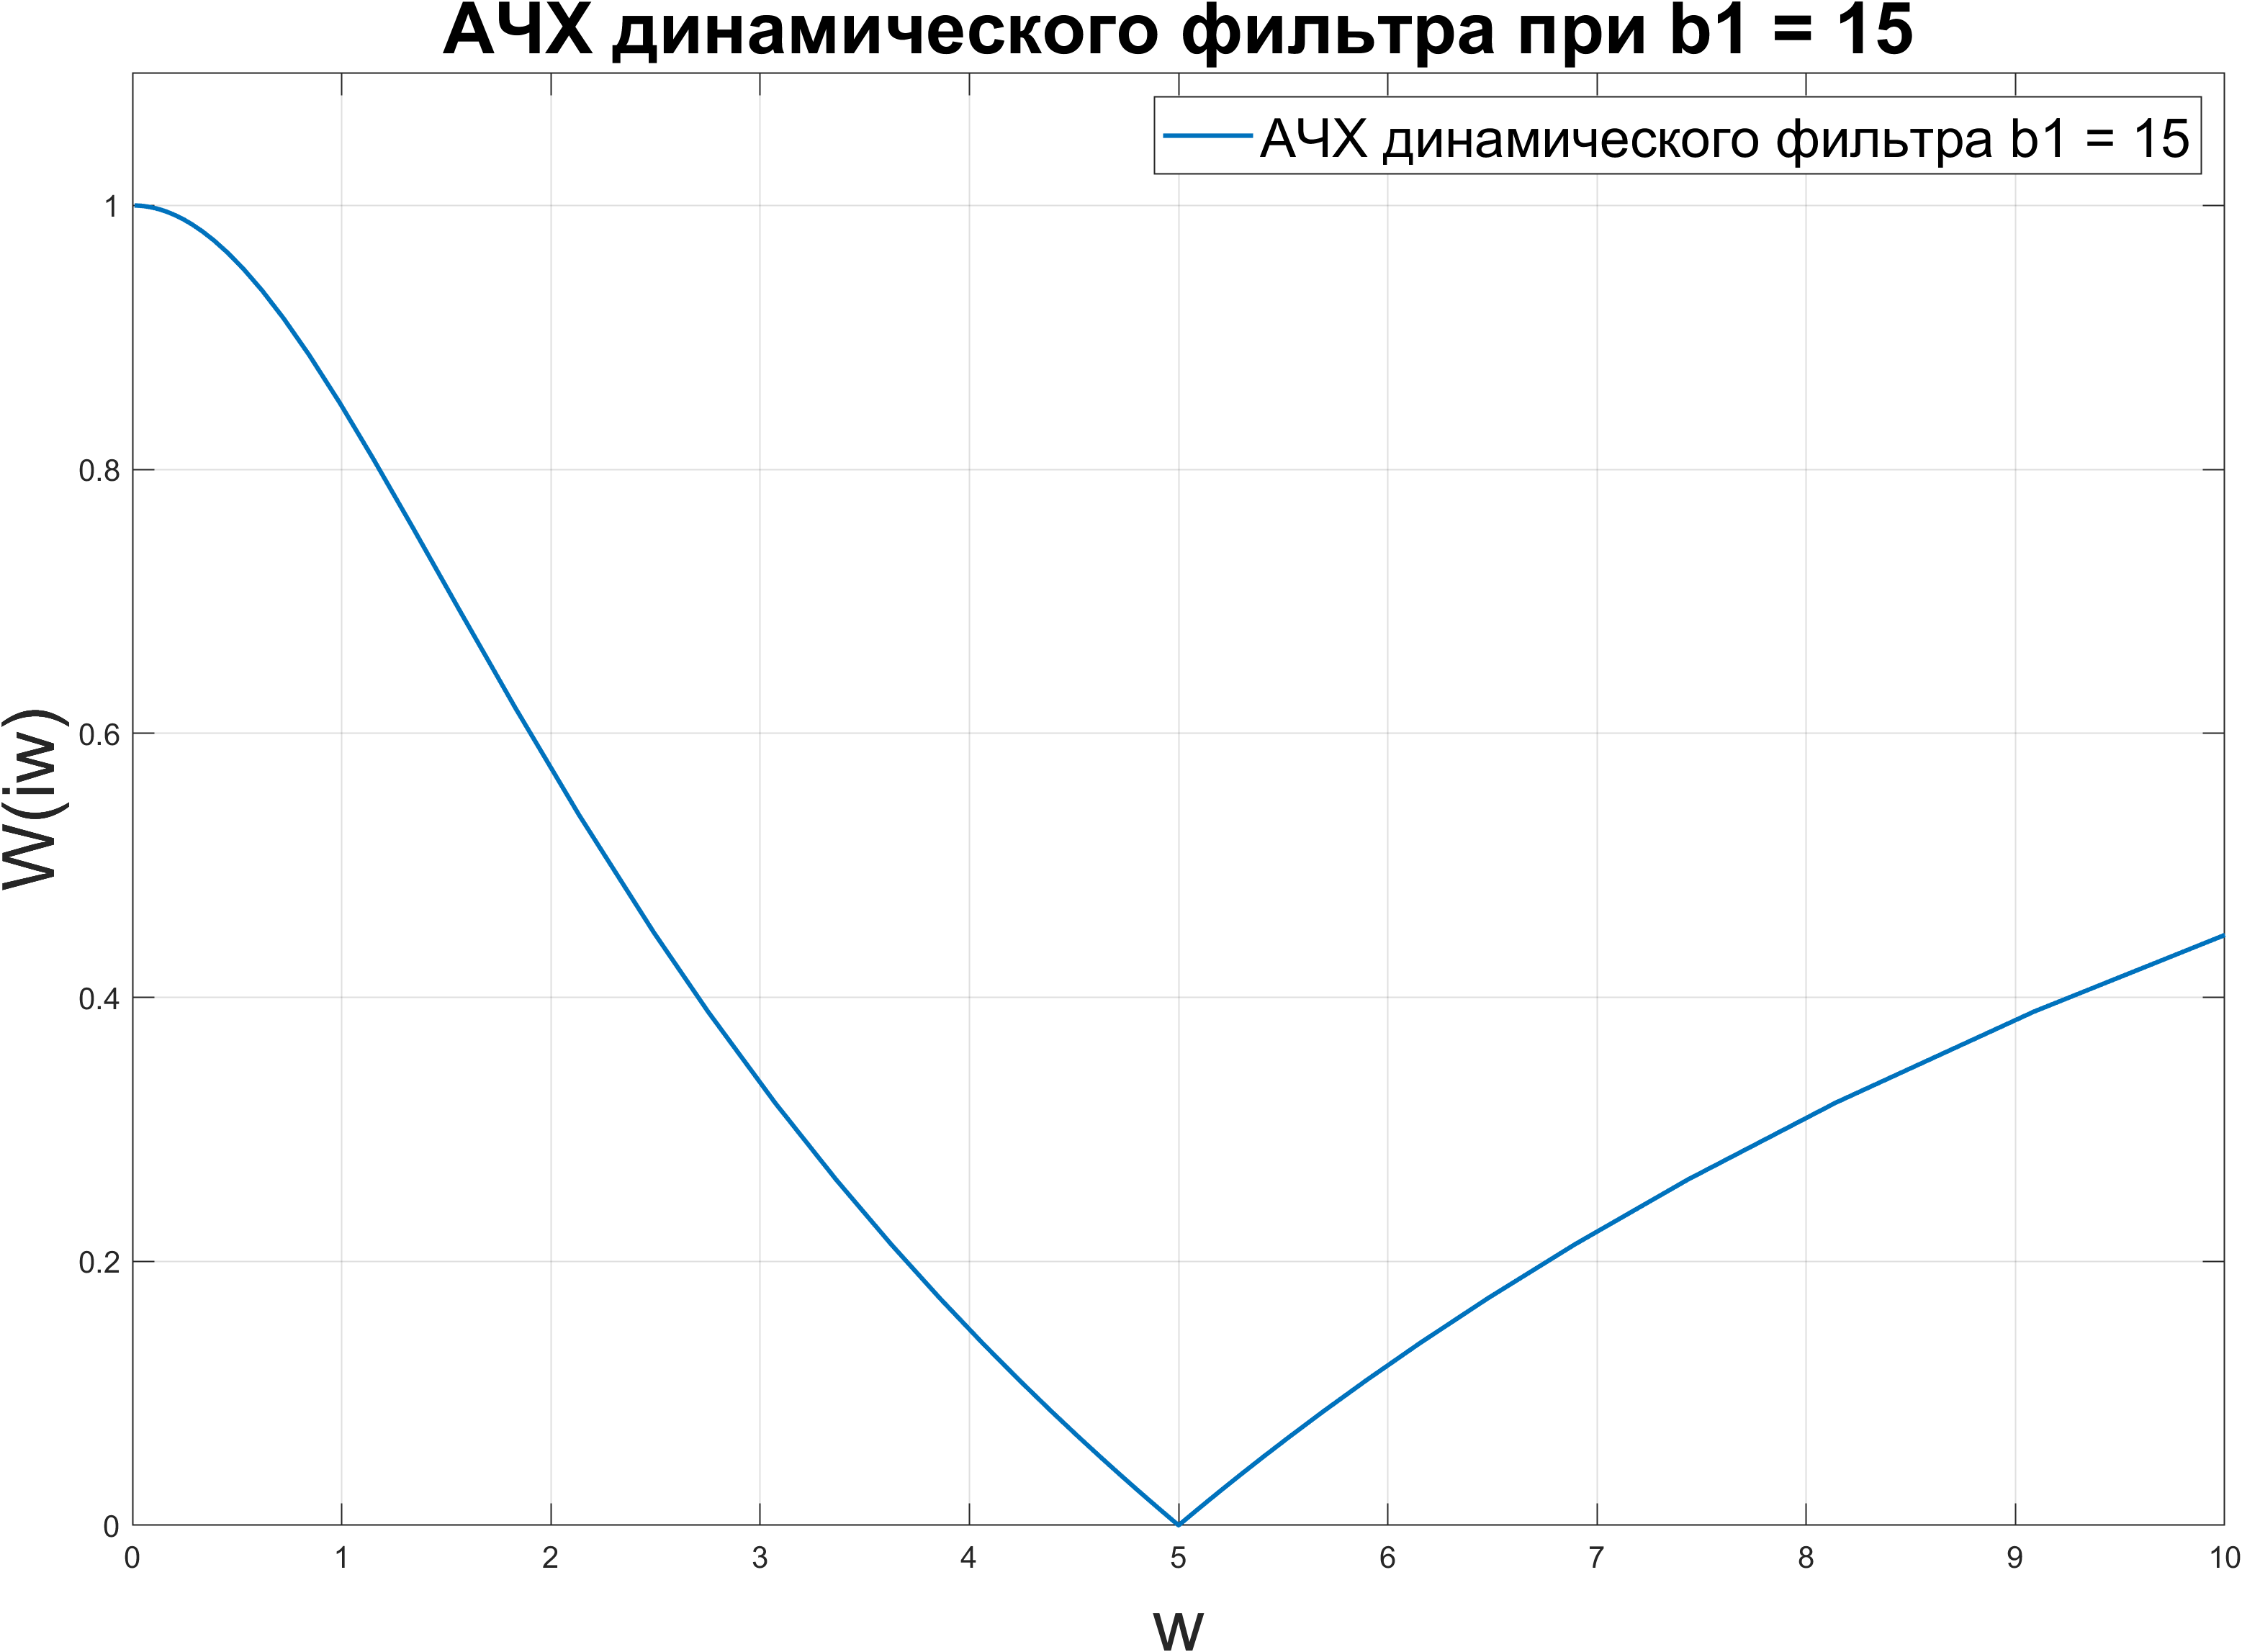
\includegraphics[width=0.92\textwidth, keepaspectratio]{images2/filter_ach_b1_15.png}
    \caption{АЧХ при $b_1 = 15$}
\end{figure}
\newpage

\begin{figure}[H]
    \centering
    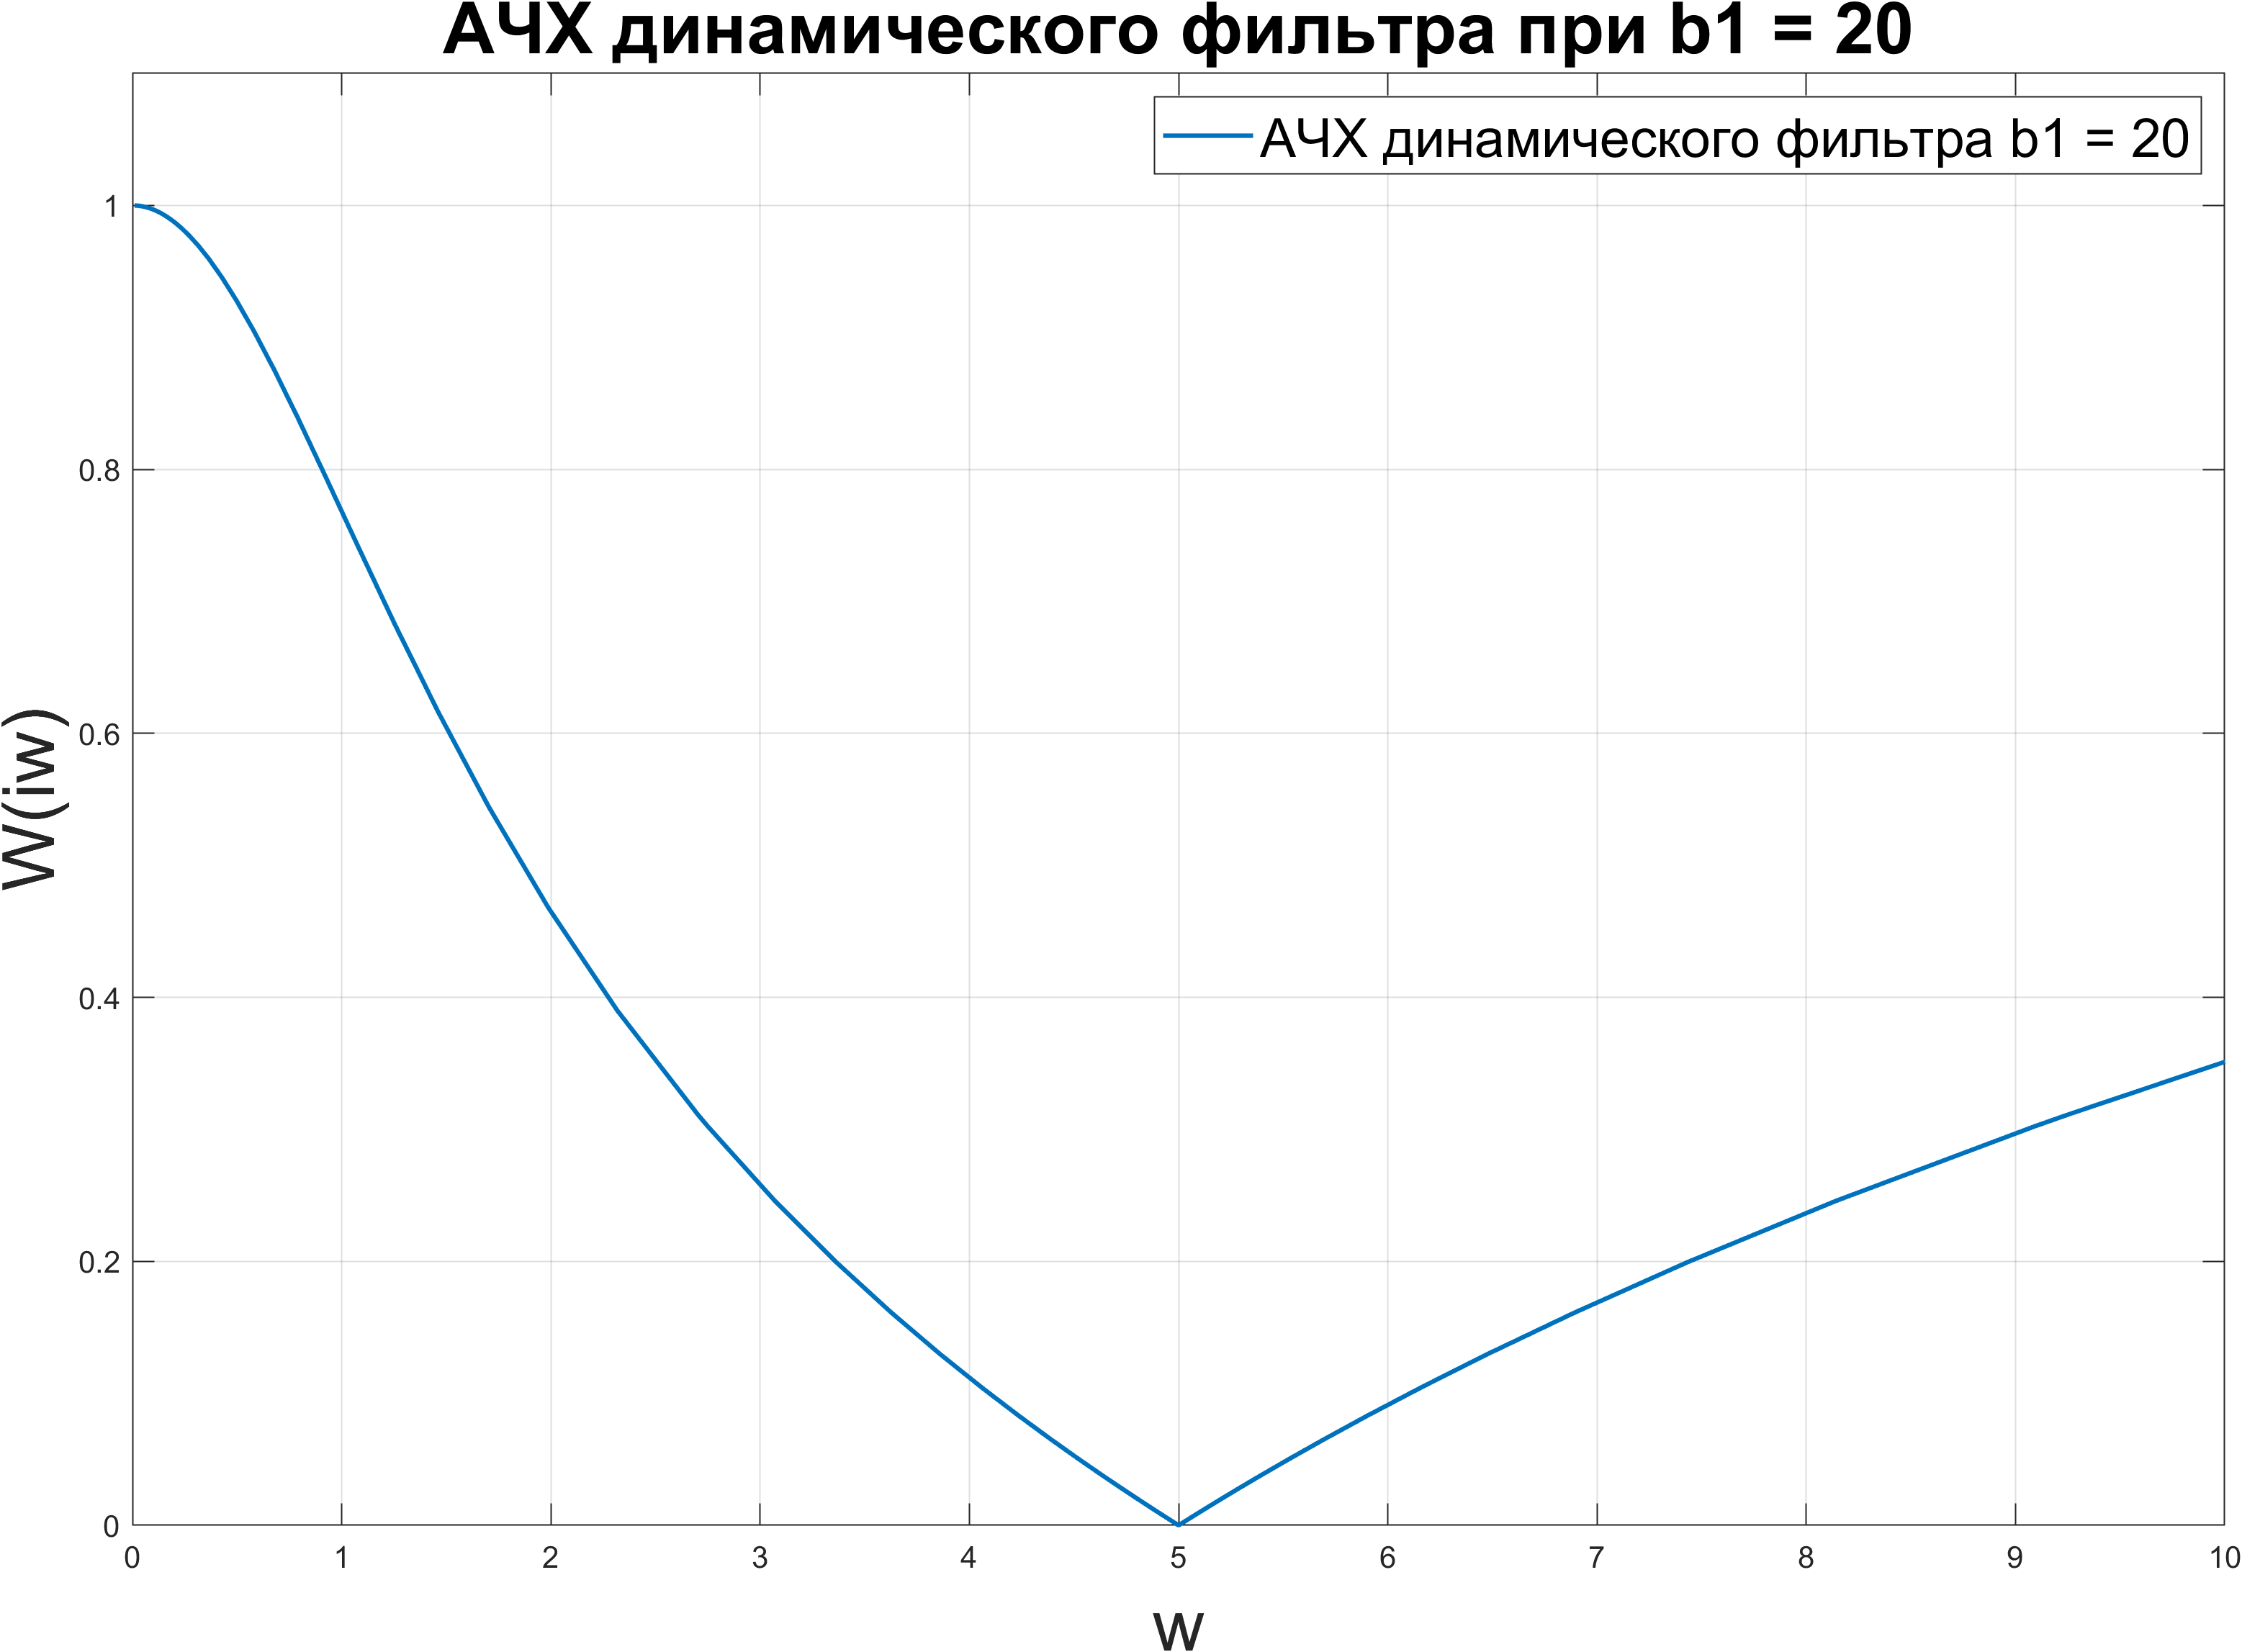
\includegraphics[width=0.92\textwidth, keepaspectratio]{images2/filter_ach_b1_20.png}
    \caption{АЧХ при $b_1 = 20$}
\end{figure}
\begin{figure}[H]
    \centering
    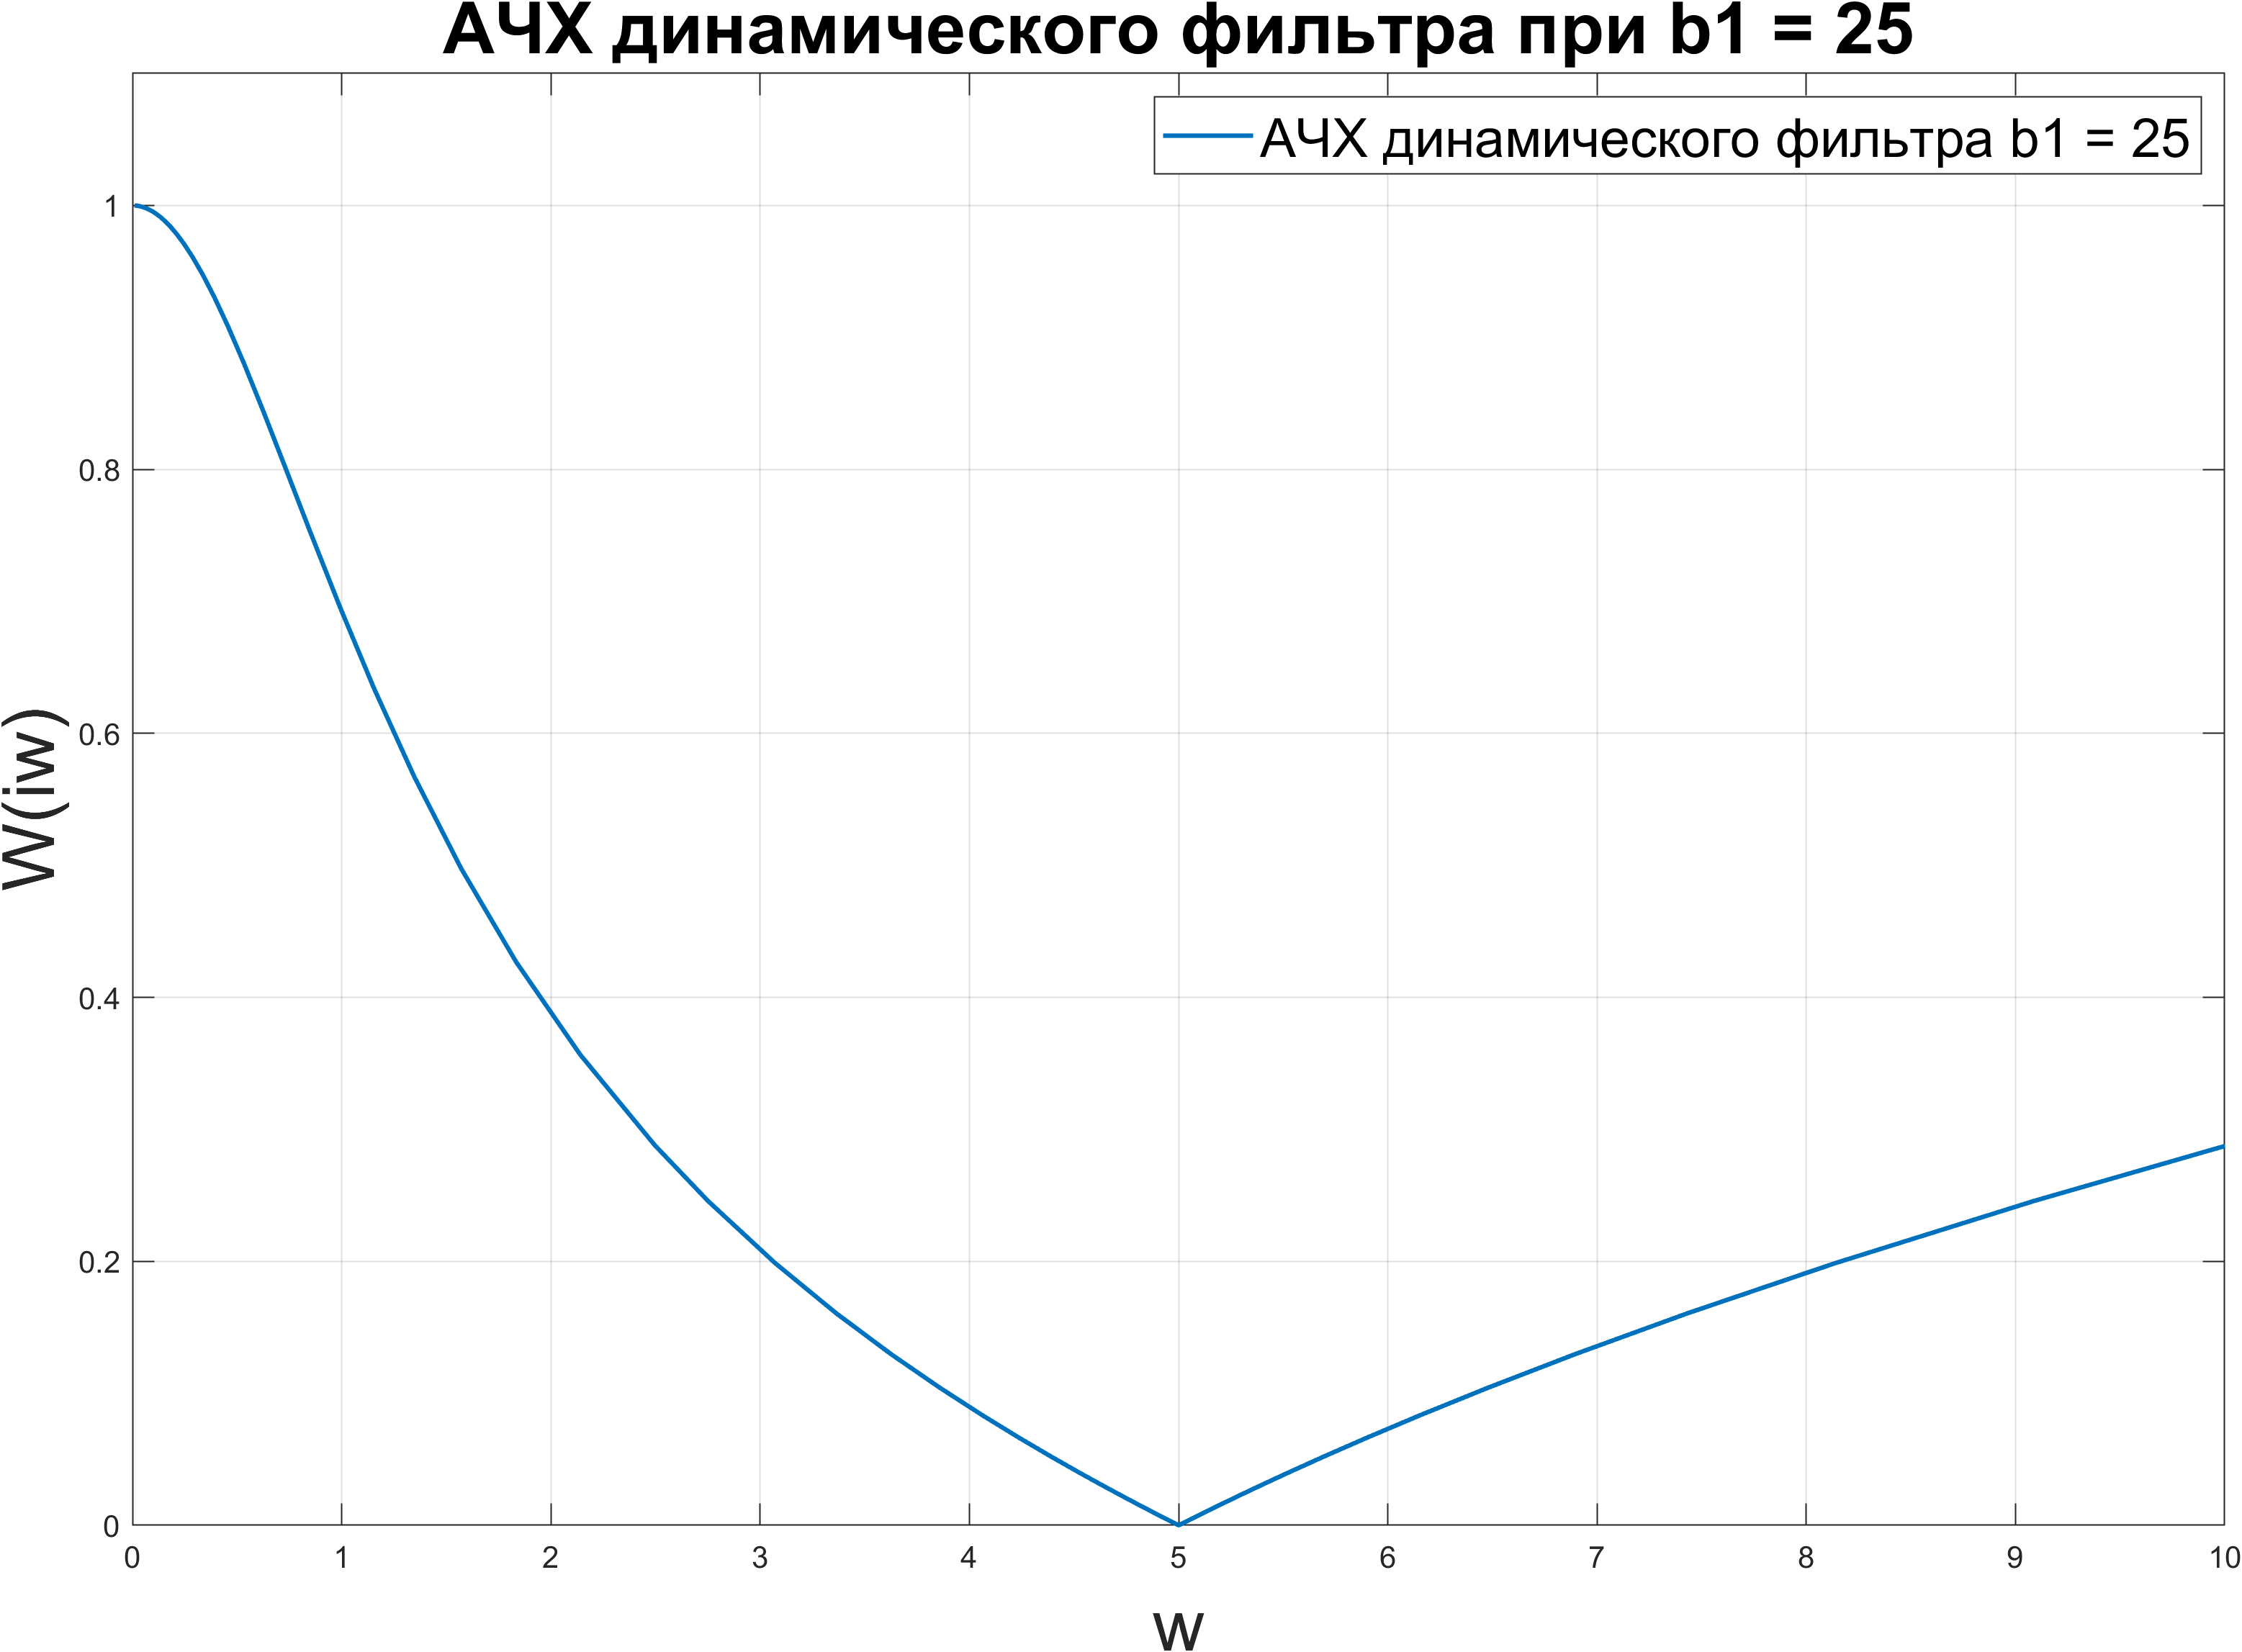
\includegraphics[width=0.92\textwidth, keepaspectratio]{images2/filter_ach_b1_25.png}
    \caption{АЧХ при $b_1 = 25$}
\end{figure}
\newpage

Демонстрация фильтрации сигнала:
\begin{figure}[H]
    \centering
    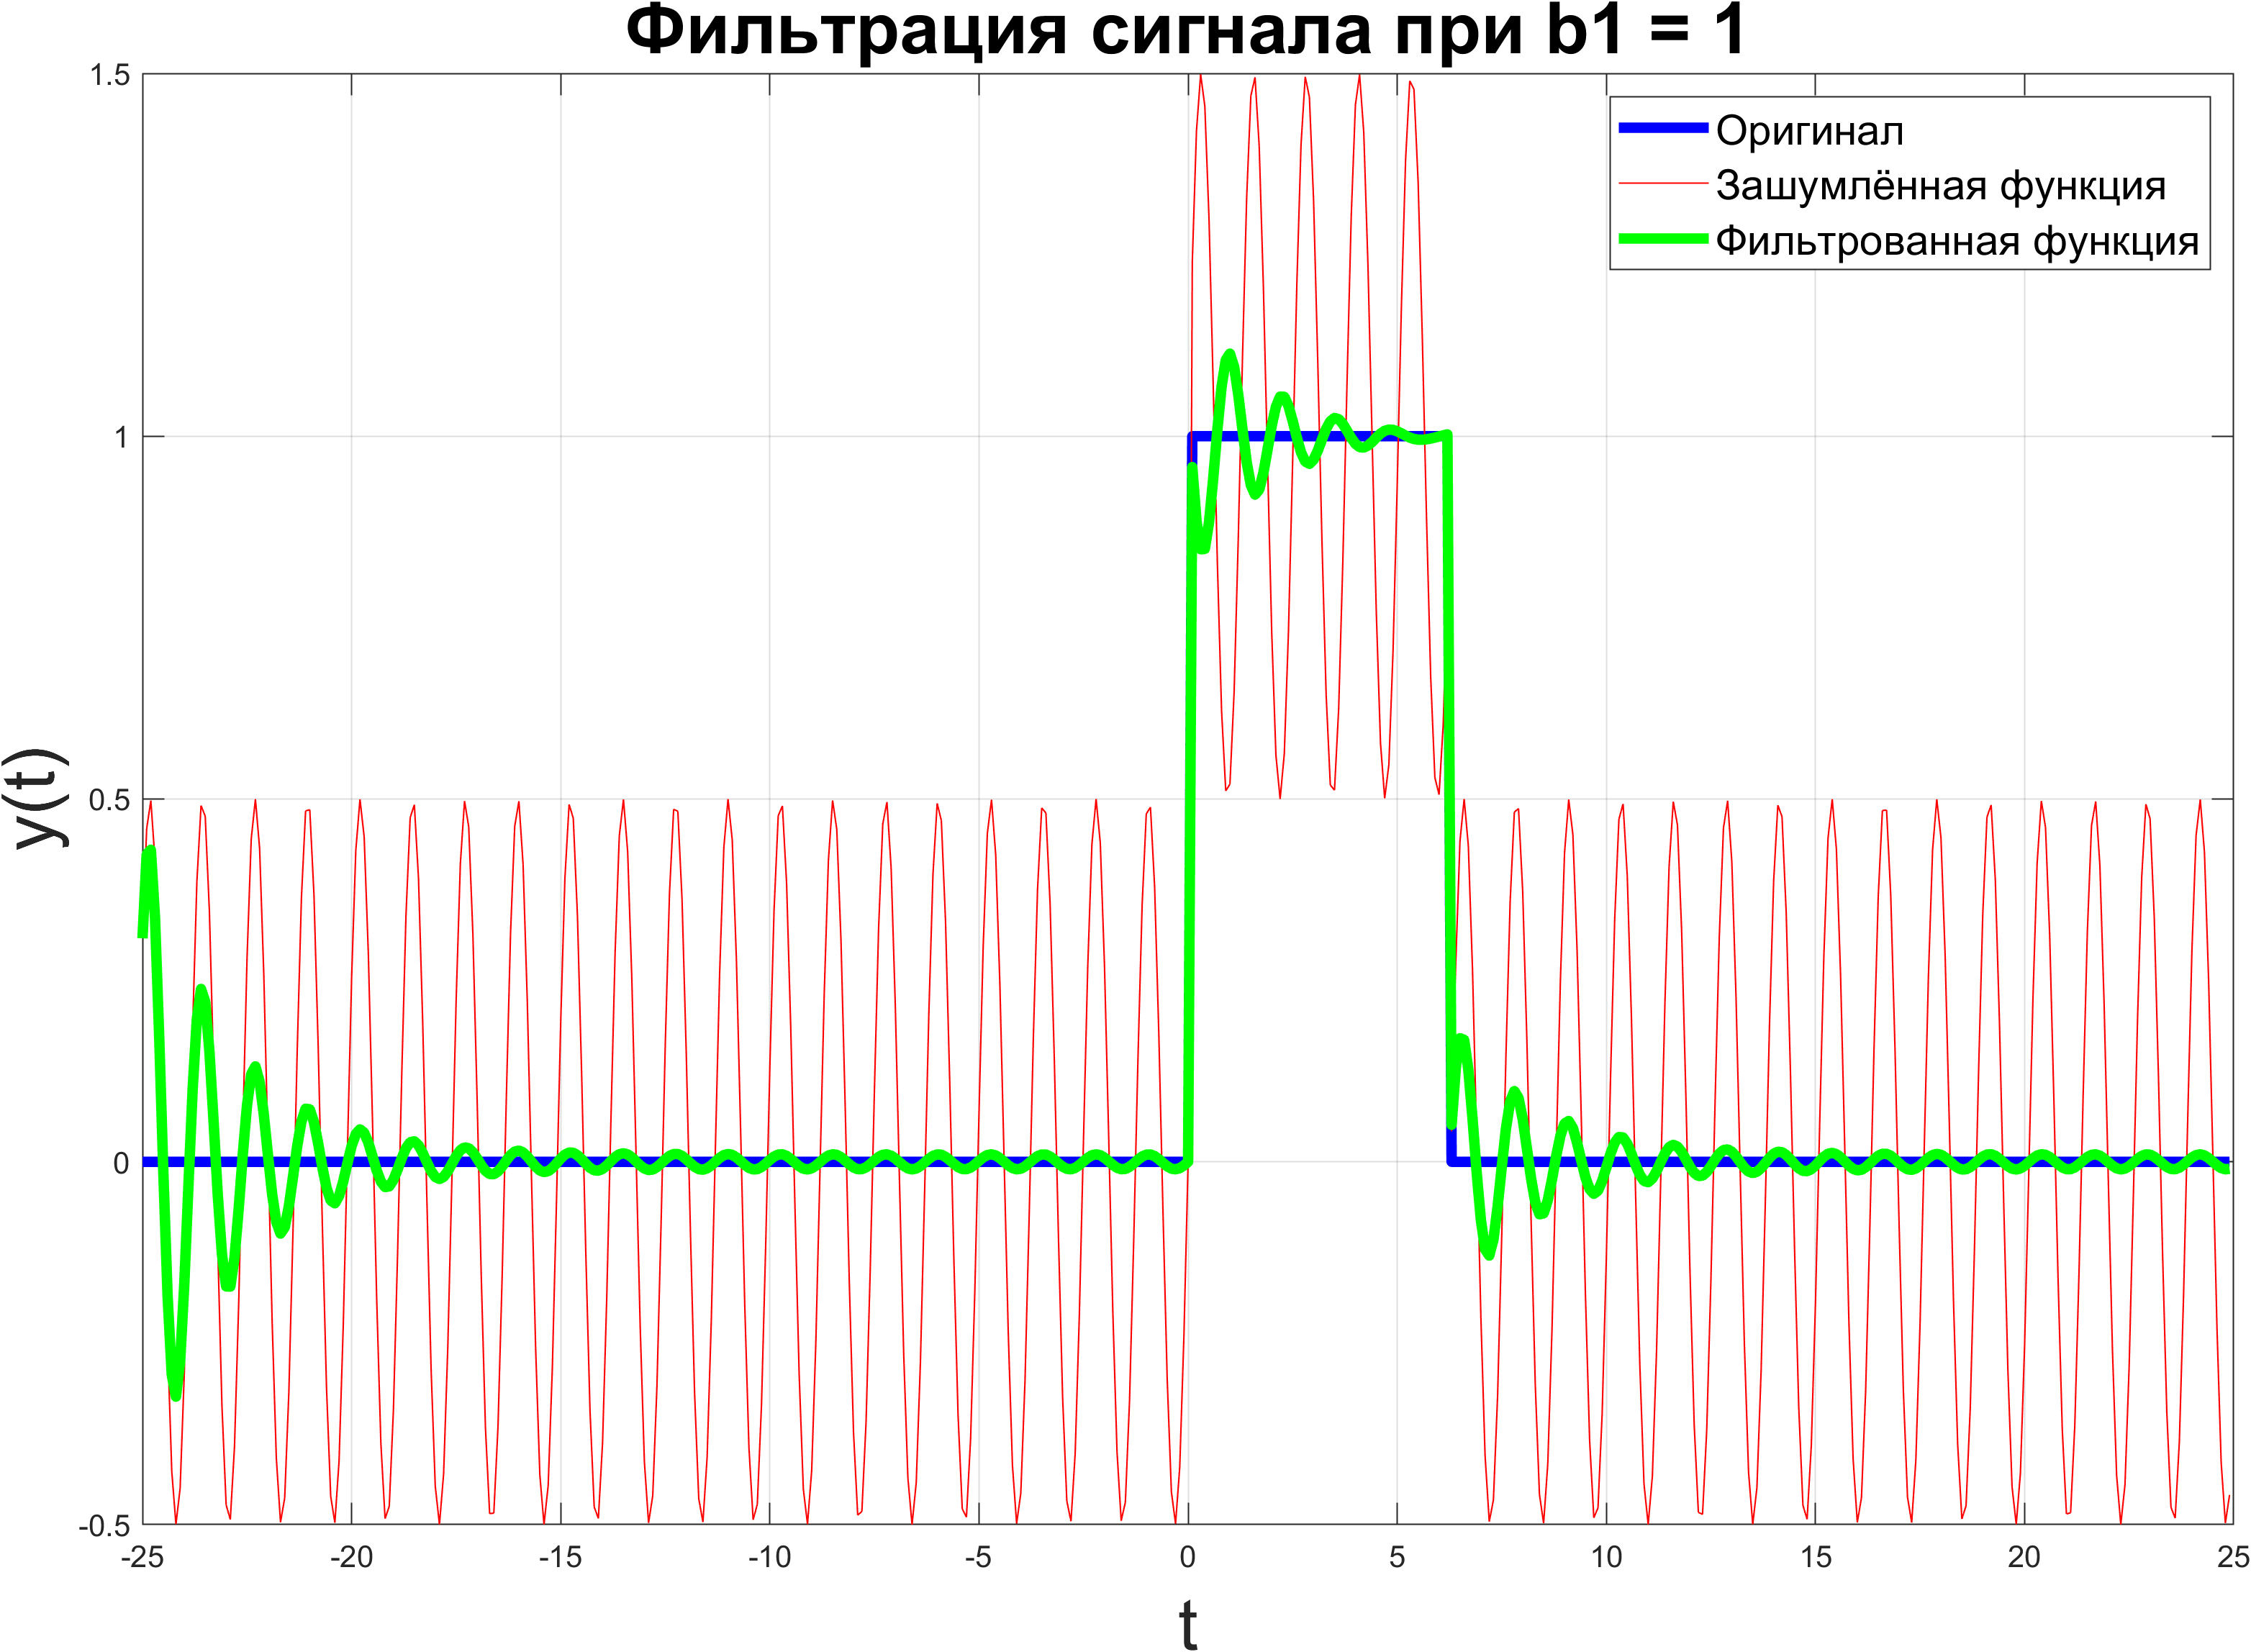
\includegraphics[width=0.85\textwidth, keepaspectratio]{images2/filter_b1_1.png}
    \caption{Фильтрация при $b_1 = 1$}
\end{figure}
\begin{figure}[H]
    \centering
    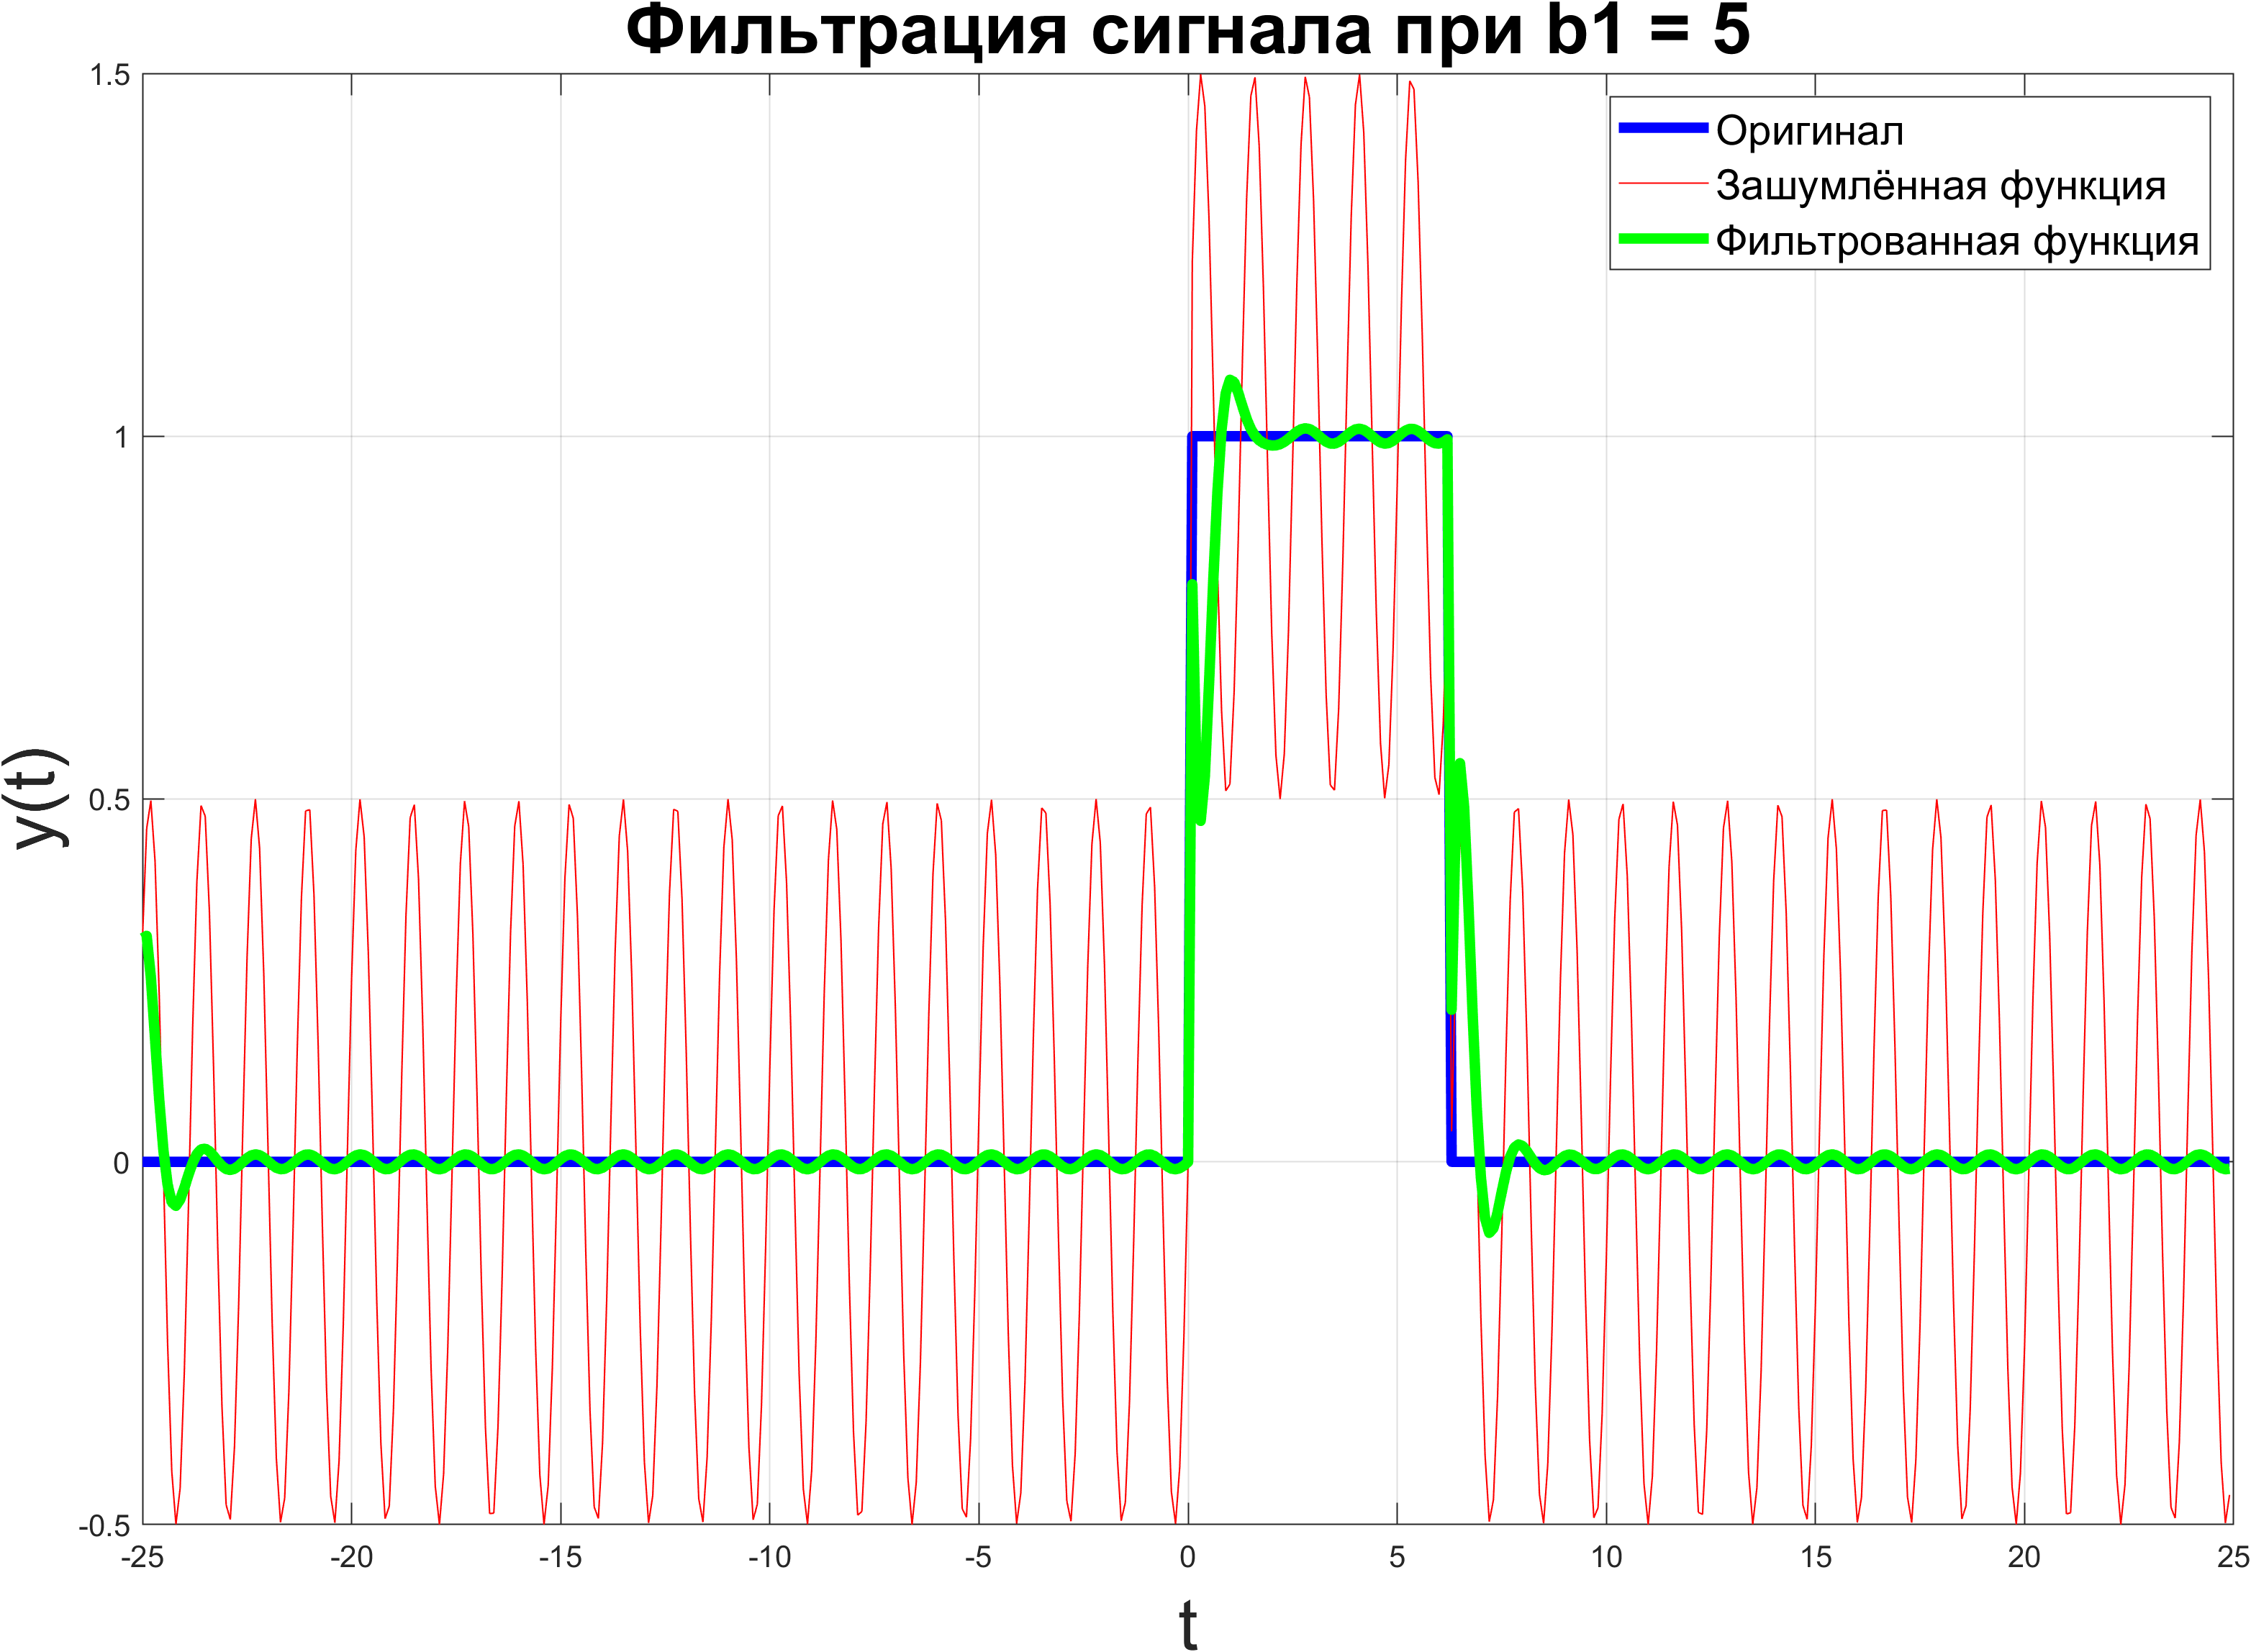
\includegraphics[width=0.85\textwidth, keepaspectratio]{images2/filter_b1_5.png}
    \caption{Фильтрация при $b_1 = 5$}
\end{figure}
\newpage

\begin{figure}[H]
    \centering
    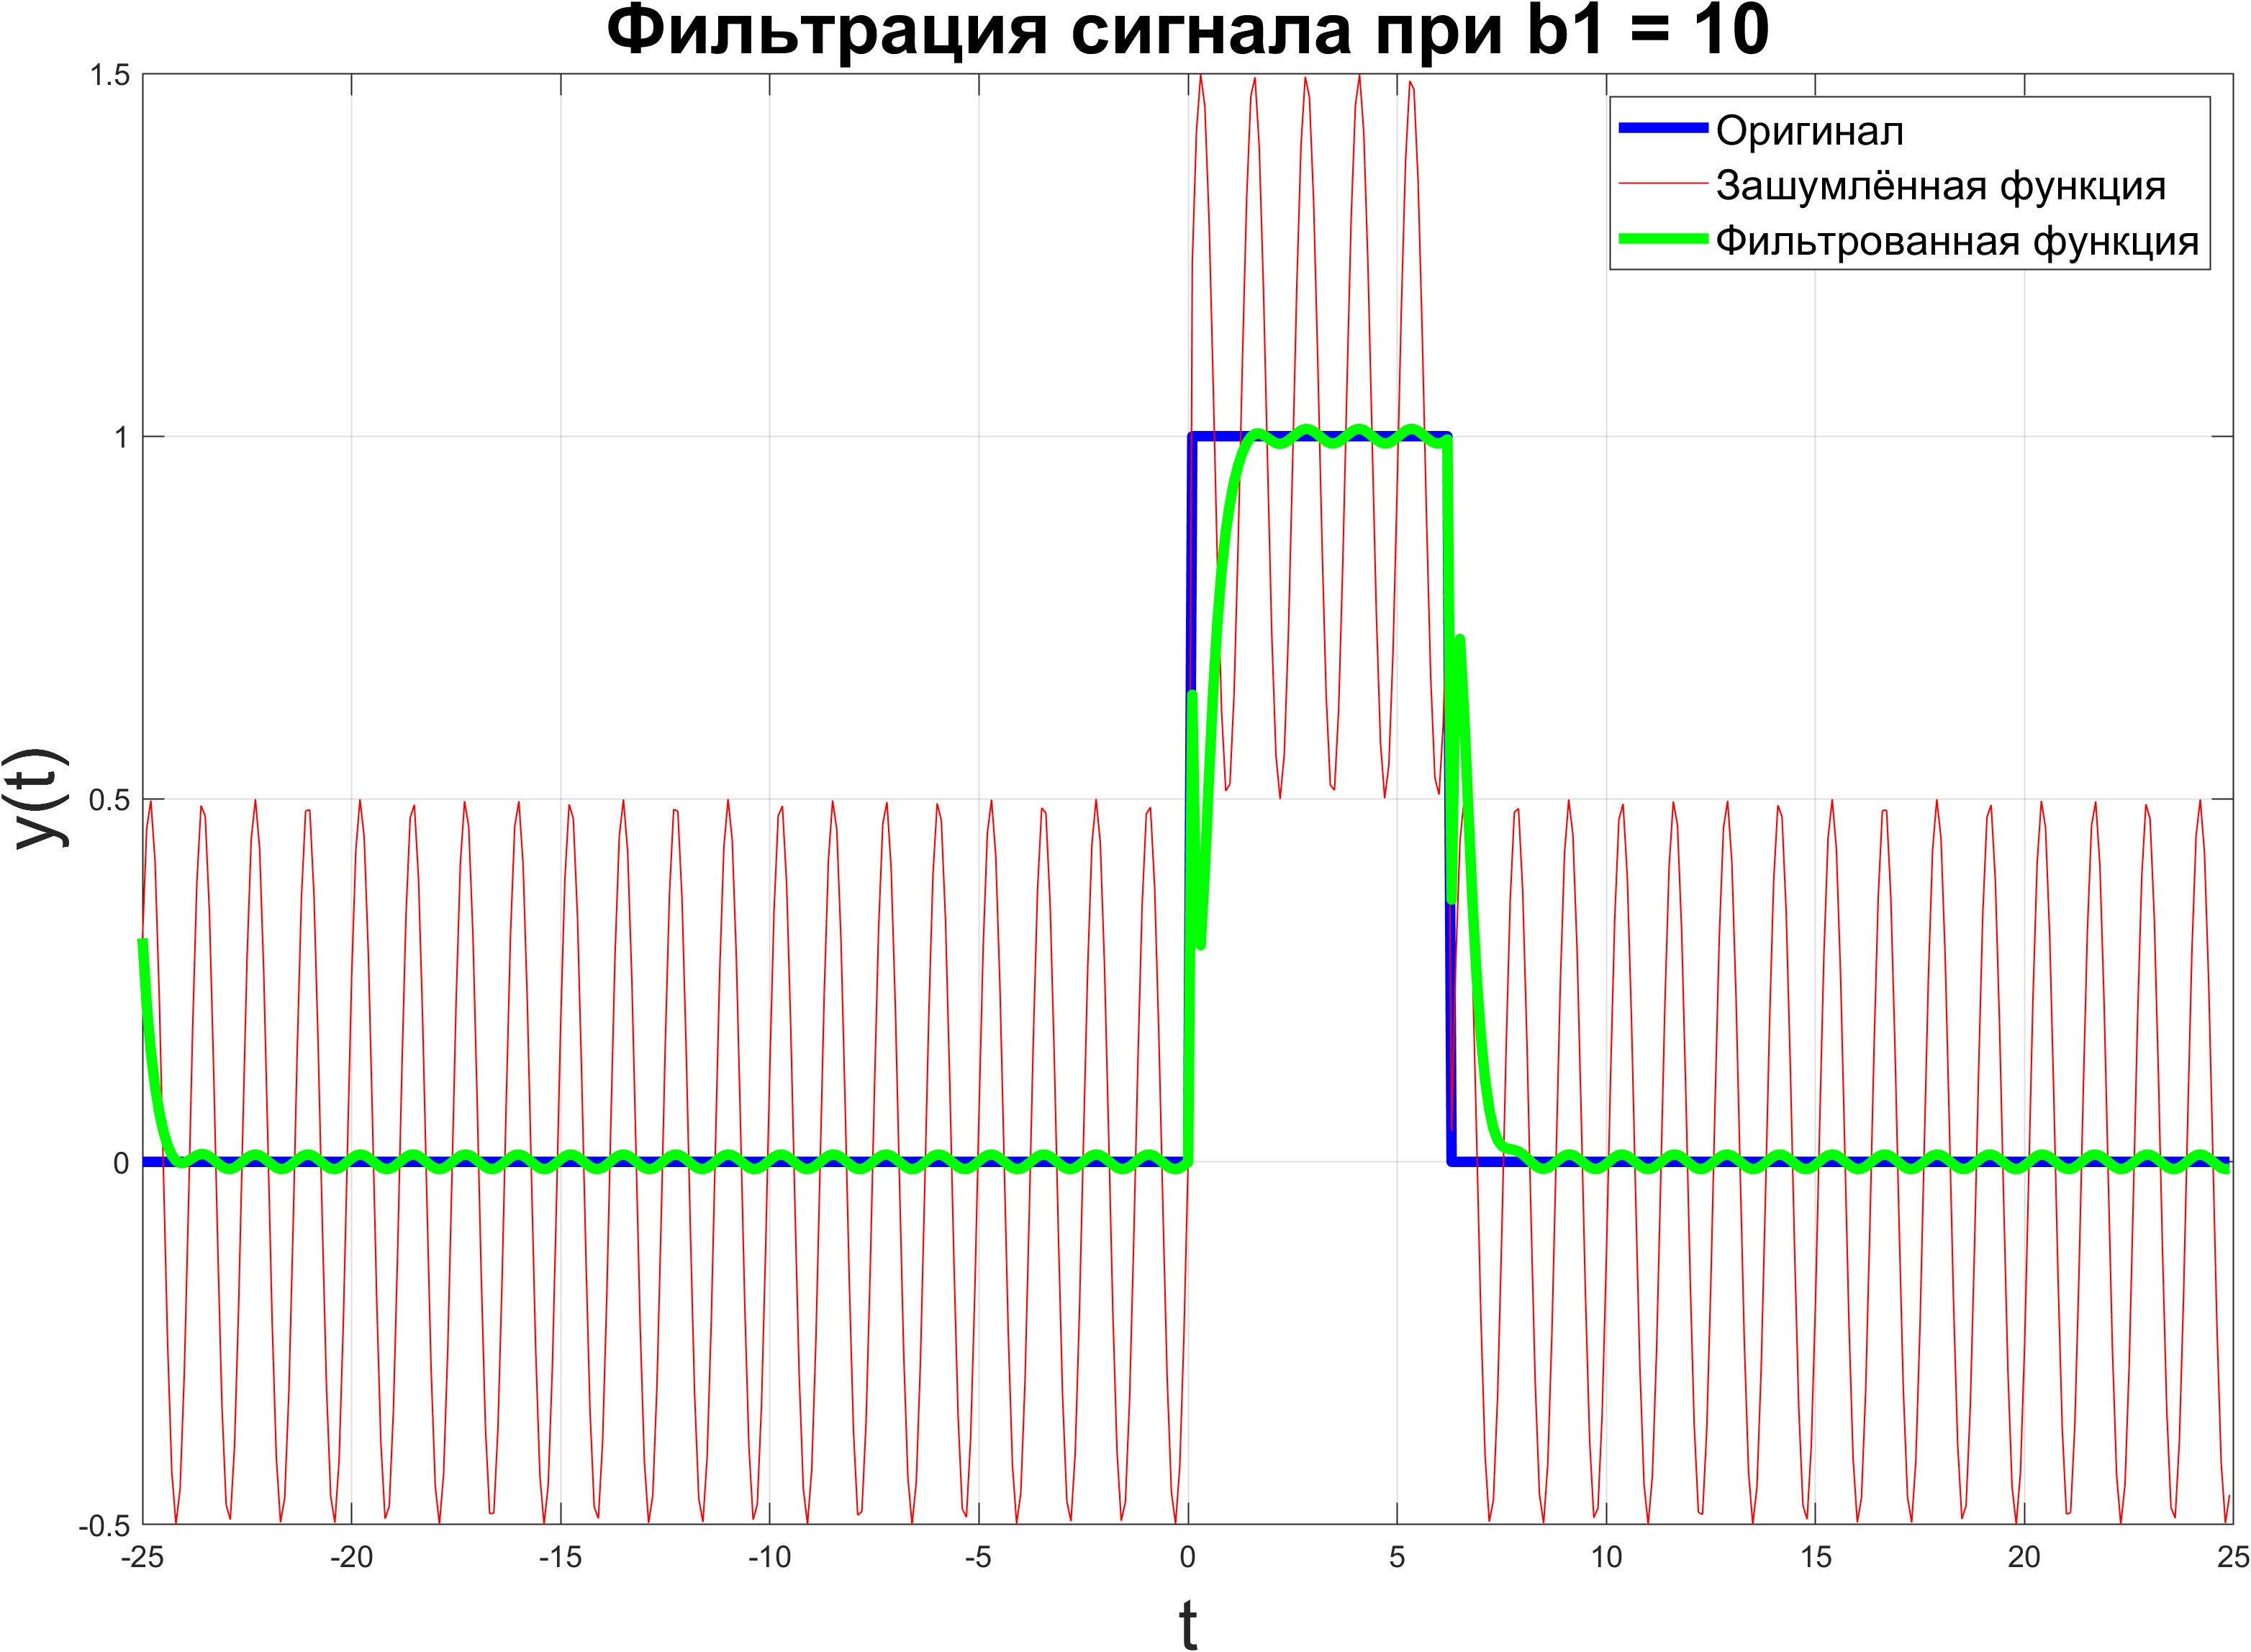
\includegraphics[width=0.92\textwidth, keepaspectratio]{images2/filter_b1_10.png}
    \caption{Фильтрация при $b_1 = 10$}
\end{figure}
\begin{figure}[H]
    \centering
    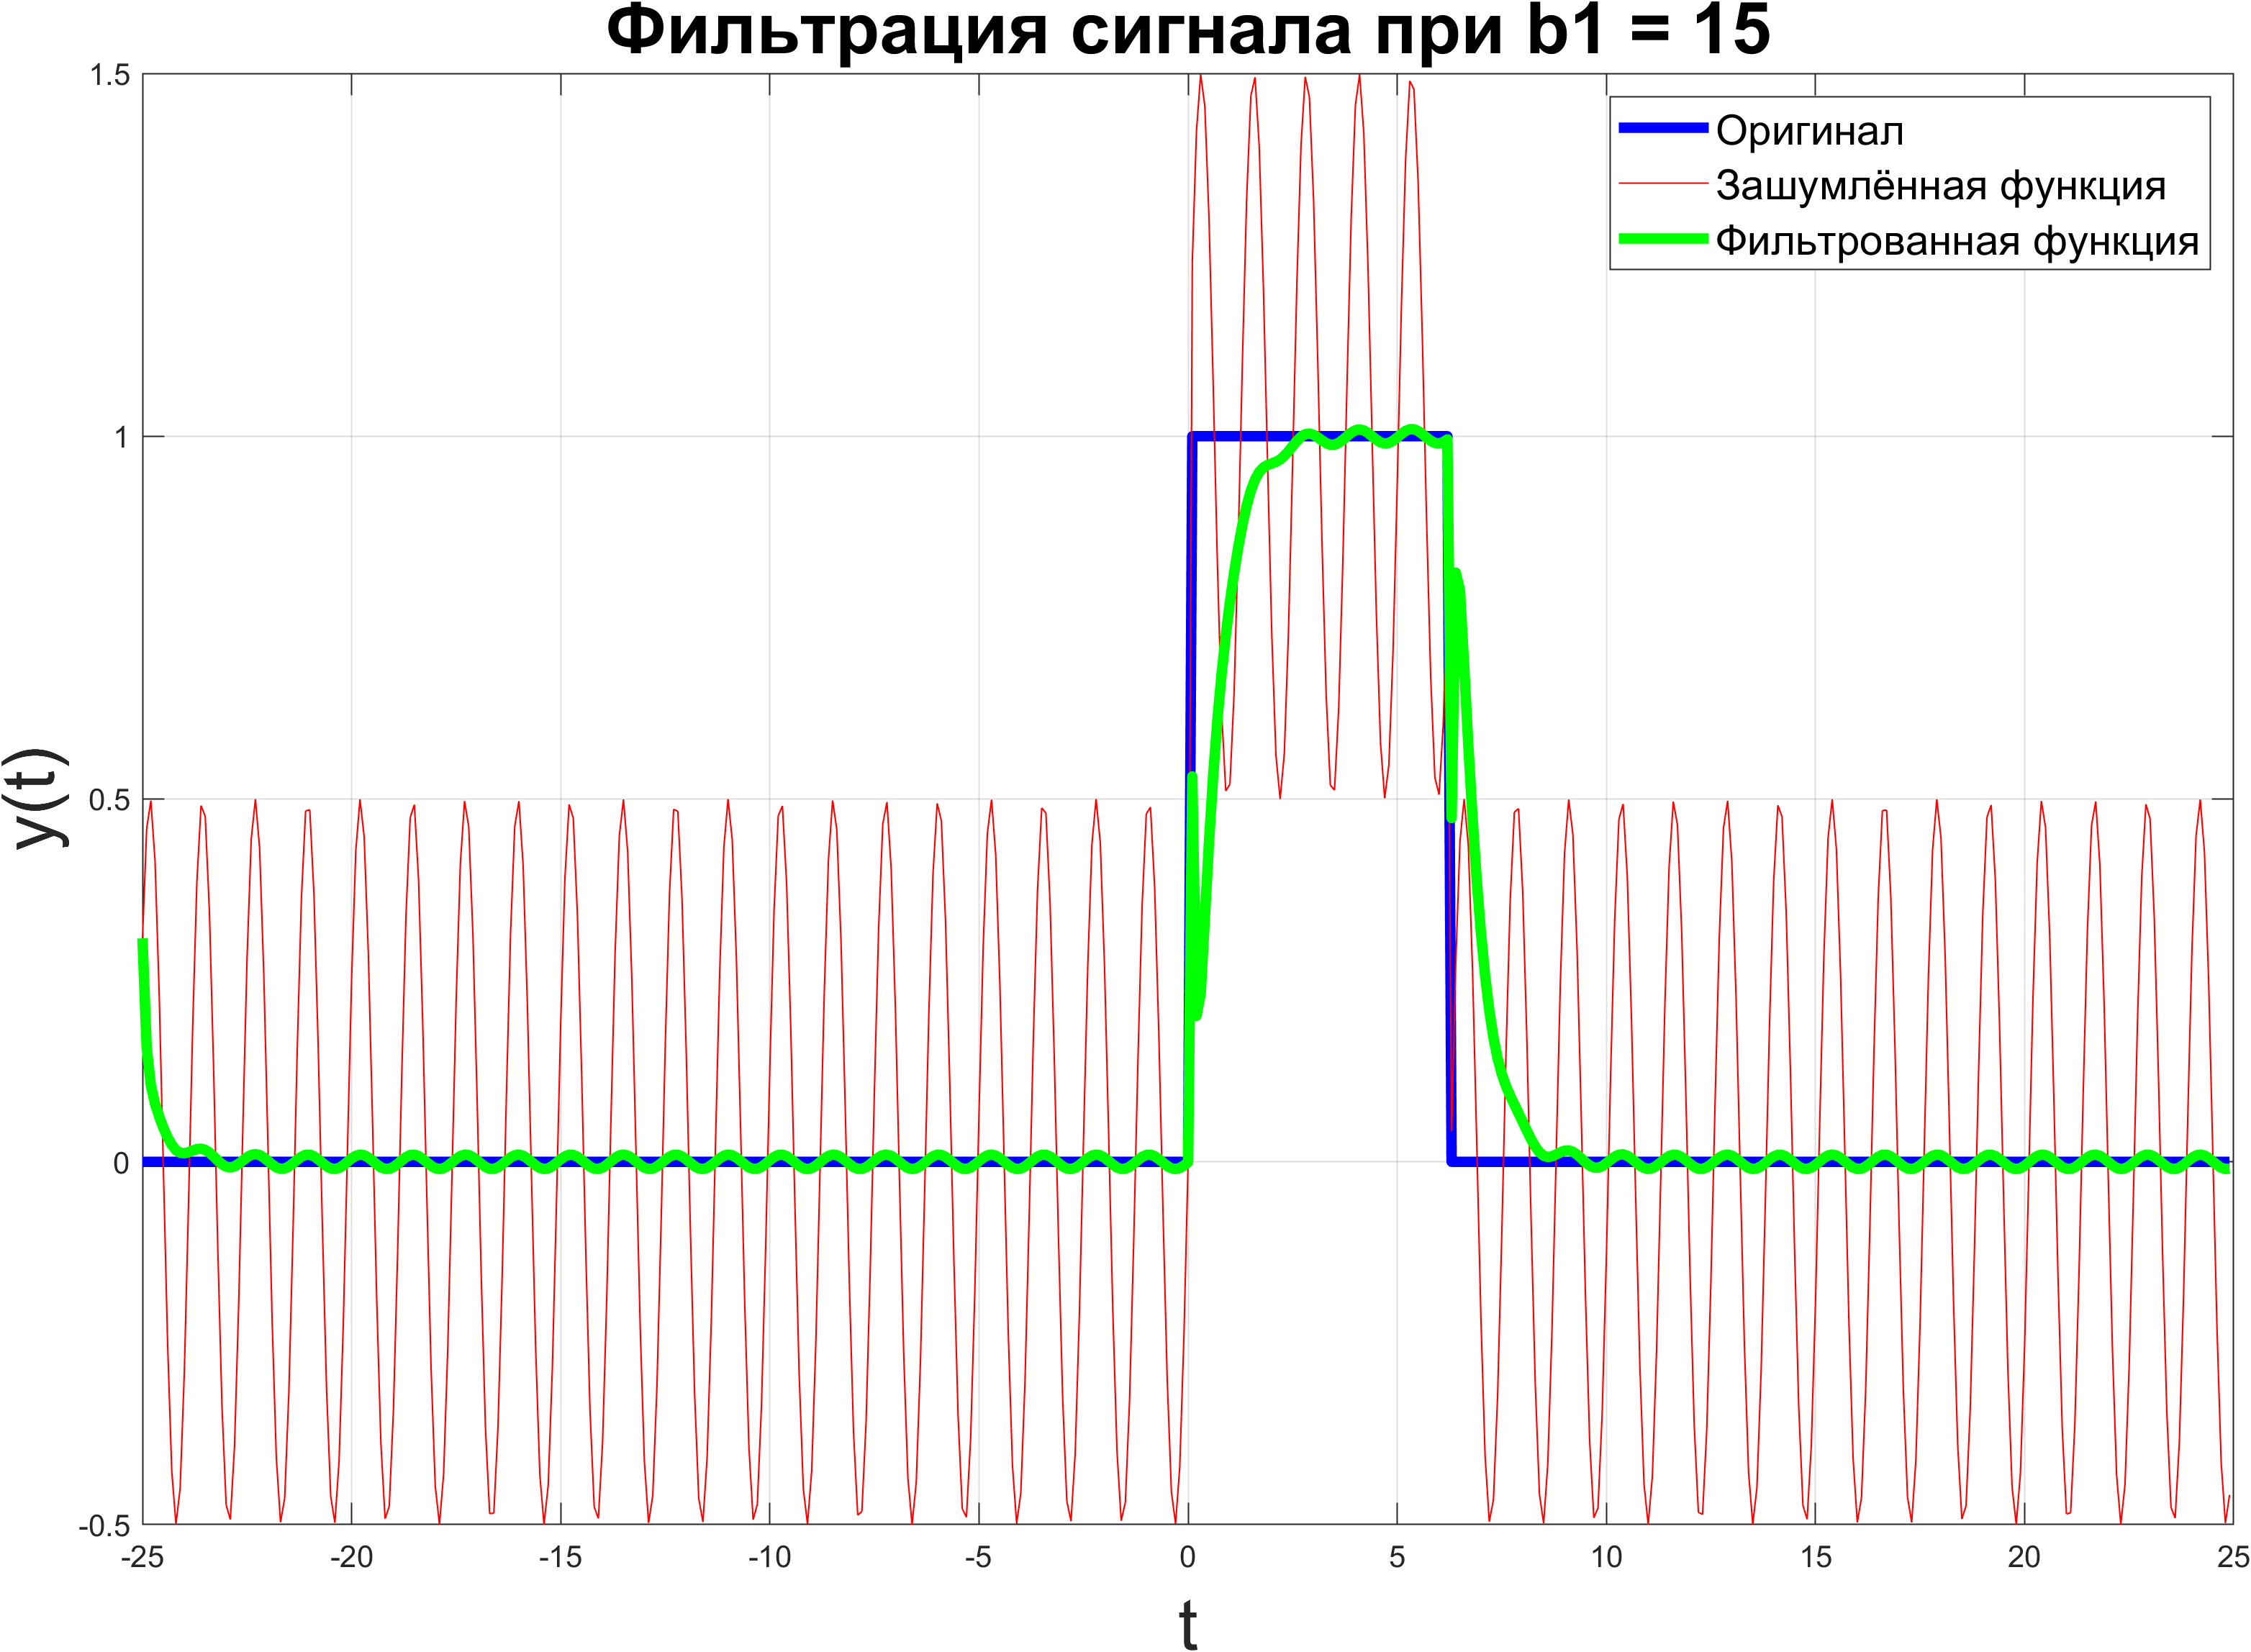
\includegraphics[width=0.92\textwidth, keepaspectratio]{images2/filter_b1_15.png}
    \caption{Фильтрация при $b_1 = 15$}
\end{figure}
\newpage
\begin{figure}[H]
    \centering
    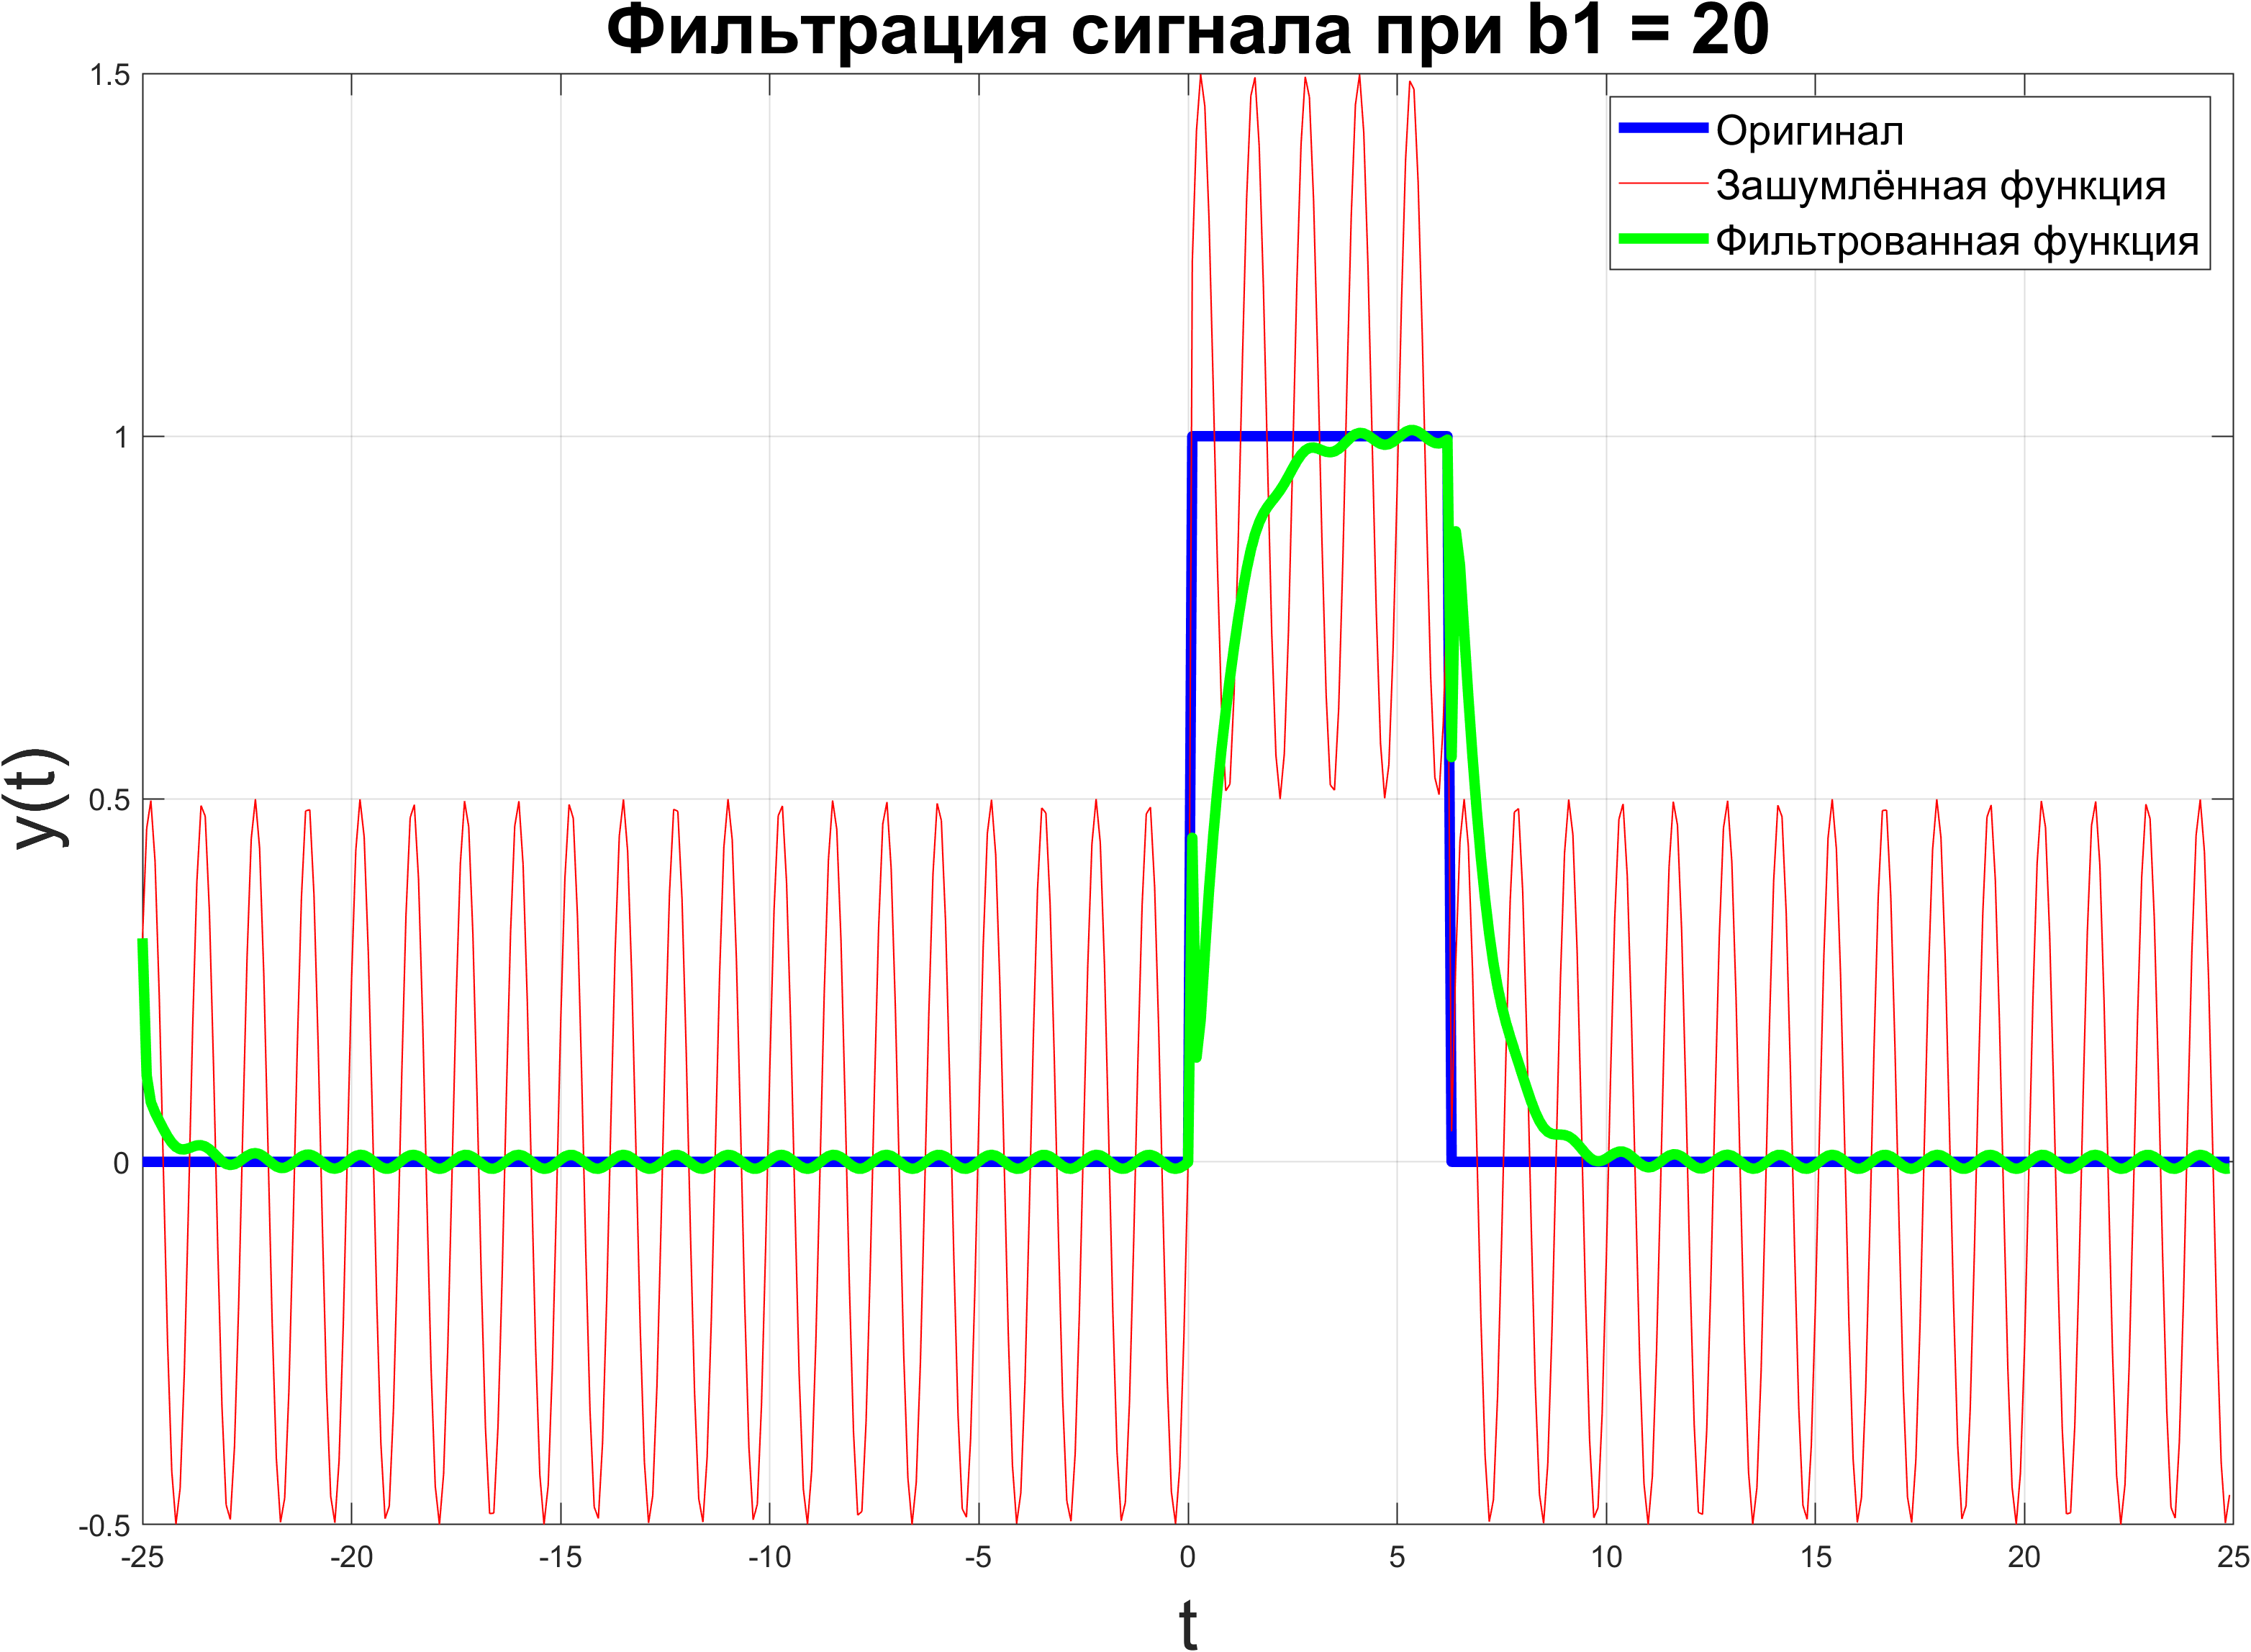
\includegraphics[width=0.92\textwidth, keepaspectratio]{images2/filter_b1_20.png}
    \caption{Фильтрация при $b_1 = 20$}
\end{figure}
\begin{figure}[H]
    \centering
    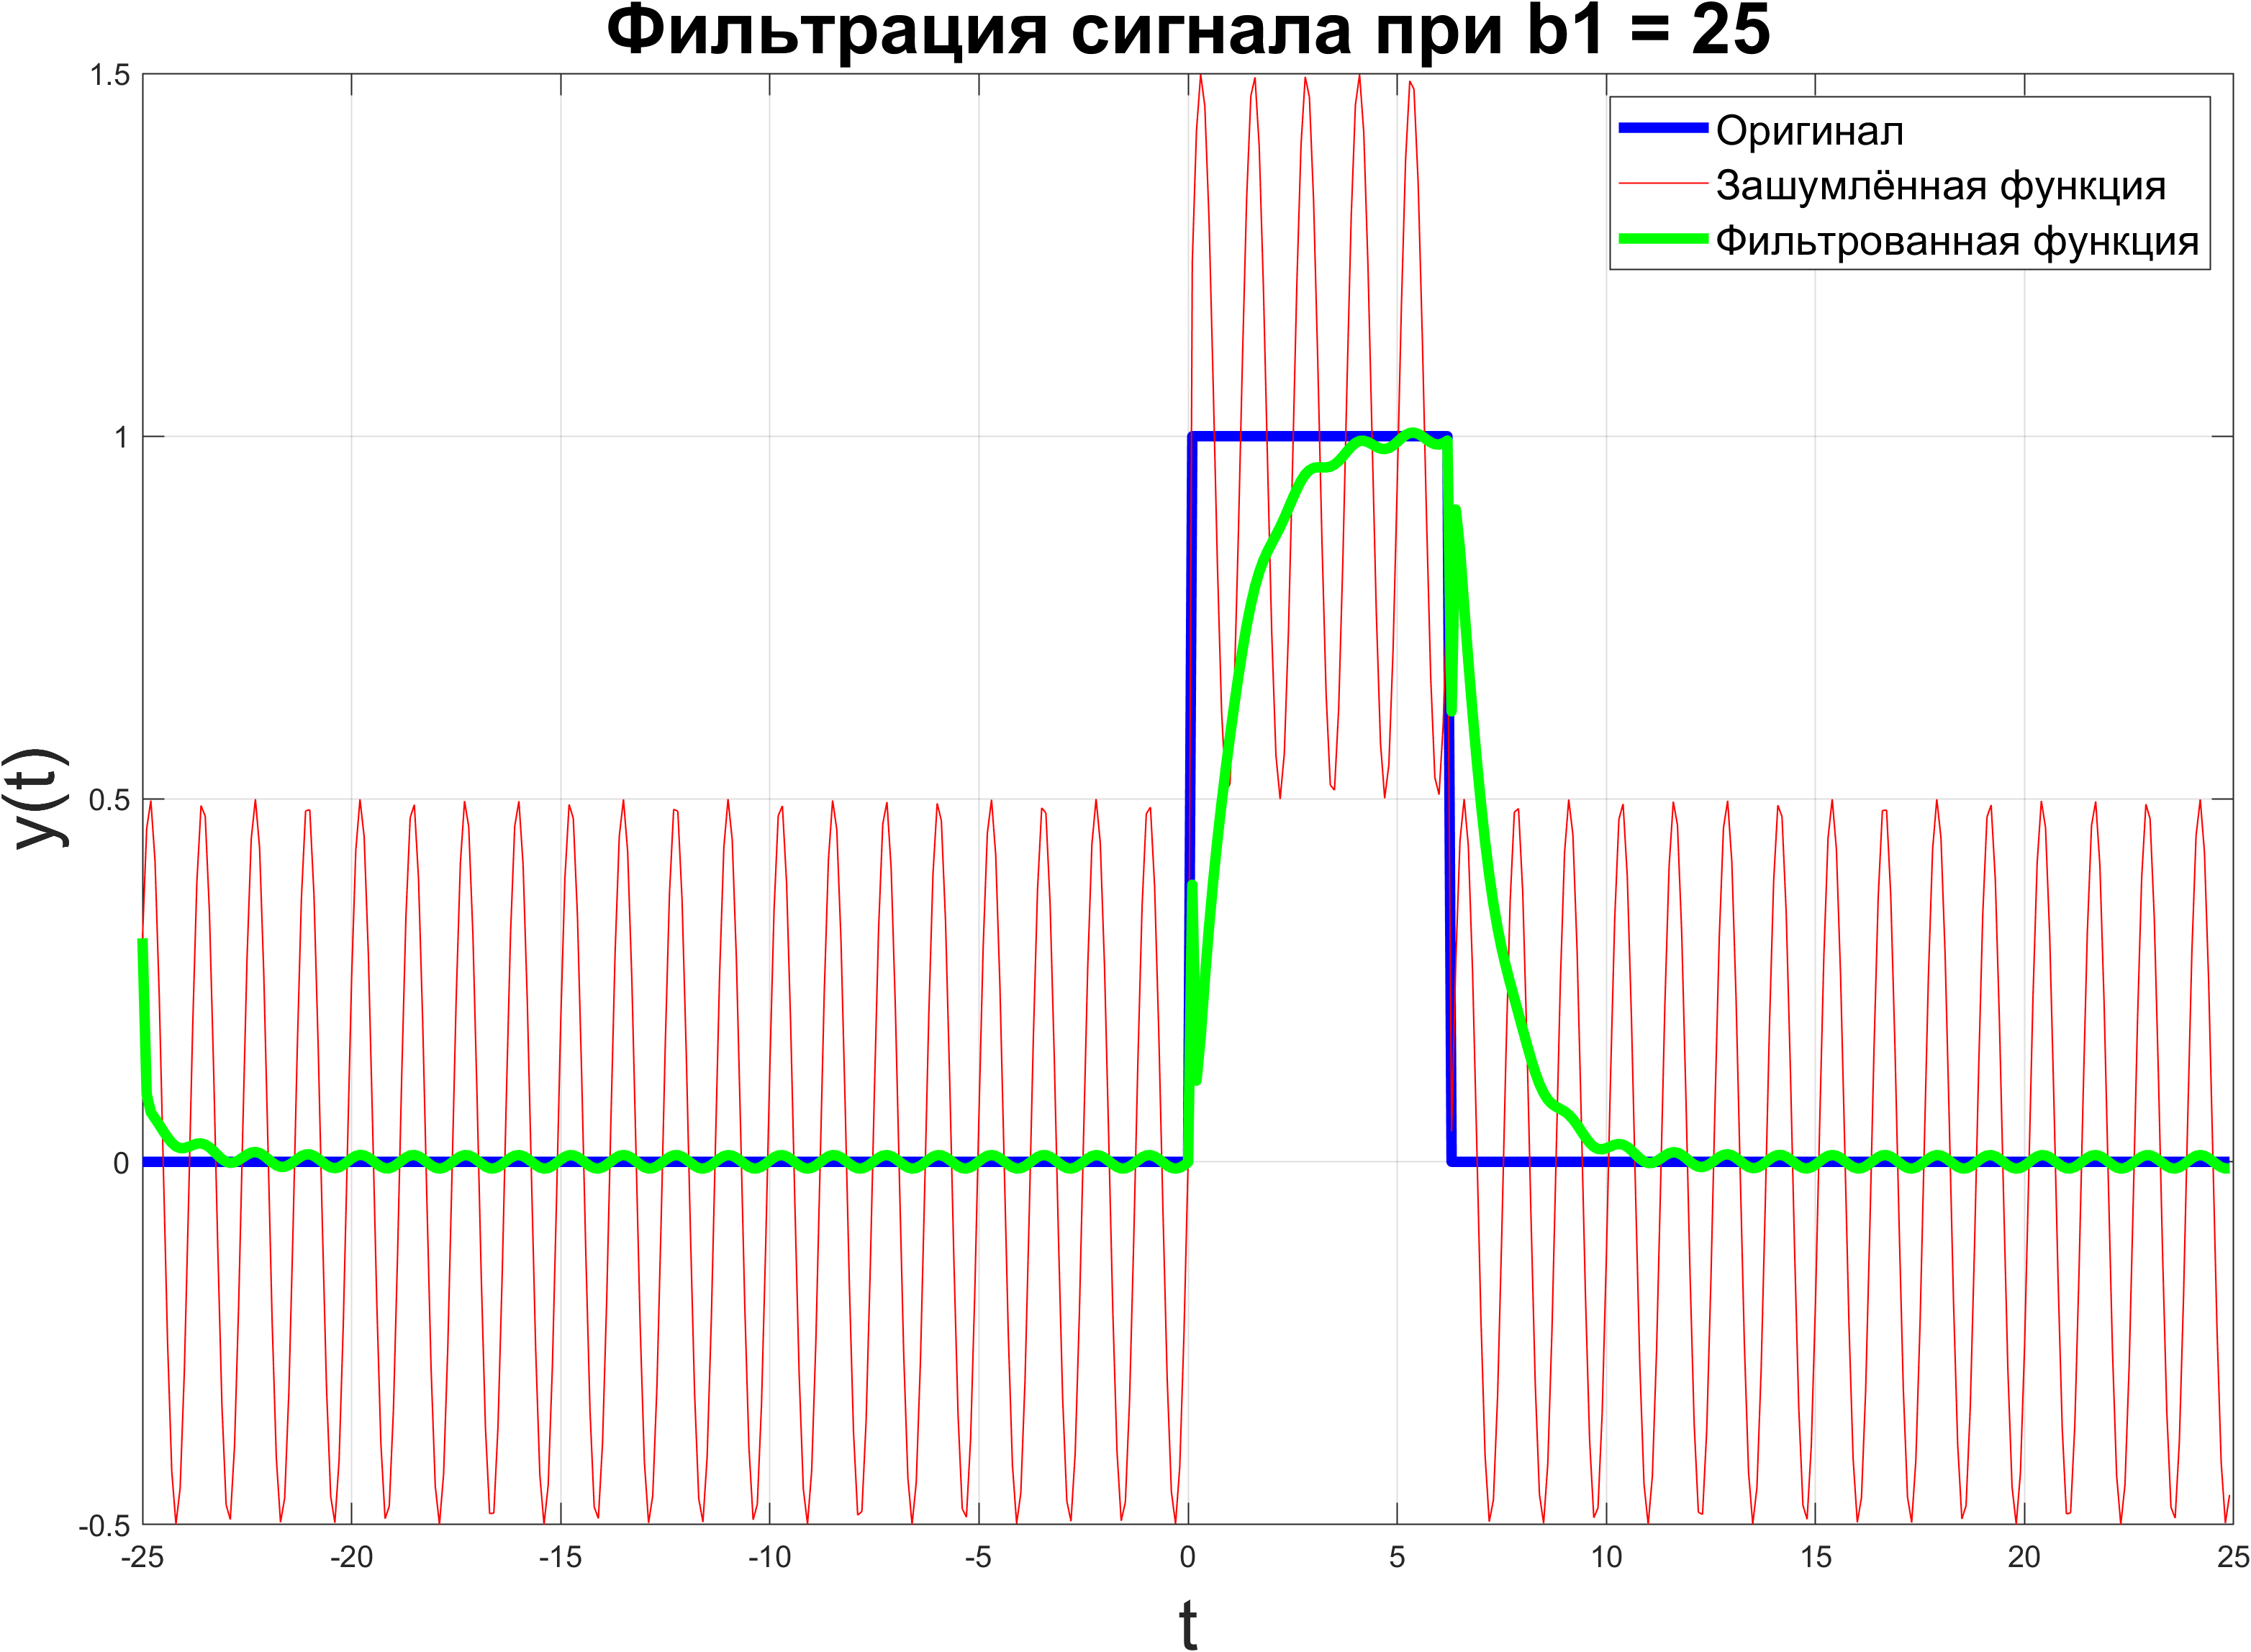
\includegraphics[width=0.92\textwidth, keepaspectratio]{images2/filter_b1_25.png}
    \caption{Фильтрация при $b_1 = 25$}
\end{figure}
\newpage

Сравнение фильтрованного сигнала и обратного Фурье-образа произведения частотной передаточной функции на Фурье-образ зашумленной функции:
\begin{figure}[H]
    \centering
    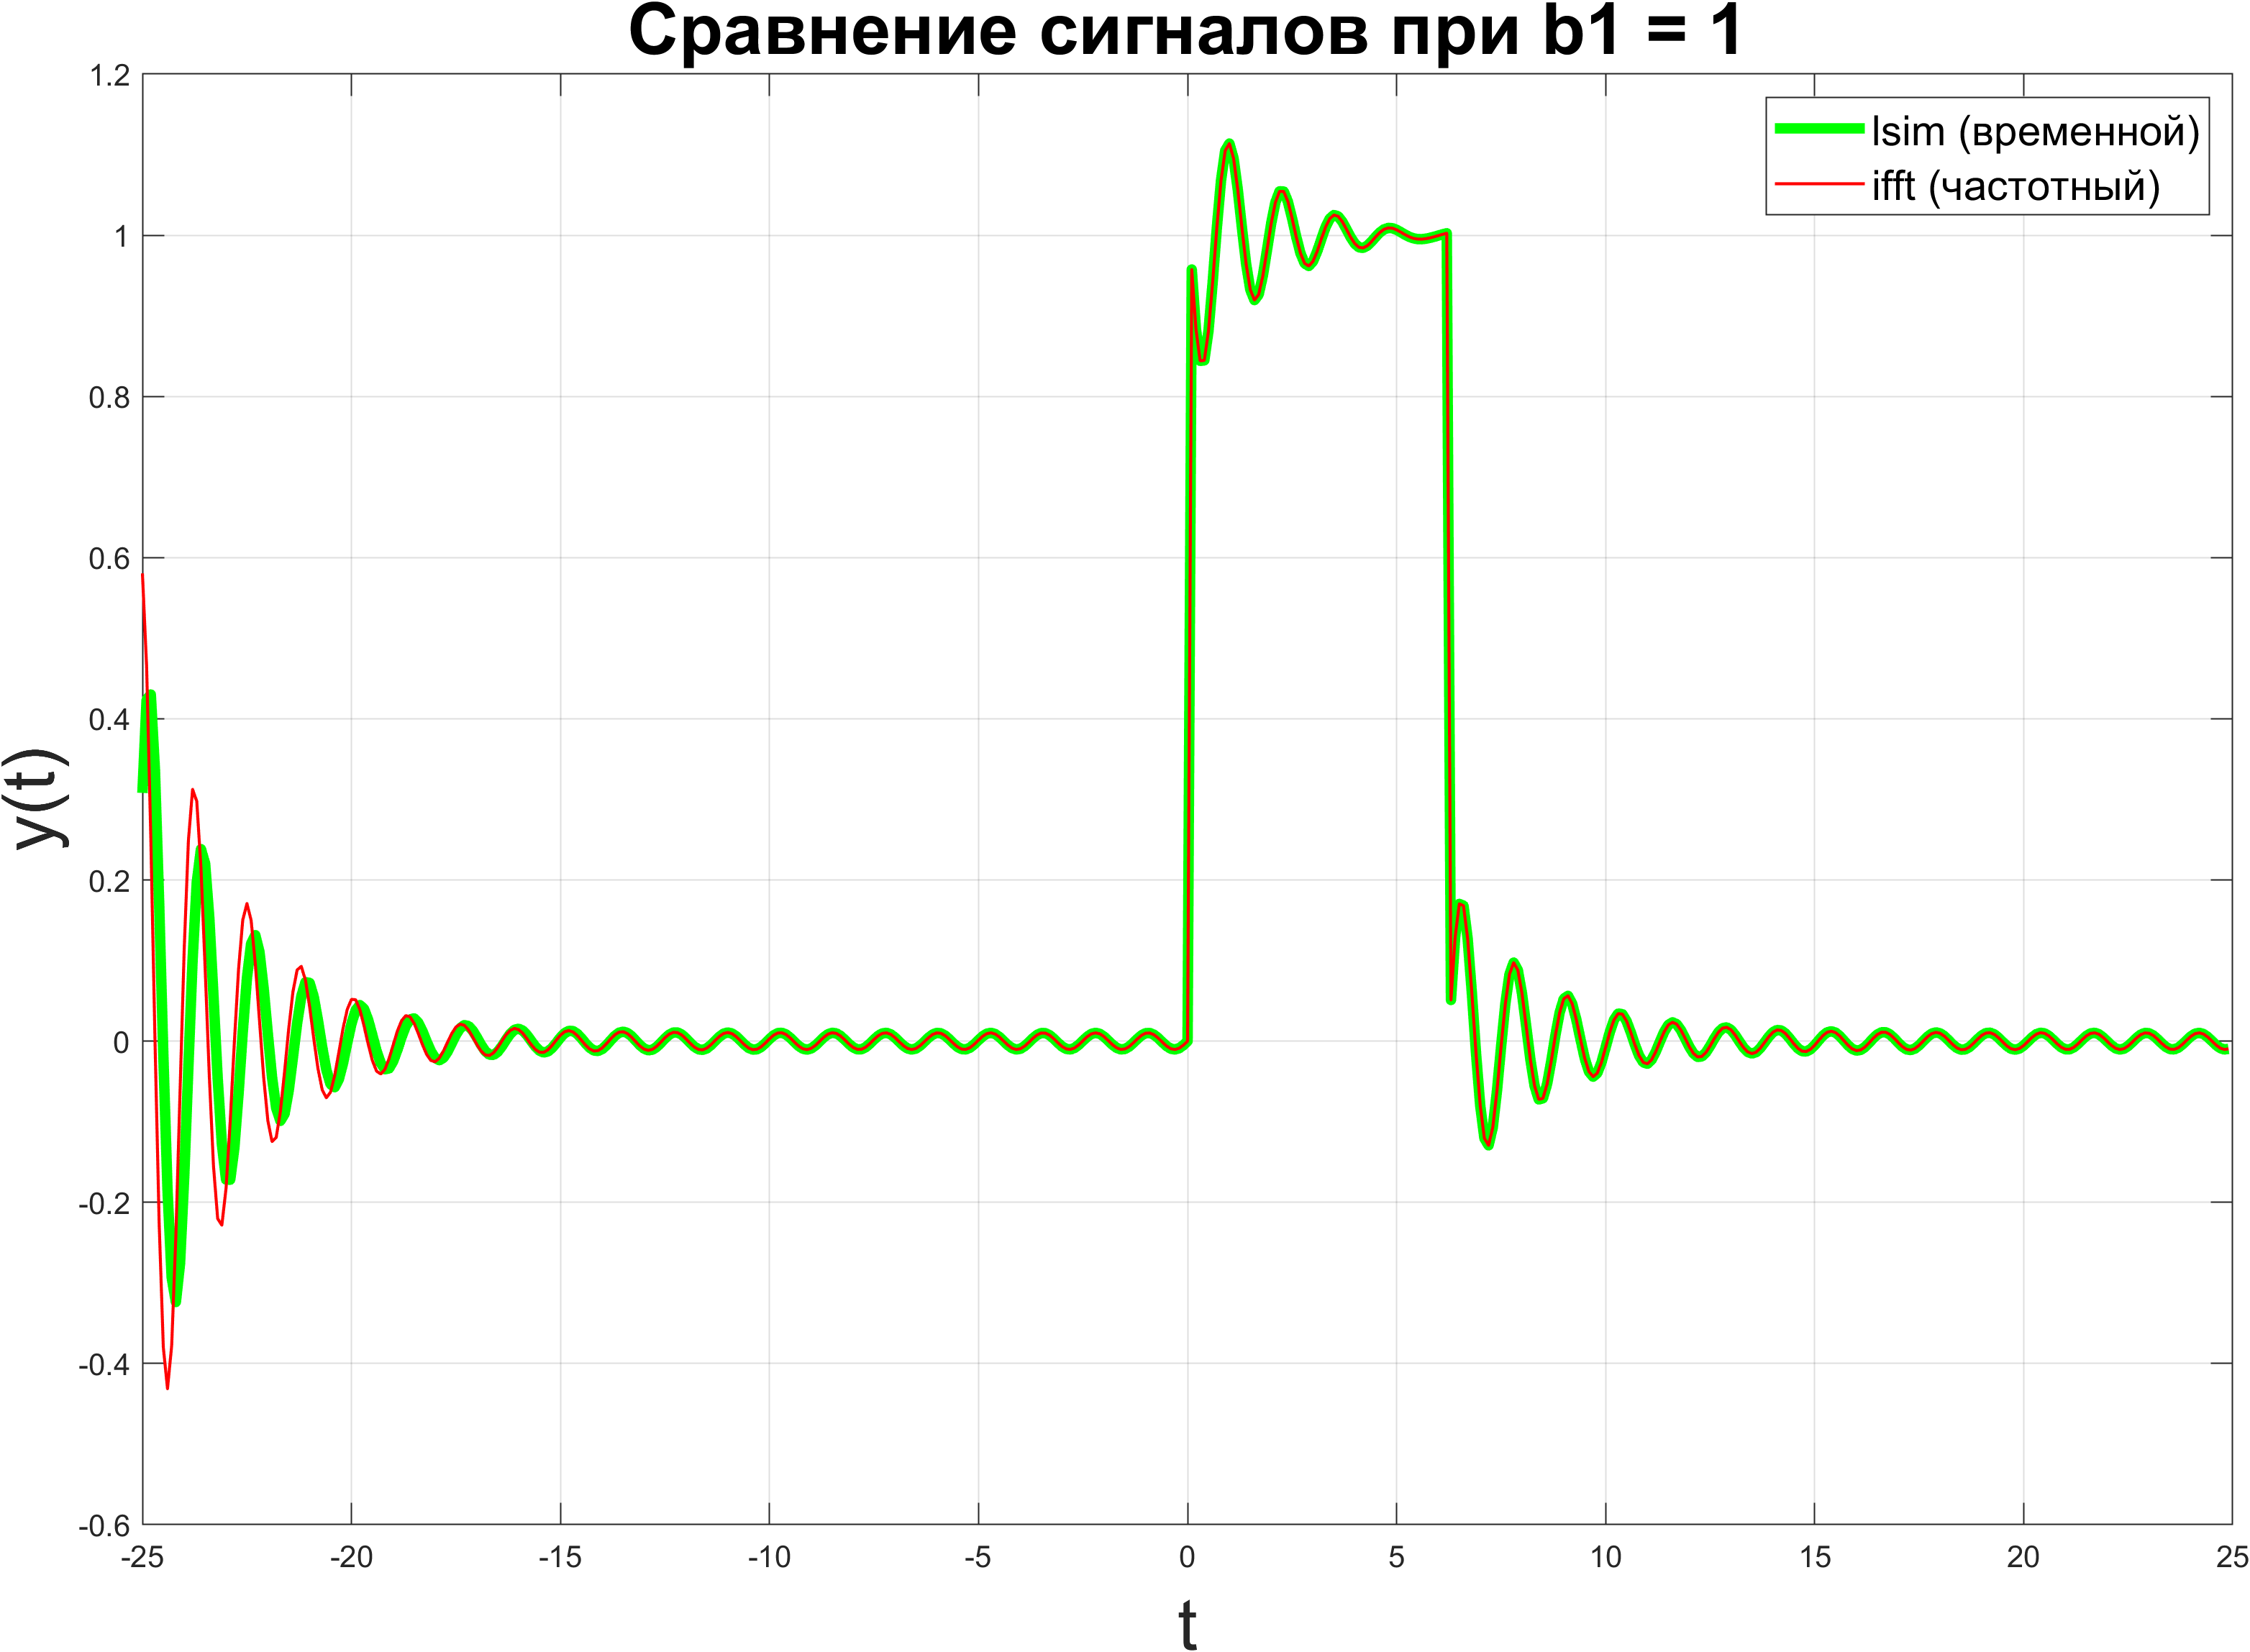
\includegraphics[width=0.85\textwidth, keepaspectratio]{images2/filter_transf_b1_1.png}
    \caption{Сравнение методов при $b_1 = 1$}
\end{figure}
\begin{figure}[H]
    \centering
    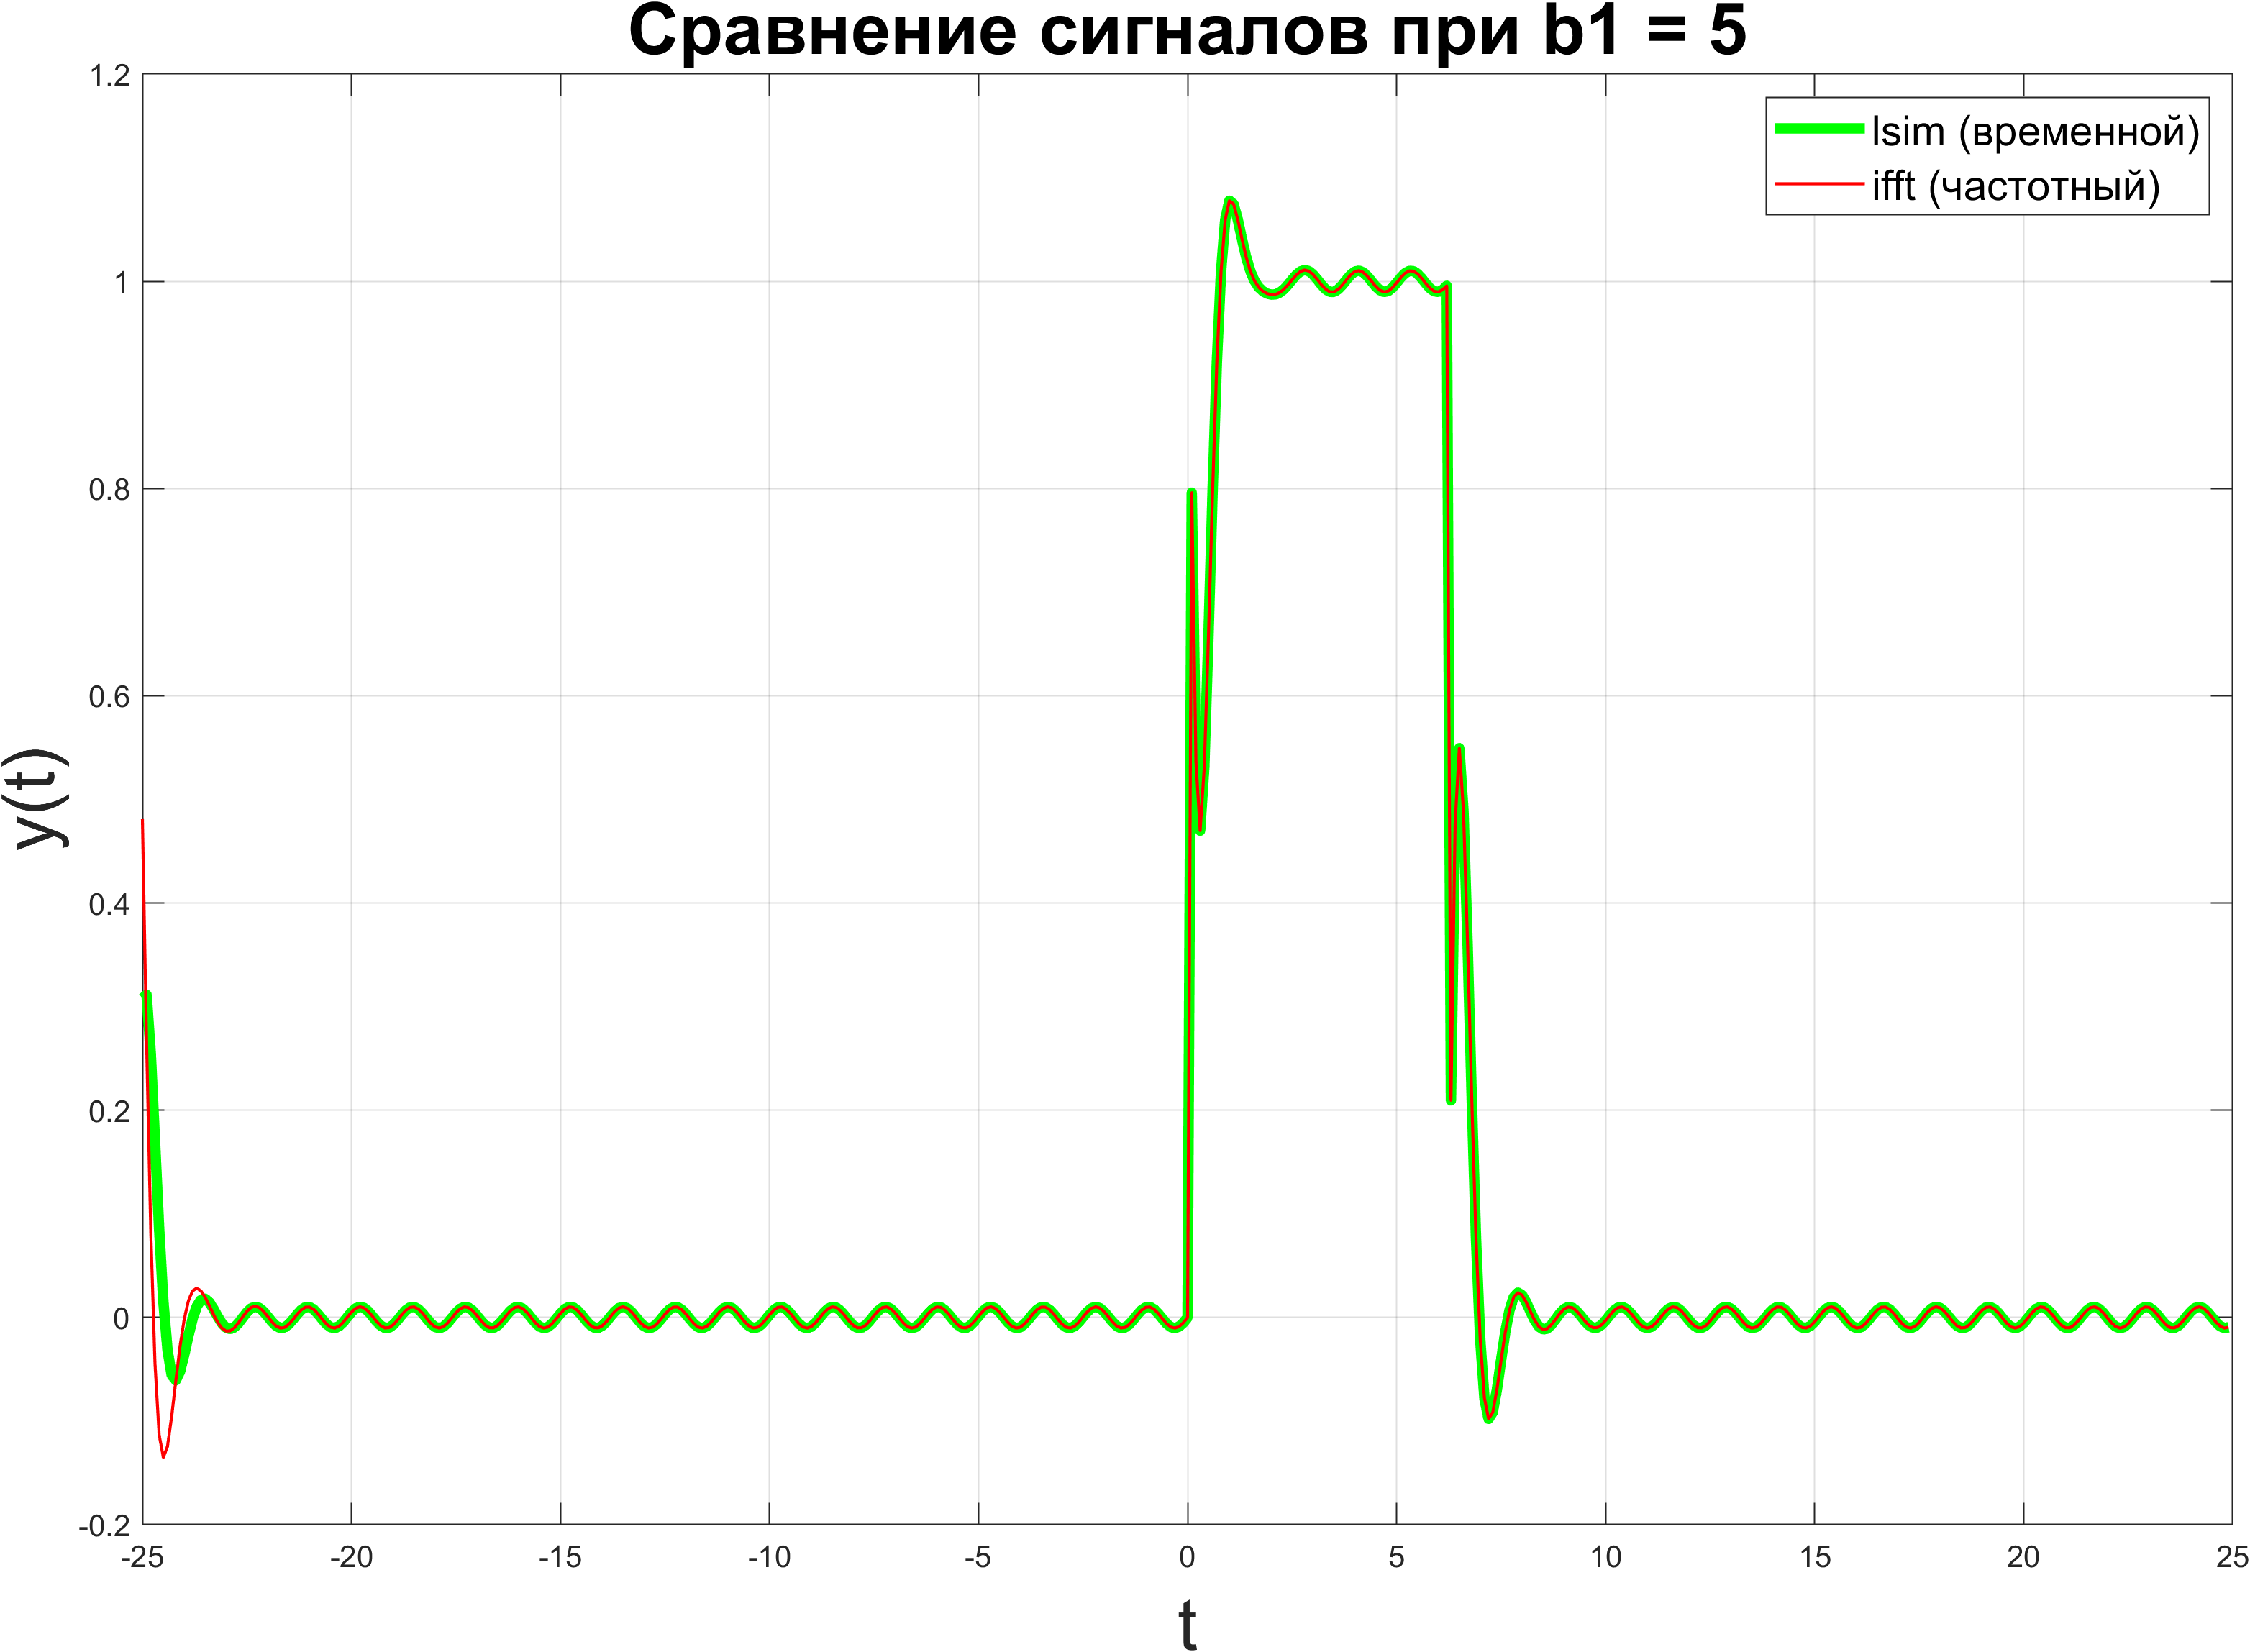
\includegraphics[width=0.85\textwidth, keepaspectratio]{images2/filter_transf_b1_5.png}
    \caption{Сравнение методов при $b_1 = 5$}
\end{figure}
\newpage
\begin{figure}[H]
    \centering
    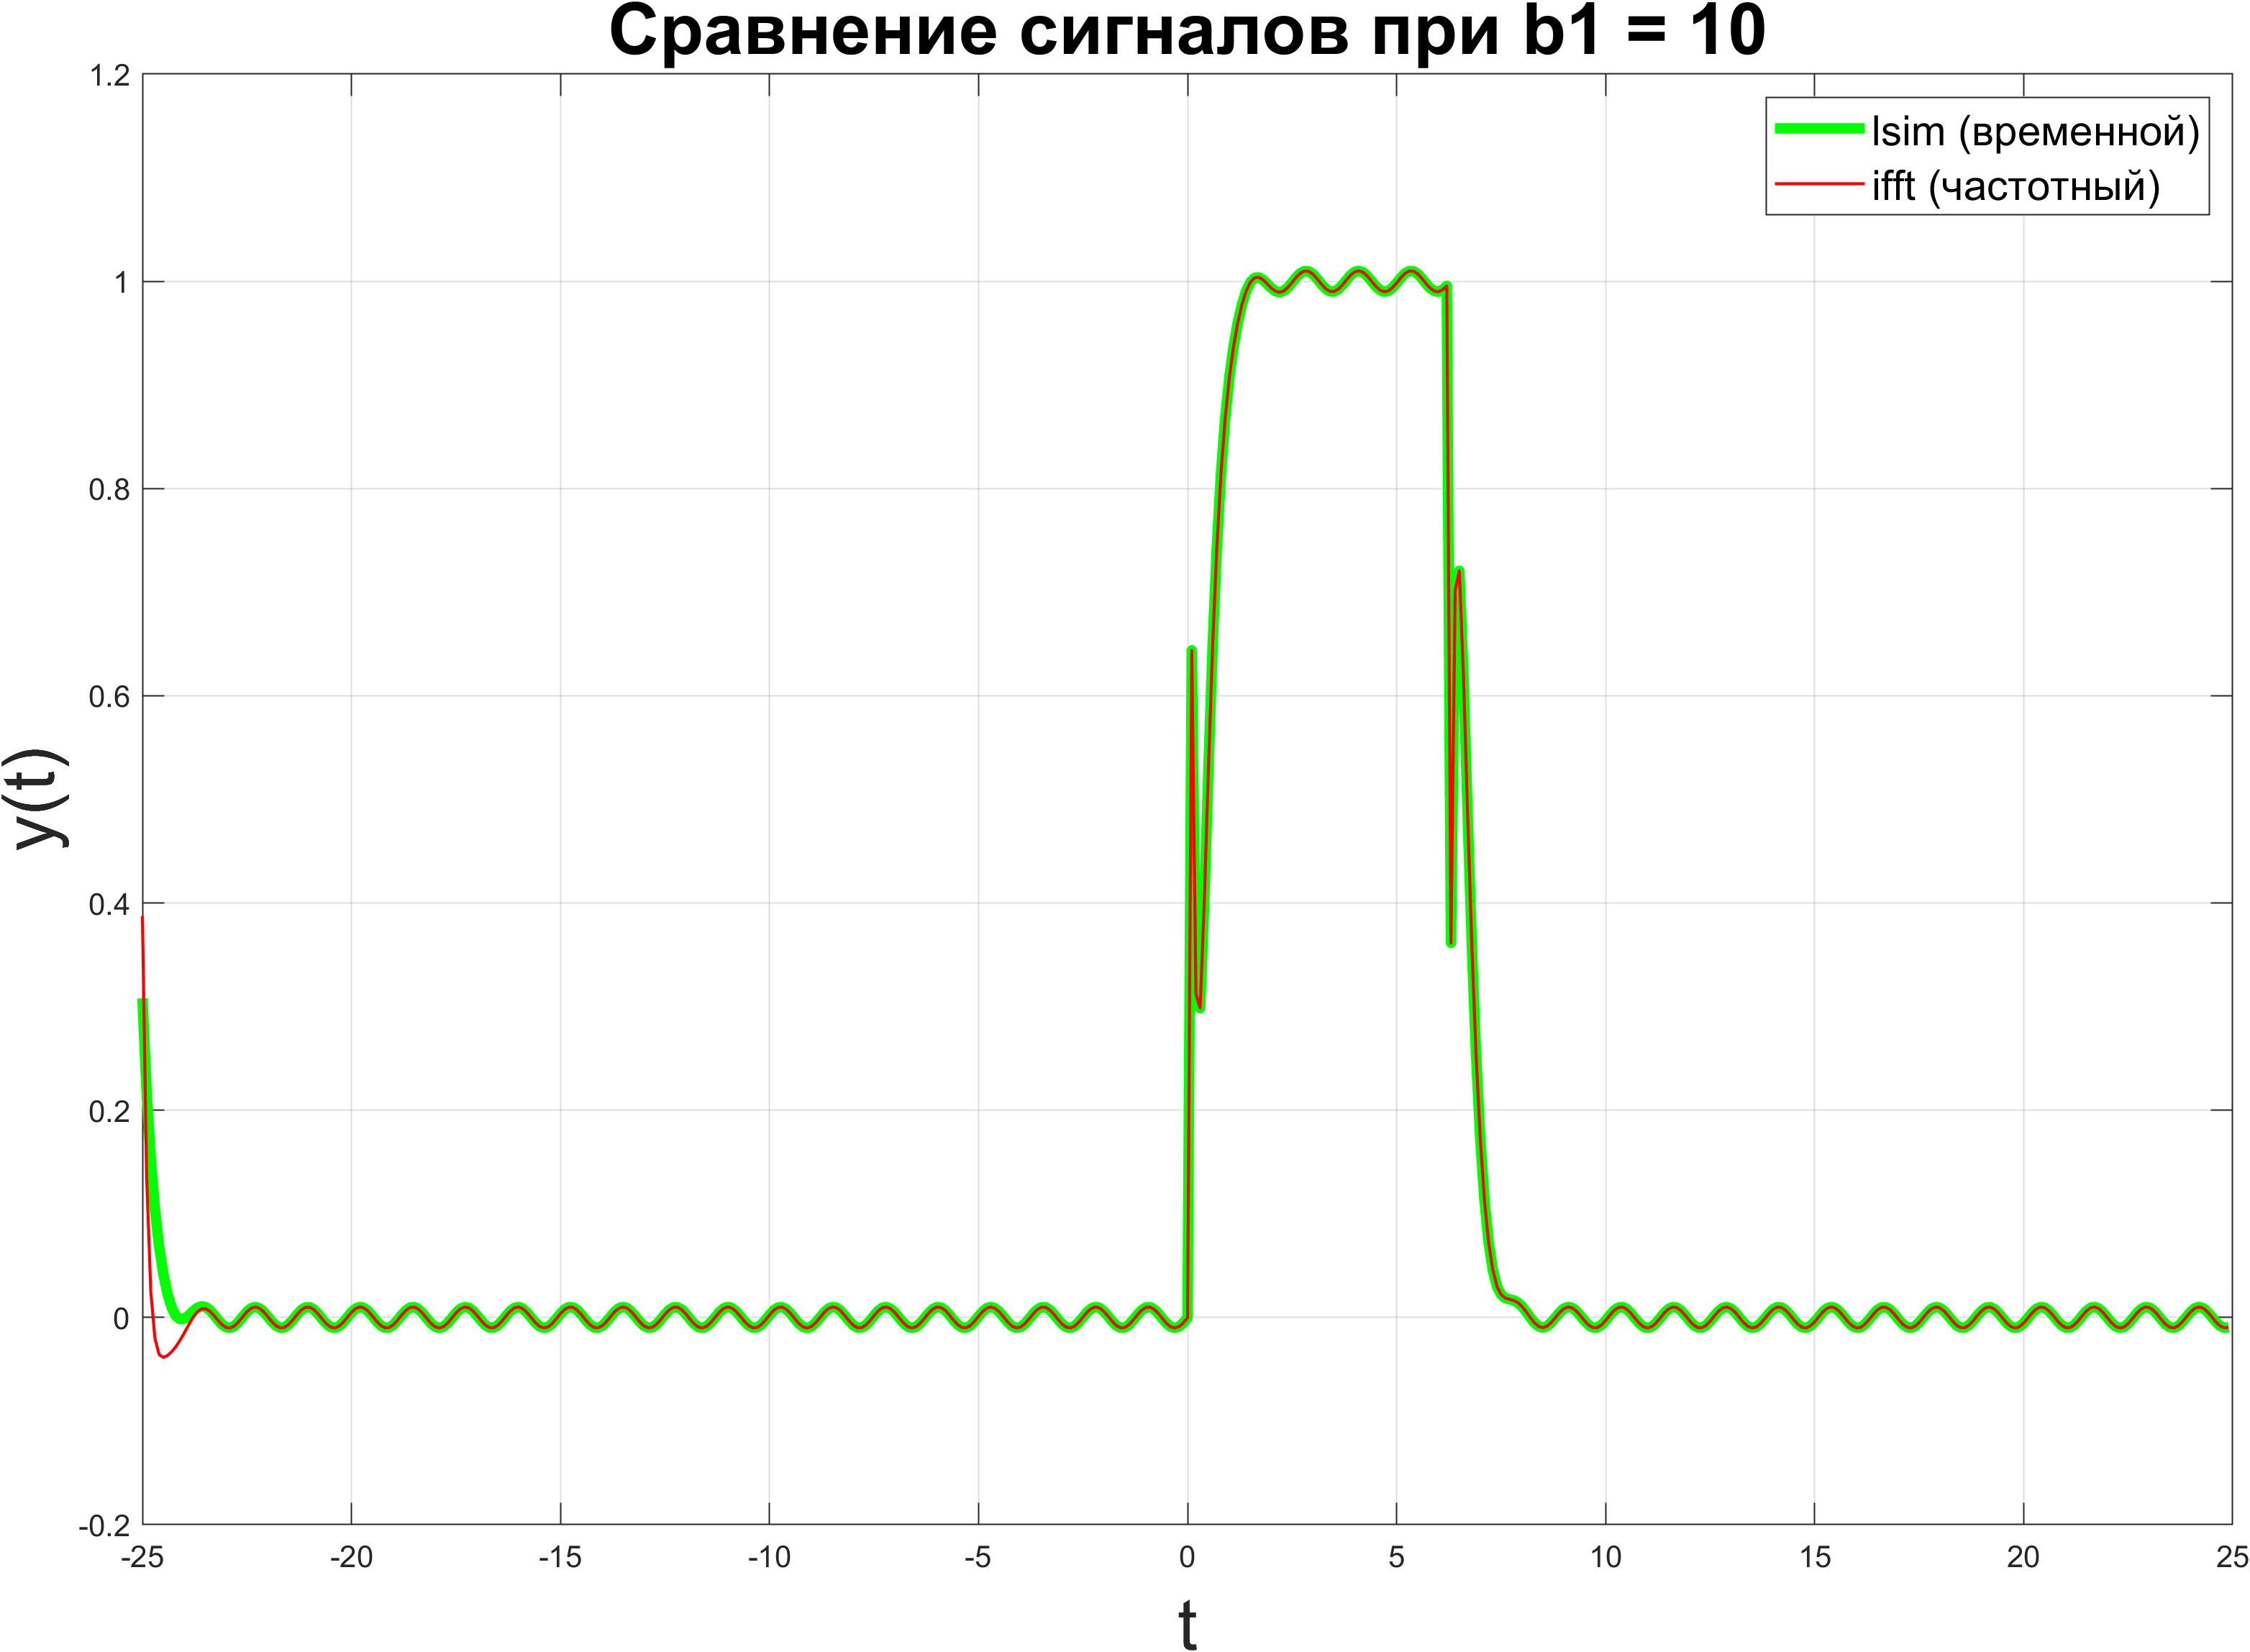
\includegraphics[width=0.92\textwidth, keepaspectratio]{images2/filter_transf_b1_10.png}
    \caption{Сравнение методов при $b_1 = 10$}
\end{figure}
\begin{figure}[H]
    \centering
    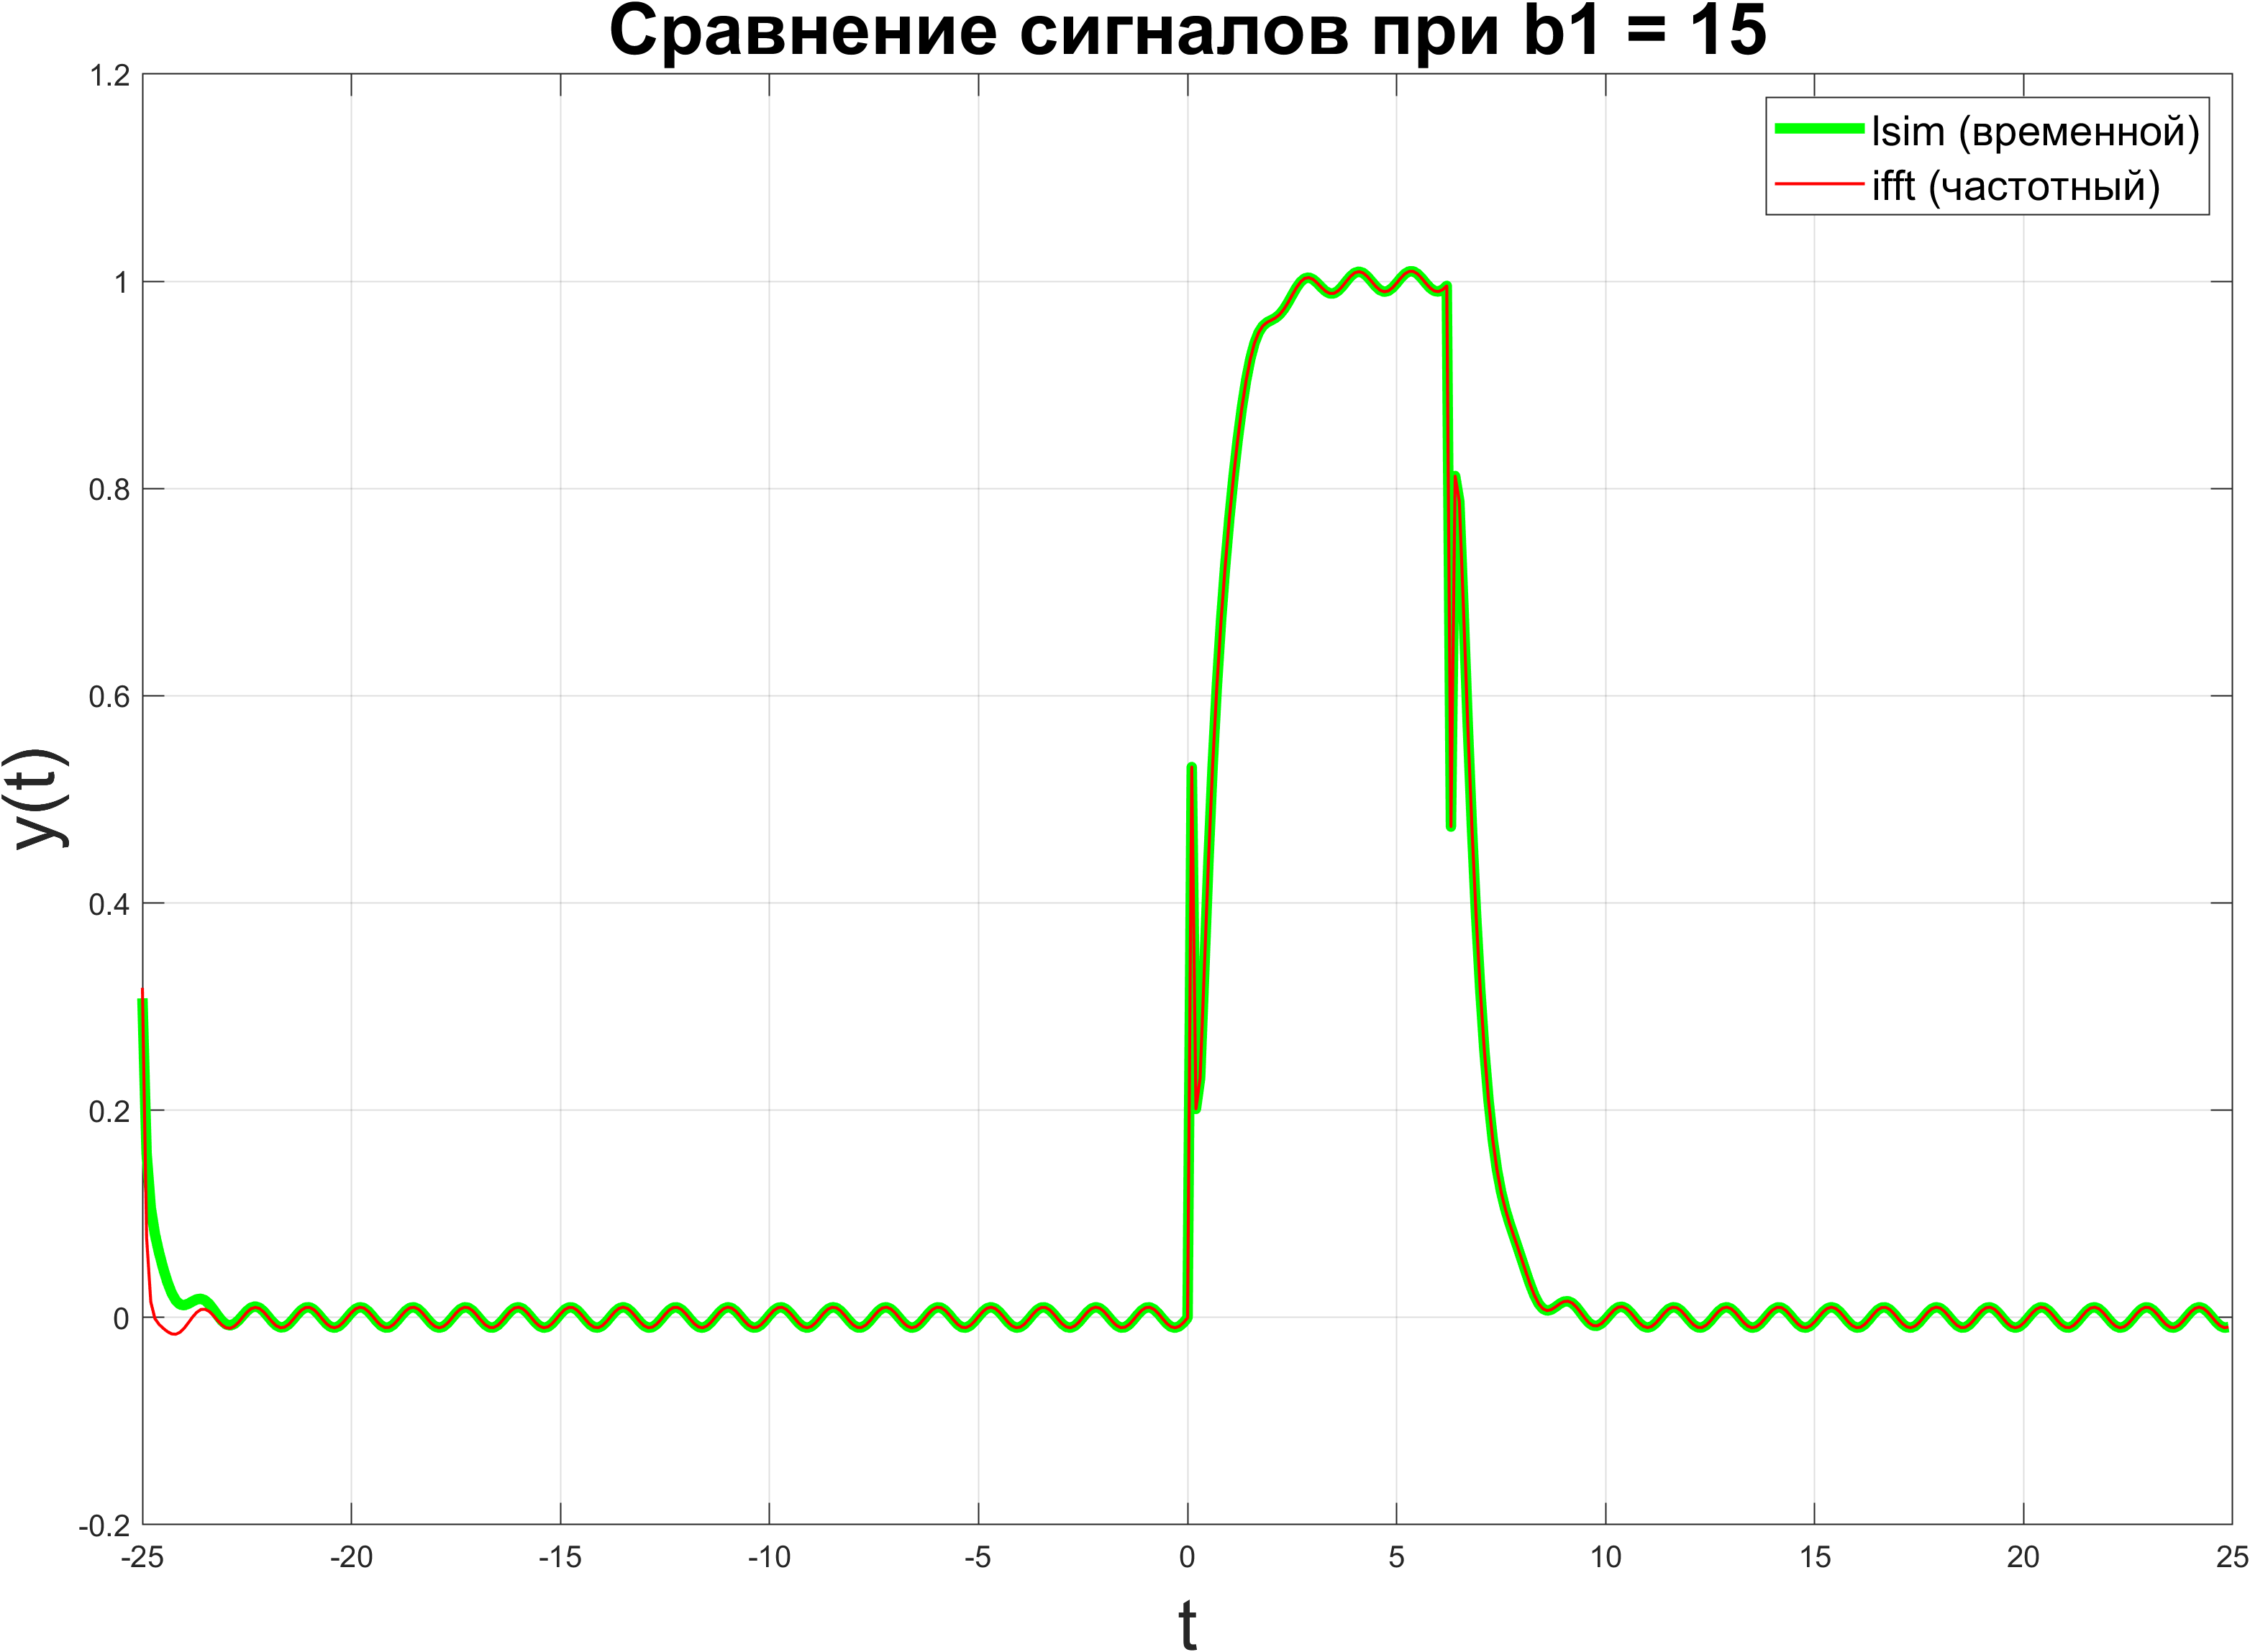
\includegraphics[width=0.92\textwidth, keepaspectratio]{images2/filter_transf_b1_15.png}
    \caption{Сравнение методов при $b_1 = 15$}
\end{figure}
\newpage
\begin{figure}[H]
    \centering
    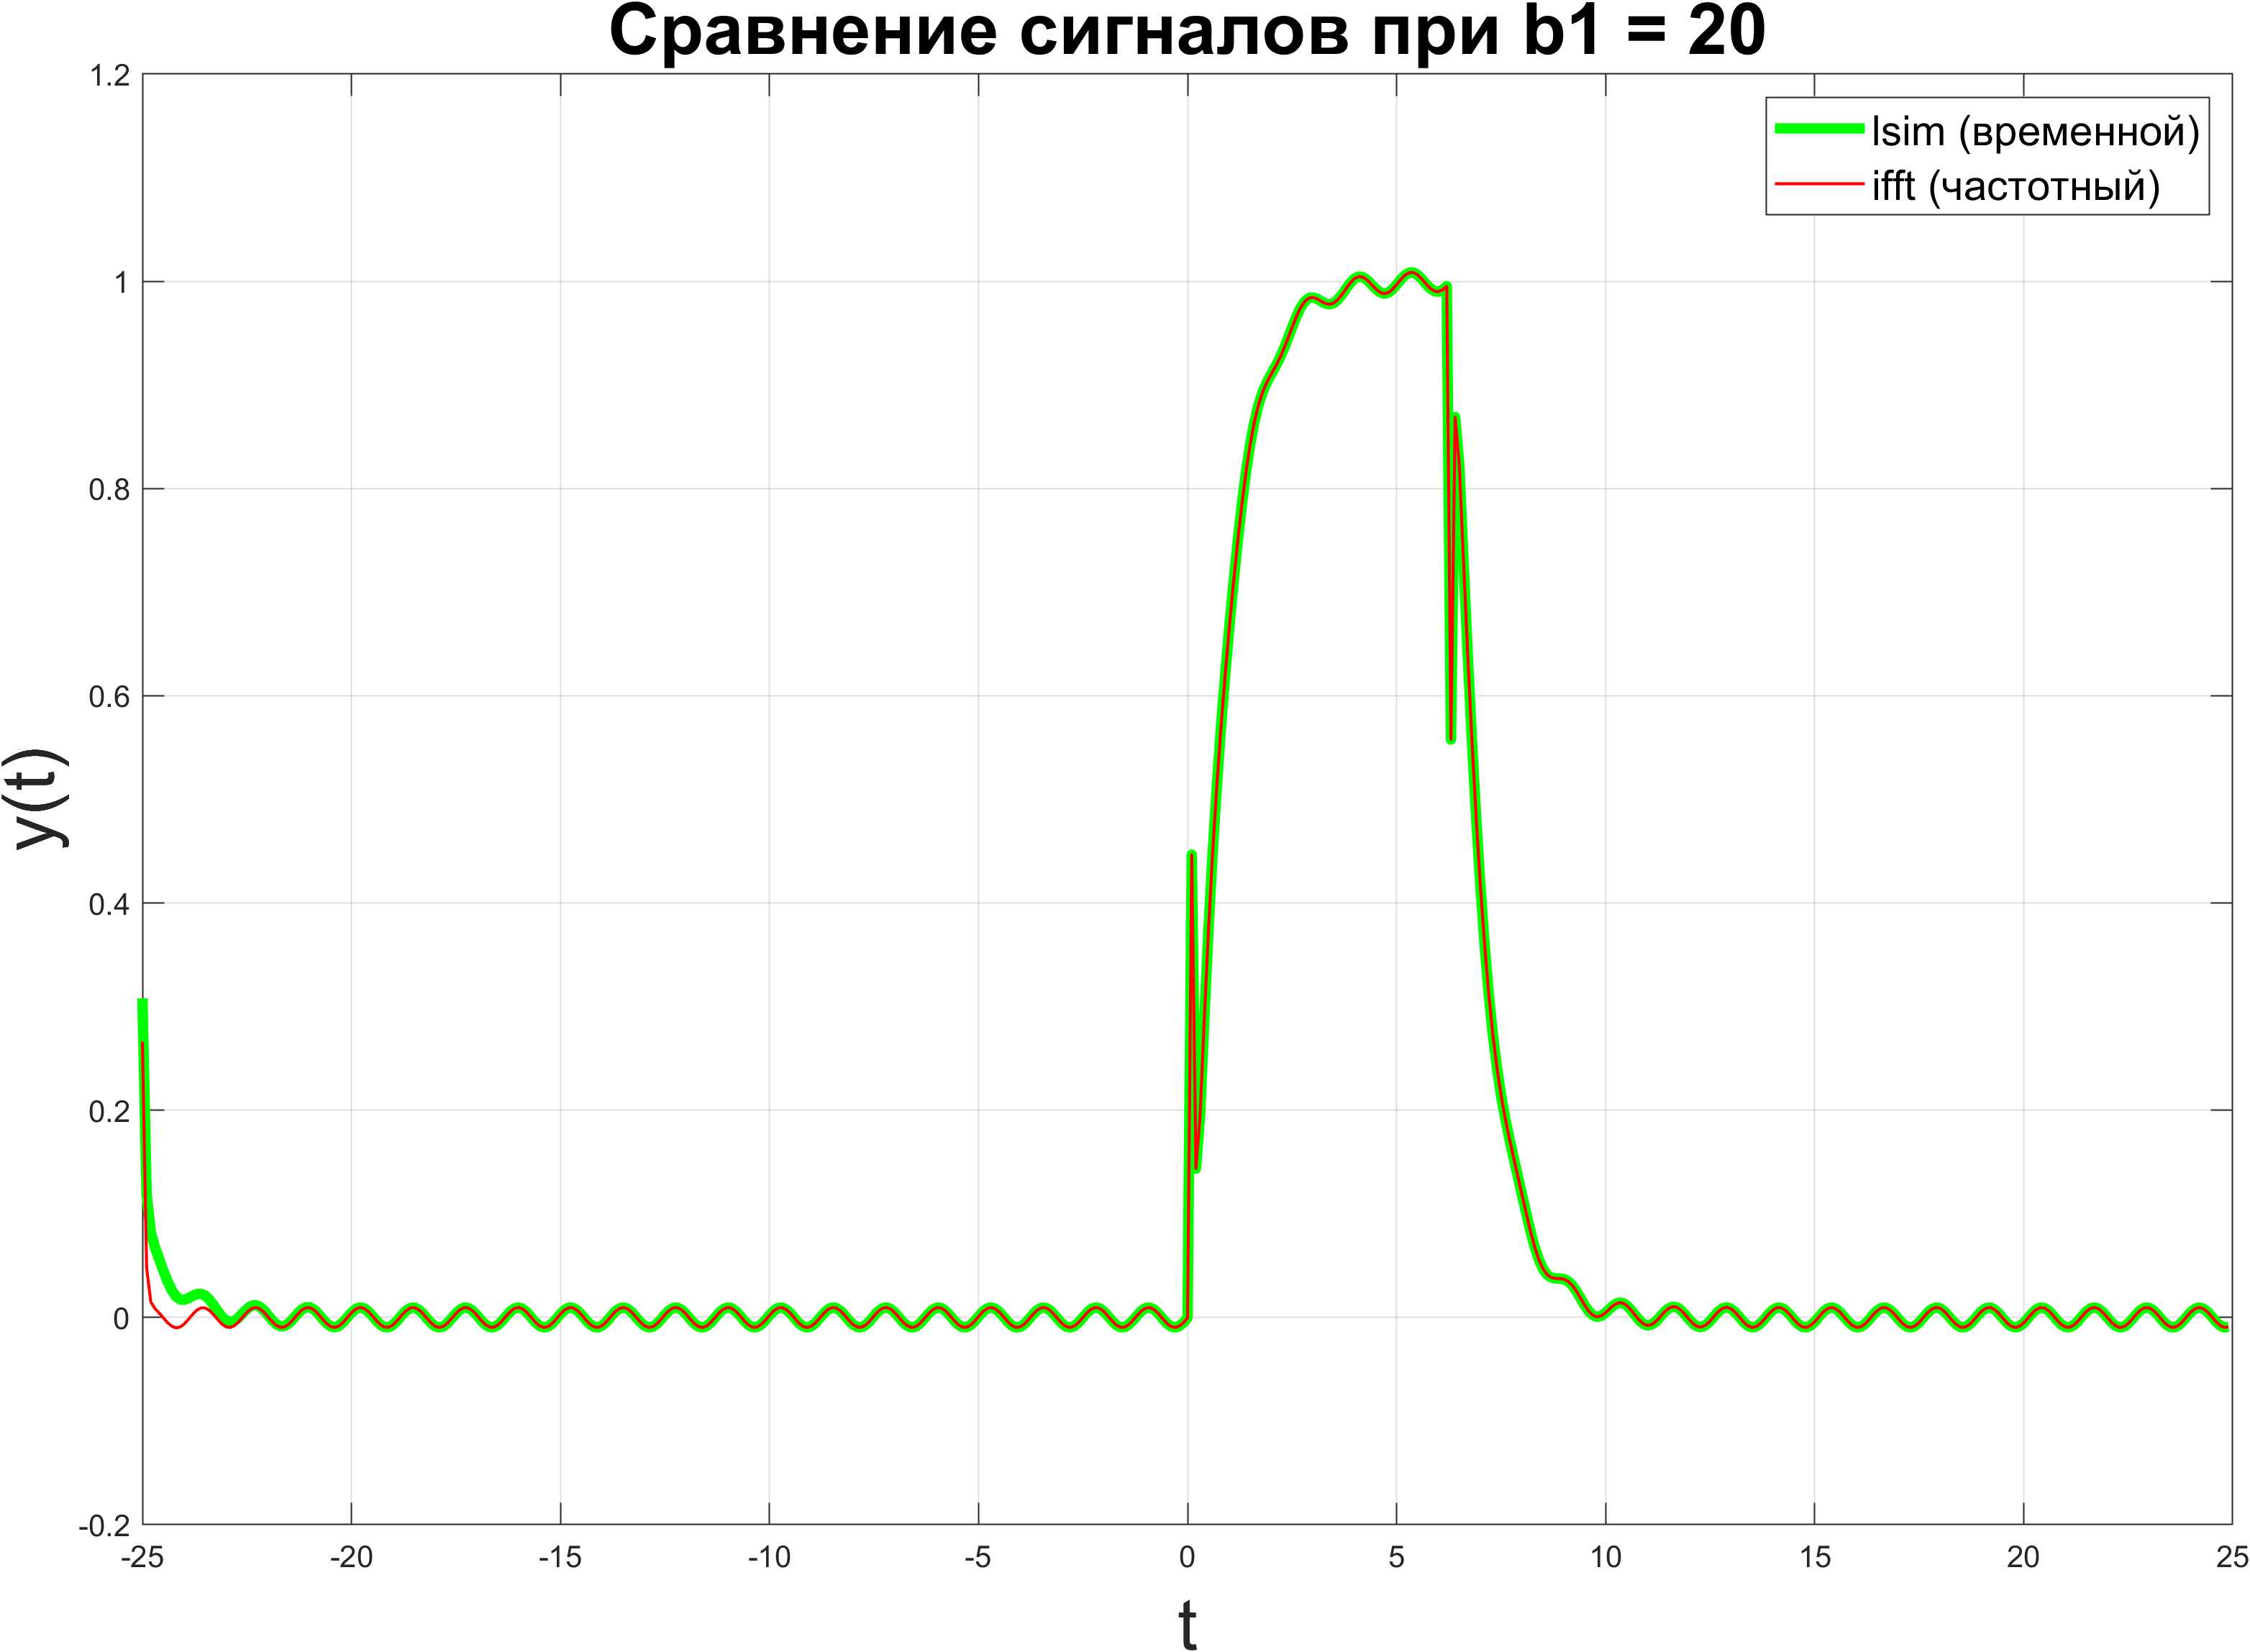
\includegraphics[width=0.92\textwidth, keepaspectratio]{images2/filter_transf_b1_20.png}
    \caption{Сравнение методов при $b_1 = 20$}
\end{figure}
\begin{figure}[H]
    \centering
    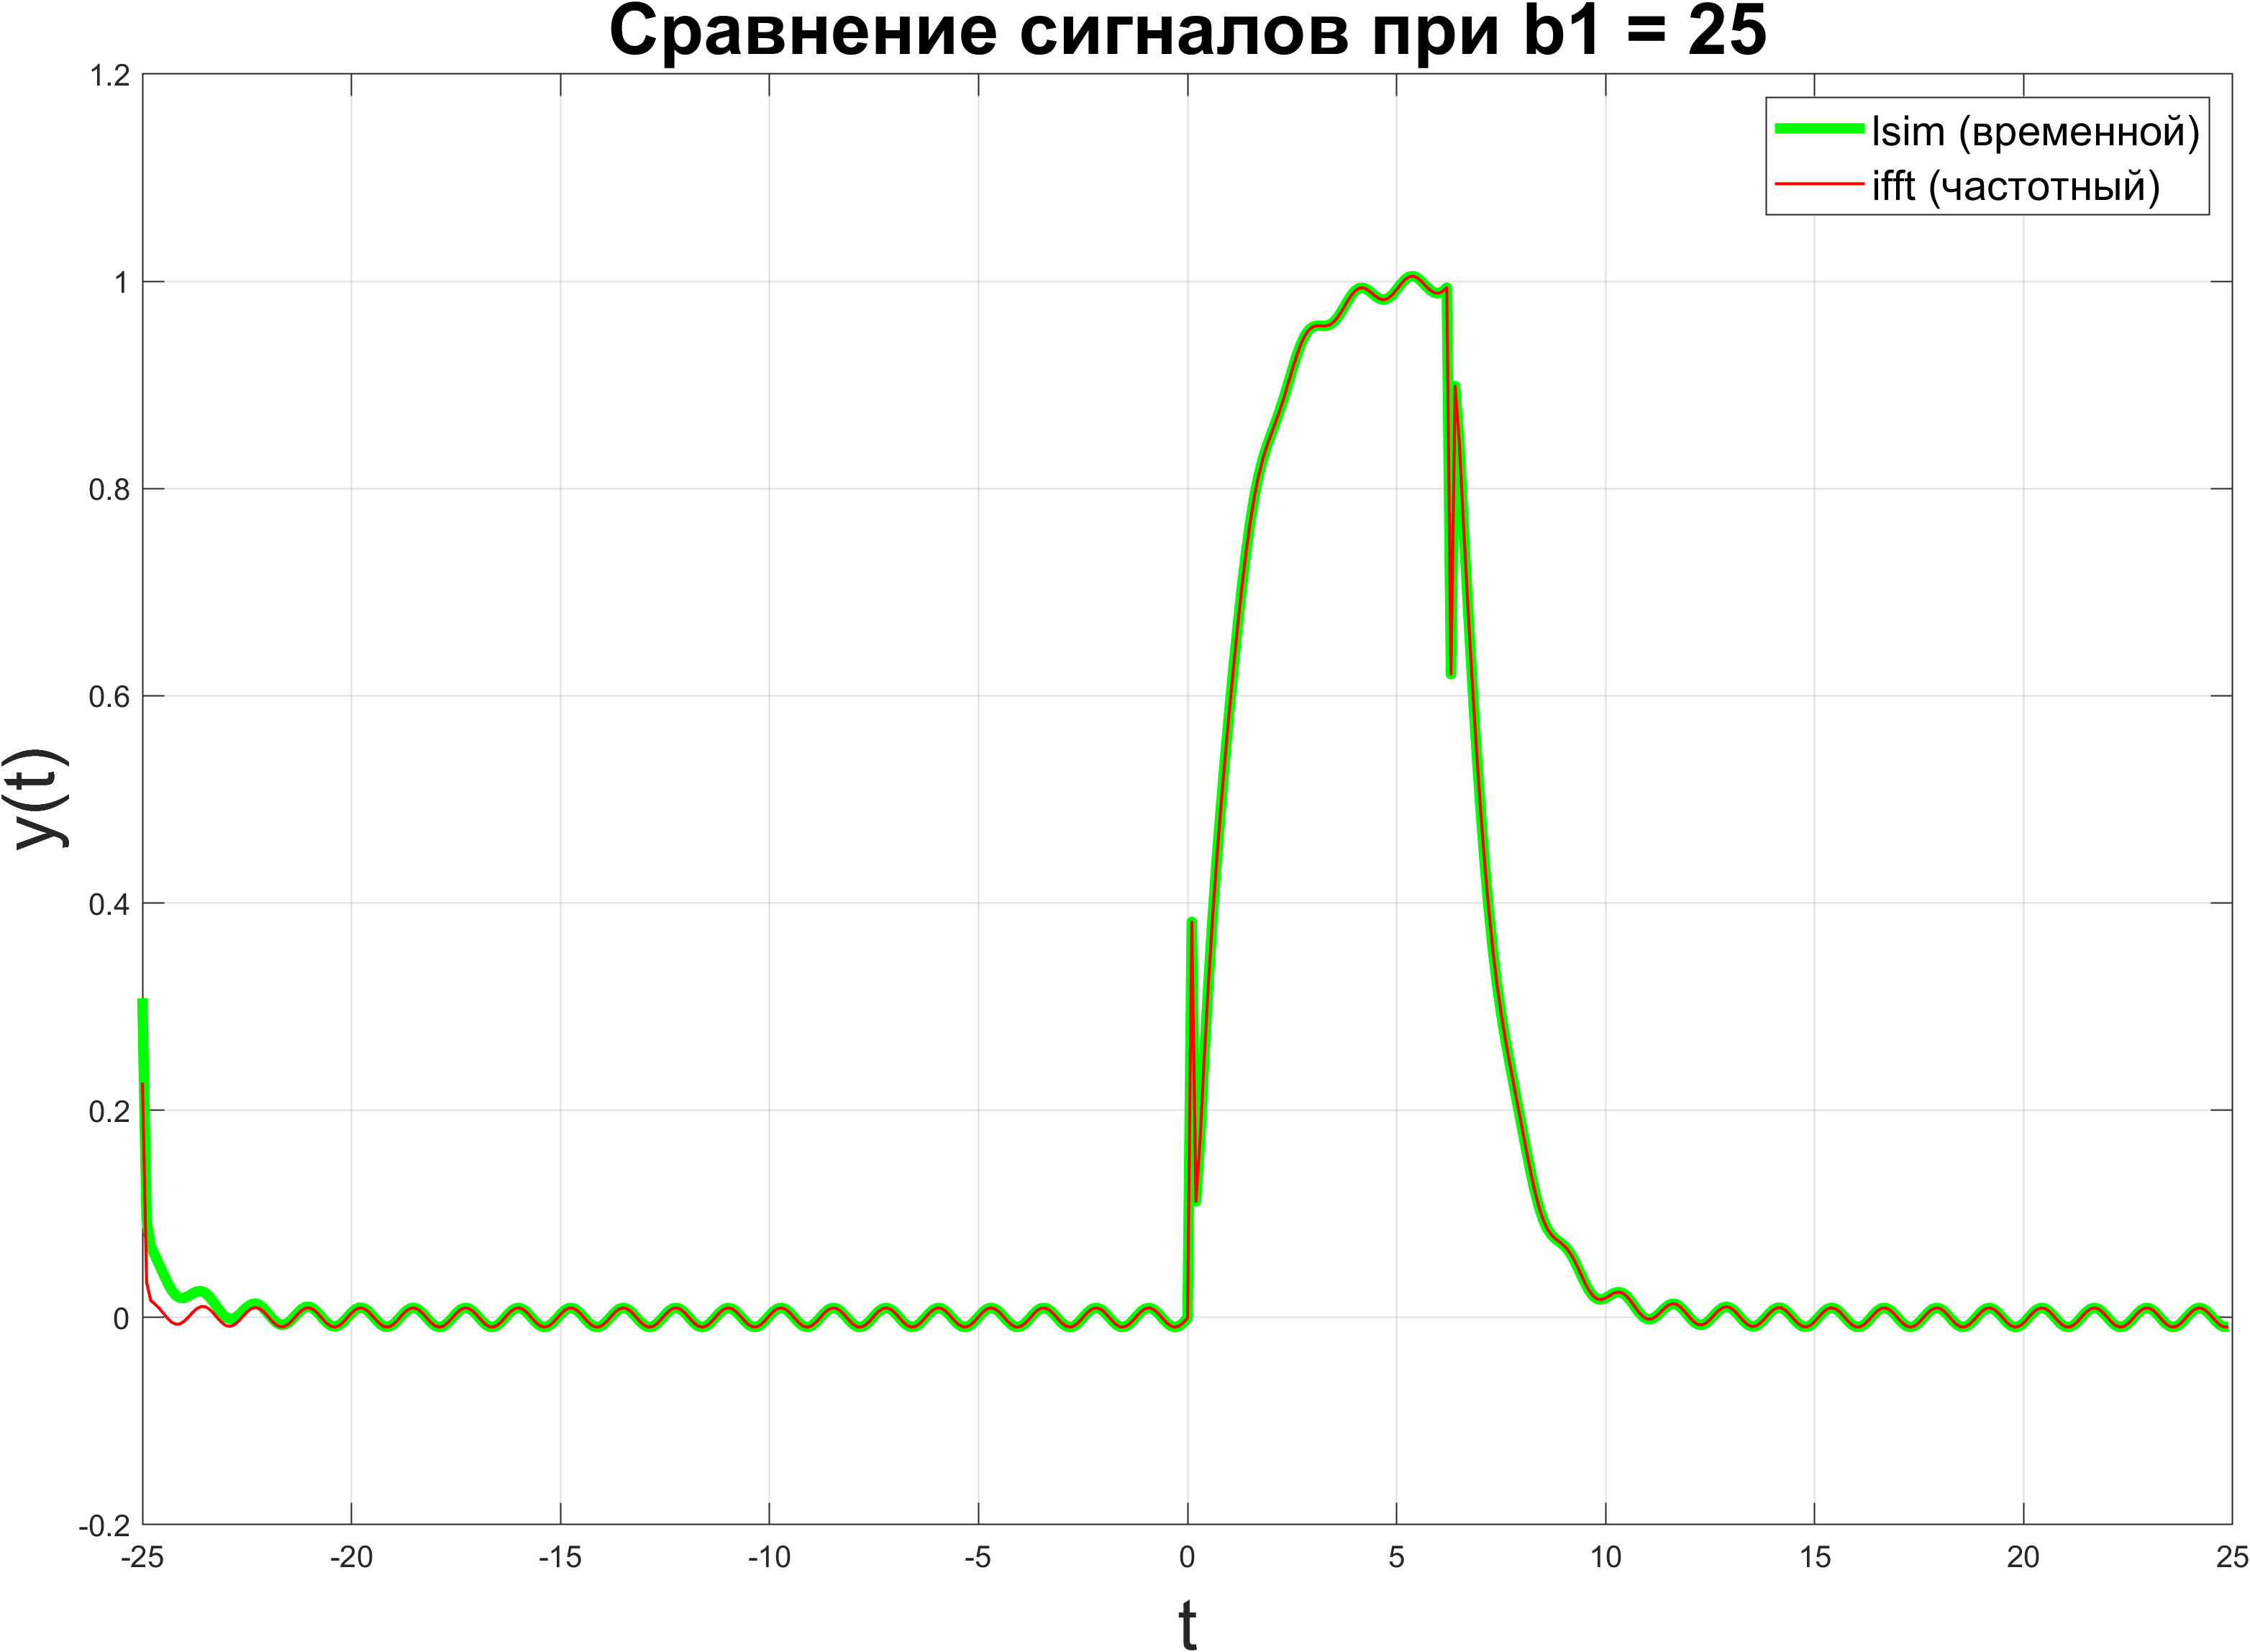
\includegraphics[width=0.92\textwidth, keepaspectratio]{images2/filter_transf_b1_25.png}
    \caption{Сравнение методов при $b_1 = 25$}
\end{figure}
\newpage

Модули Фурье-образов исходного, зашумленного и фильтрованного сигналов:
\begin{figure}[H]
    \centering
    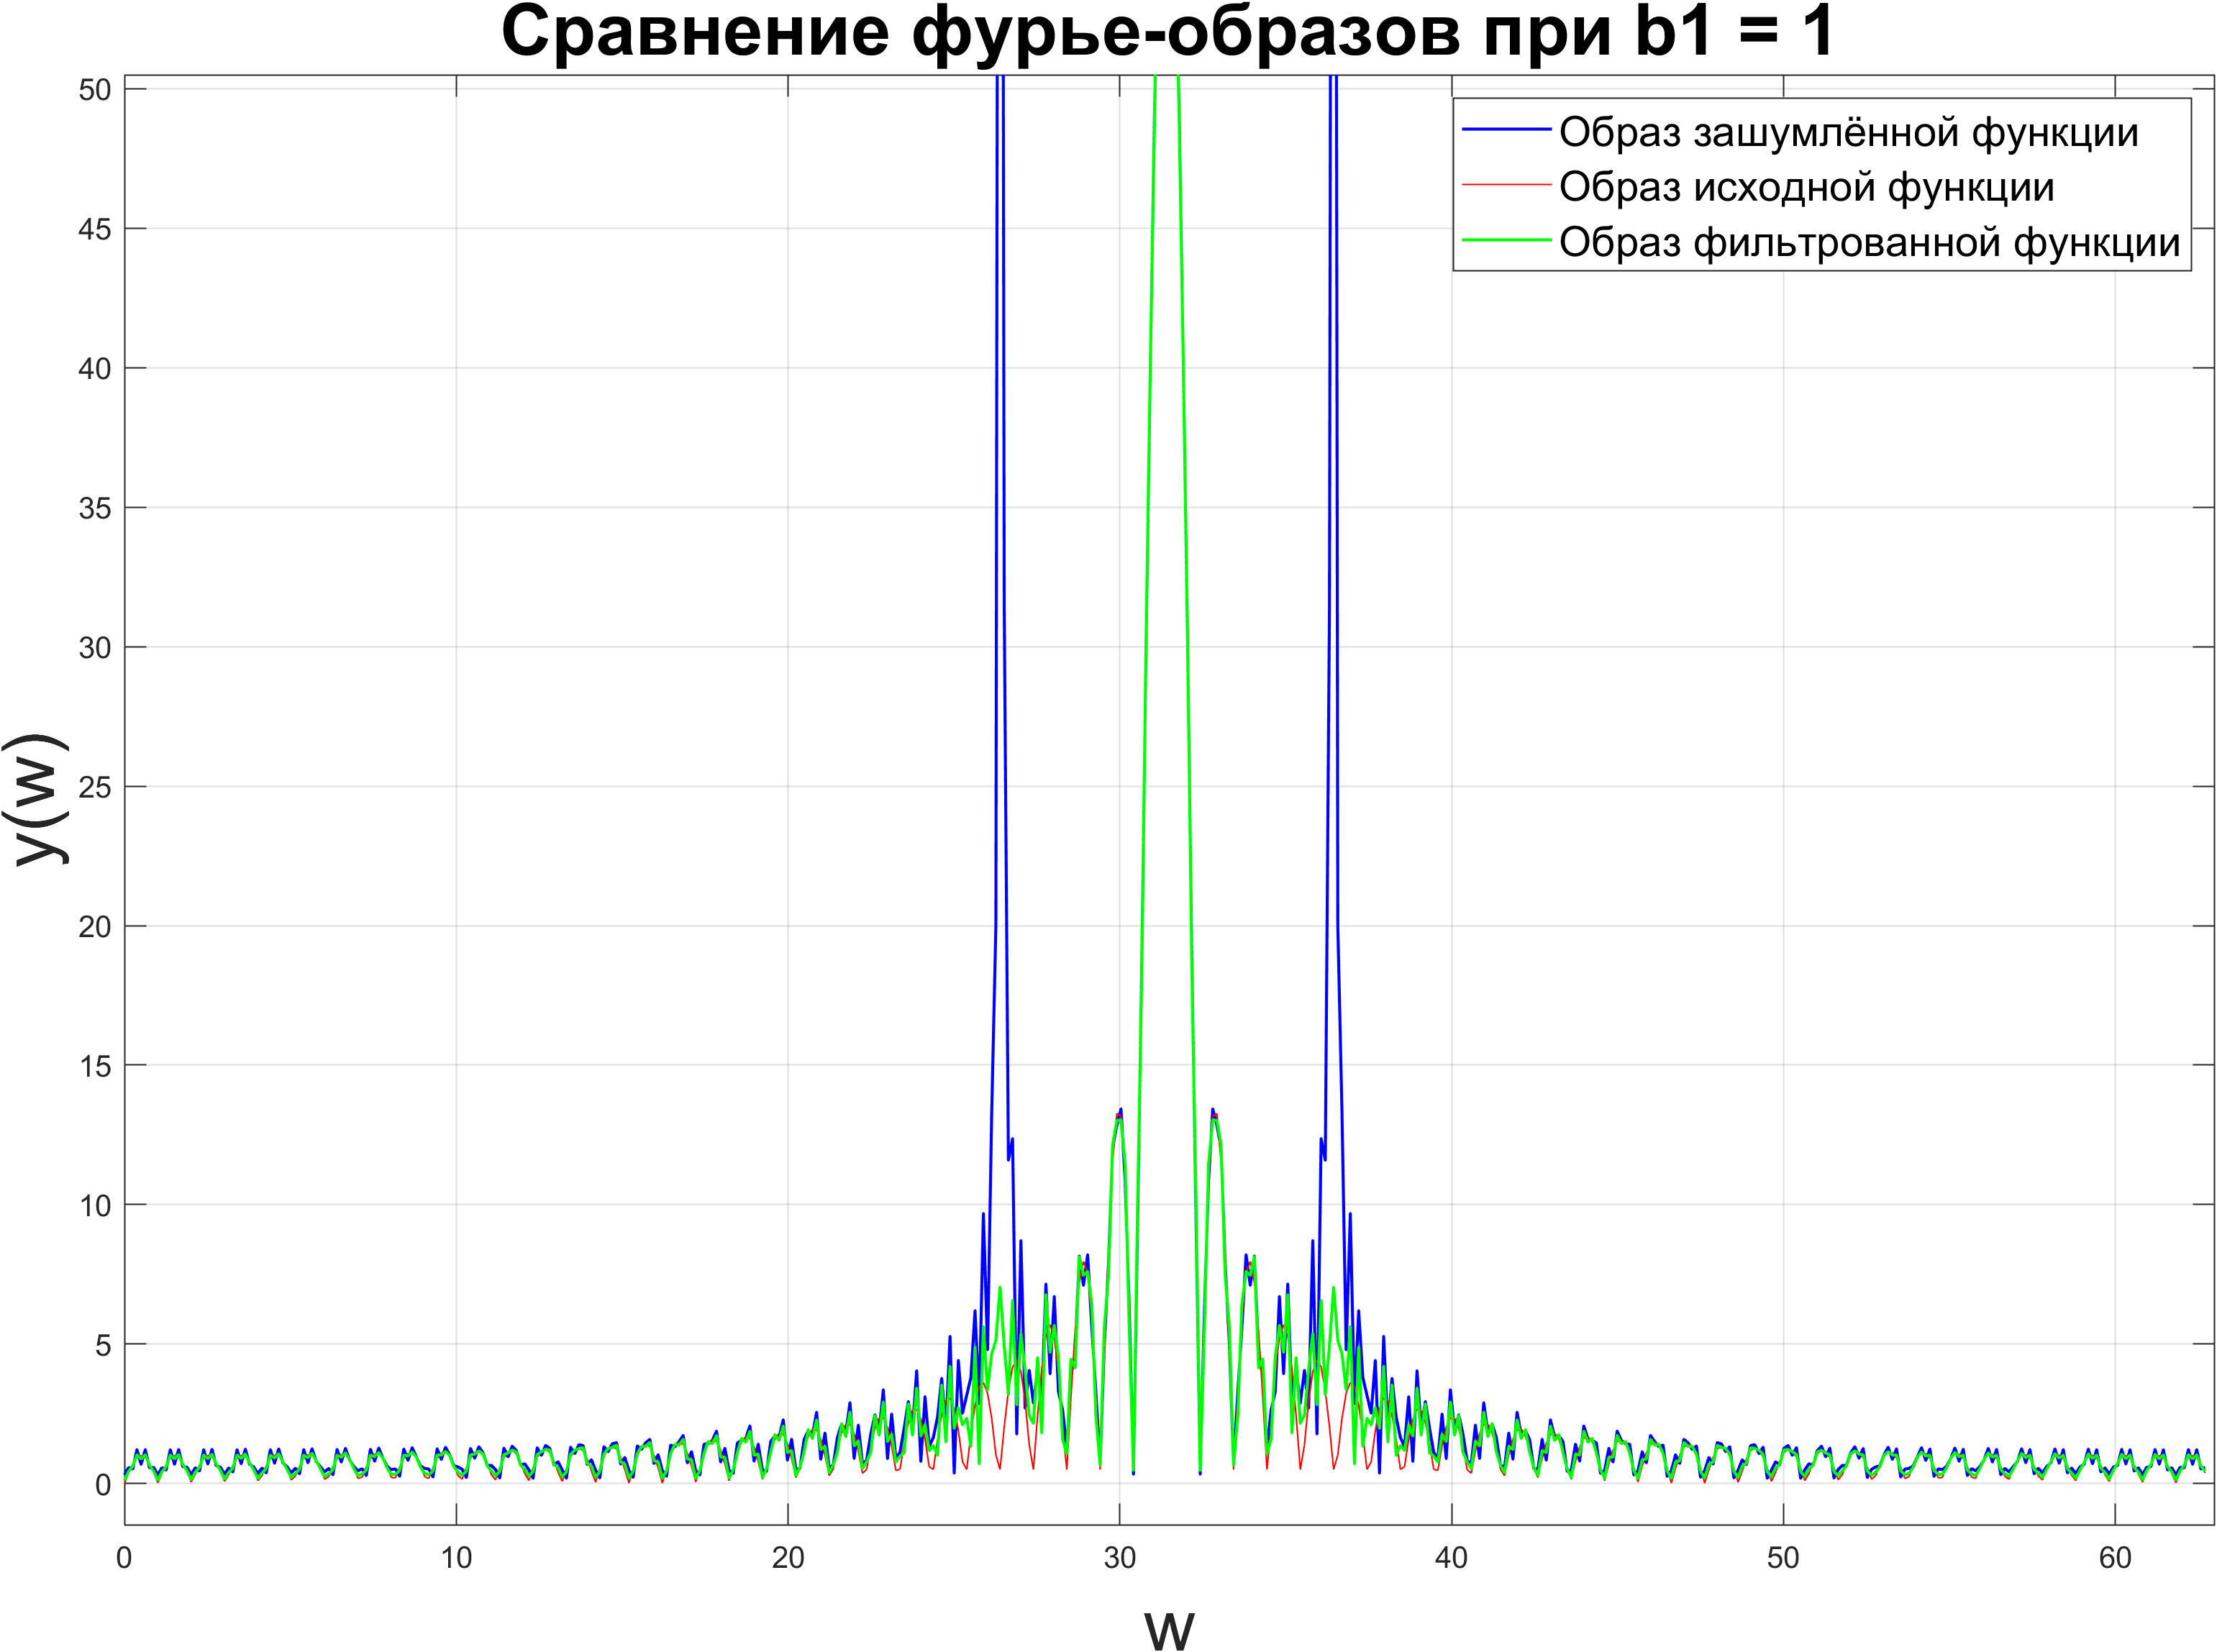
\includegraphics[width=0.85\textwidth, keepaspectratio]{images2/fur_imgs_g_b1_1.png}
    \caption{Фурье-образы двух методов при $b_1 = 1$}
\end{figure}
\begin{figure}[H]
    \centering
    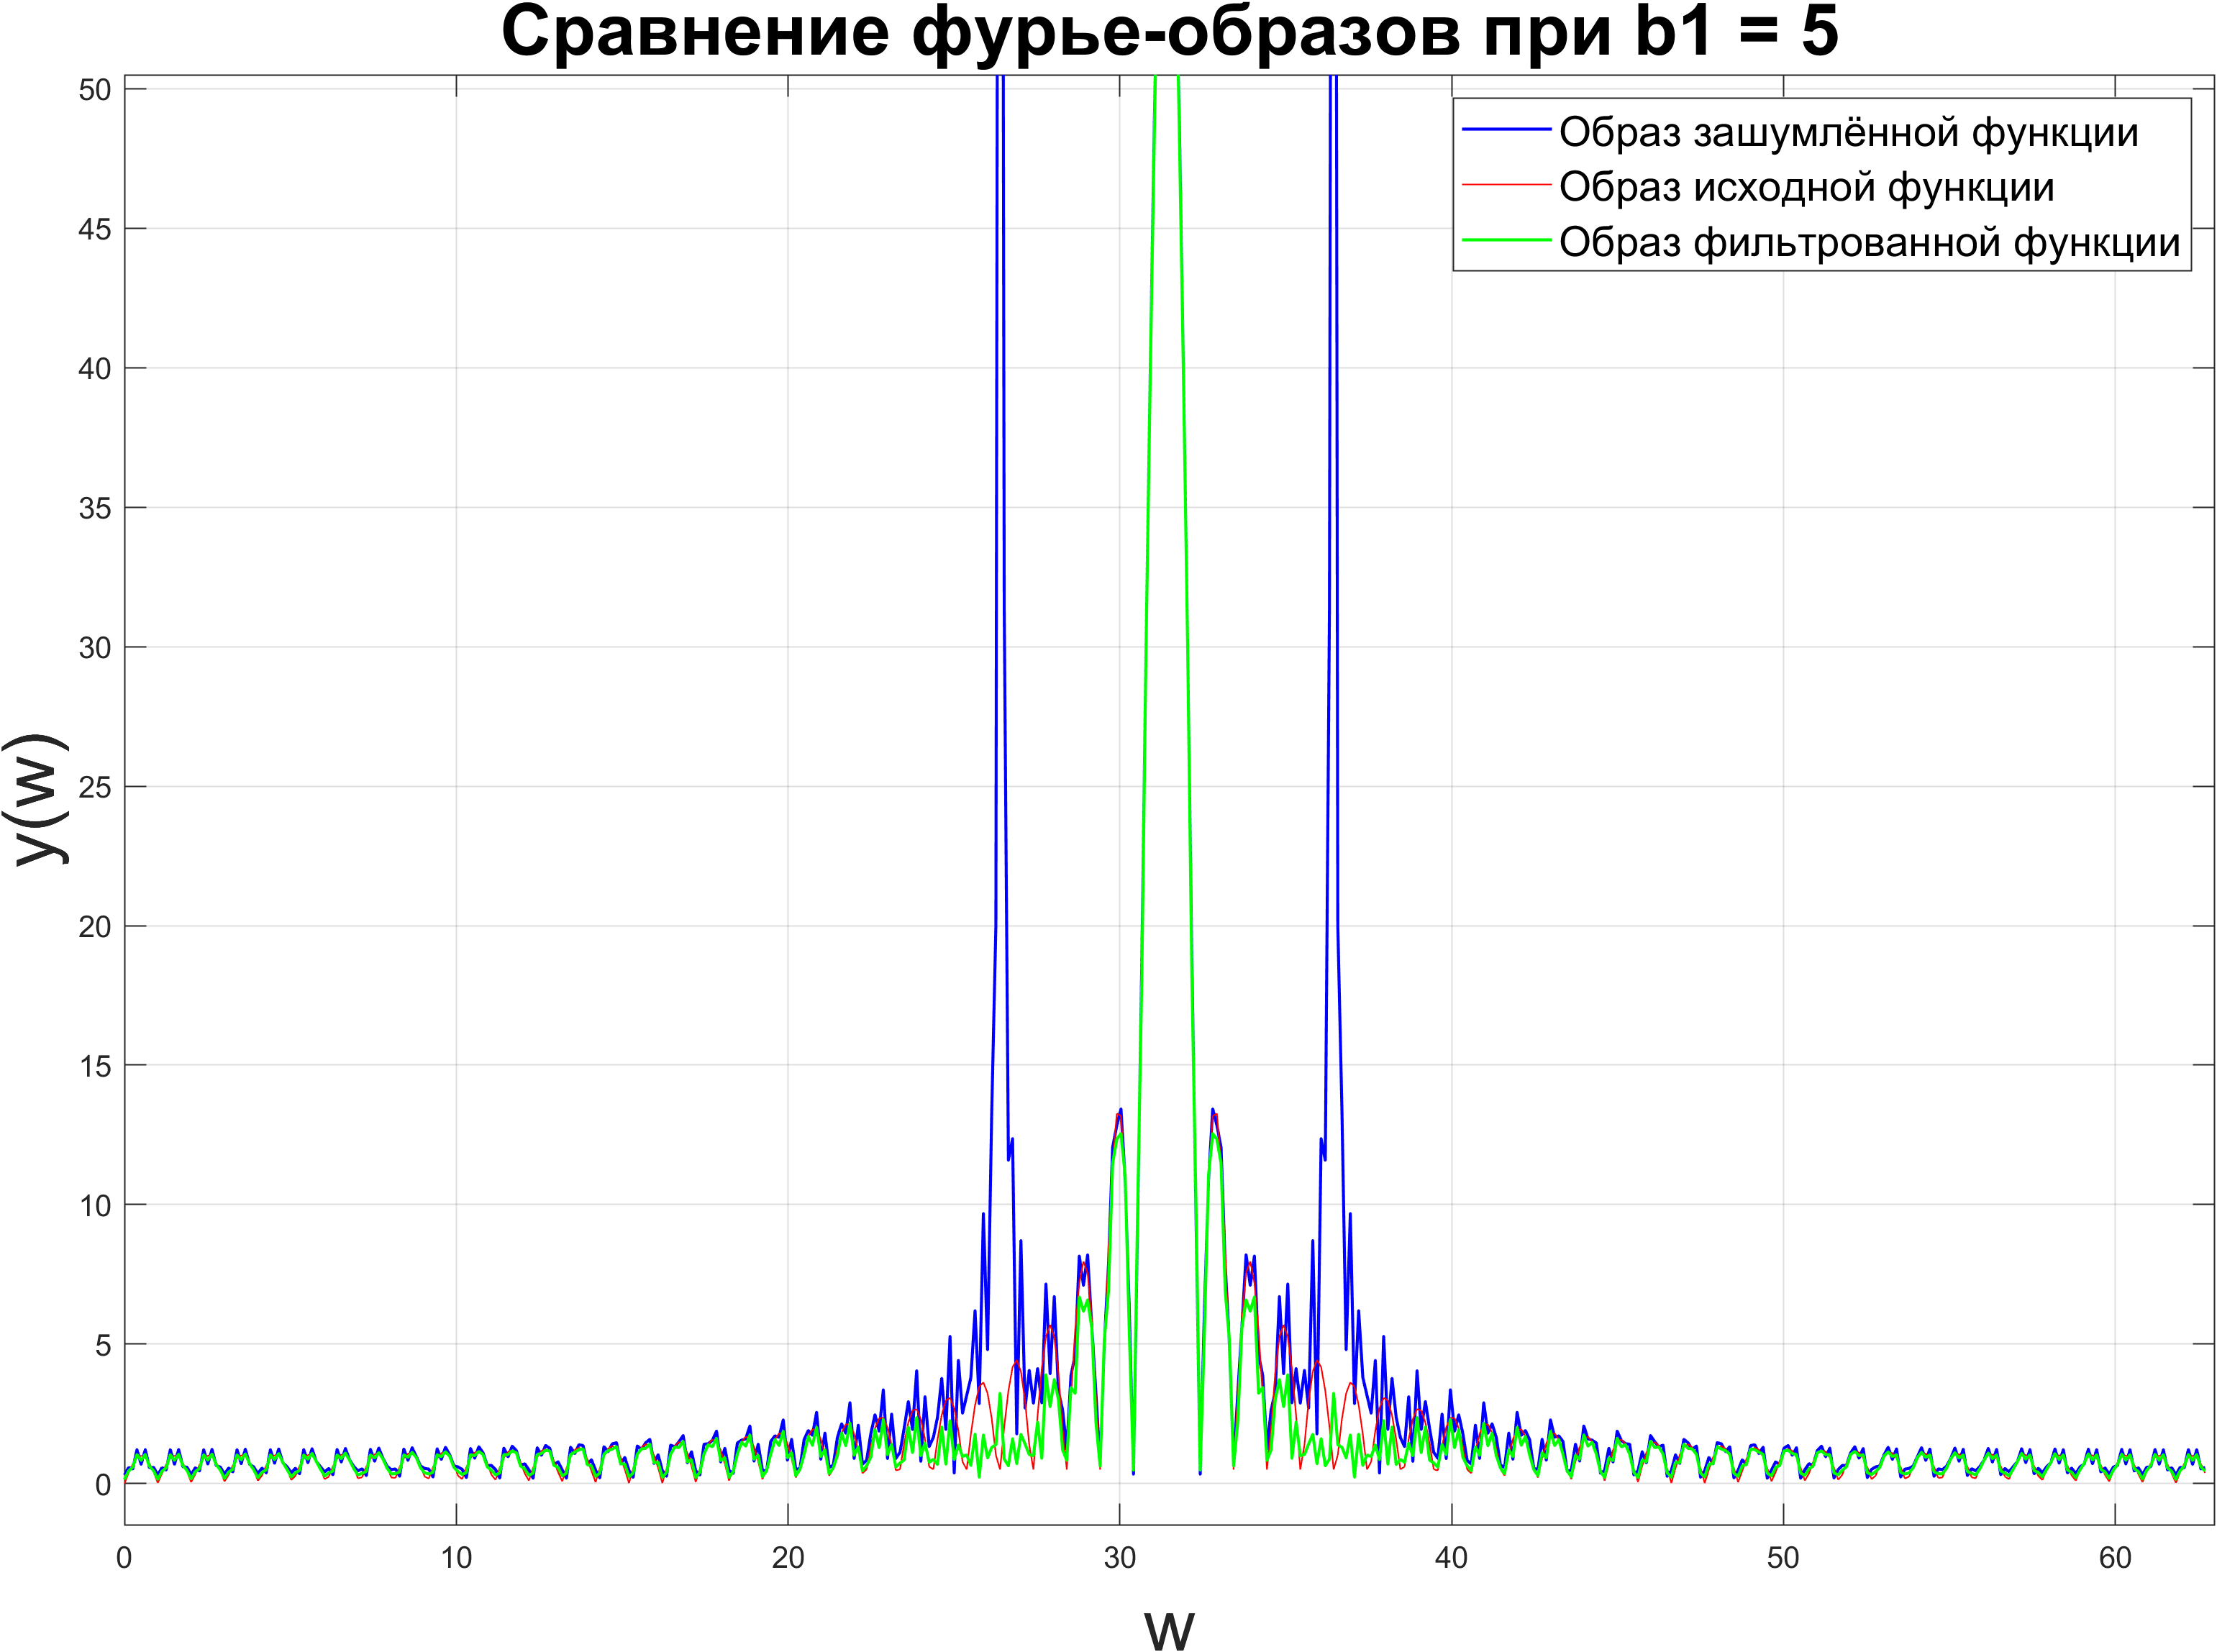
\includegraphics[width=0.85\textwidth, keepaspectratio]{images2/fur_imgs_g_b1_5.png}
    \caption{Фурье-образы двух методов при $b_1 = 5$}
\end{figure}
\newpage

\begin{figure}[H]
    \centering
    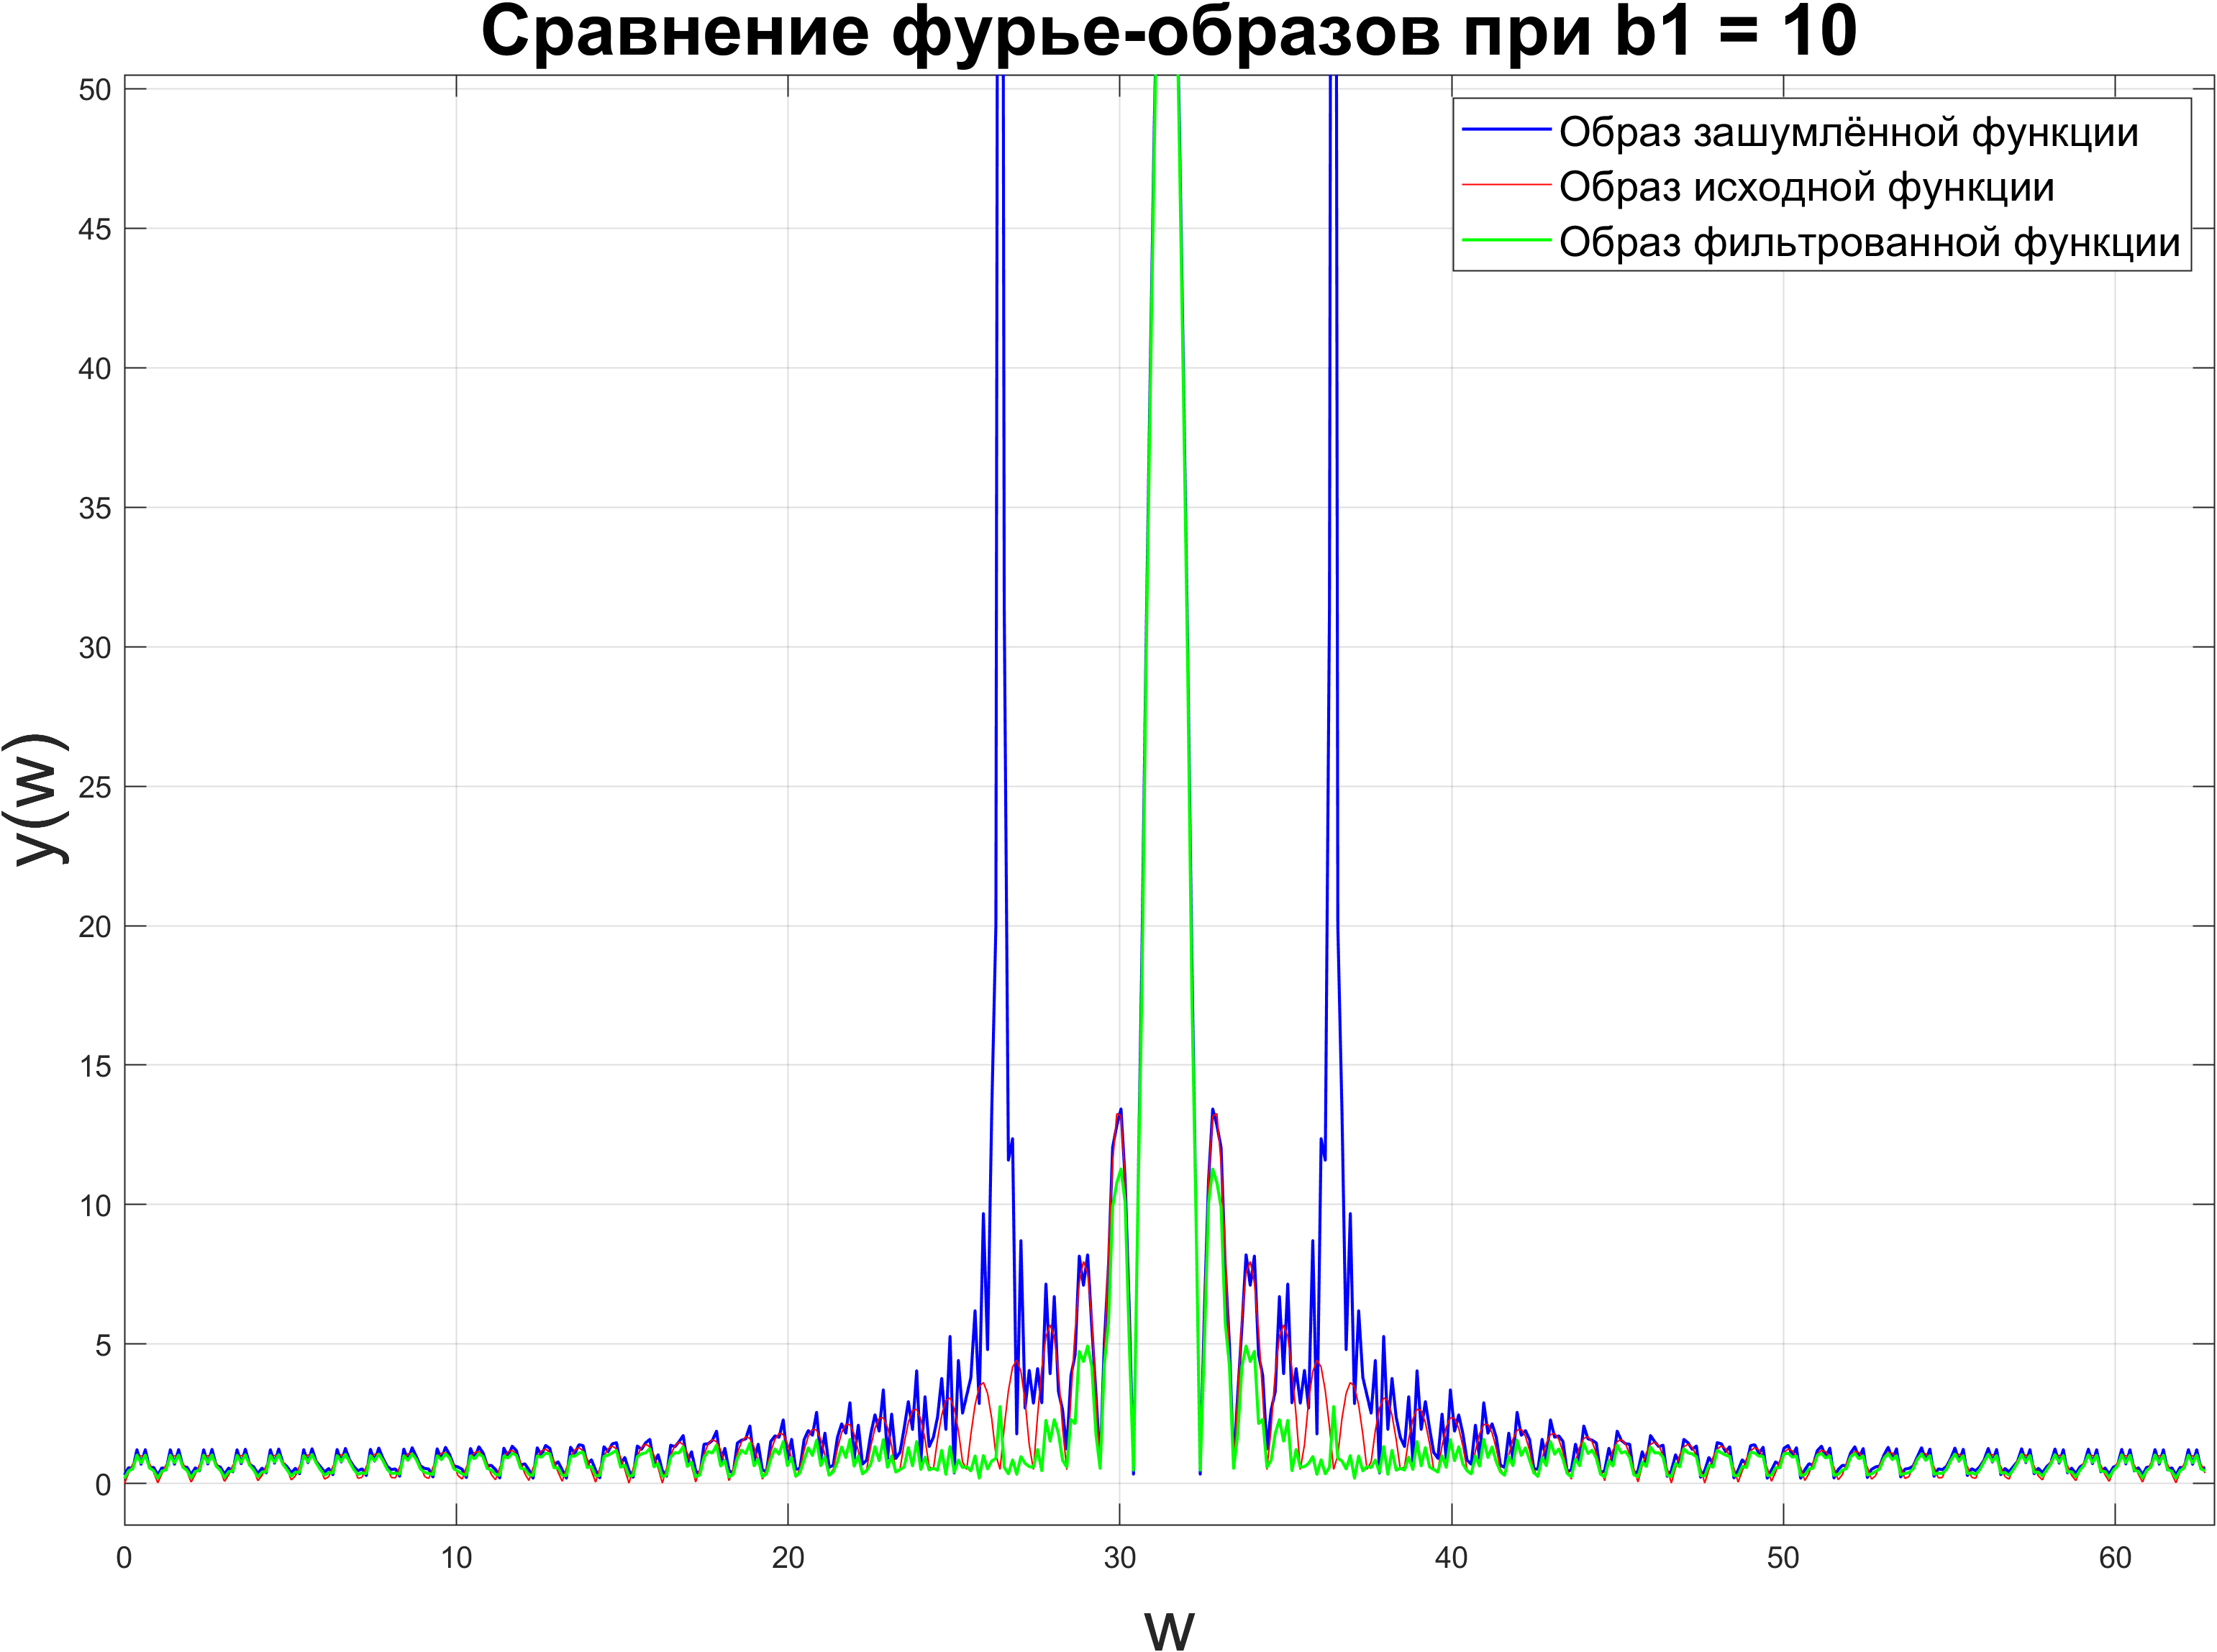
\includegraphics[width=0.90\textwidth, keepaspectratio]{images2/fur_imgs_g_b1_10.png}
    \caption{Фурье-образы двух методов при $b_1 = 10$}
\end{figure}
\begin{figure}[H]
    \centering
    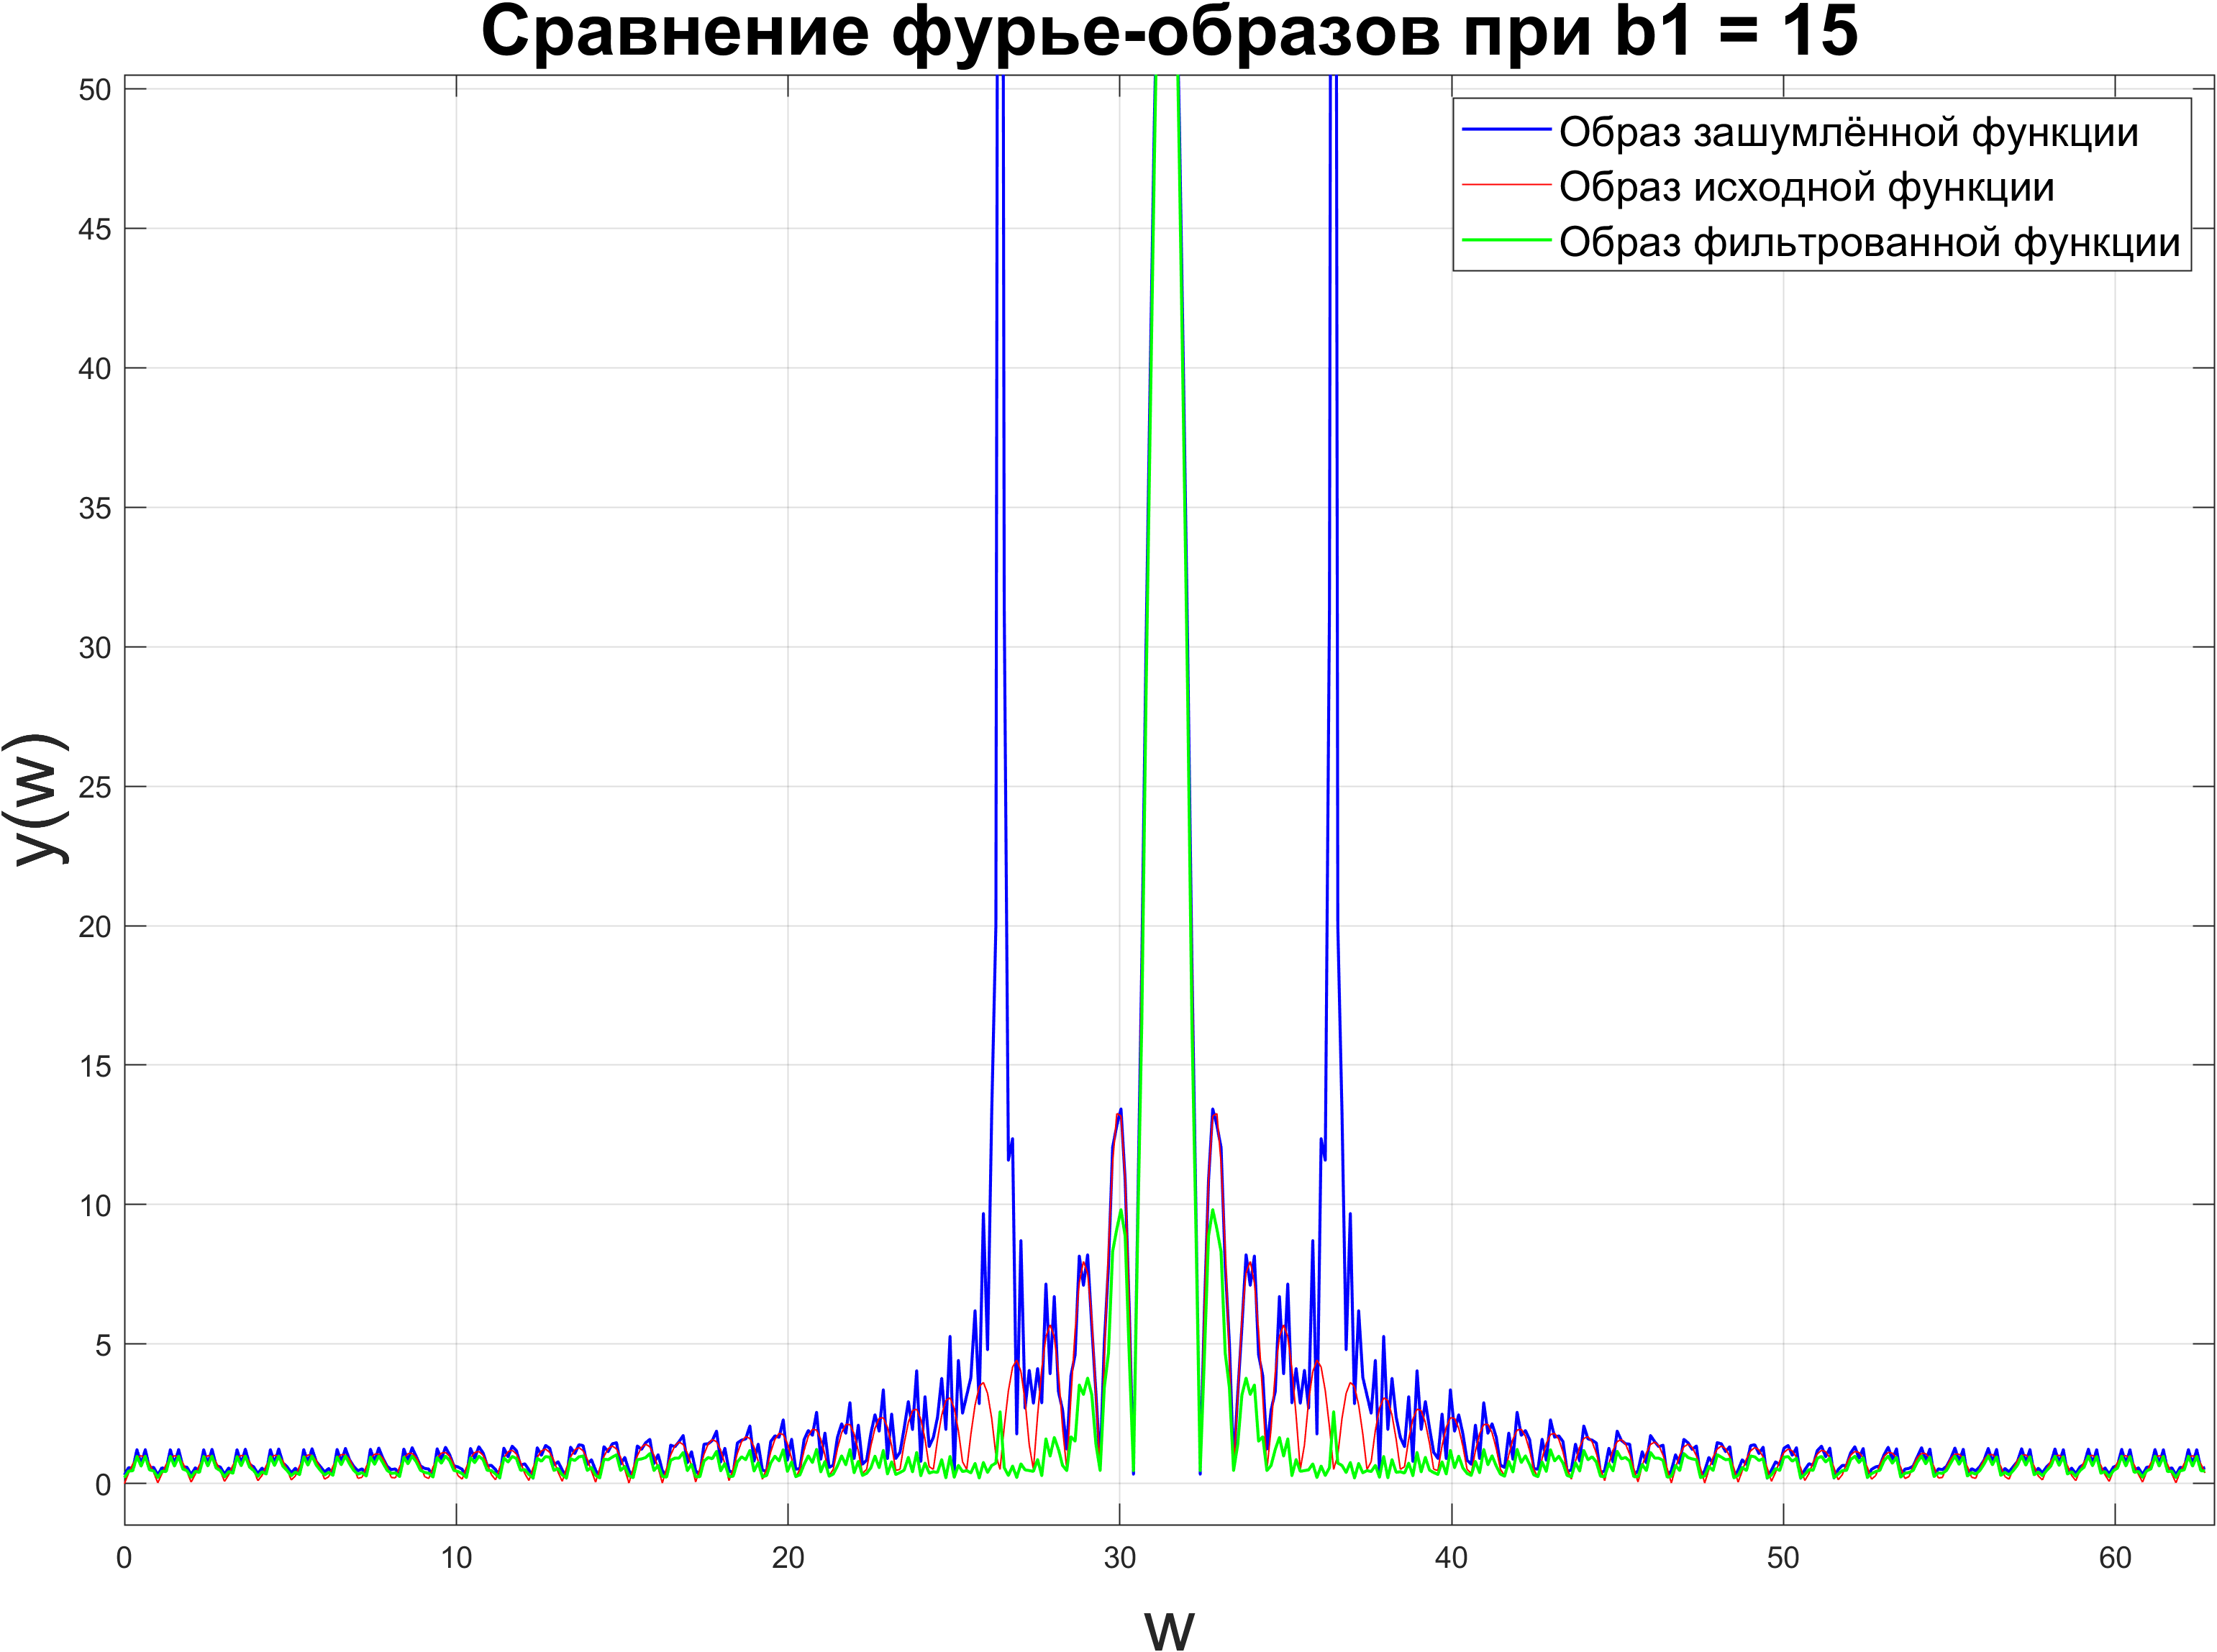
\includegraphics[width=0.90\textwidth, keepaspectratio]{images2/fur_imgs_g_b1_15.png}
    \caption{Фурье-образы двух методов при $b_1 = 15$}
\end{figure}
\newpage

\begin{figure}[H]
    \centering
    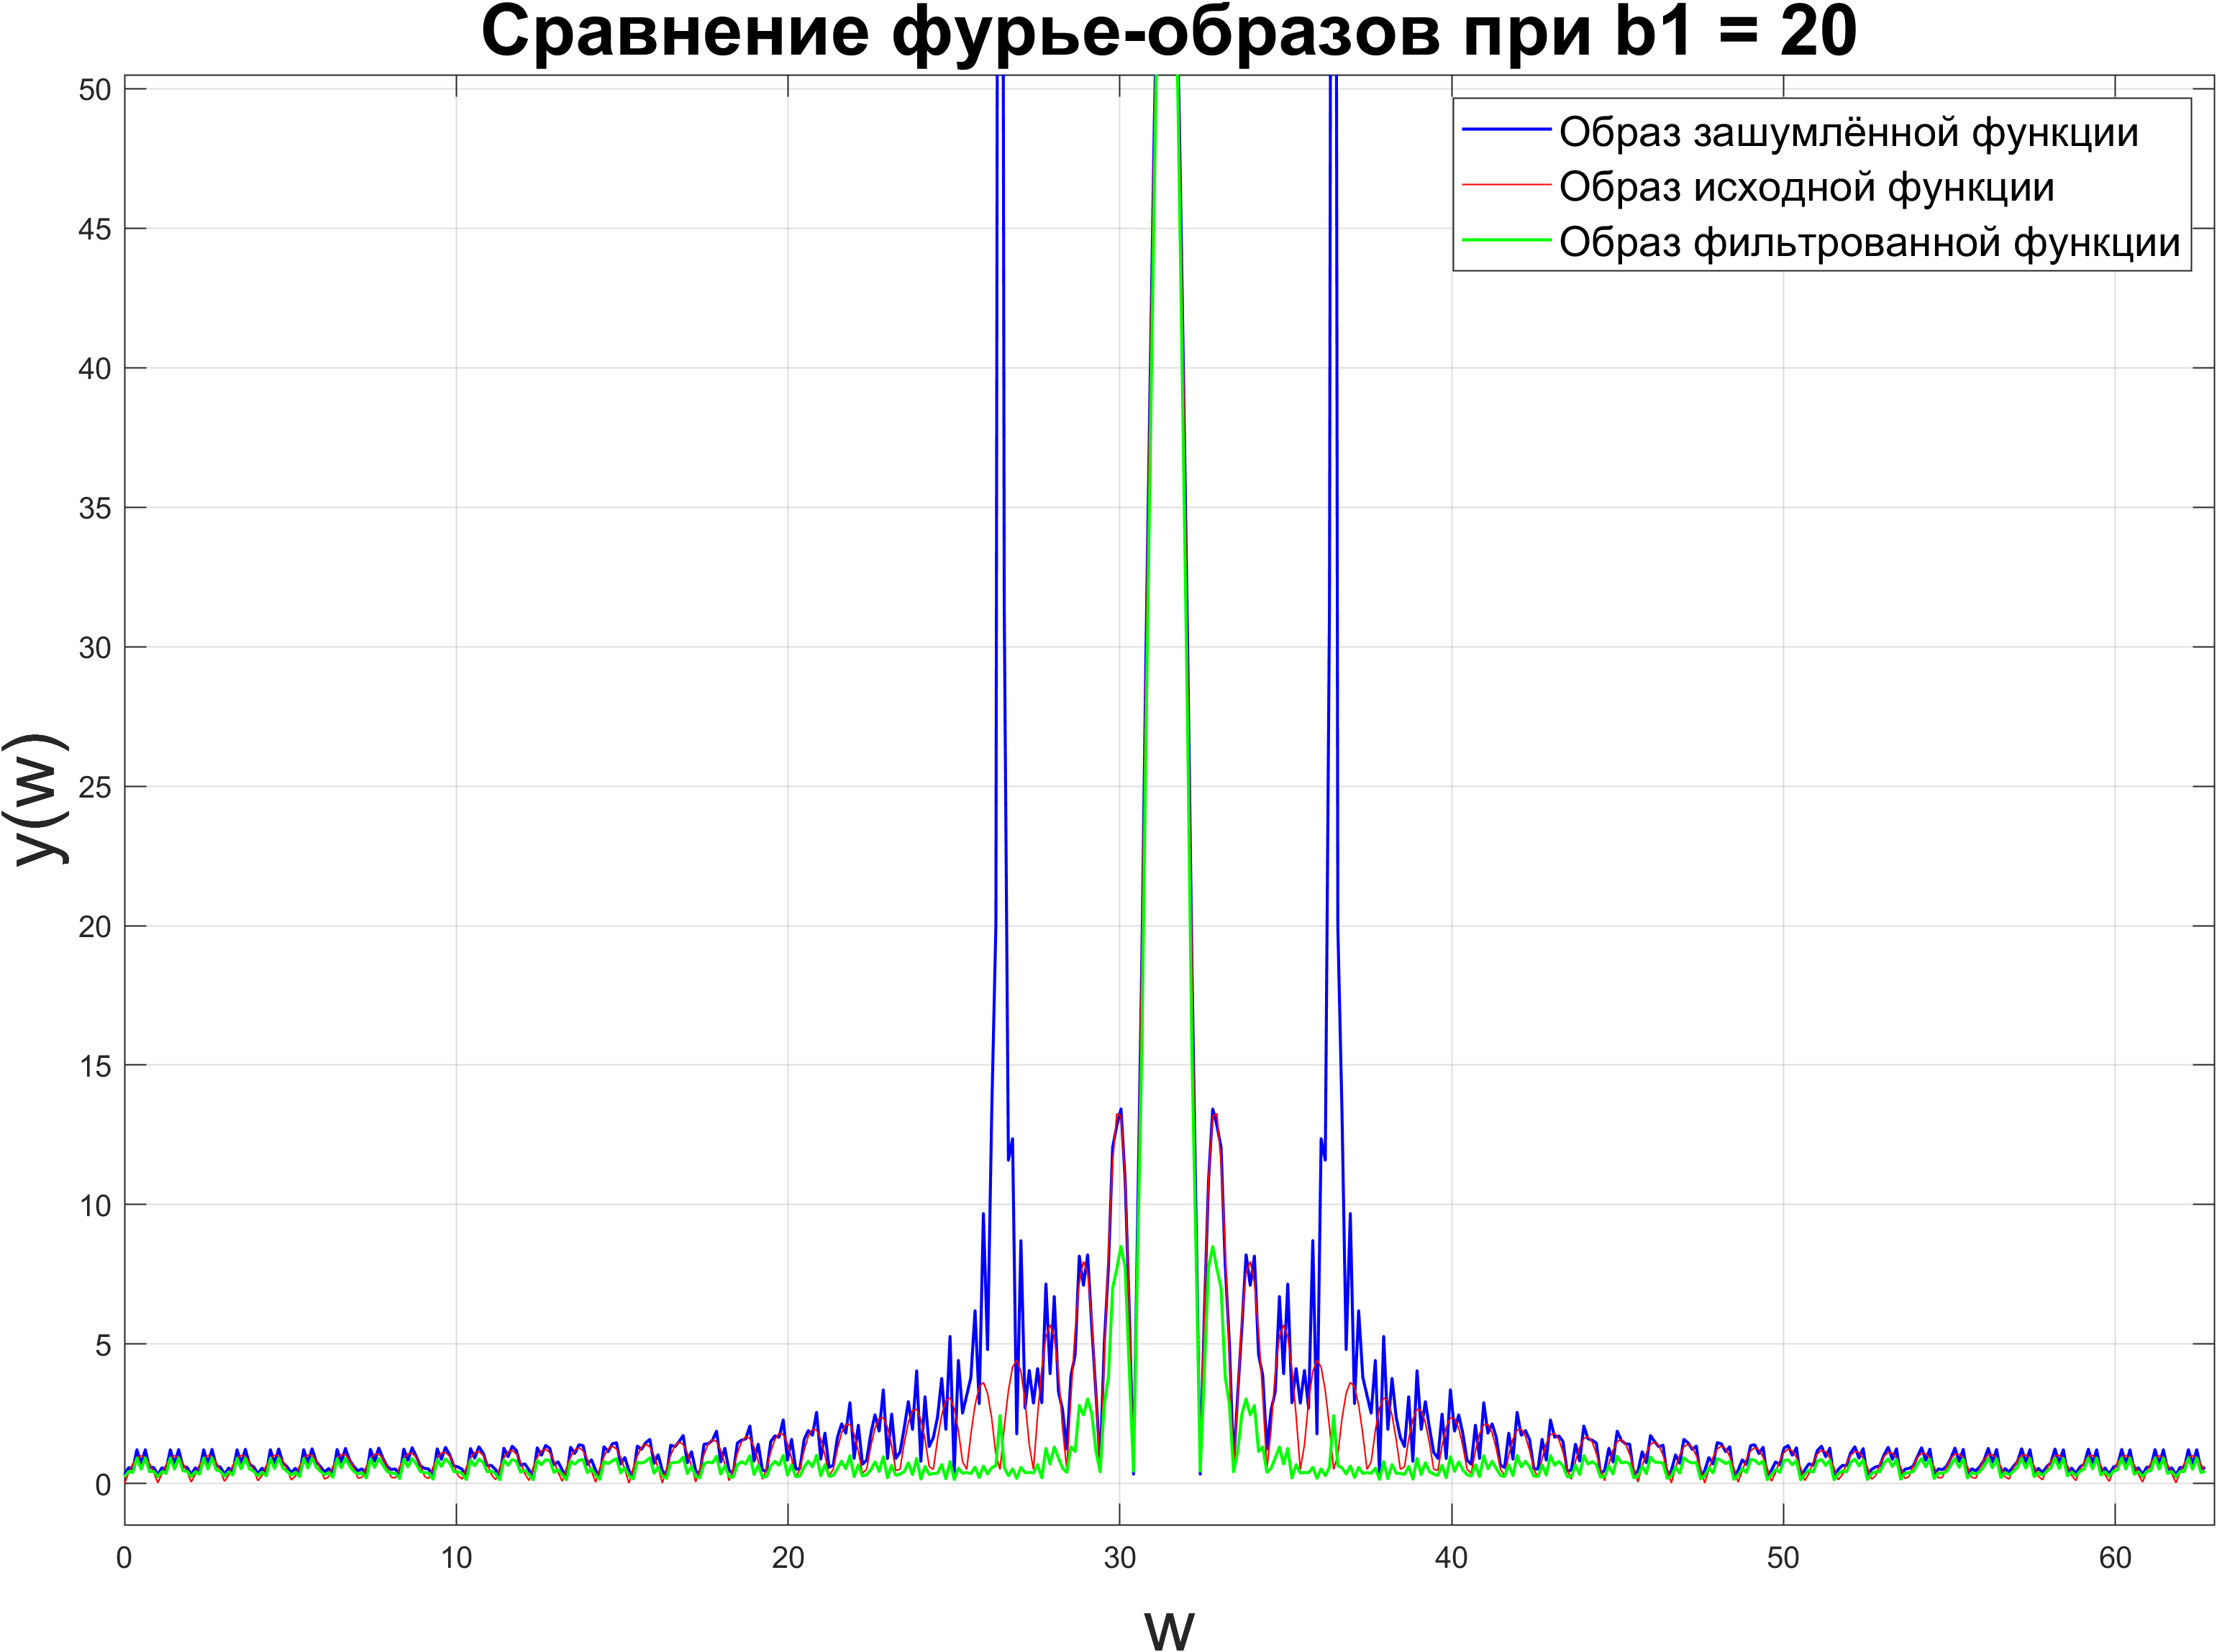
\includegraphics[width=0.90\textwidth, keepaspectratio]{images2/fur_imgs_g_b1_20.png}
    \caption{Фурье-образы двух методов при $b_1 = 20$}
\end{figure}
\begin{figure}[H]
    \centering
    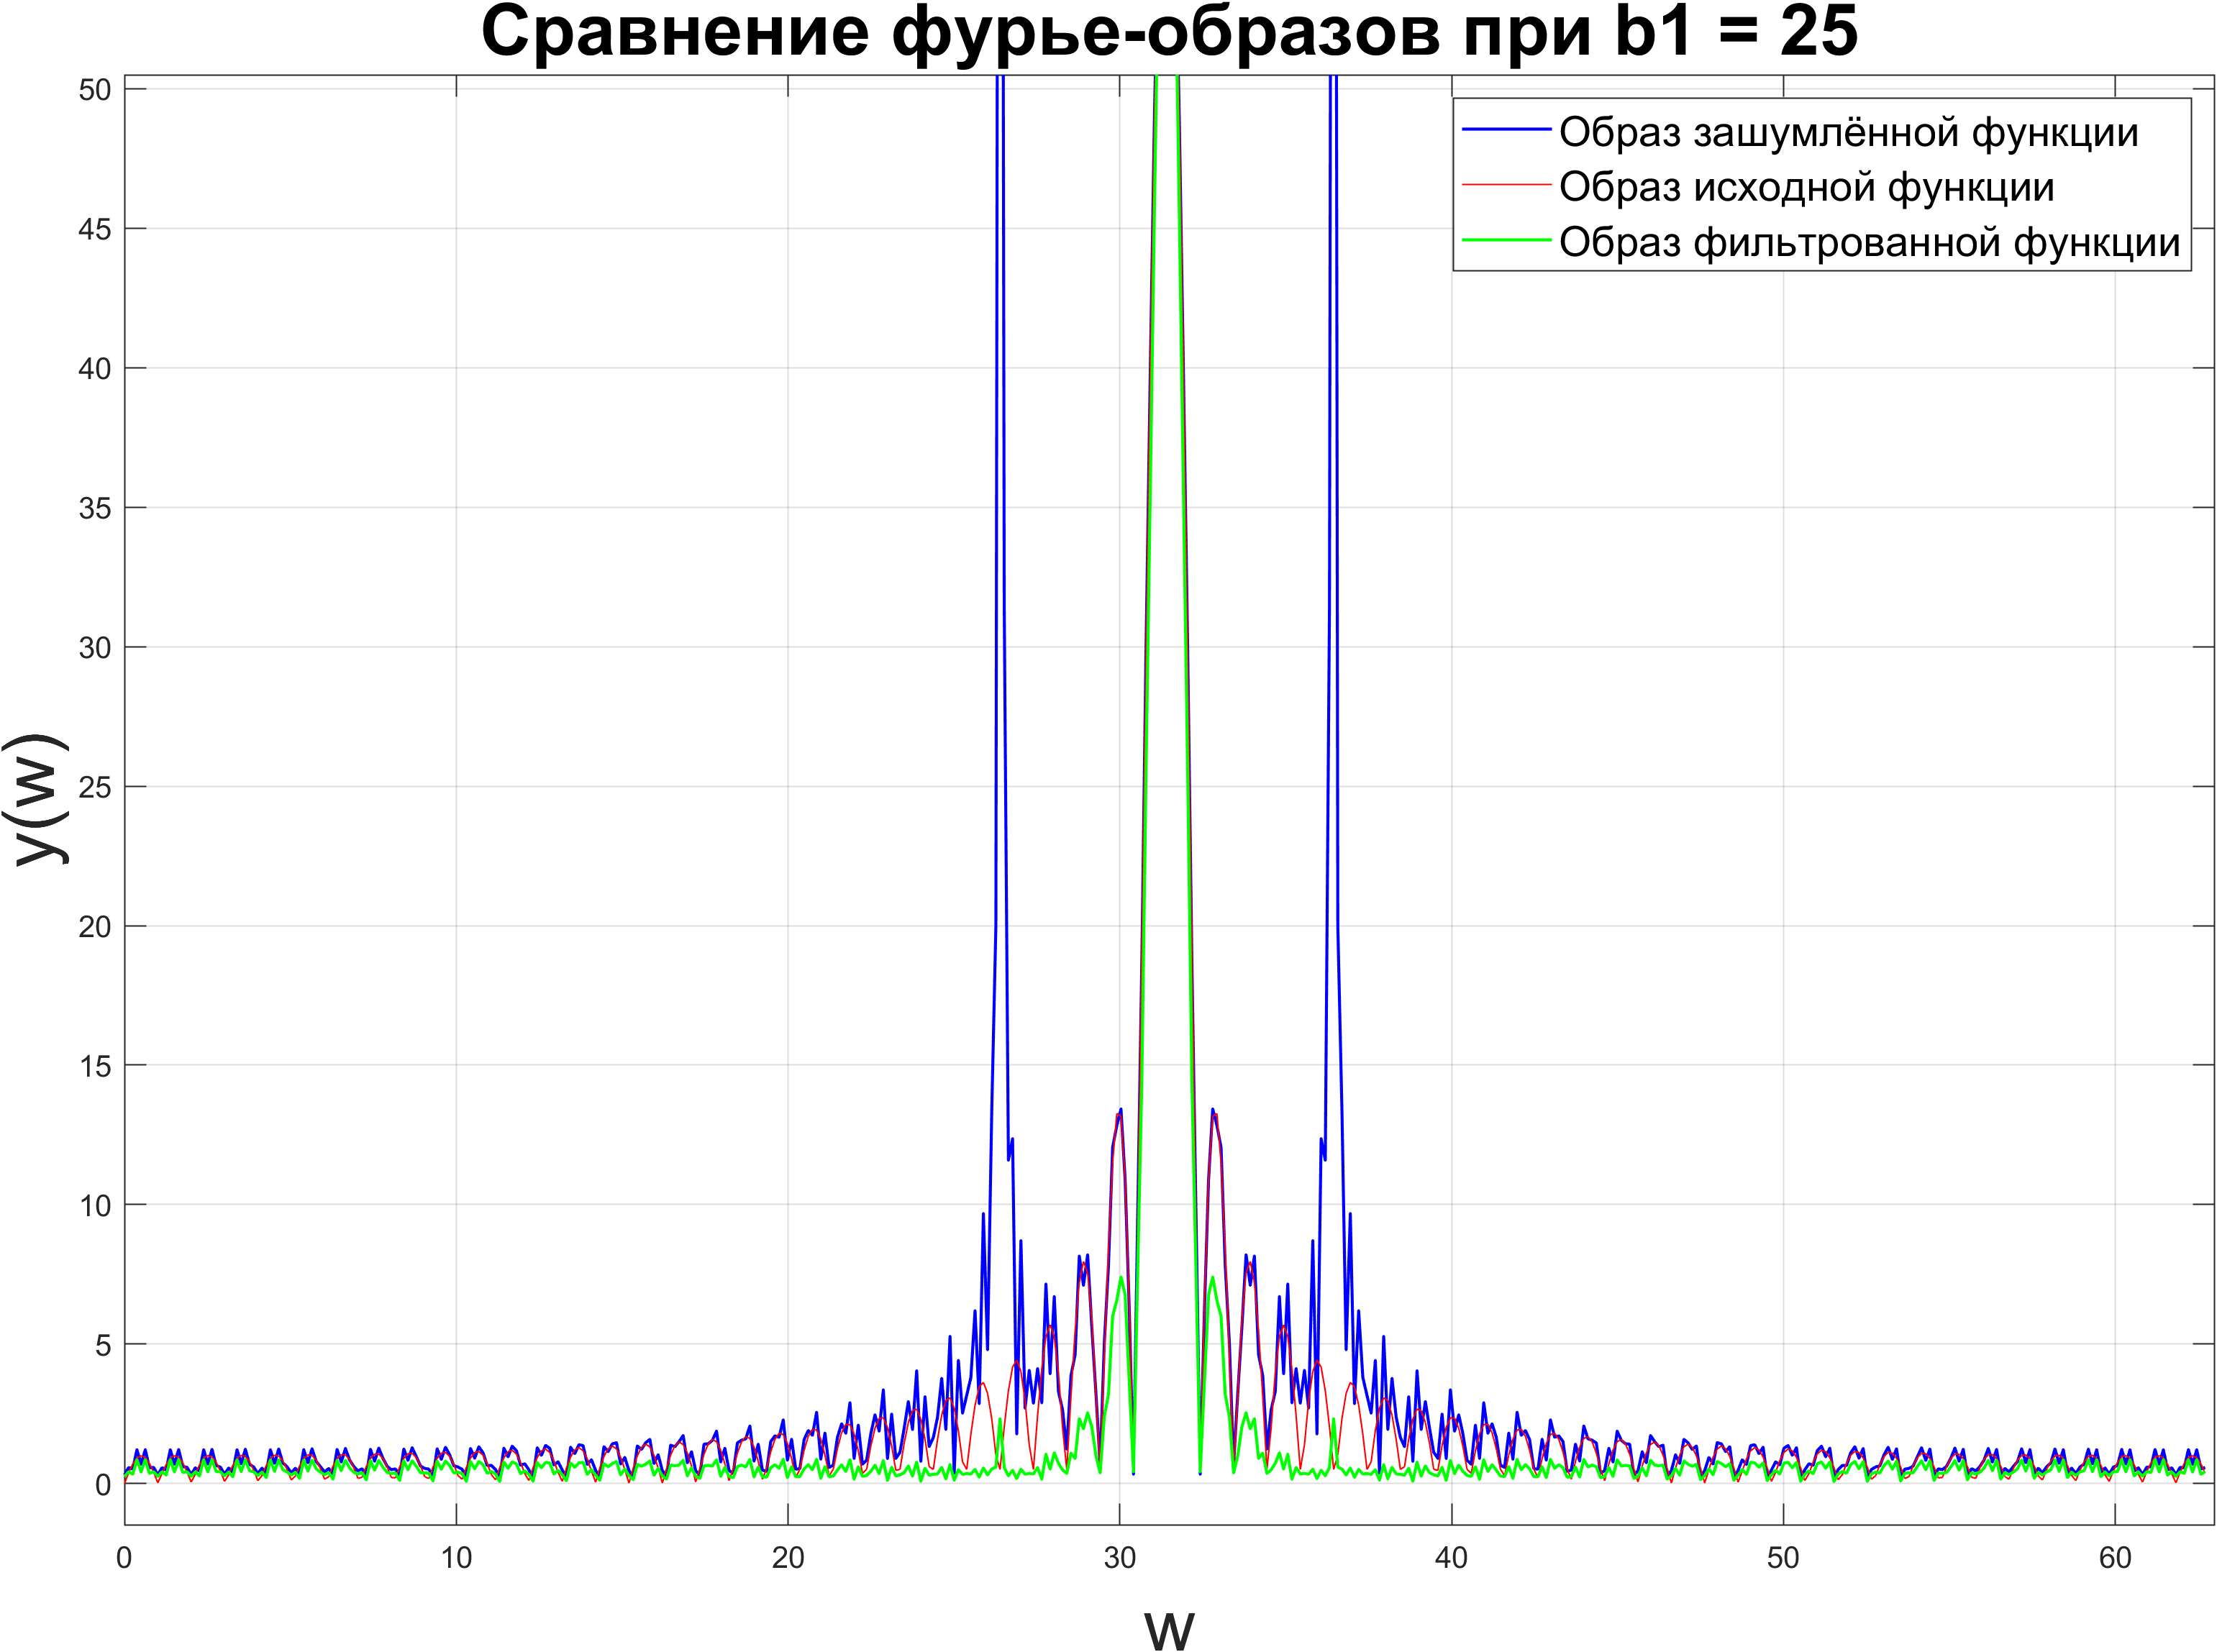
\includegraphics[width=0.90\textwidth, keepaspectratio]{images2/fur_imgs_g_b1_25.png}
    \caption{Фурье-образы двух методов при $b_1 = 25$}
\end{figure}
\newpage

Сравнение модулей Фурье-образа фильрованной функции и произведения передаточной функции на Фурье-образ зашумленной функции
\begin{figure}[H]
    \centering
    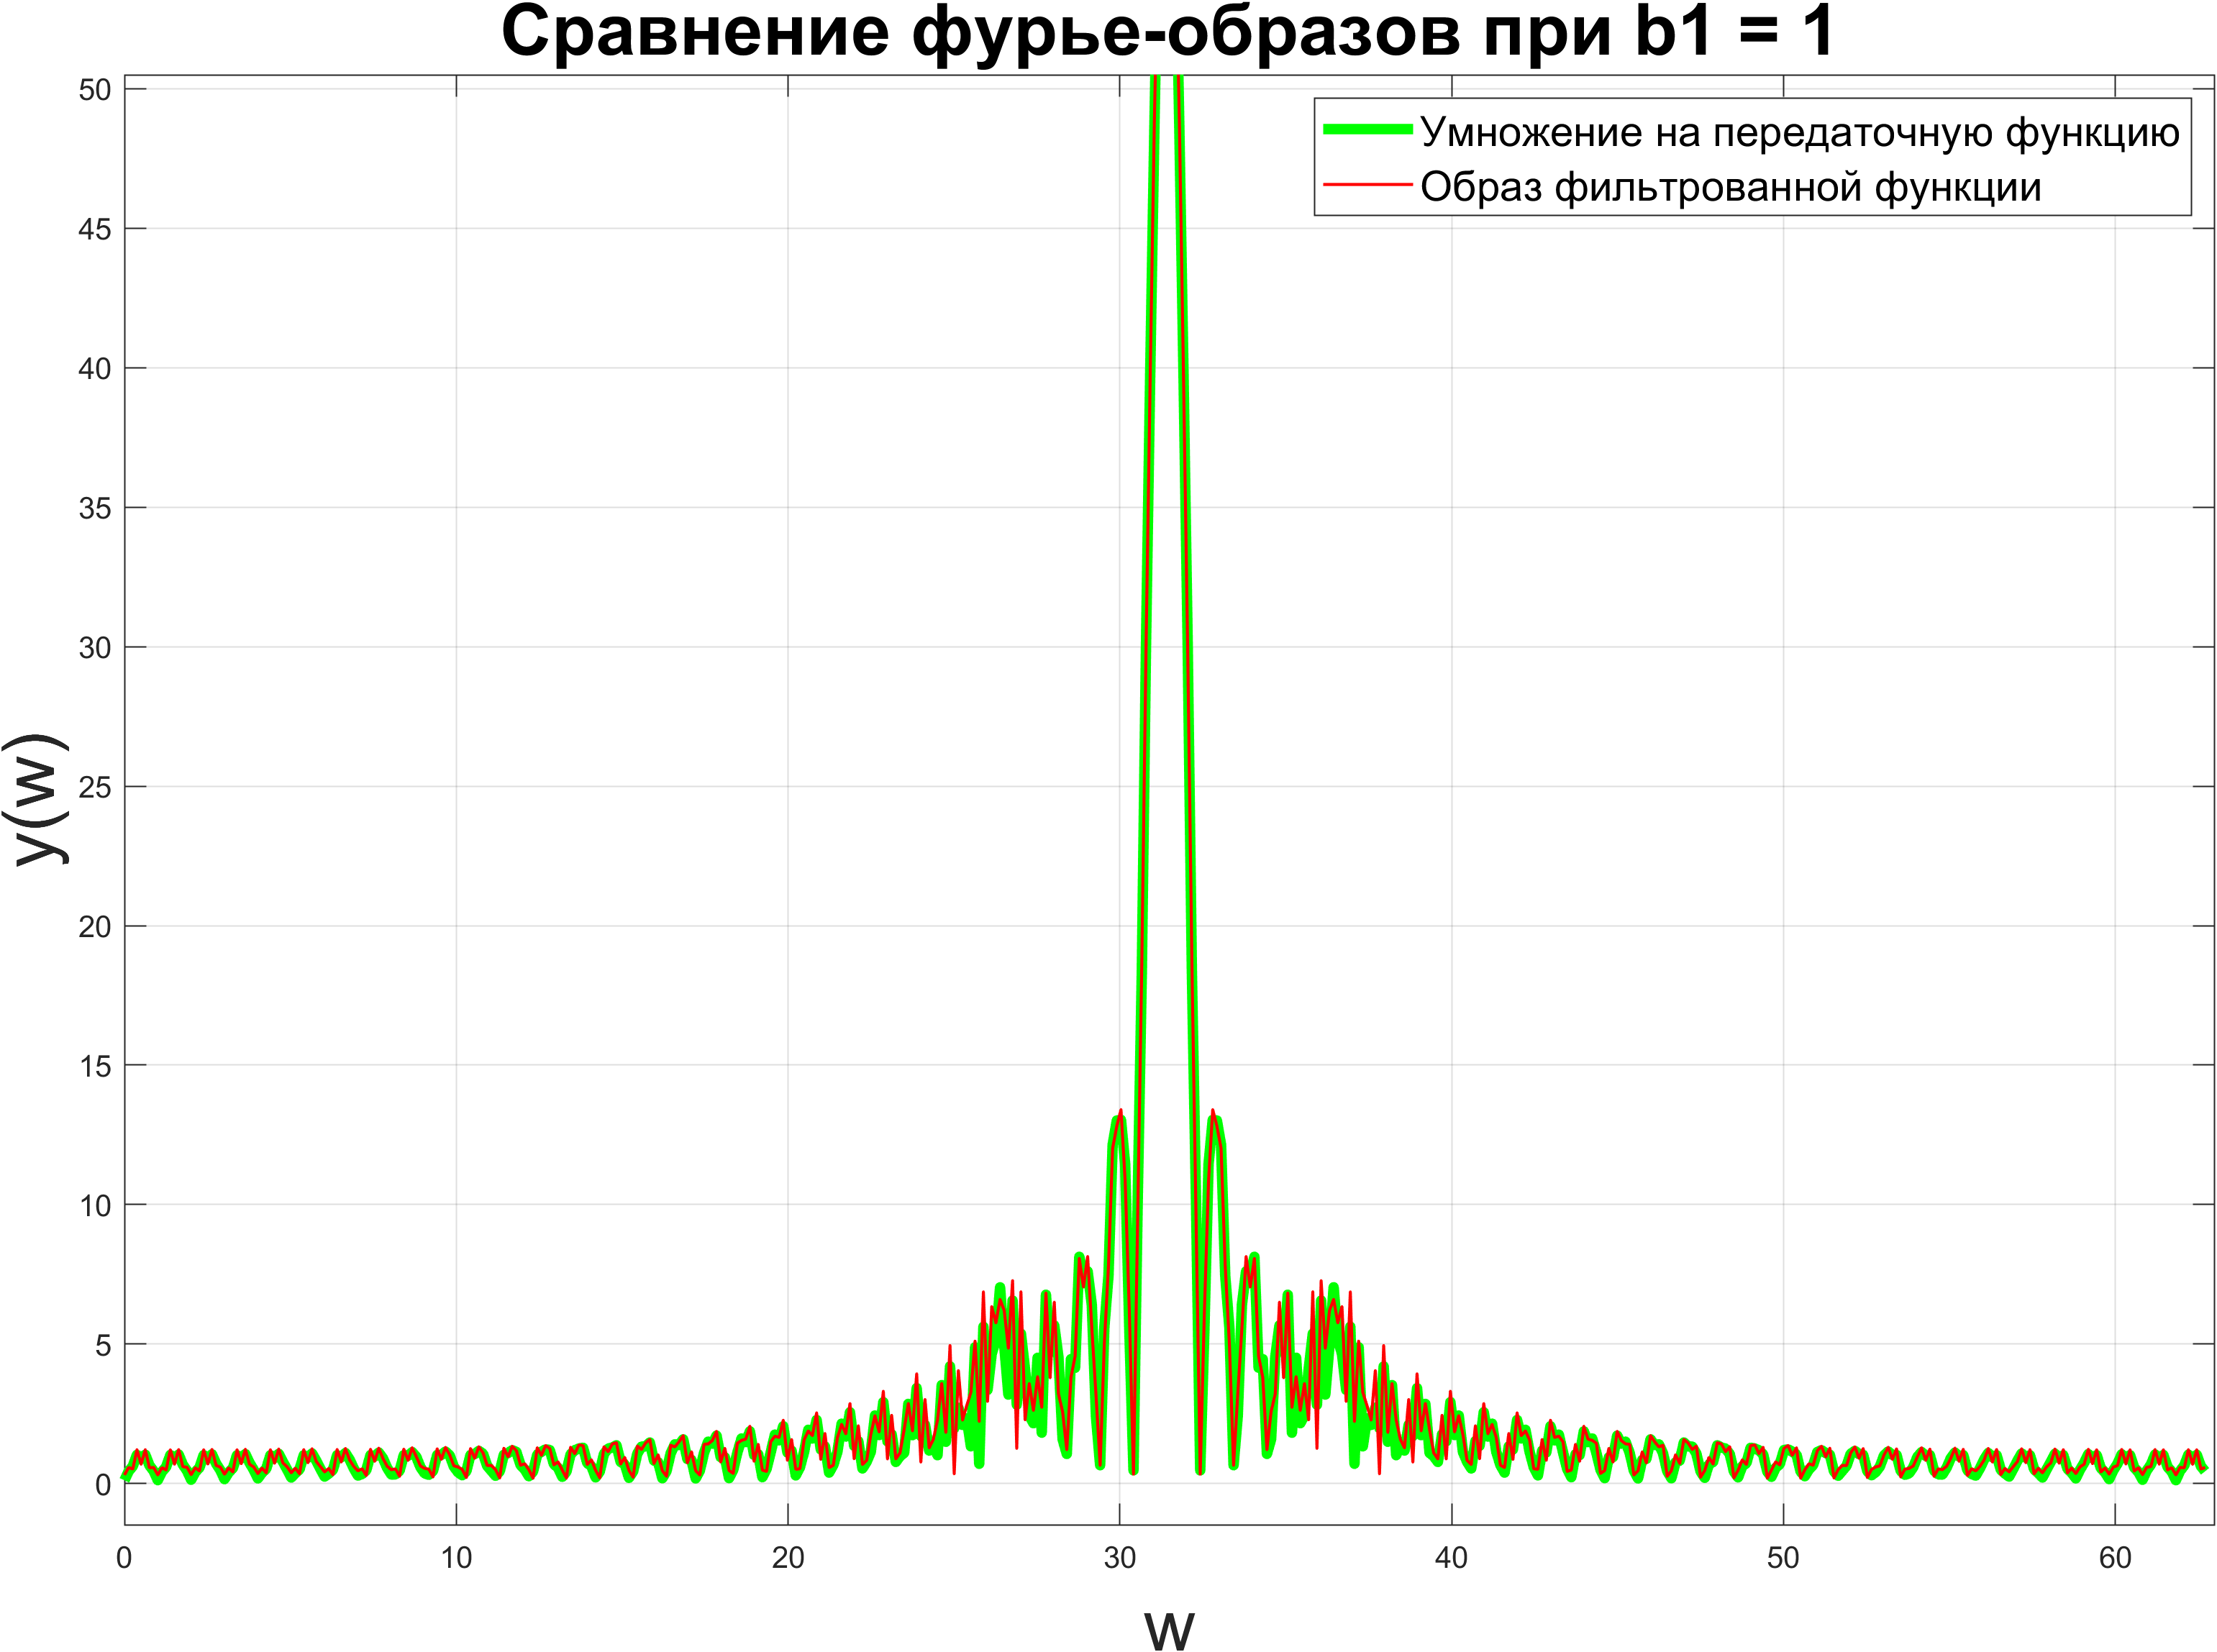
\includegraphics[width=0.85\textwidth, keepaspectratio]{images2/fur_imgs_w_b1_1.png}
    \caption{Фурье-образы при $b_1 = 1$}
\end{figure}
\begin{figure}[H]
    \centering
    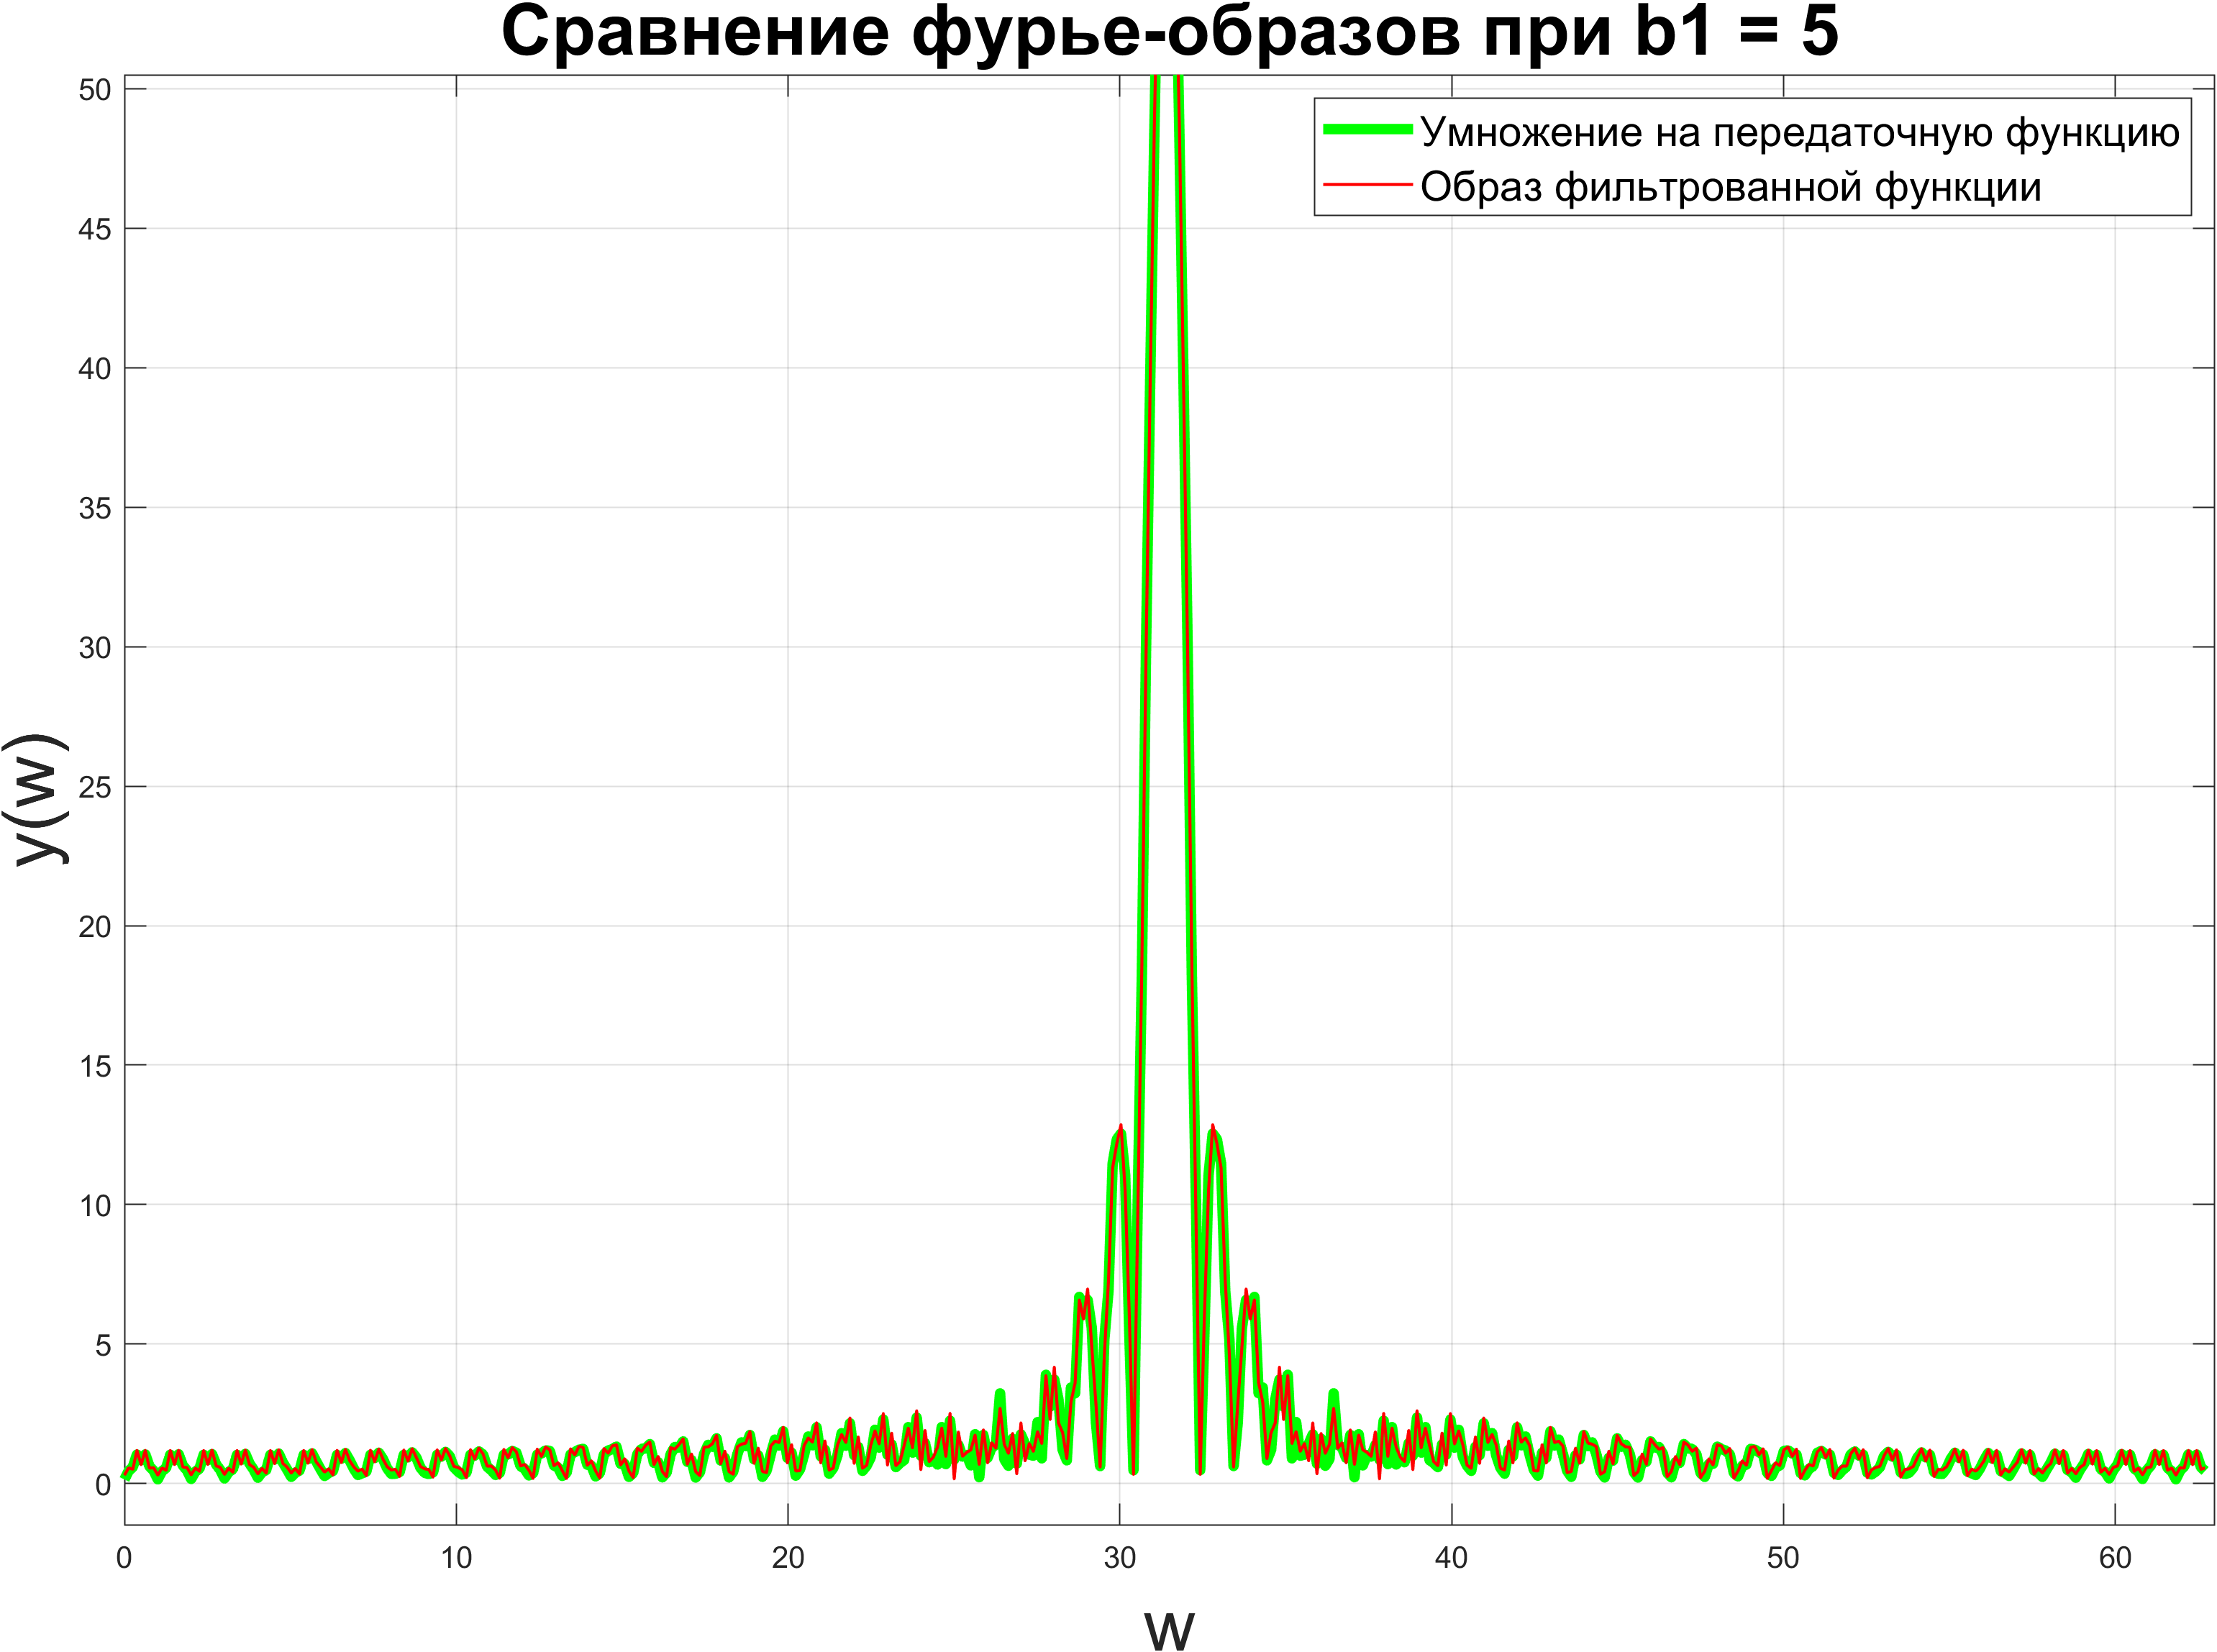
\includegraphics[width=0.85\textwidth, keepaspectratio]{images2/fur_imgs_w_b1_5.png}
    \caption{Фурье-образы при $b_1 = 5$}
\end{figure}
\newpage

\begin{figure}[H]
    \centering
    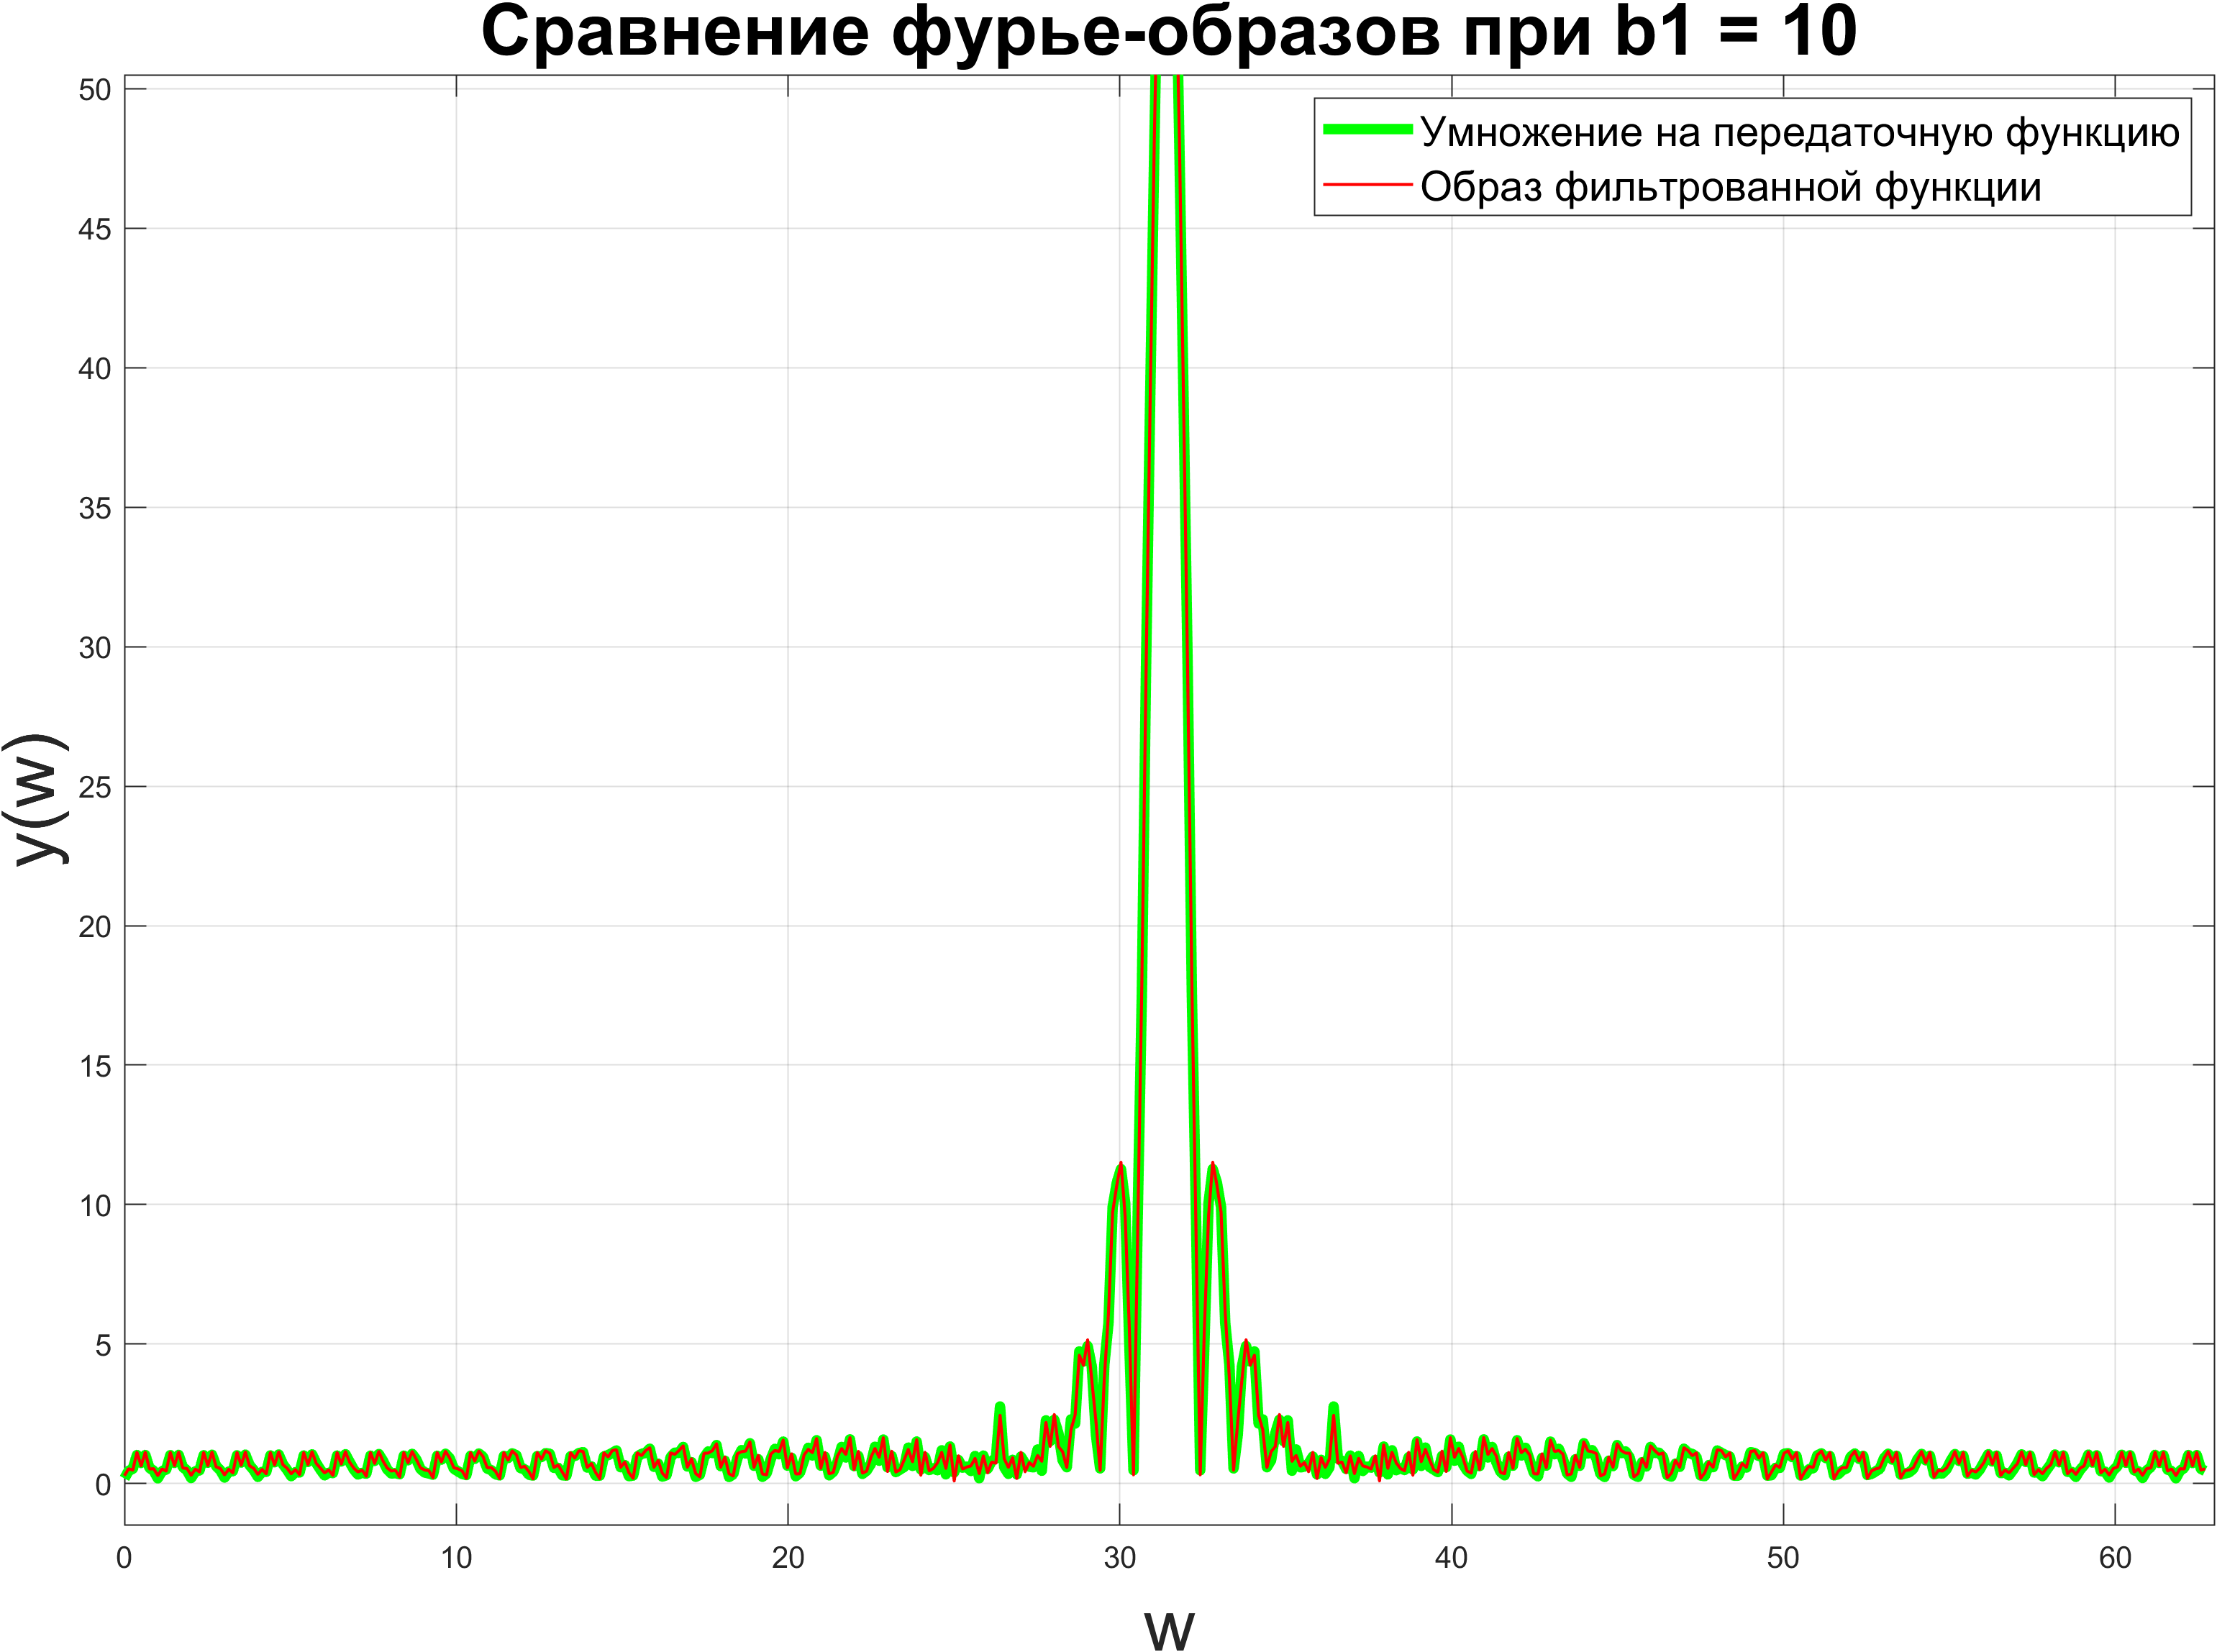
\includegraphics[width=0.90\textwidth, keepaspectratio]{images2/fur_imgs_w_b1_10.png}
    \caption{Фурье-образы при $b_1 = 10$}
\end{figure}
\begin{figure}[H]
    \centering
    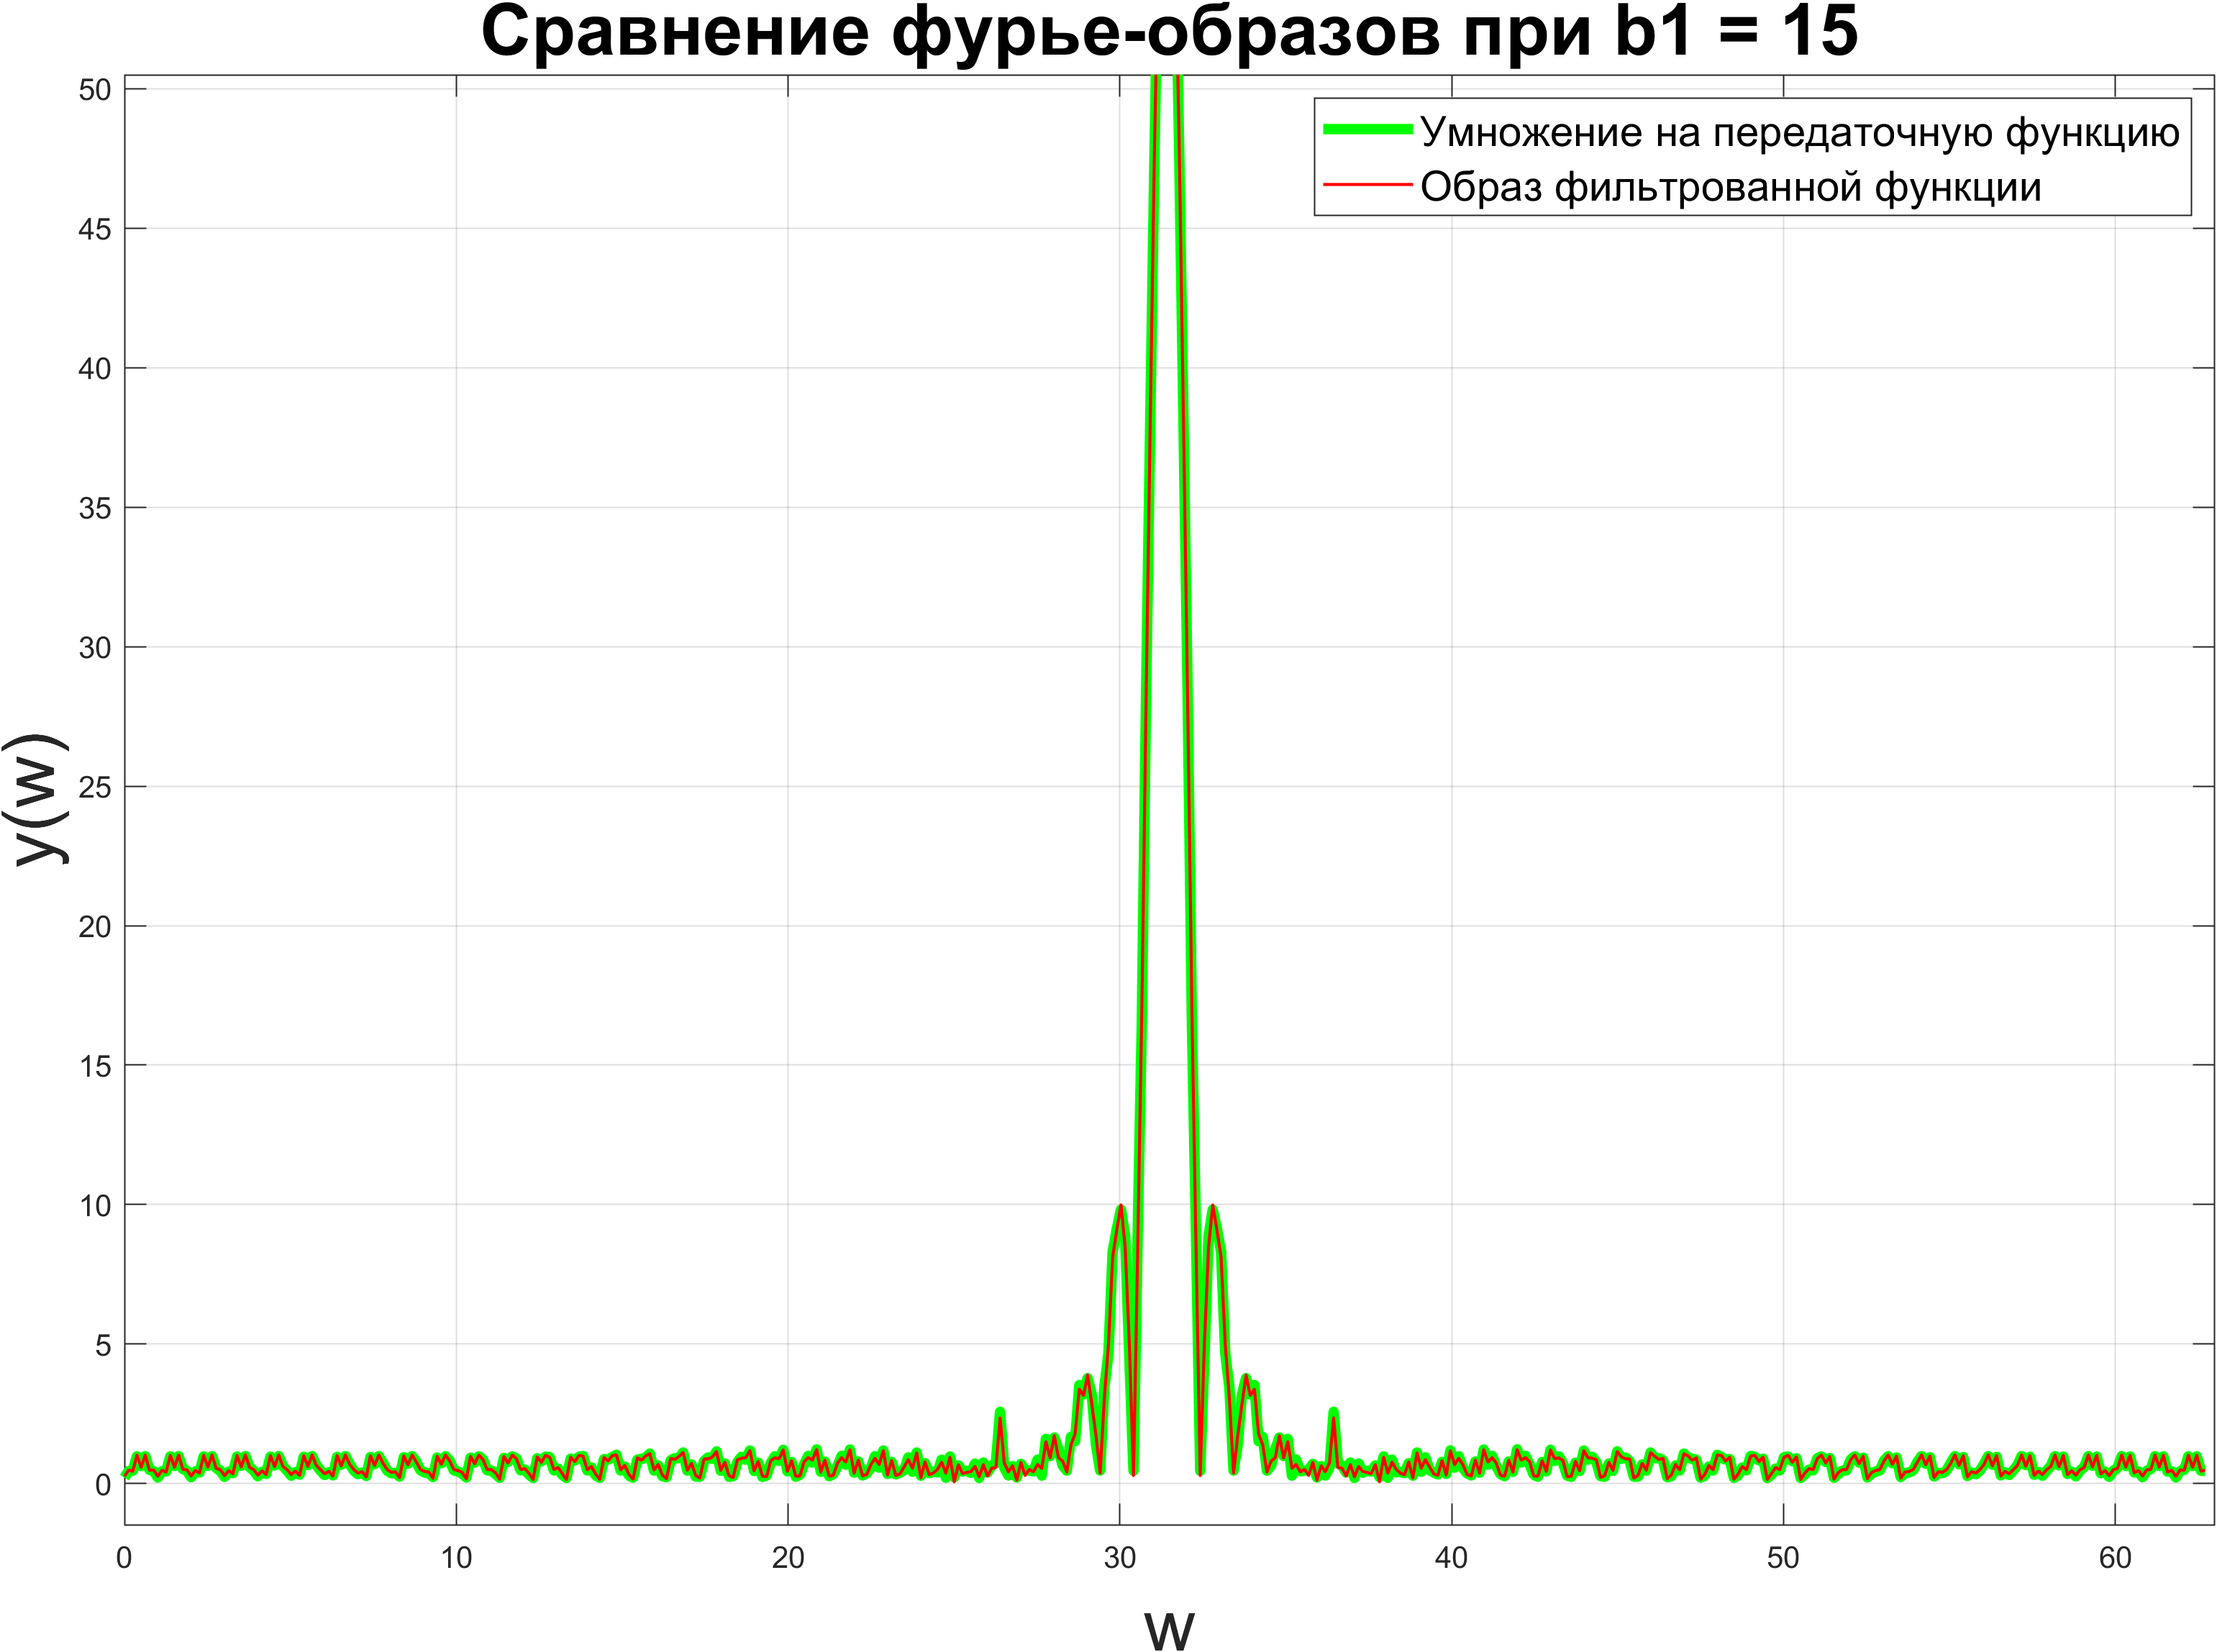
\includegraphics[width=0.90\textwidth, keepaspectratio]{images2/fur_imgs_w_b1_15.png}
    \caption{Фурье-образы при $b_1 = 15$}
\end{figure}
\newpage

\begin{figure}[H]
    \centering
    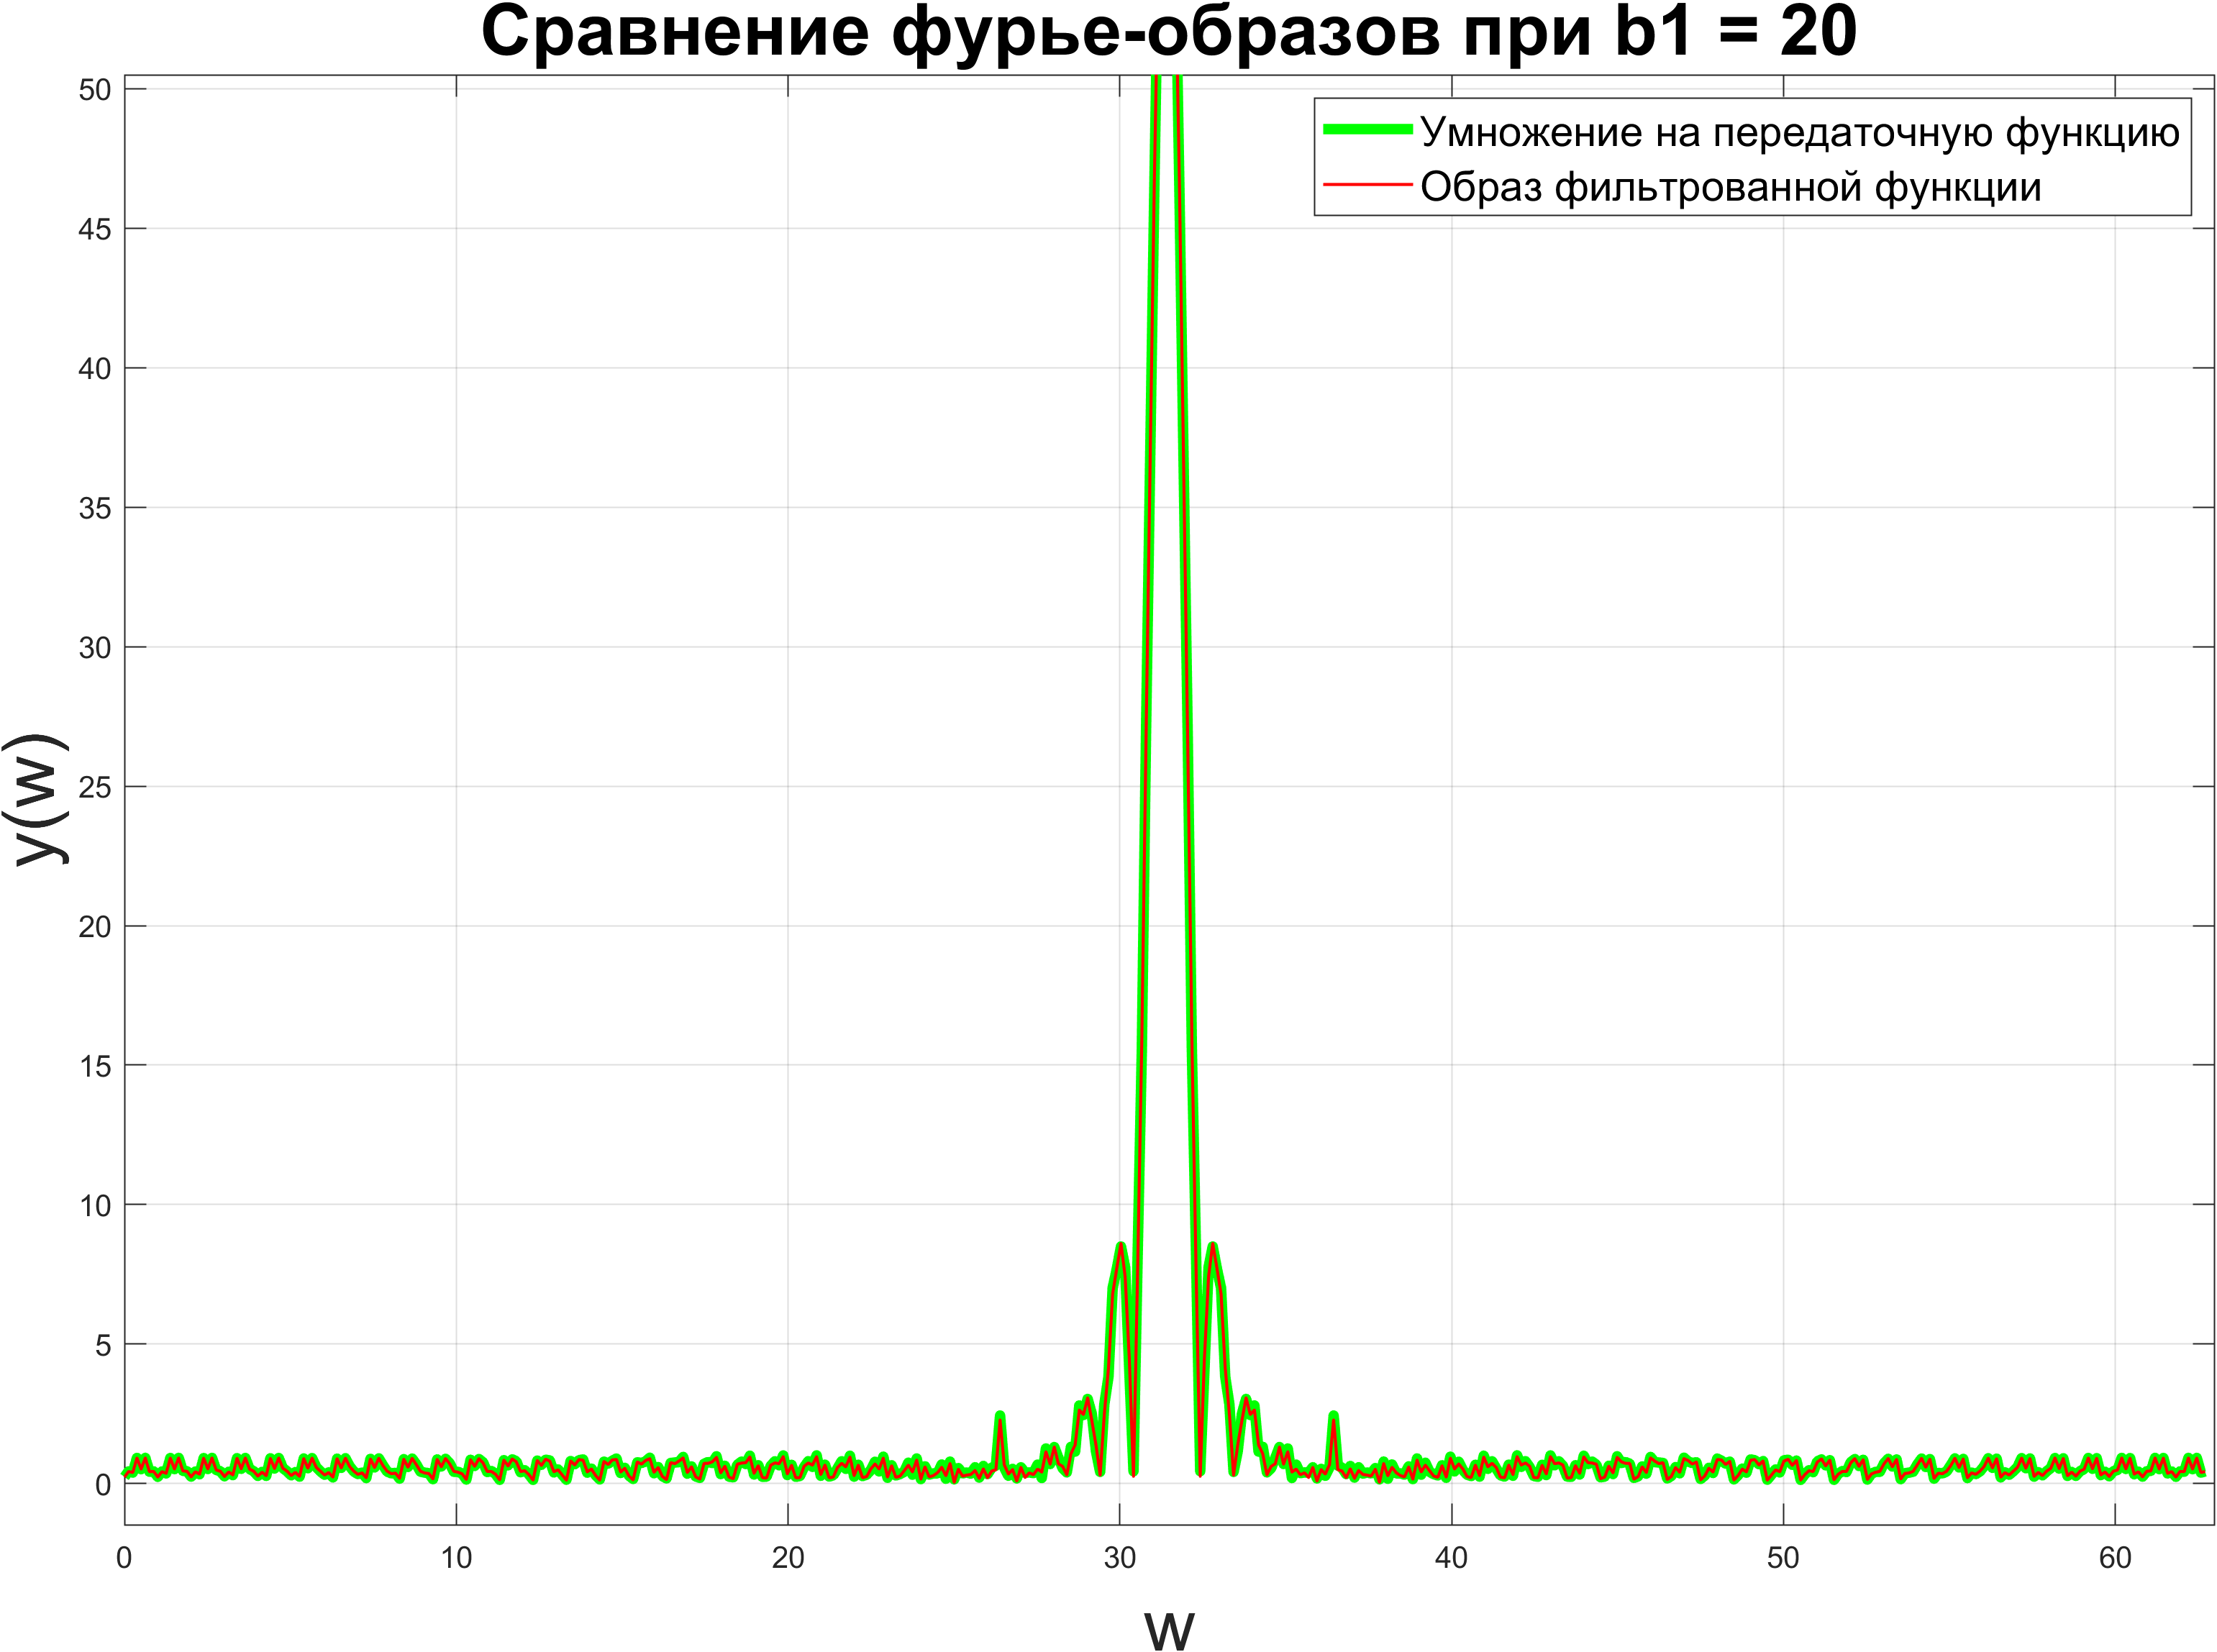
\includegraphics[width=0.90\textwidth, keepaspectratio]{images2/fur_imgs_w_b1_20.png}
    \caption{Фурье-образы при $b_1 = 20$}
\end{figure}
\begin{figure}[H]
    \centering
    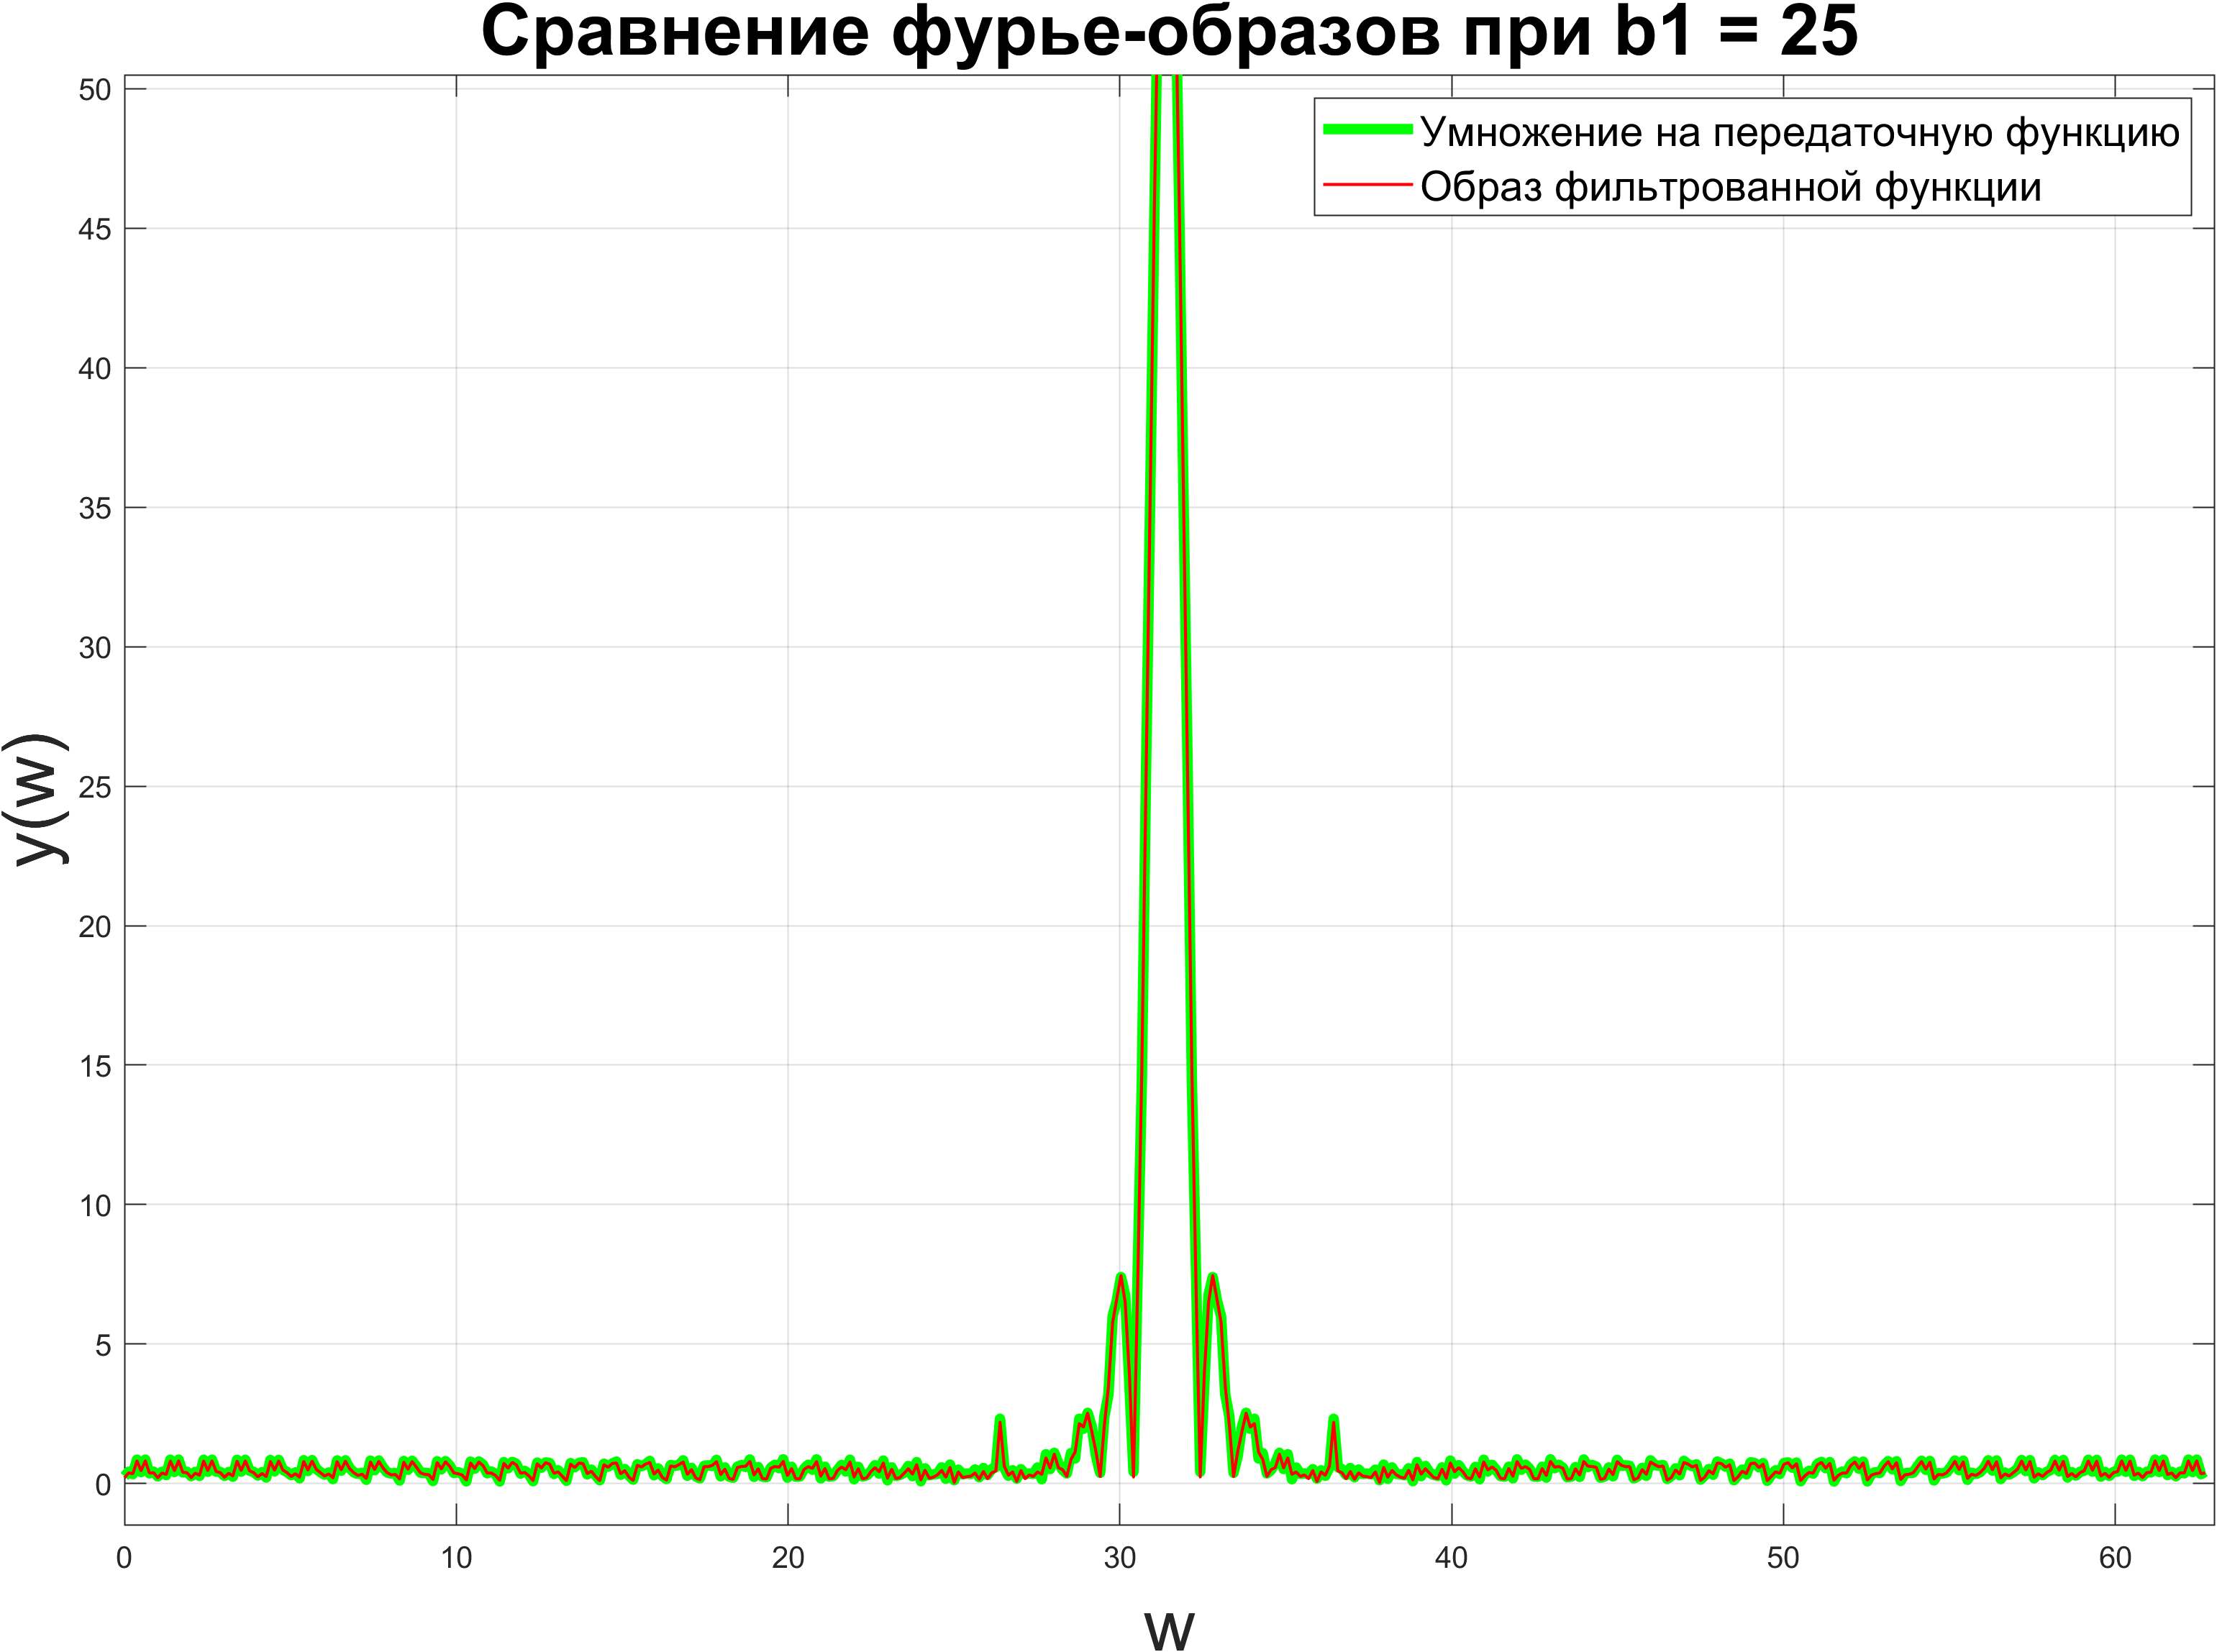
\includegraphics[width=0.90\textwidth, keepaspectratio]{images2/fur_imgs_w_b1_25.png}
    \caption{Фурье-образы при $b_1 = 25$}
\end{figure}

\subsection{ $d \neq \omega_0$ }
Также рассмотрим $d = 10$ и исследуем режекторный полосной фильтр в случае когда фильтруемая частота не совпадает с частотой шума:
Оставим прежними $\omega_0 = \sqrt{a_2} = \sqrt{b_2} = 5$:
\newline
Амплитудно-частотные характеристики:
\begin{figure}[H]
    \centering
    
\includegraphics[width=0.75\textwidth, keepaspectratio]{images3/filter_ach_b1_1.png}
    \caption{АЧХ при $b_1 = 1$}
\end{figure}
\begin{figure}[H]
    \centering
    
\includegraphics[width=0.75\textwidth, keepaspectratio]{images3/filter_ach_b1_5.png}
    \caption{АЧХ при $b_1 = 5$}
\end{figure}
\newpage

\begin{figure}[H]
    \centering
    
\includegraphics[width=0.92\textwidth, keepaspectratio]{images3/filter_ach_b1_10.png}
    \caption{АЧХ при $b_1 = 10$}
\end{figure}
\begin{figure}[H]
    \centering
    
\includegraphics[width=0.92\textwidth, keepaspectratio]{images3/filter_ach_b1_15.png}
    \caption{АЧХ при $b_1 = 15$}
\end{figure}
\newpage

\begin{figure}[H]
    \centering
    
\includegraphics[width=0.92\textwidth, keepaspectratio]{images3/filter_ach_b1_20.png}
    \caption{АЧХ при $b_1 = 20$}
\end{figure}
\begin{figure}[H]
    \centering
    
\includegraphics[width=0.92\textwidth, keepaspectratio]{images3/filter_ach_b1_25.png}
    \caption{АЧХ при $b_1 = 25$}
\end{figure}
\newpage

Демонстрация фильтрации сигнала:
\begin{figure}[H]
    \centering
    
\includegraphics[width=0.85\textwidth, keepaspectratio]{images3/filter_b1_1.png}
    \caption{Фильтрация при $b_1 = 1$}
\end{figure}
\begin{figure}[H]
    \centering
    
\includegraphics[width=0.85\textwidth, keepaspectratio]{images3/filter_b1_5.png}
    \caption{Фильтрация при $b_1 = 5$}
\end{figure}
\newpage

\begin{figure}[H]
    \centering
    
\includegraphics[width=0.92\textwidth, keepaspectratio]{images3/filter_b1_10.png}
    \caption{Фильтрация при $b_1 = 10$}
\end{figure}
\begin{figure}[H]
    \centering
    
\includegraphics[width=0.92\textwidth, keepaspectratio]{images3/filter_b1_15.png}
    \caption{Фильтрация при $b_1 = 15$}
\end{figure}
\newpage
\begin{figure}[H]
    \centering
    
\includegraphics[width=0.92\textwidth, keepaspectratio]{images3/filter_b1_20.png}
    \caption{Фильтрация при $b_1 = 20$}
\end{figure}
\begin{figure}[H]
    \centering
    
\includegraphics[width=0.92\textwidth, keepaspectratio]{images3/filter_b1_25.png}
    \caption{Фильтрация при $b_1 = 25$}
\end{figure}
\newpage

Сравнение фильтрованного сигнала и обратного Фурье-образа произведения частотной передаточной функции на Фурье-образ зашумленной функции:
\begin{figure}[H]
    \centering
    
\includegraphics[width=0.85\textwidth, keepaspectratio]{images3/filter_transf_b1_1.png}
    \caption{Сравнение методов при $b_1 = 1$}
\end{figure}
\begin{figure}[H]
    \centering
    
\includegraphics[width=0.85\textwidth, keepaspectratio]{images3/filter_transf_b1_5.png}
    \caption{Сравнение методов при $b_1 = 5$}
\end{figure}
\newpage
\begin{figure}[H]
    \centering
    
\includegraphics[width=0.92\textwidth, keepaspectratio]{images3/filter_transf_b1_10.png}
    \caption{Сравнение методов при $b_1 = 10$}
\end{figure}
\begin{figure}[H]
    \centering
    
\includegraphics[width=0.92\textwidth, keepaspectratio]{images3/filter_transf_b1_15.png}
    \caption{Сравнение методов при $b_1 = 15$}
\end{figure}
\newpage
\begin{figure}[H]
    \centering
    
\includegraphics[width=0.92\textwidth, keepaspectratio]{images3/filter_transf_b1_20.png}
    \caption{Сравнение методов при $b_1 = 20$}
\end{figure}
\begin{figure}[H]
    \centering
    
\includegraphics[width=0.92\textwidth, keepaspectratio]{images3/filter_transf_b1_25.png}
    \caption{Сравнение методов при $b_1 = 25$}
\end{figure}
\newpage

Модули Фурье-образов исходного, зашумленного и фильтрованного сигналов:
\begin{figure}[H]
    \centering
    
\includegraphics[width=0.85\textwidth, keepaspectratio]{images3/fur_imgs_g_b1_1.png}
    \caption{Фурье-образы двух методов при $b_1 = 1$}
\end{figure}
\begin{figure}[H]
    \centering
    
\includegraphics[width=0.85\textwidth, keepaspectratio]{images3/fur_imgs_g_b1_5.png}
    \caption{Фурье-образы двух методов при $b_1 = 5$}
\end{figure}
\newpage

\begin{figure}[H]
    \centering
    
\includegraphics[width=0.90\textwidth, keepaspectratio]{images3/fur_imgs_g_b1_10.png}
    \caption{Фурье-образы двух методов при $b_1 = 10$}
\end{figure}
\begin{figure}[H]
    \centering
    
\includegraphics[width=0.90\textwidth, keepaspectratio]{images3/fur_imgs_g_b1_15.png}
    \caption{Фурье-образы двух методов при $b_1 = 15$}
\end{figure}
\newpage

\begin{figure}[H]
    \centering
    
\includegraphics[width=0.90\textwidth, keepaspectratio]{images3/fur_imgs_g_b1_20.png}
    \caption{Фурье-образы двух методов при $b_1 = 20$}
\end{figure}
\begin{figure}[H]
    \centering
    
\includegraphics[width=0.90\textwidth, keepaspectratio]{images3/fur_imgs_g_b1_25.png}
    \caption{Фурье-образы двух методов при $b_1 = 25$}
\end{figure}
\newpage

Сравнение модулей Фурье-образа фильрованной функции и произведения передаточной функции на Фурье-образ зашумленной функции
\begin{figure}[H]
    \centering
    
\includegraphics[width=0.85\textwidth, keepaspectratio]{images3/fur_imgs_w_b1_1.png}
    \caption{Фурье-образы при $b_1 = 1$}
\end{figure}
\begin{figure}[H]
    \centering
    
\includegraphics[width=0.85\textwidth, keepaspectratio]{images3/fur_imgs_w_b1_5.png}
    \caption{Фурье-образы при $b_1 = 5$}
\end{figure}
\newpage

\begin{figure}[H]
    \centering
    
\includegraphics[width=0.90\textwidth, keepaspectratio]{images3/fur_imgs_w_b1_10.png}
    \caption{Фурье-образы при $b_1 = 10$}
\end{figure}
\begin{figure}[H]
    \centering
    
\includegraphics[width=0.90\textwidth, keepaspectratio]{images3/fur_imgs_w_b1_15.png}
    \caption{Фурье-образы при $b_1 = 15$}
\end{figure}
\newpage

\begin{figure}[H]
    \centering
    
\includegraphics[width=0.90\textwidth, keepaspectratio]{images3/fur_imgs_w_b1_20.png}
    \caption{Фурье-образы при $b_1 = 20$}
\end{figure}
\begin{figure}[H]
    \centering
    
\includegraphics[width=0.90\textwidth, keepaspectratio]{images3/fur_imgs_w_b1_25.png}
    \caption{Фурье-образы при $b_1 = 25$}
\end{figure}
\newpage
\subsection{Выводы}
Видим, что параметры $a_2 = b_2$ равны квадрату фильтруемой частоты $\omega_0$, параметр $d$ равен частоте добавленного шума, от параметра $b_1$ зависит насколько сильно уменьшаются частоты вблизи $\omega_0$: чем меньше $b_1$ тем меньший отрезок частот уменьшается значительно.
\newpage
\section{Сглаживание биржевых данных}
\subsection{Описание задания}
В этом задании мы применили динамический фильтр низких частот 1 порядка (использовался в задании 1), для сглаживания графика акций сбербанка в период с $03.01.2022$ по $21.04.2026$.
\newline
Так как исходные данные содержали пропущенные дни, а функция lsim в Matlab применяется к равномерному массиву времени мы продлилили пропуски внутри данных линейно между началом пропущенного промежутка и концом пропущенного промежутка. 
\newline
Так как функция lsim строит график от нуля, мы вычли из массива стоимостей стоимость в первый рассматриваемый день, провели сглаживание полученного массива, а затем добавили стоимость в первый день обратно. 
\newline
Сглаживание производилось для значений параметра $T = 1, T = 7, T = 30, T = 365$ дней.

\newpage
\subsection{Графики}
\begin{figure}[H]
    \centering
    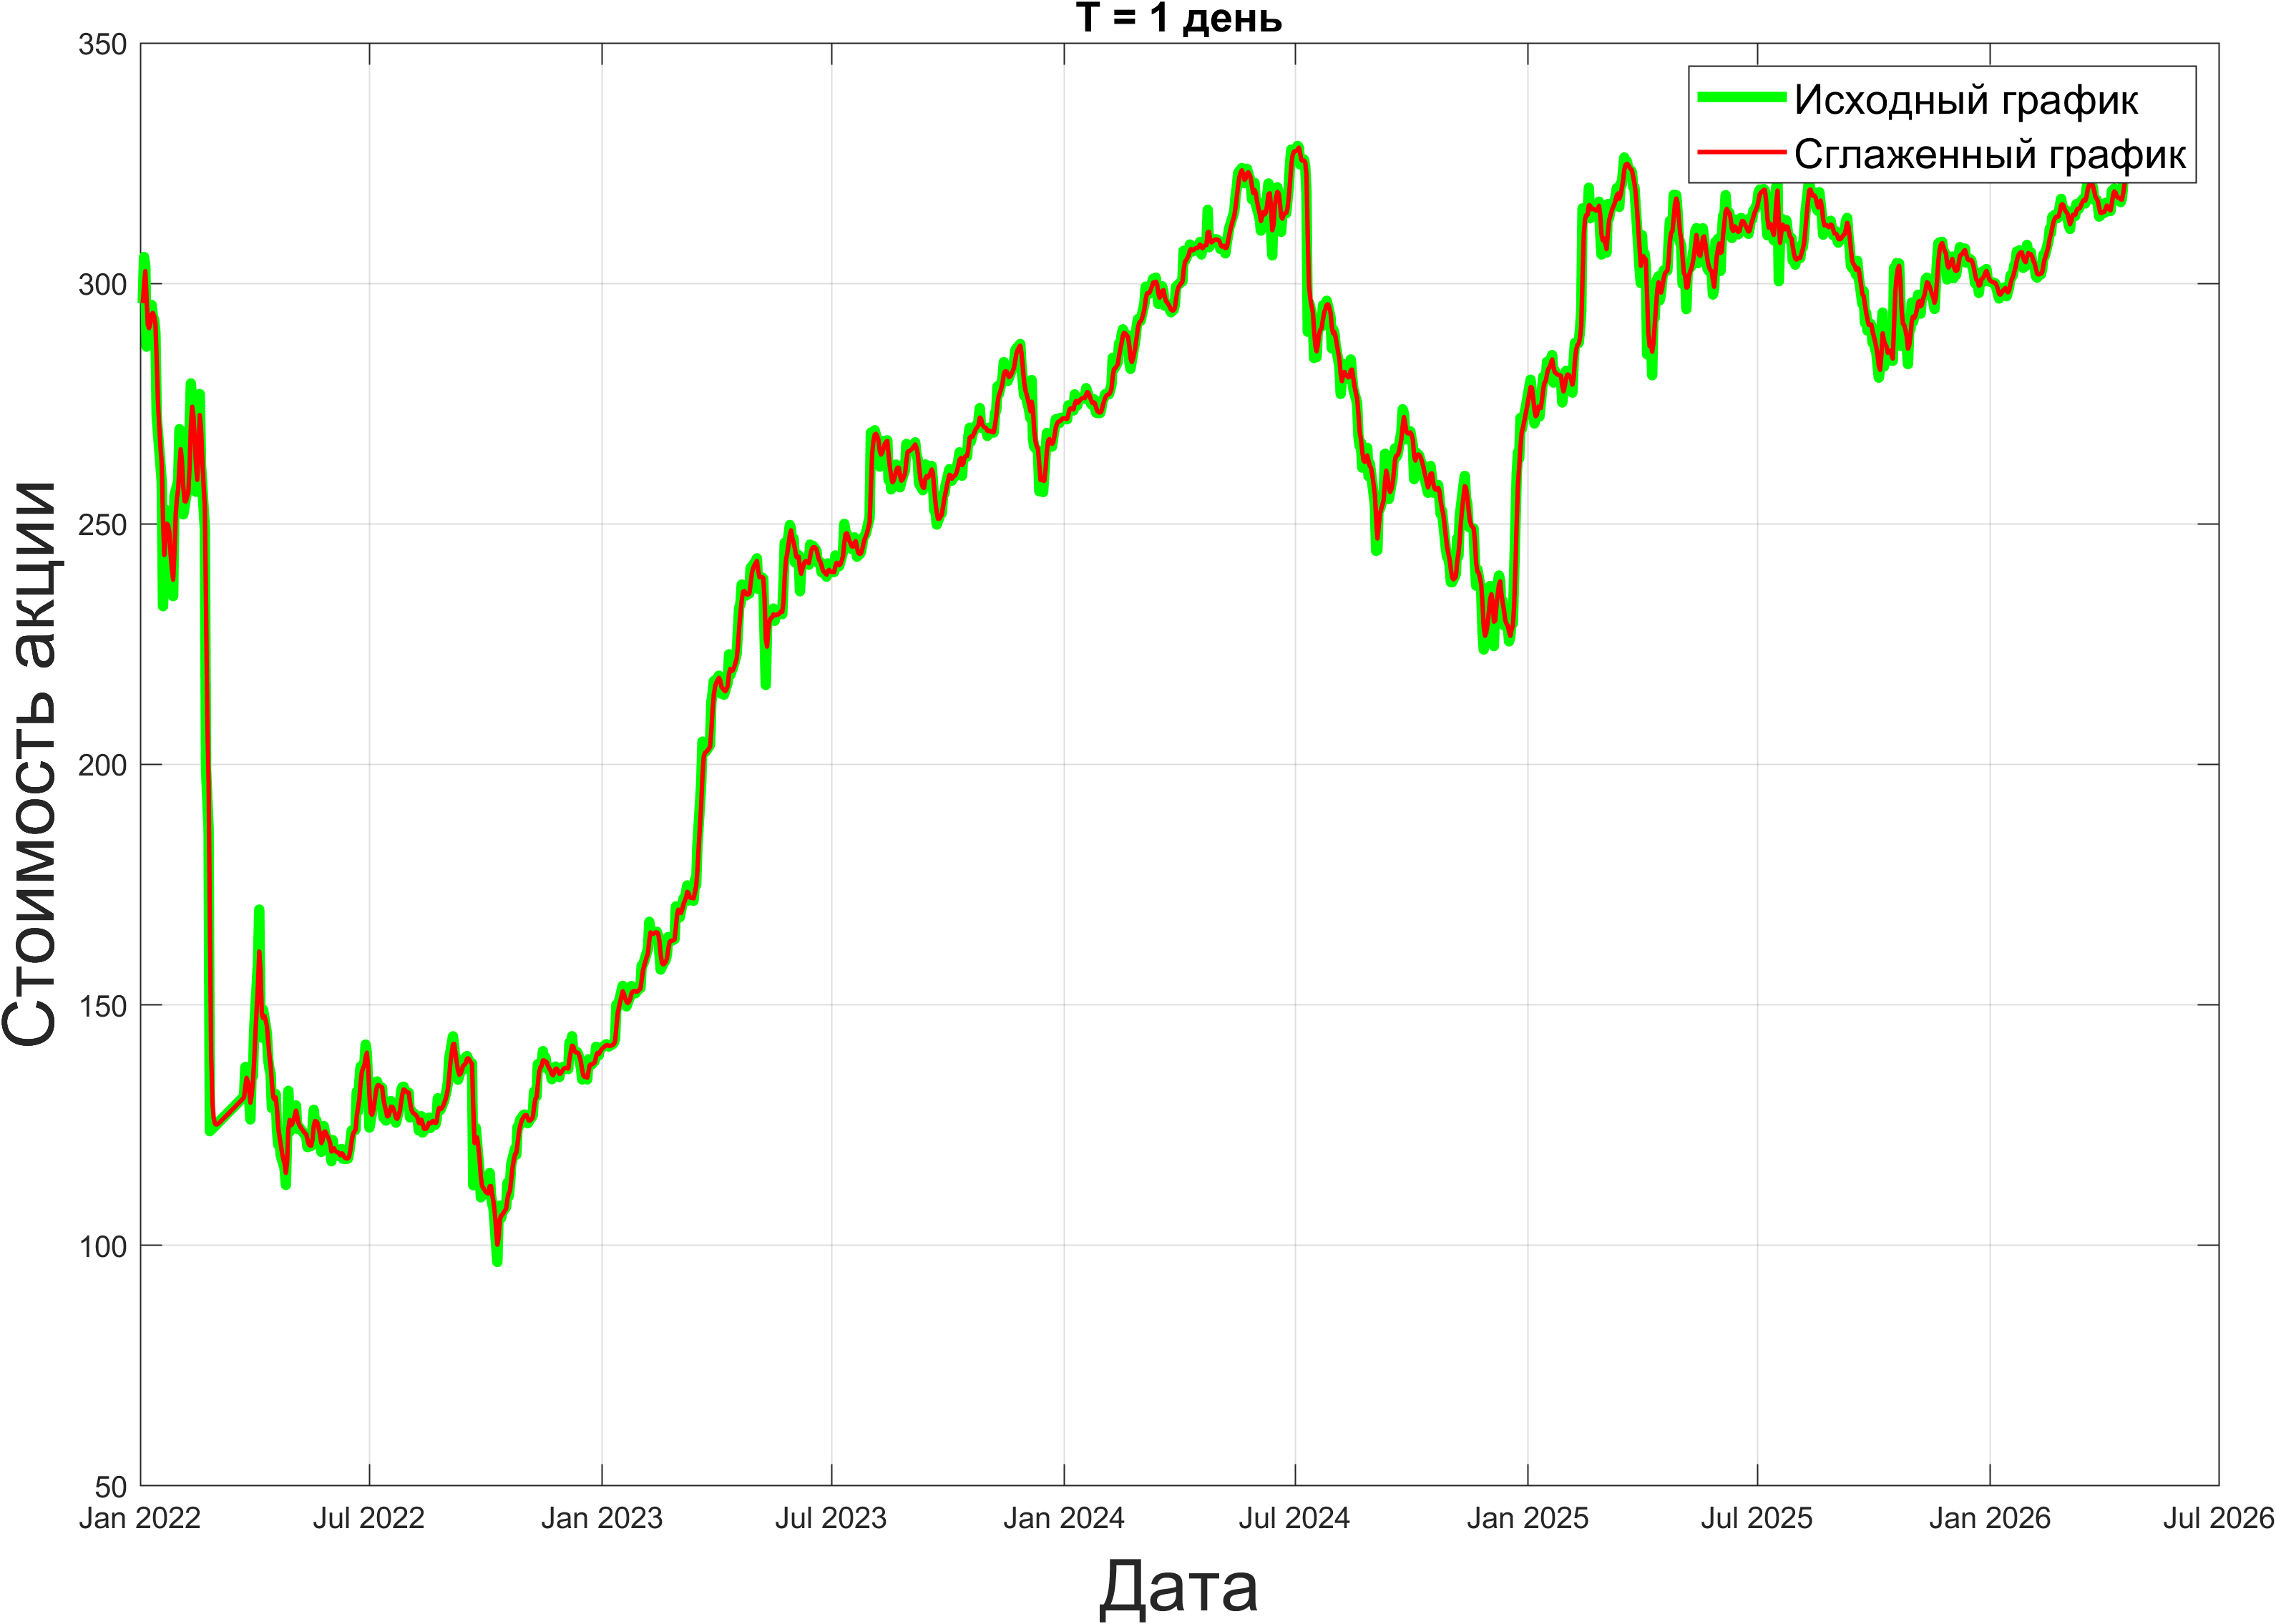
\includegraphics[width=0.90\textwidth, keepaspectratio]{images4/task3_1_1.png}
    \caption{Сглаживание, $T = 1$ день, все время}
\end{figure}
\begin{figure}[H]
    \centering
    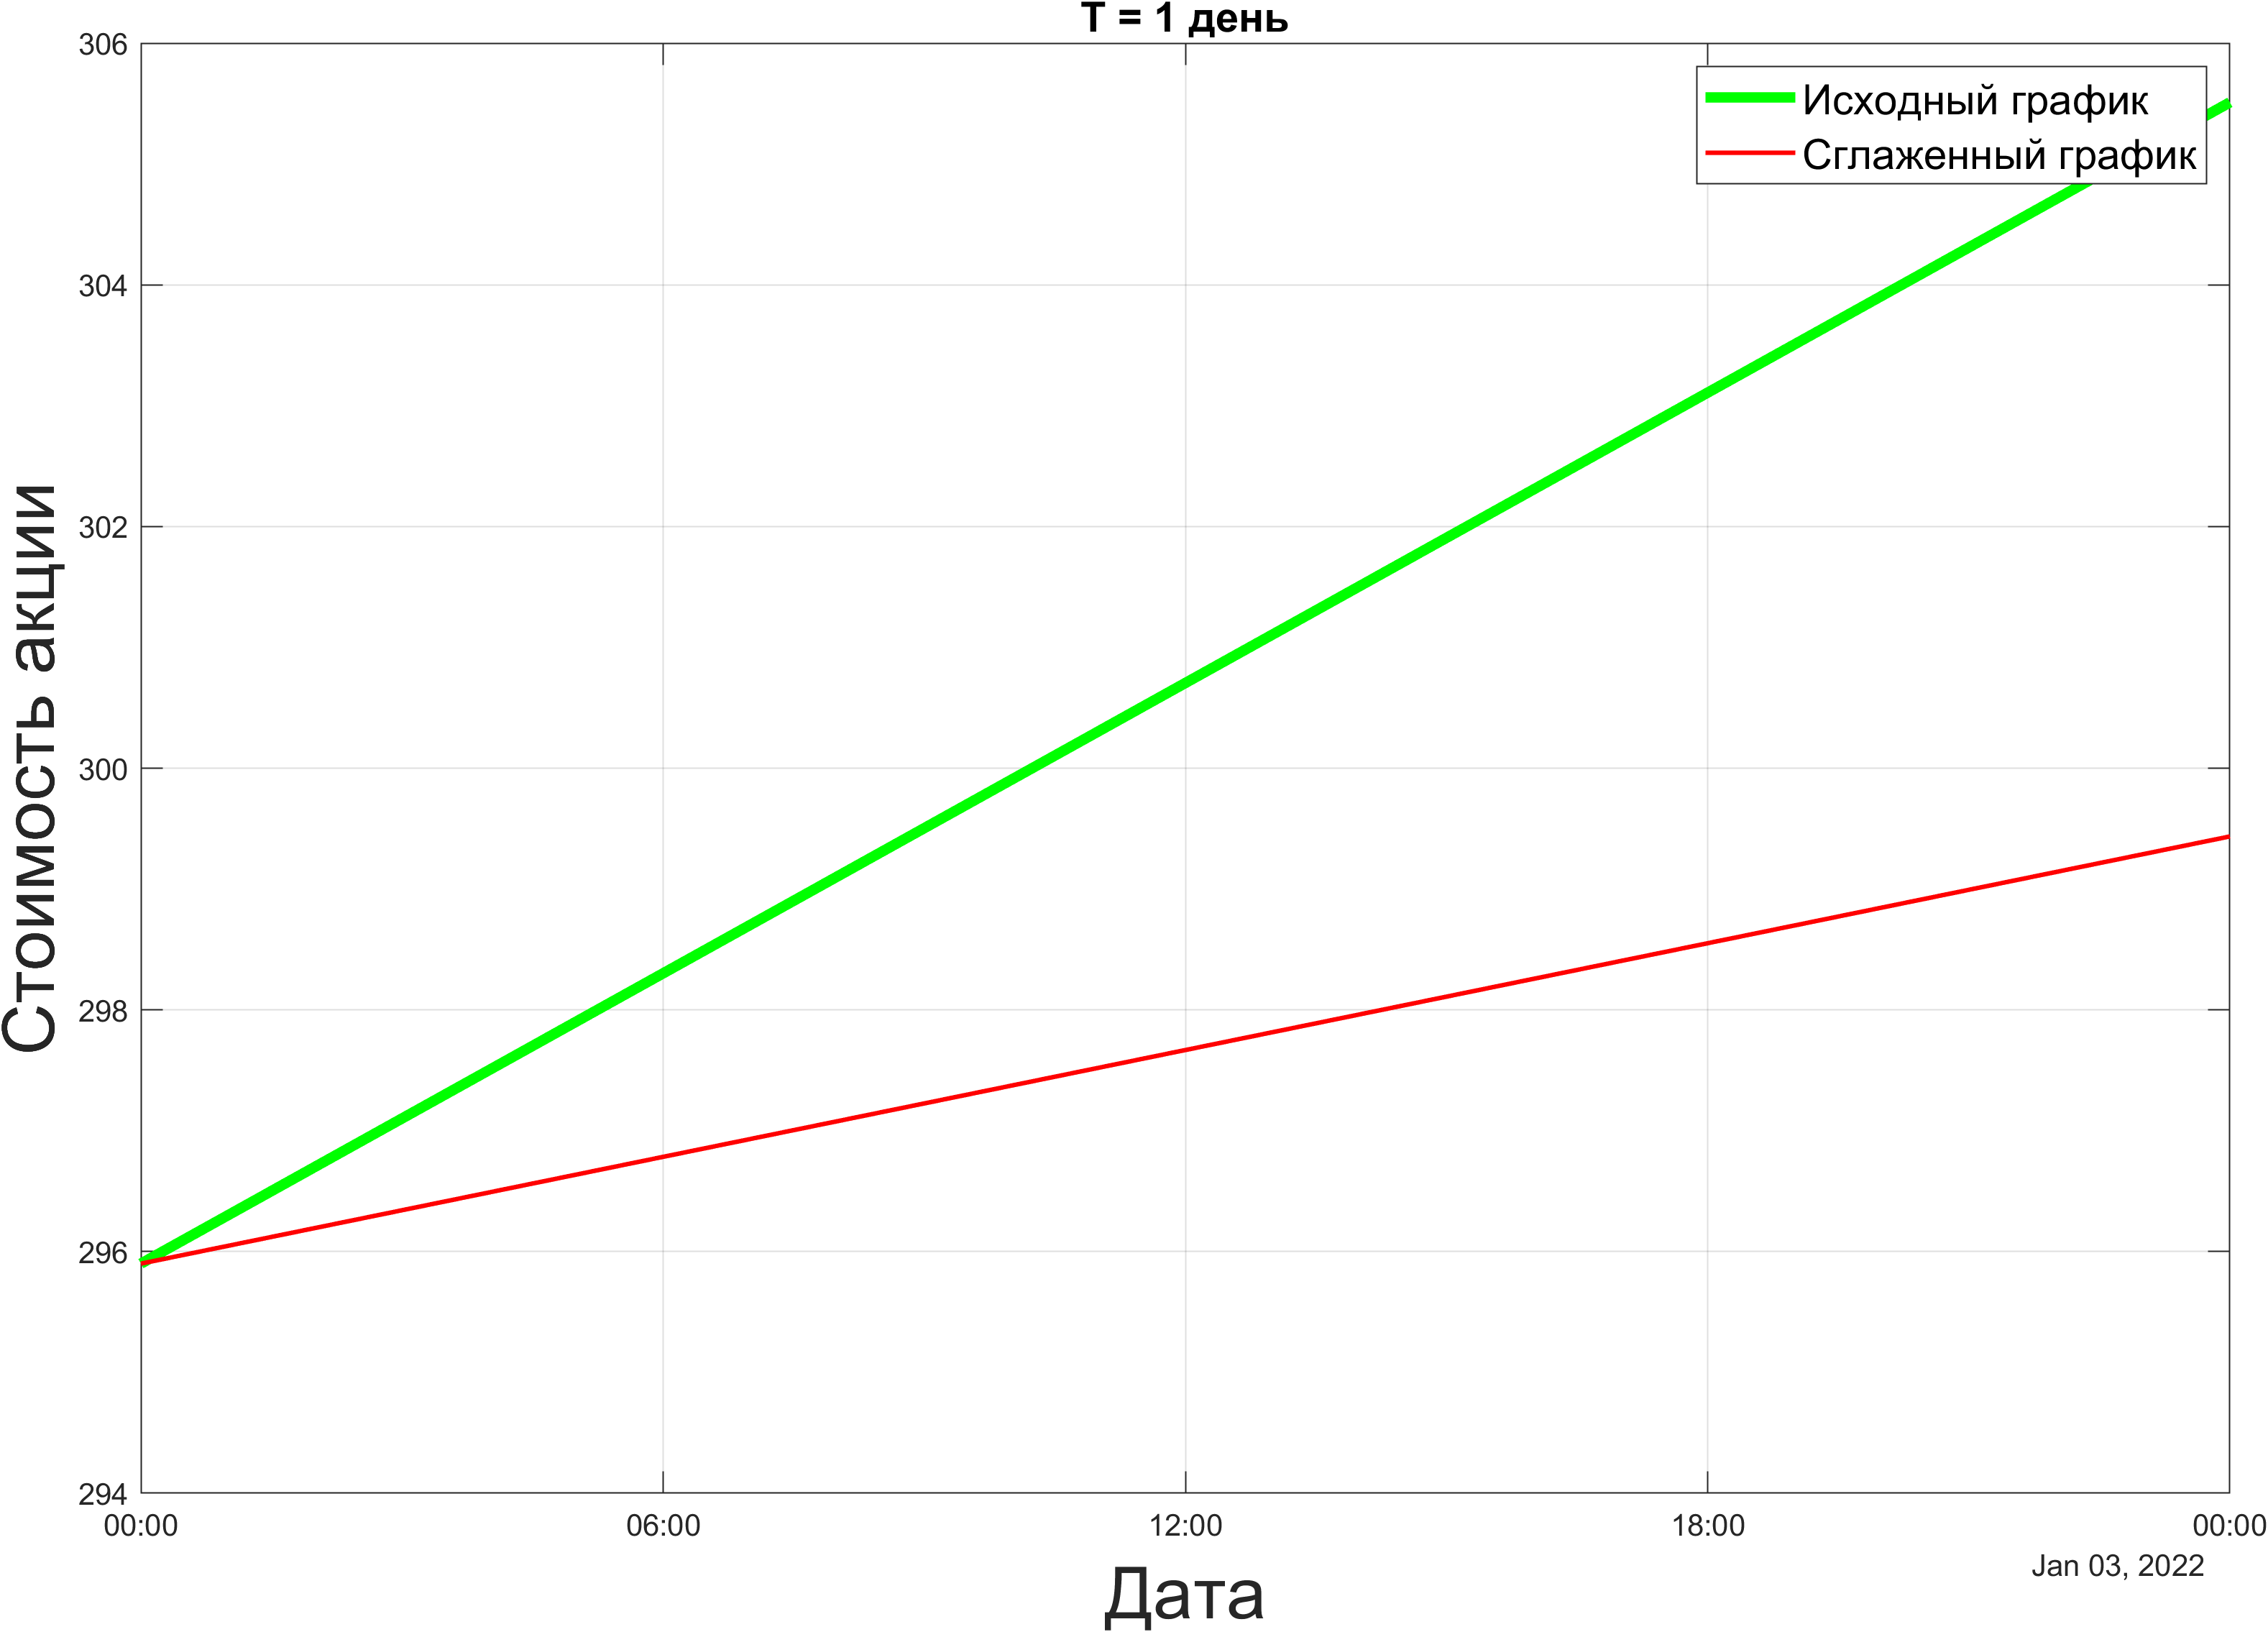
\includegraphics[width=0.90\textwidth, keepaspectratio]{images4/task3_1_2.png}
    \caption{Сглаживание, $T = 1$ день, период времени $T$}
\end{figure}
\newpage
\begin{figure}[H]
    \centering
    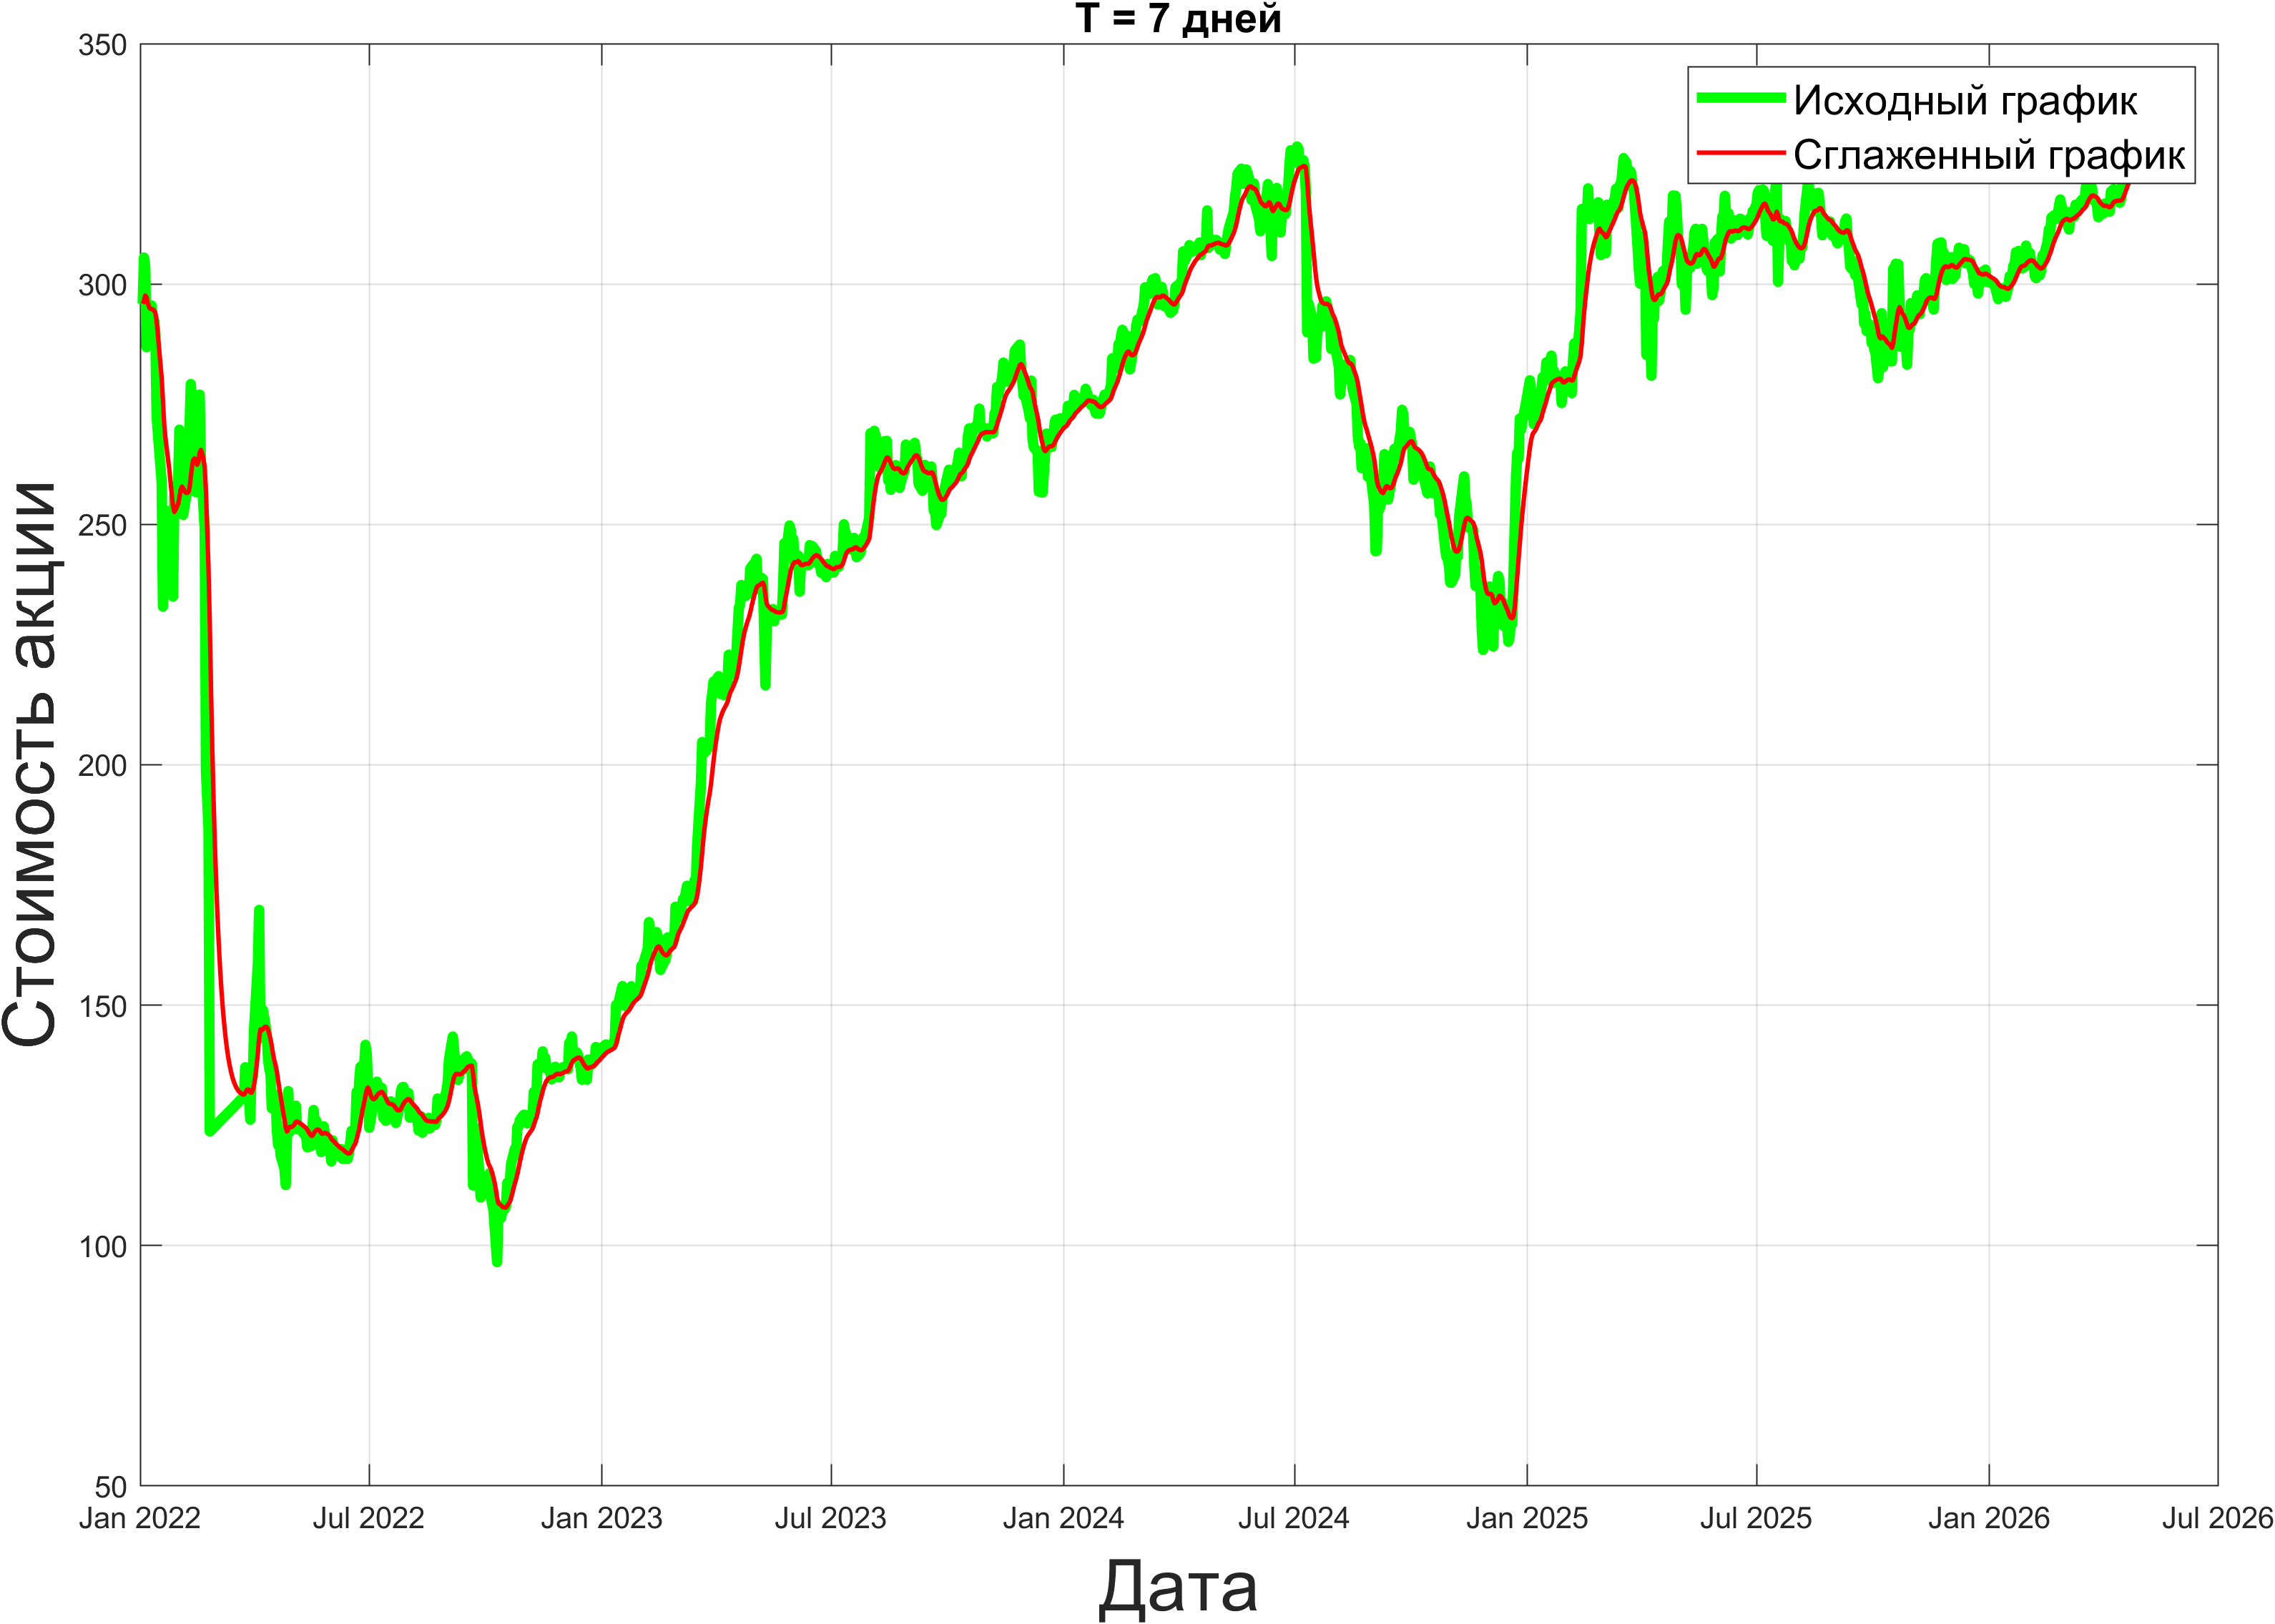
\includegraphics[width=0.90\textwidth, keepaspectratio]{images4/task3_7_1.png}
    \caption{Сглаживание, $T = 7$ дней, все время}
\end{figure}
\begin{figure}[H]
    \centering
    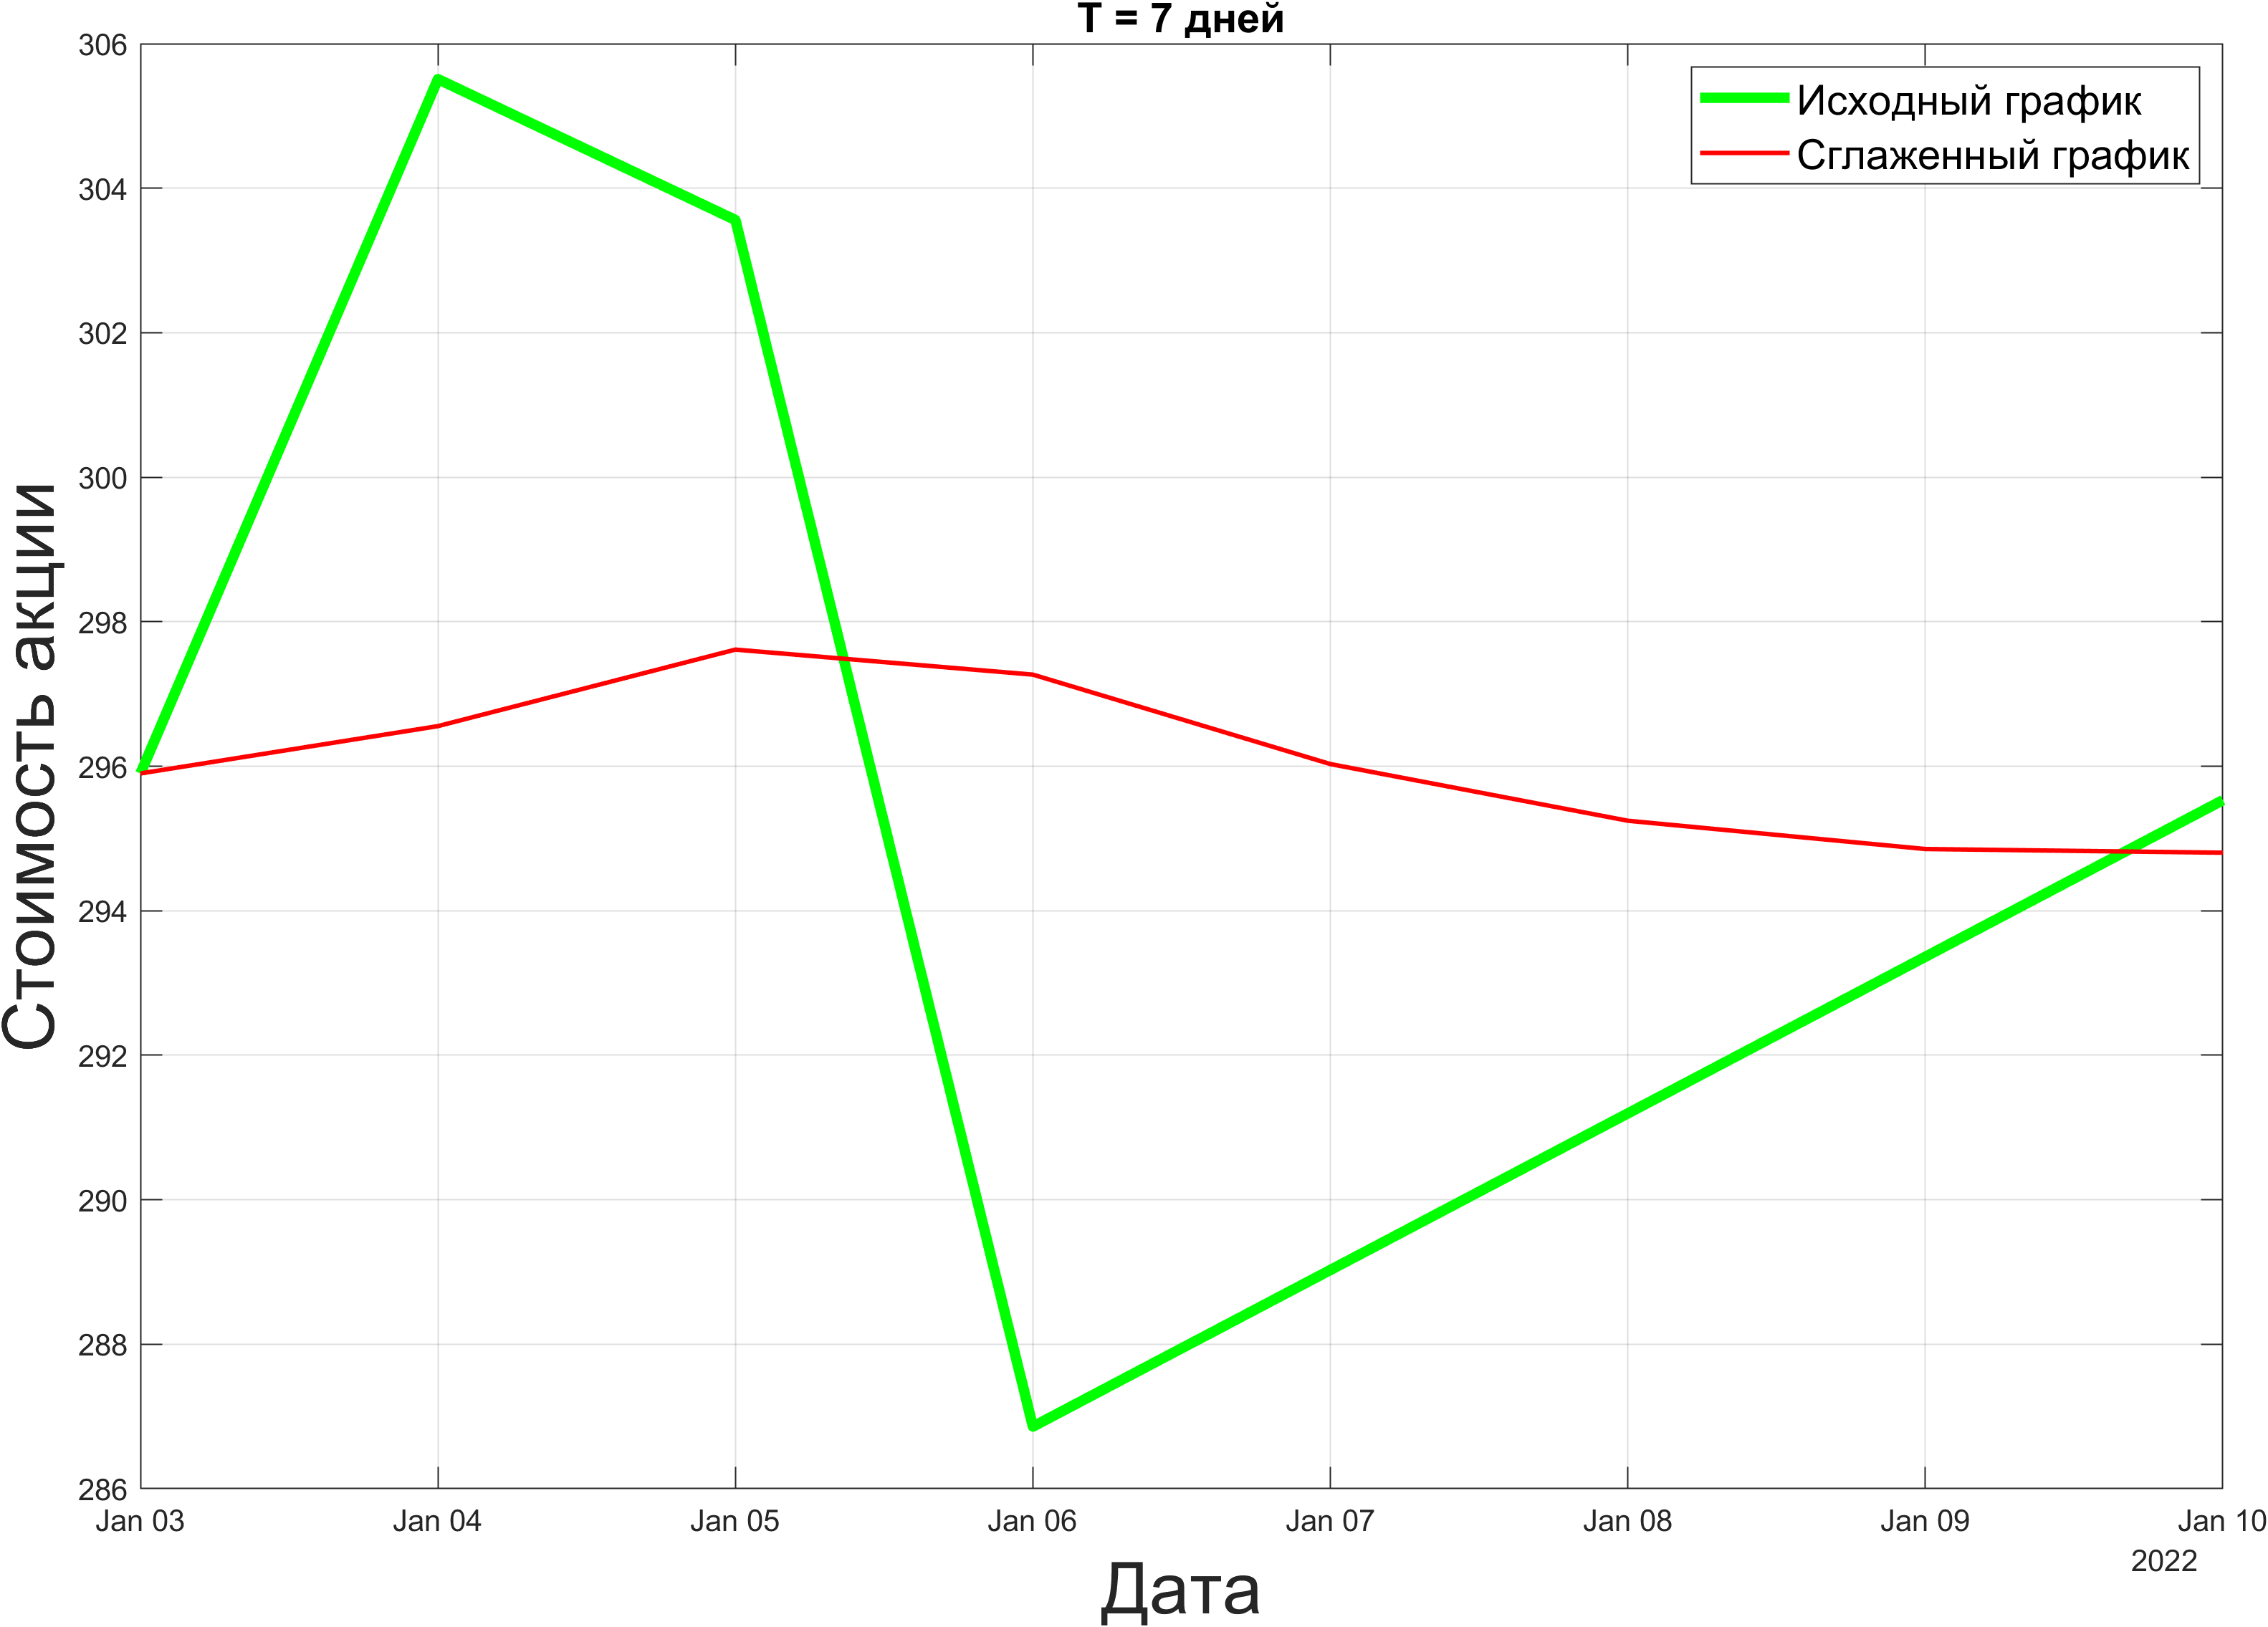
\includegraphics[width=0.90\textwidth, keepaspectratio]{images4/task3_7_2.png}
    \caption{Сглаживание, $T = 7$ дней, период времени $T$}
\end{figure}
\newpage
\begin{figure}[H]
    \centering
    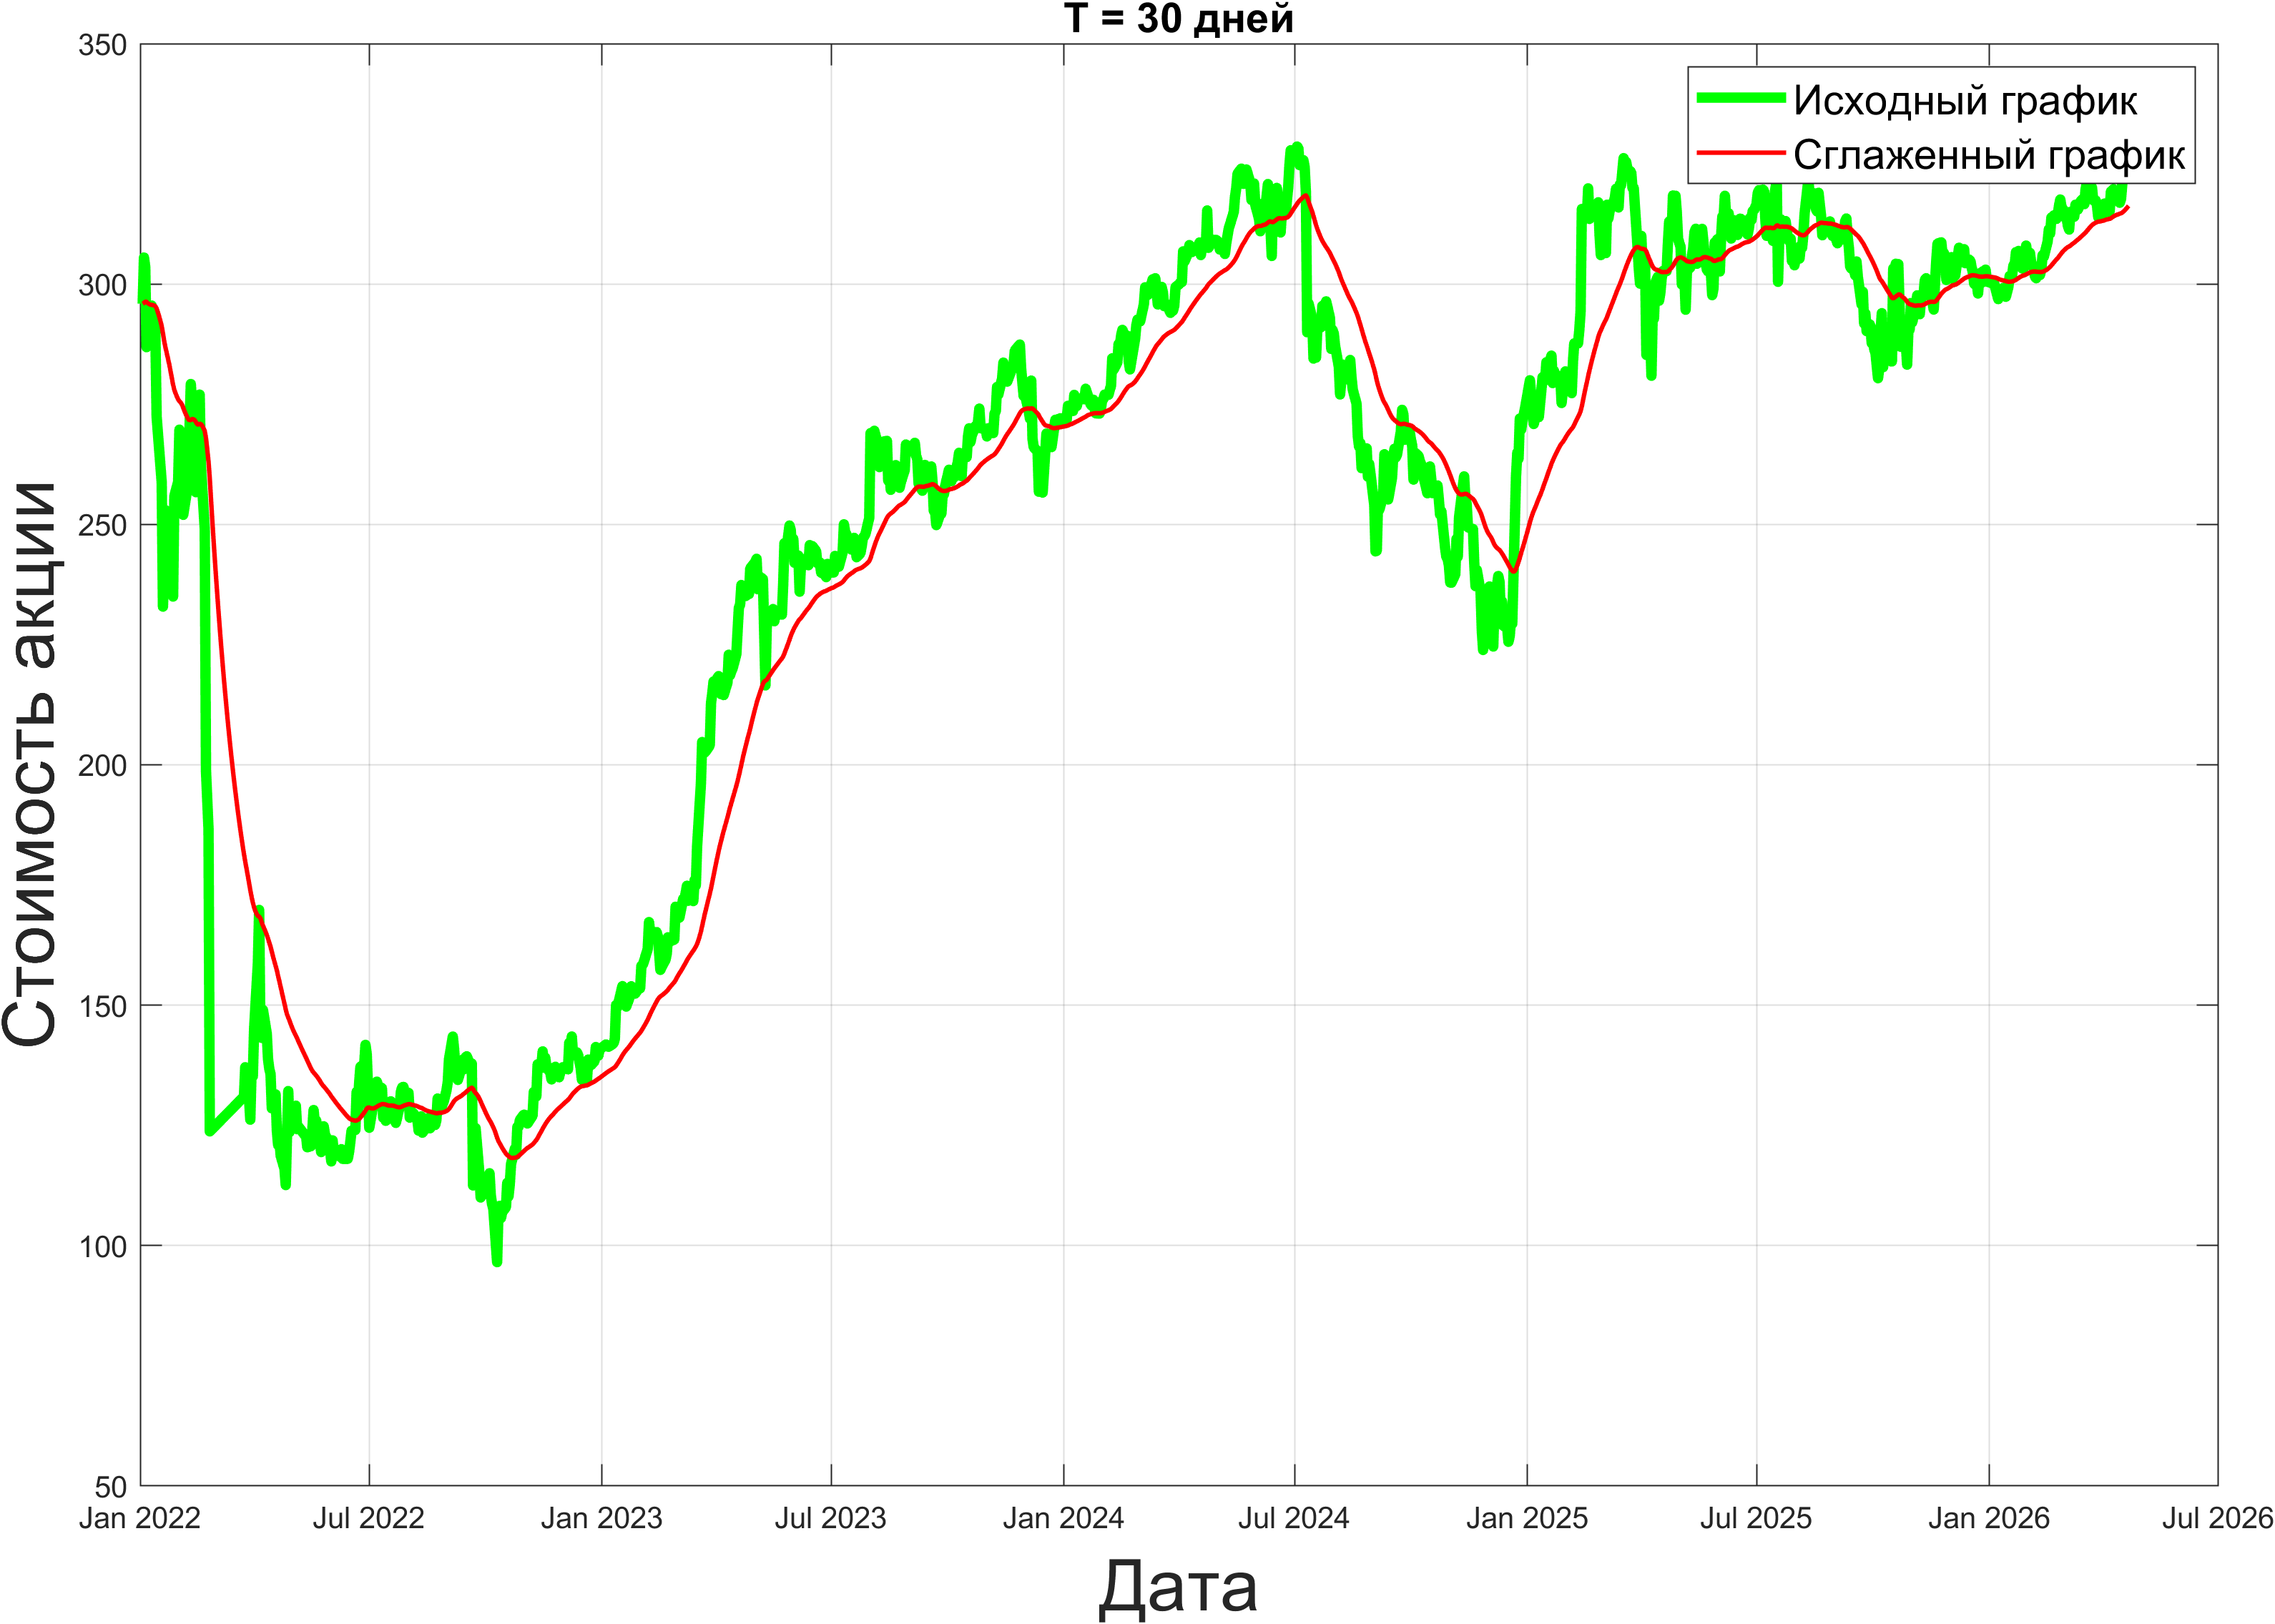
\includegraphics[width=0.90\textwidth, keepaspectratio]{images4/task3_30_1.png}
    \caption{Сглаживание, $T = 30$ дней, все время}
\end{figure}
\begin{figure}[H]
    \centering
    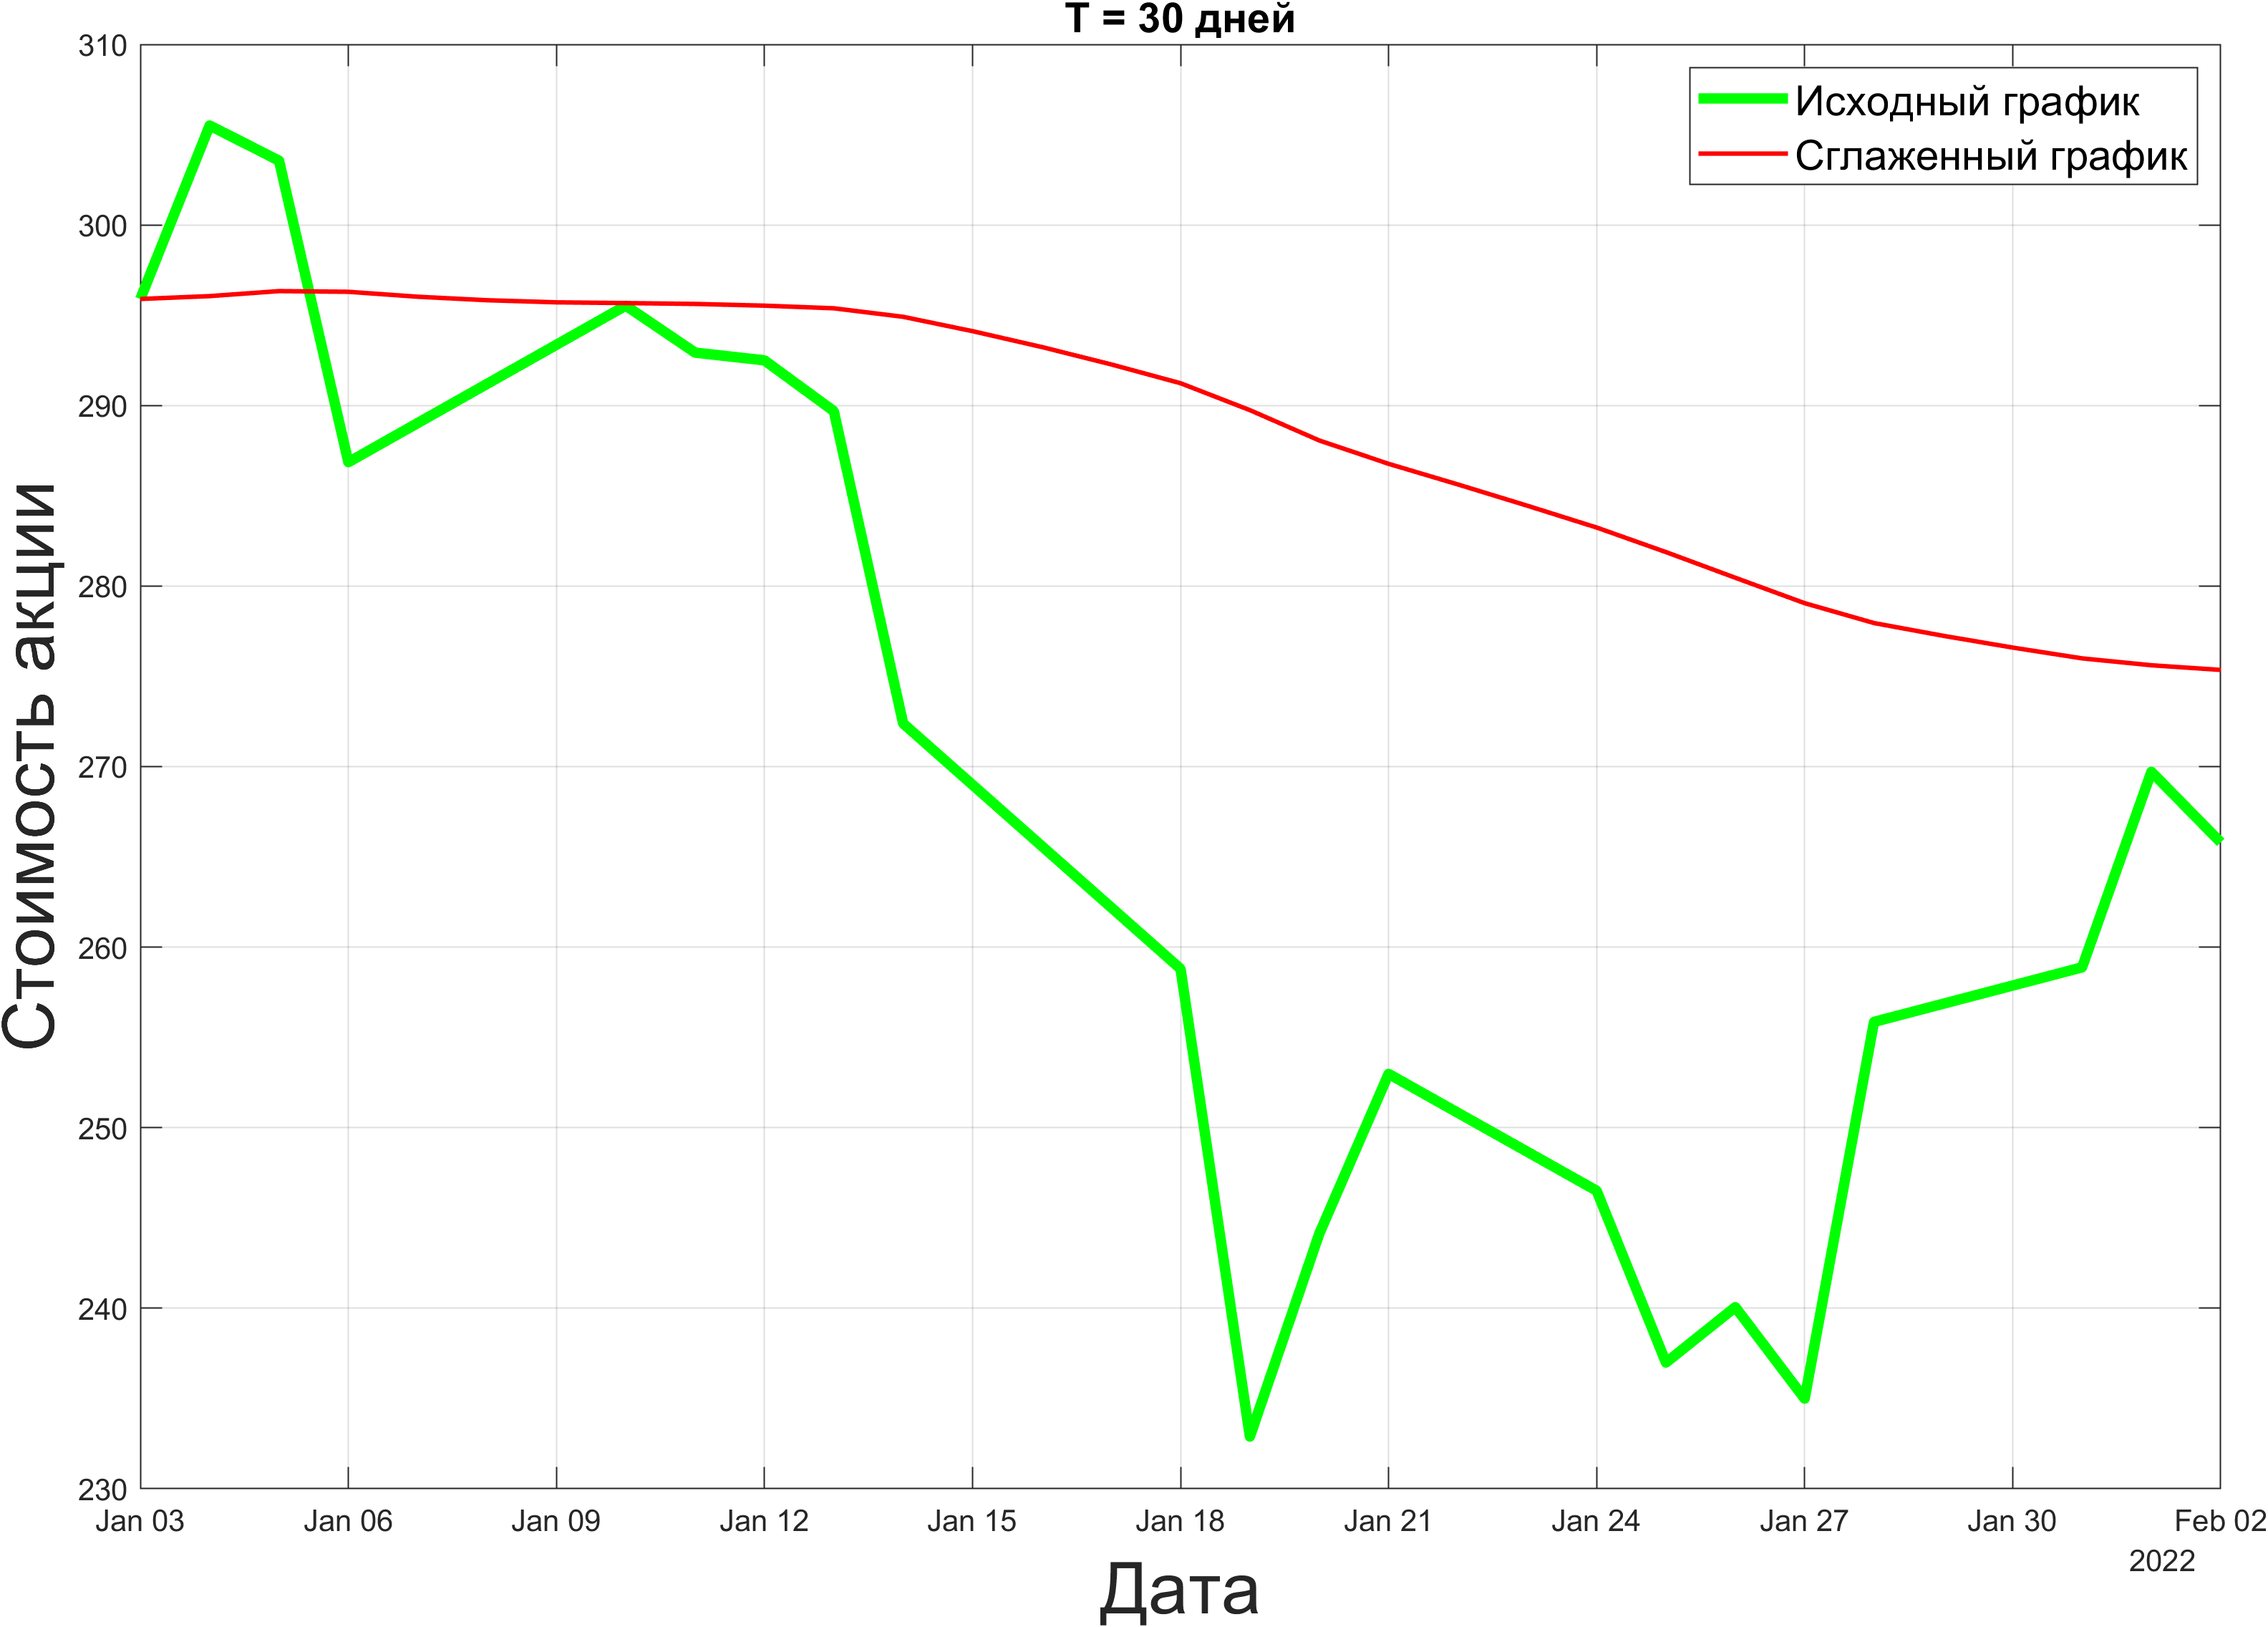
\includegraphics[width=0.90\textwidth, keepaspectratio]{images4/task3_30_2.png}
    \caption{Сглаживание, $T = 30$ дней, период времени $T$}
\end{figure}
\newpage
\begin{figure}[H]
    \centering
    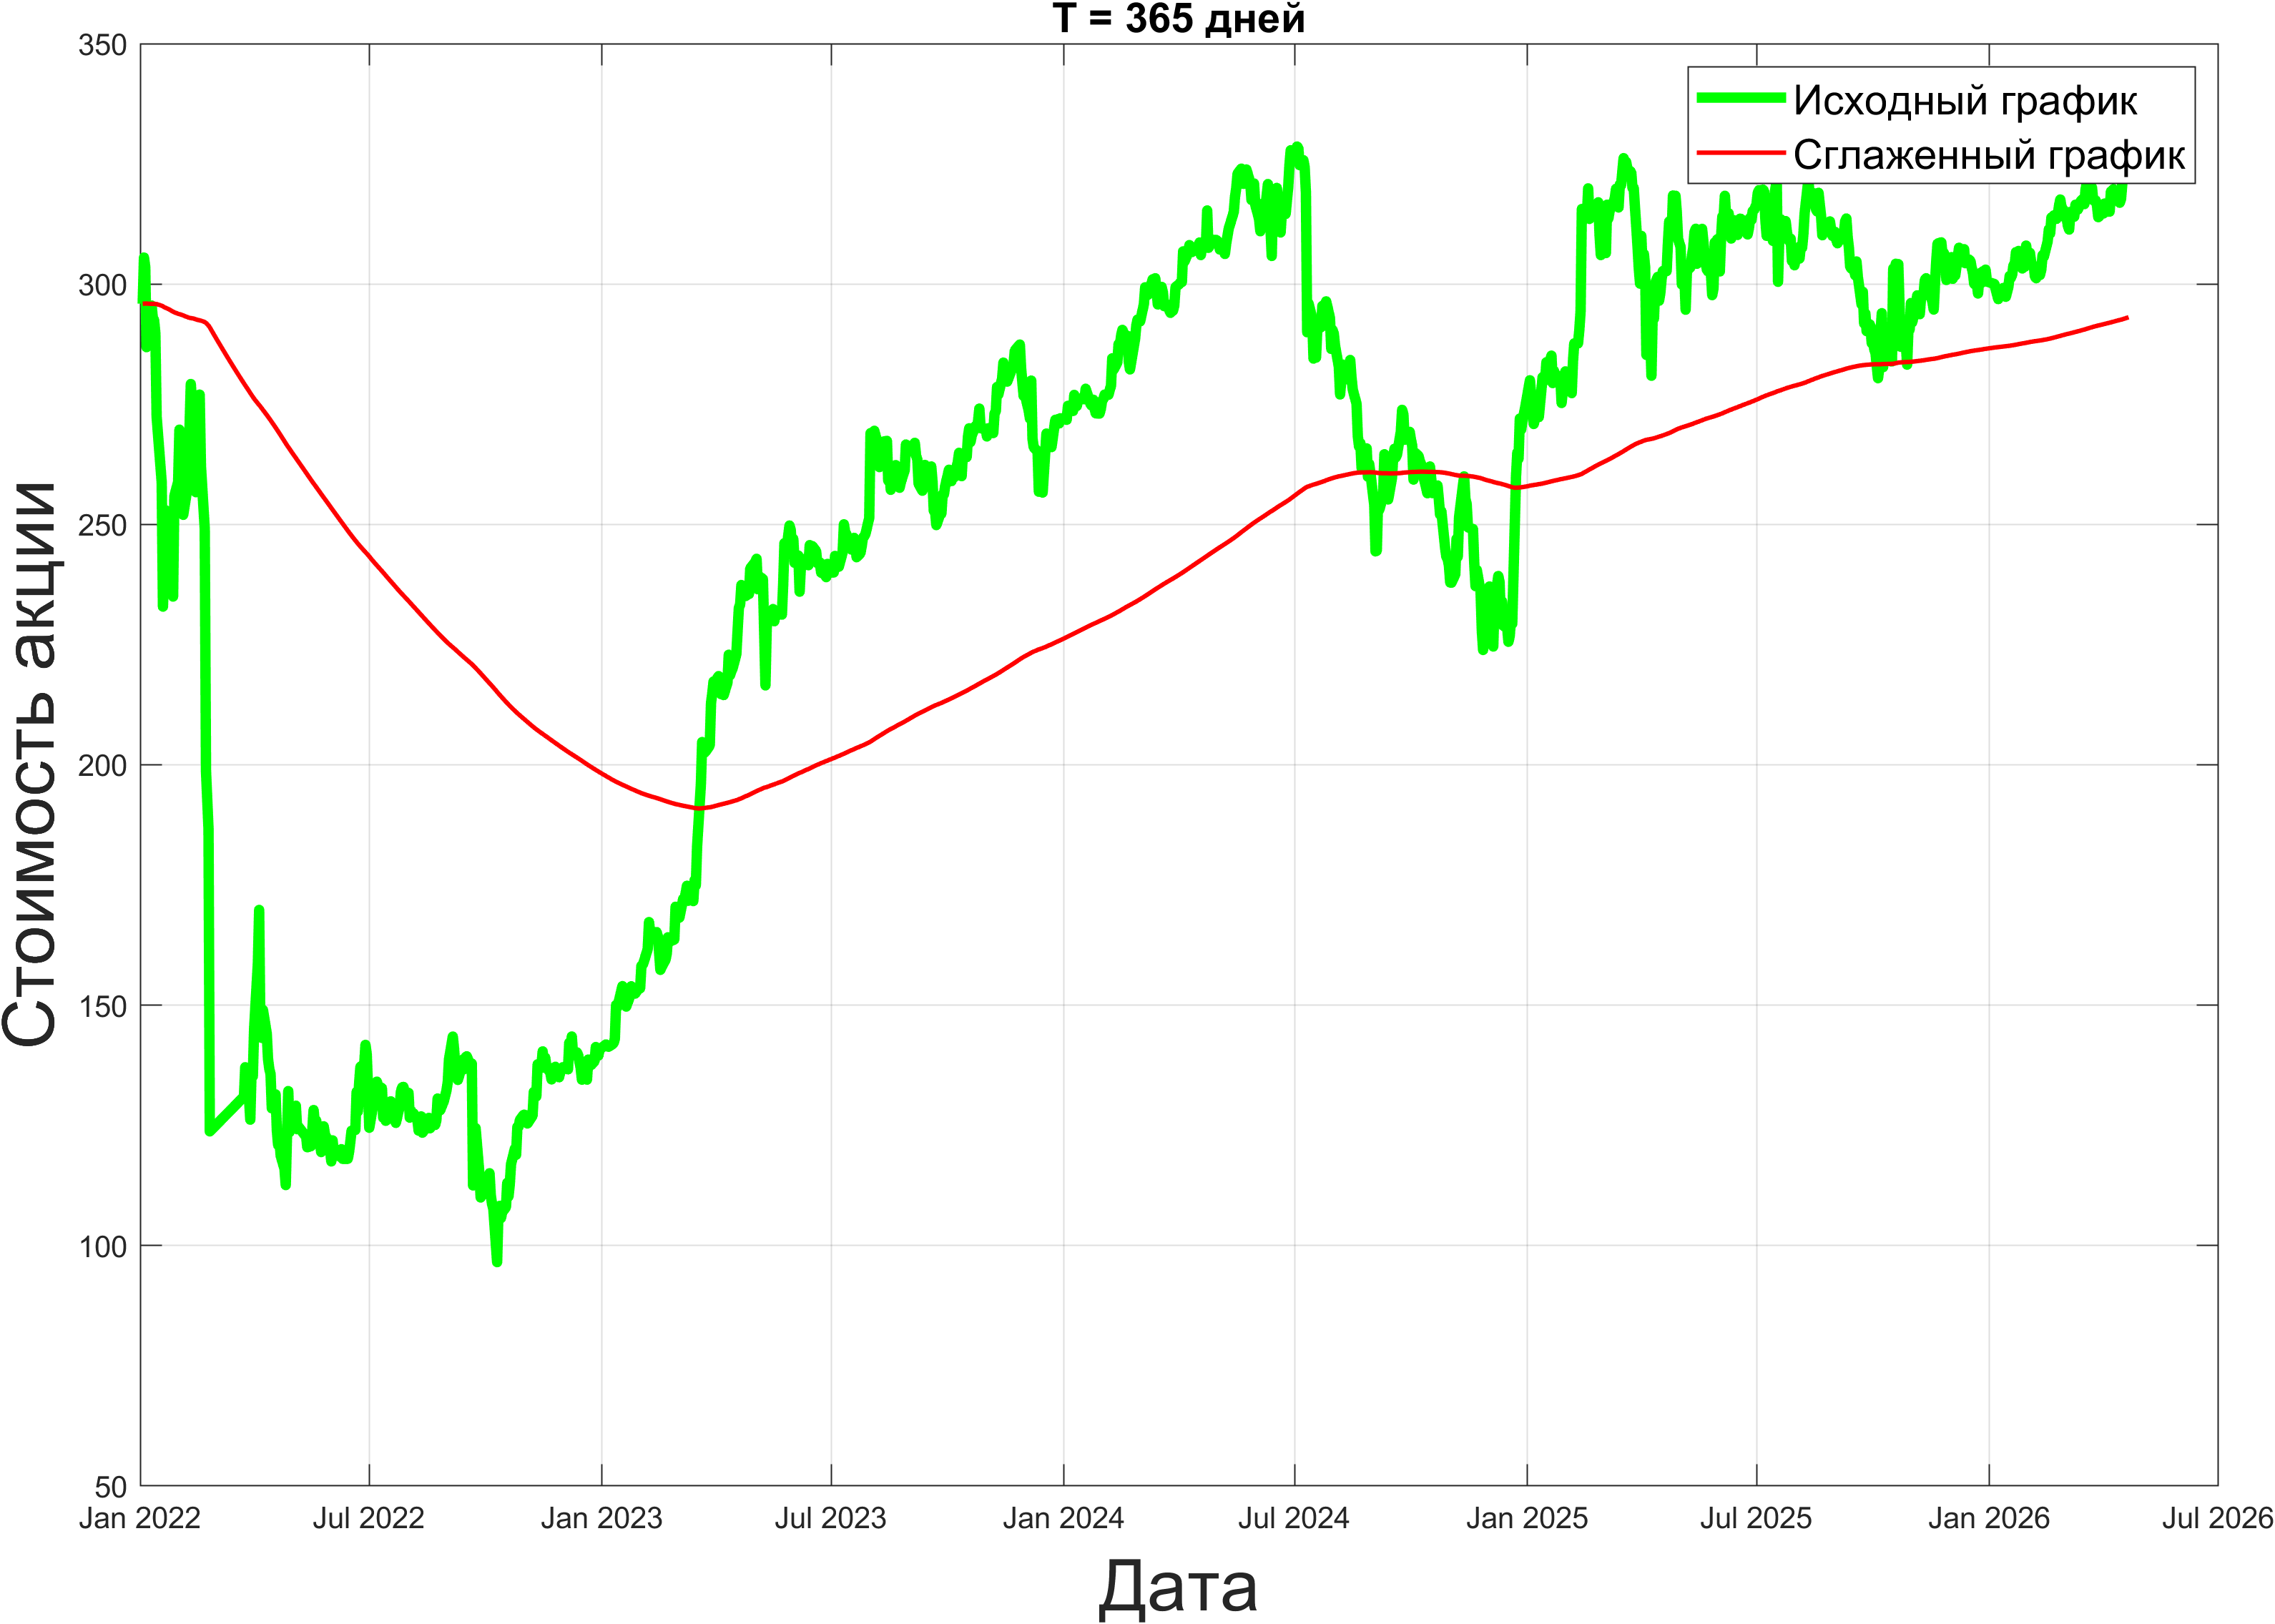
\includegraphics[width=0.90\textwidth, keepaspectratio]{images4/task3_365_1.png}
    \caption{Сглаживание, $T = 365$ дней, все время}
\end{figure}
\begin{figure}[H]
    \centering
    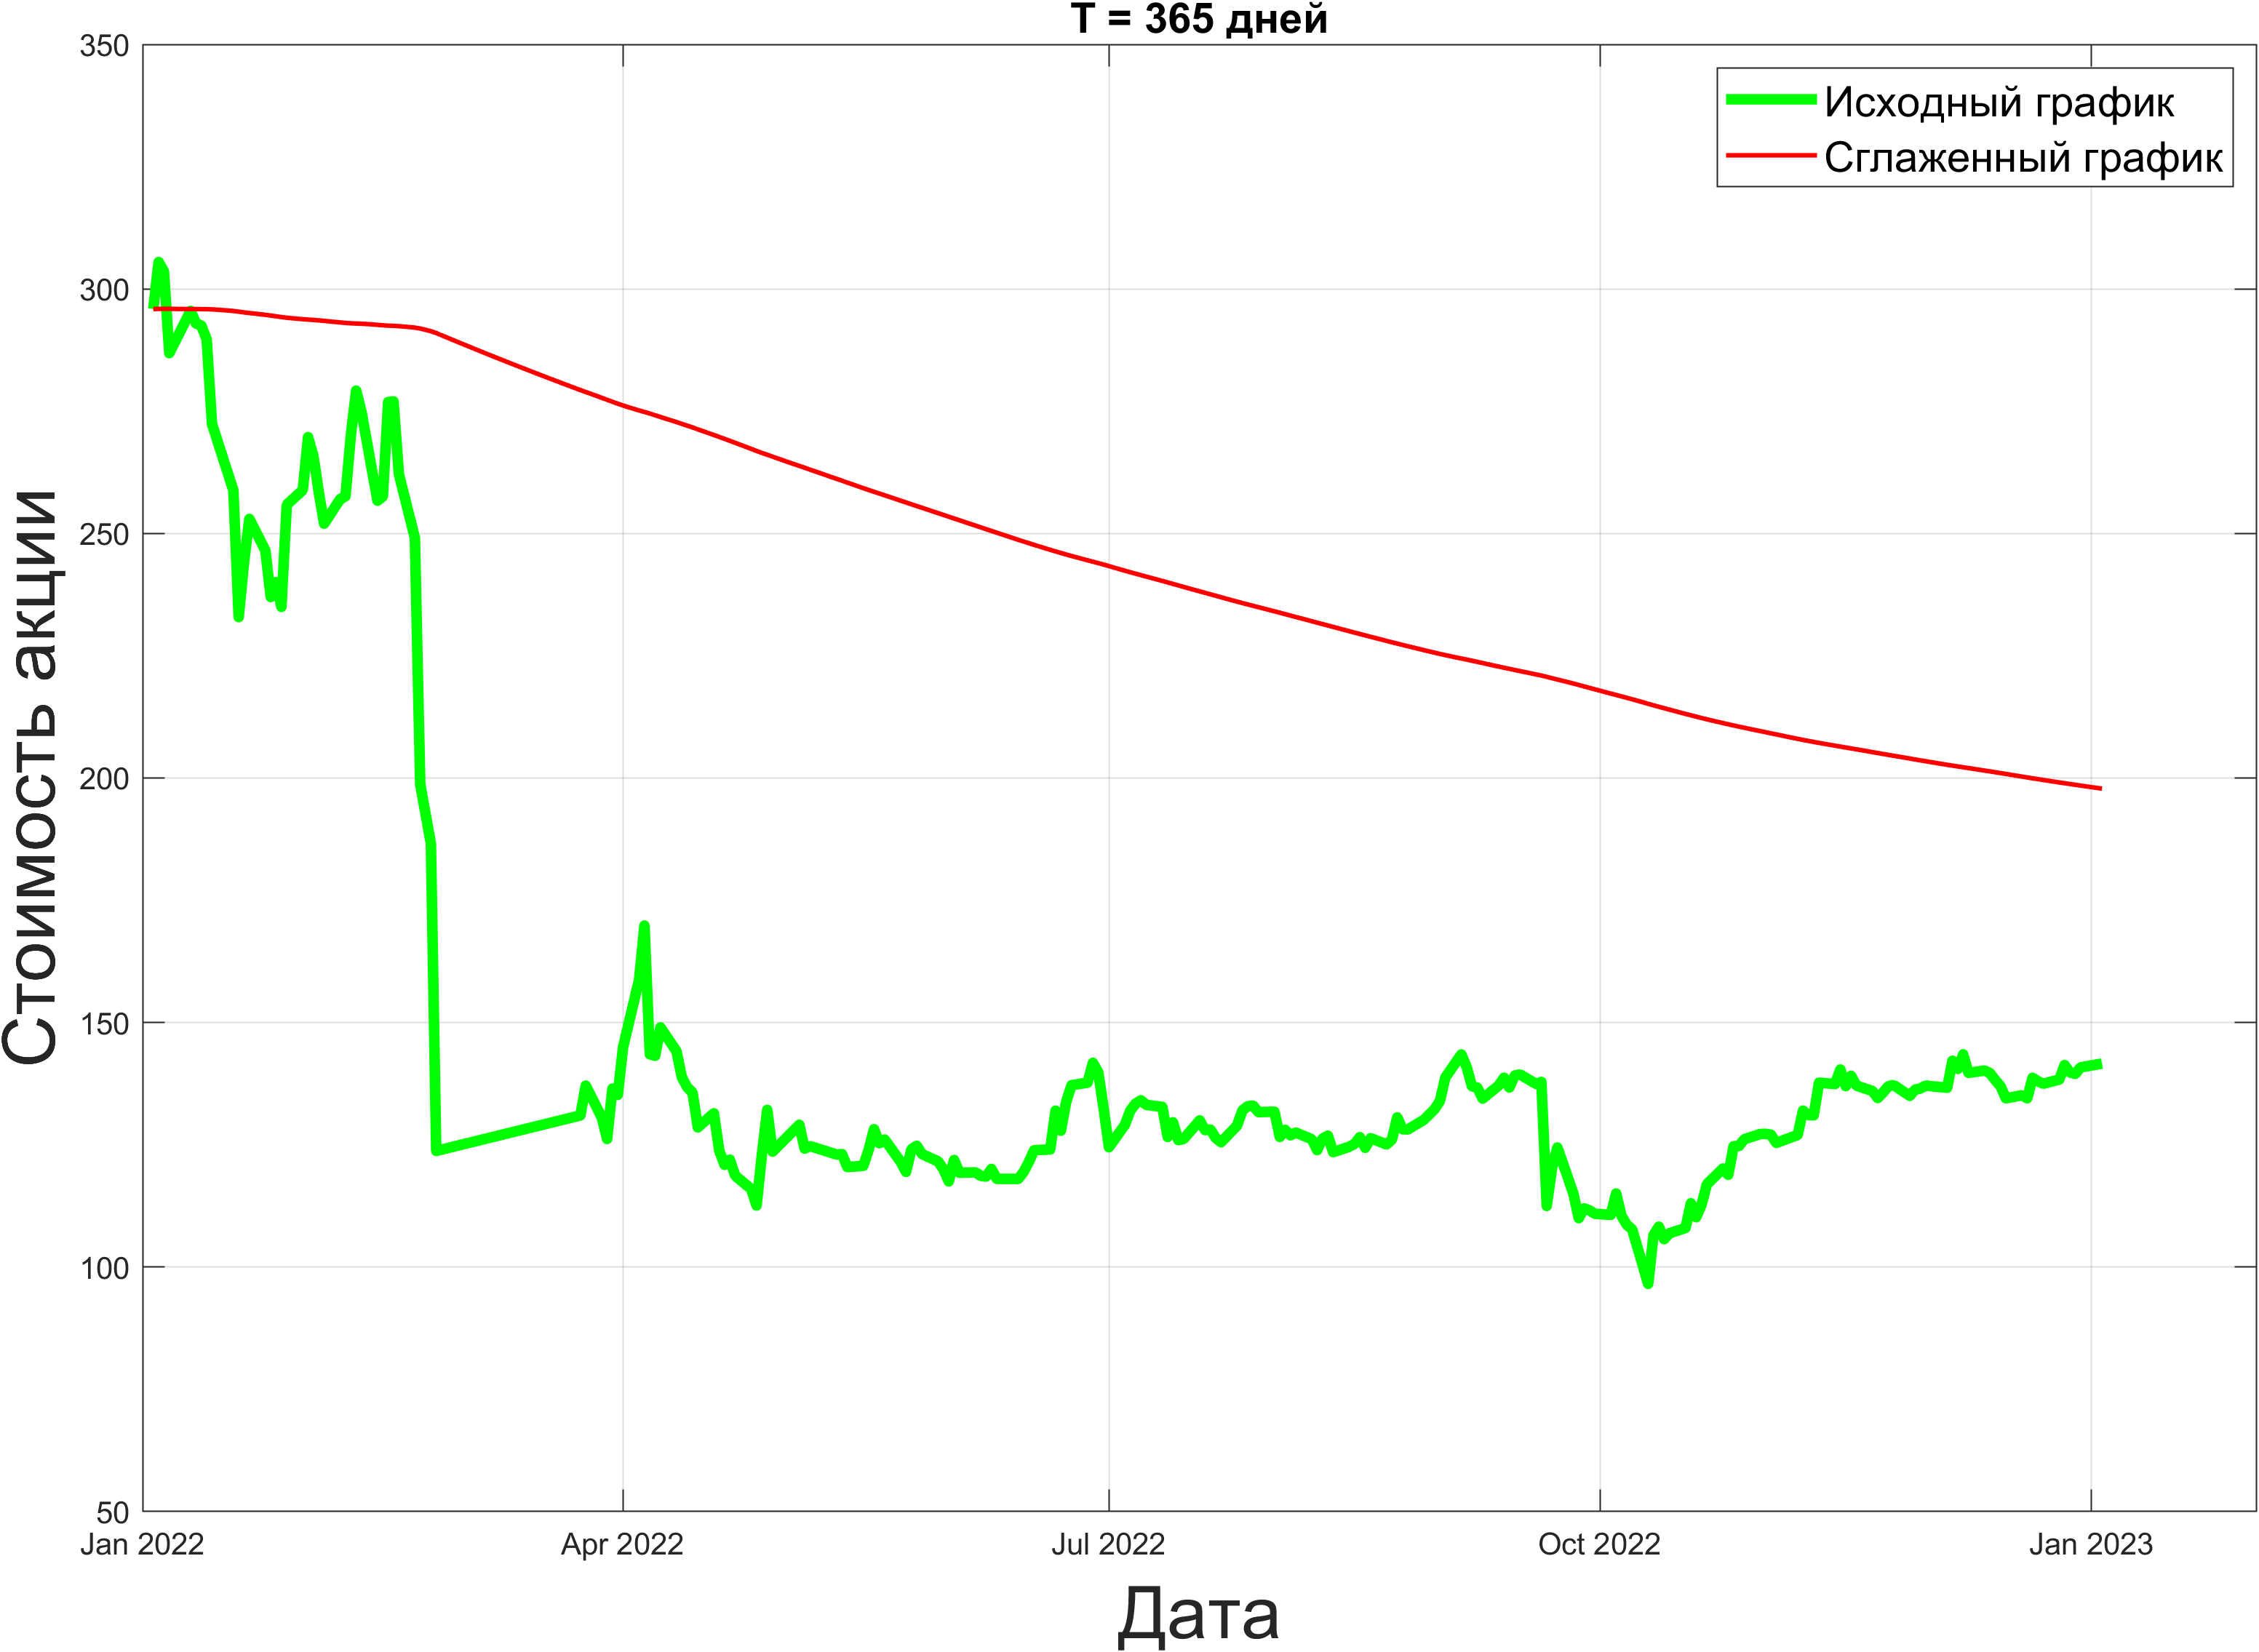
\includegraphics[width=0.90\textwidth, keepaspectratio]{images4/task3_365_2.png}
    \caption{Сглаживание, $T = 365$ дней, период времени $T$}
\end{figure}
\newpage
\subsection{Выводы}
Видим, что чем больше $T$, тем сильнее фильтруются высокие частоты и, соответственно, тем более пологим получается график после фильтрации.
\section{Вывод}
В работе были исследованы линейные динамические фильтры: фильтр низких частот 1 порядка и режекторный полосовой фильтр второго порядка. Исследована зависимость результата фильтрации от коэффициентов соответствующего линейного дифф. уравнения. 
\newline
Для обоих фильтров подтвердилась тождественность функции полученной с помощью фильтрации и функции, полученной с помощью обратного преобразования фурье от произведения частотной передаточной функции и фурье-образа зашумленного сигнала. 
\newline
Также было проведено сглаживание графика акций сбербанка с помощью линейного динамического фильтра низких частот.
\section{Приложения}
\begin{lstlisting}[caption={Код для фильтрации функции в первом пункте}]
width = 800;
height = 600;
resolution = 300;
a = 1;
t1 = 0;
t2 = 2*pi;
N = 500;
b = 0.5;
dt = 0.1;
Fs = 1/dt;
T = N*dt; 
t = (-T/2 : dt : T/2-dt)';

f_Hz = (0:N-1)' * Fs/N; 
omega = 2*pi * f_Hz;

T_arr = [0.1, 0.5, 1.25, 2.0];
a_arr = [1.0, 2.0, 7.5, 10.0];


for i = 1:length(T_arr)
    xi = -1 + 2 * rand(N, 1);
    g = zeros(size(t));
    g((t >= t1 & t <= t2)) = a;
    y = g + b*xi;

    T_c = T_arr(i);
    w = tf(1, [T_c, 1]);
    
    figure;
    [amp, ~, wout] = bode(w);
    amp = squeeze(amp);
    plot(wout, amp, 'LineWidth', 1.5);
    grid on;
    ylim([0 1.1]);
    xlim([0 10]);
    xlabel("w", FontSize=24);
    ylabel("W(iw)",FontSize=24);
    title("АЧХ динамического фильтра при T = " + T_c, FontSize=24);
    legend("АЧХ динамического фильтра T = " + T_c, 'Location', 'northeast', fontsize=18);
    set(gcf, 'Units', 'pixels', 'Position', [100, 100, 1200, 800]);
    exportgraphics(gcf, "filter_ach_T_" + T_c + ".png", 'Resolution', 300);
    
    w_d = c2d(w, dt, 'zoh');
    [H_d, ~] = freqz(w_d.Num{1}, w_d.Den{1}, N, 'whole');
    
    Y = fft(y);
    H_d = H_d(:);  % Явно делаем столбцом
    Y = Y(:);
    y_fil_rev = real(ifft(Y .* H_d));
    
    y_fil = lsim(w, y, t);
    
    y_fur = fftshift(fft(y));
    g_fur = fftshift(fft(g));
    fil_fur = fftshift(fft(y_fil));
    Y_fur_plot = fftshift(Y .* H_d);

    figure;
    plot(t, g, 'LineWidth', 3.5, color="blue");
    hold on;
    plot(t, y, 'LineWidth', 0.5, color="red");
    hold on;
    plot(t, y_fil, 'LineWidth', 3.5, color="green");
    hold off;
    grid on;
    ylim([-0.5 1.5]);
    xlim([-T/2 T/2]);
    xlabel("t", FontSize=24);
    ylabel("y(t)",FontSize=24);
    title("Фильтрация сигнала при T = " + T_c, FontSize=24);
    legend("Оригинал", "Зашумлённая функция", "Фильтрованная функция",  'Location', 'northeast', fontsize=14);
    set(gcf, 'Units', 'pixels', 'Position', [100, 100, 1200, 800]);
    exportgraphics(gcf, "filter_T_" + T_c + ".png", 'Resolution', 300);

    figure;
    plot(t, y_fil, 'LineWidth', 1.25, color="blue");
    hold on;
    plot(t, y_fil_rev, 'LineWidth', 1.25, color="red");
    hold off;
    grid on;
    xlabel("t", FontSize=24);
    ylabel("y(t)",FontSize=24);
    title("Сравнение сигналов при T = " + T_c, FontSize=24);
    legend("lsim (временной)", "ifft (частотный)",  'Location', 'northeast', fontsize=14);
    set(gcf, 'Units', 'pixels', 'Position', [100, 100, 1200, 800]);
    exportgraphics(gcf, "filter_transf_T_" + T_c + ".png", 'Resolution', 300);

    figure;
    plot(omega, abs(y_fur), 'LineWidth', 1.0, color="blue");
    hold on;
    plot(omega, abs(g_fur), 'LineWidth', 0.5, color="red");
    hold on;
    plot(omega, abs(fil_fur), 'LineWidth', 1.0, color="green");
    hold off;
    grid on;
    ylim([-1.5 50.5]);
    xlim([0 63]);
    xlabel("w", FontSize=24);
    ylabel("y(w)",FontSize=24);
    title("Сравнение фурье-образов при T = " + T_c, FontSize=24);
    legend("Образ зашумлённой функции", "Образ исходной функции", "Образ фильтрованной функции",  'Location', 'northeast', fontsize=14);
    set(gcf, 'Units', 'pixels', 'Position', [100, 100, 1200, 800]);
    exportgraphics(gcf, "fur_imgs_g_T_" + T_c + ".png", 'Resolution', 300);

    figure;
    plot(omega, abs(Y_fur_plot), 'LineWidth', 0.5, color="red");
    hold on;
    plot(omega, abs(fil_fur), 'LineWidth', 1.0, color="blue");
    hold off;
    grid on;
    ylim([-1.5 50.5]);
    xlim([0 63]);
    xlabel("w", FontSize=24);
    ylabel("y(w)",FontSize=24);
    title("Сравнение фурье-образов при T = " + T_c, FontSize=24);
    legend("Умножение на передаточную функцию", "Образ фильтрованной функции",  'Location', 'northeast', fontsize=14);
    set(gcf, 'Units', 'pixels', 'Position', [100, 100, 1200, 800]);
    exportgraphics(gcf, "fur_imgs_w_T_" + T_c + ".png", 'Resolution', 300);

    a_c = a_arr(i);
    xi = -1 + 2 * rand(N, 1);
    
    g = zeros(size(t));
    g((t >= t1 & t <= t2)) = a_c;
    y = g + b*xi;

    w = tf(1, [1.1, 1]);
    
    figure;
    [amp, ~, wout] = bode(w);
    amp = squeeze(amp);
    plot(wout, amp, 'LineWidth', 1.5);
    grid on;
    ylim([0 1]);
    xlim([0 10]);
    xlabel("w", FontSize=24);
    ylabel("W(iw)",FontSize=24);
    title("АЧХ динамического фильтра при a = " + a_c + ", T = 1.25", FontSize=24);
    legend("АЧХ динамического фильтра a = " + a_c, 'Location', 'northeast', fontsize=14);
    set(gcf, 'Units', 'pixels', 'Position', [100, 100, 1200, 800]);
    exportgraphics(gcf, "filter_ach_a_" + a_c + ".png", 'Resolution', 300);

    w_d = c2d(w, dt, 'zoh');
    [H_d, ~] = freqz(w_d.Num{1}, w_d.Den{1}, N, 'whole');
    
    Y = fft(y);
    H_d = H_d(:);
    Y = Y(:);
    y_fil_rev = real(ifft(Y .* H_d));
    
    y_fil = lsim(w, y, t);
    
    y_fur = fftshift(fft(y));
    g_fur = fftshift(fft(g));
    fil_fur = fftshift(fft(y_fil));
    Y_fur_plot = fftshift(Y .* H_d);

    figure;
    plot(t, y_fil, 'LineWidth', 1.0, color="blue");
    hold on;
    plot(t, y_fil_rev, 'LineWidth', 1.0, color="red");
    hold off;
    grid on;
    xlabel("t", FontSize=24);
    ylabel("y(t)",FontSize=24);
    title("Сравнение сигналов при a = " + a_c + ", T = 1.25", FontSize=24);
    legend("lsim (временной)", "ifft (частотный)",  'Location', 'northeast', fontsize=14);
    set(gcf, 'Units', 'pixels', 'Position', [100, 100, 1200, 800]);
    exportgraphics(gcf, "filter_transf_a_" + a_c + ".png", 'Resolution', 300);
    
    figure;
    plot(t, g, 'LineWidth', 3.5, color="blue");
    hold on;
    plot(t, y, 'LineWidth', 0.5, color="red");
    hold on;
    plot(t, y_fil, 'LineWidth', 3.5, color="green");
    hold off;
    grid on;
    ylim([-0.5 a_c+1]);
    xlim([-T/2 T/2]);
    xlabel("t", FontSize=24);
    ylabel("y(t)",FontSize=24);
    title("Фильтрация сигнала при a = " + a_c + ", T = 1.25", FontSize=24);
    legend("Оригинал", "Зашумлённая функция", "Фильтрованная функция",  'Location', 'northeast', fontsize=14);
    set(gcf, 'Units', 'pixels', 'Position', [100, 100, 1200, 800]);
    exportgraphics(gcf, "filter_a_" + a_c + ".png", 'Resolution', 300);
    
    figure;
    plot(omega, abs(y_fur), 'LineWidth', 1.0, color="blue");
    hold on;
    plot(omega, abs(g_fur), 'LineWidth', 0.5, color="red");
    hold on;
    plot(omega, abs(fil_fur), 'LineWidth', 1.0, color="green");
    hold off;
    grid on;
    ylim([-1.5 50.5]);
    xlim([0 63]);
    xlabel("w", FontSize=24);
    ylabel("y(w)",FontSize=24);
    title("Сравнение фурье-образов при a = " + a_c + ", T = 1.25", FontSize=24);
    legend("Образ зашумлённой функции", "Образ исходной функции", "Образ фильтрованной функции",  'Location', 'northeast', fontsize=14);
    set(gcf, 'Units', 'pixels', 'Position', [100, 100, 1200, 800]);
    exportgraphics(gcf, "fur_imgs_g_a_" + a_c + ".png", 'Resolution', 300);

    figure;
    plot(omega, abs(Y_fur_plot), 'LineWidth', 0.5, color="red");
    hold on;
    plot(omega, abs(fil_fur), 'LineWidth', 1.0, color="blue");
    hold off;
    grid on;
    ylim([-1.5 50.5]);
    xlim([0 63]);
    xlabel("w", FontSize=24);
    ylabel("y(w)",FontSize=24);
    title("Сравнение фурье-образов при a = " + a_c + ", T = 1.25", FontSize=24);
    legend("Умножение на передаточную функцию", "Образ фильтрованной функции",  'Location', 'northeast', fontsize=14);
    set(gcf, 'Units', 'pixels', 'Position', [100, 100, 1200, 800]);
    exportgraphics(gcf, "fur_imgs_w_a_" + a_c + ".png", 'Resolution', 300);
end
\end{lstlisting}
\begin{lstlisting}[caption={Код для фильтрации функции во втором пункте}]
width = 800;
height = 600;
resolution = 300;
a = 1;
t1 = 0;
t2 = 2*pi;
N = 500;
b = 0;
c = 0.5;
d = 10;
dt = 0.1;
Fs = 1/dt;
T = N*dt; 
t = (-T/2 : dt : T/2-dt)';

f_Hz = (0:N-1)' * Fs/N; 
omega = 2*pi * f_Hz;

%T_arr = [0.1, 0.5, 1.25, 2.0];
a1 = 0;
a2 = 25;
b1 = 25;
b2 = 25;
%a_arr = [1.0, 2.0, 7.5, 10.0];


xi = -1 + 2 * rand(N, 1);
g = zeros(size(t));
g((t >= t1 & t <= t2)) = a;
y = g + b*xi + c * sin(d * t);

w = tf([1, a1, a2], [1, b1, b2]);
    
figure;
[amp, ~, wout] = bode(w);
amp = squeeze(amp);
plot(wout, amp, 'LineWidth', 1.5);
grid on;
ylim([0 1.1]);
xlim([0 10]);
xlabel("w", FontSize=24);
ylabel("W(iw)",FontSize=24);
title("АЧХ динамического фильтра при b1 = " + b1, FontSize=24);
legend("АЧХ динамического фильтра b1 = " + b1, 'Location', 'northeast', fontsize=18);
set(gcf, 'Units', 'pixels', 'Position', [100, 100, 1200, 800]);
exportgraphics(gcf, "filter_ach_b1_" + b1 + ".png", 'Resolution', 300);
    
w_d = c2d(w, dt, 'foh');
[H_d, ~] = freqz(w_d.Num{1}, w_d.Den{1}, N, 'whole');
    
Y = fft(y);
H_d = H_d(:);  % Явно делаем столбцом
Y = Y(:);
y_fil_rev = real(ifft(Y .* H_d));
    
y_fil = lsim(w, y, t);
    
y_fur = fftshift(fft(y));
g_fur = fftshift(fft(g));
fil_fur = fftshift(fft(y_fil));
Y_fur_plot = fftshift(Y .* H_d);

figure;
plot(t, g, 'LineWidth', 3.5, color="blue");
hold on;
plot(t, y, 'LineWidth', 0.5, color="red");
hold on;
plot(t, y_fil, 'LineWidth', 3.5, color="green");
hold off;
grid on;
ylim([-0.5 1.5]);
xlim([-T/2 T/2]);
xlabel("t", FontSize=24);
ylabel("y(t)",FontSize=24);
title("Фильтрация сигнала при b1 = " + b1, FontSize=24);
legend("Оригинал", "Зашумлённая функция", "Фильтрованная функция",  'Location', 'northeast', fontsize=14);
set(gcf, 'Units', 'pixels', 'Position', [100, 100, 1200, 800]);
exportgraphics(gcf, "filter_b1_" + b1 + ".png", 'Resolution', 300);

figure;
plot(t, y_fil, 'LineWidth', 1.25, color="blue");
hold on;
plot(t, y_fil_rev, 'LineWidth', 1.25, color="red");
hold off;
grid on;
xlabel("t", FontSize=24);
ylabel("y(t)",FontSize=24);
title("Сравнение сигналов при b1 = " + b1, FontSize=24);
legend("lsim (временной)", "ifft (частотный)",  'Location', 'northeast', fontsize=14);
set(gcf, 'Units', 'pixels', 'Position', [100, 100, 1200, 800]);
exportgraphics(gcf, "filter_transf_b1_" + b1 + ".png", 'Resolution', 300);

figure;
plot(omega, abs(y_fur), 'LineWidth', 1.0, color="blue");
hold on;
plot(omega, abs(g_fur), 'LineWidth', 0.5, color="red");
hold on;
plot(omega, abs(fil_fur), 'LineWidth', 1.0, color="green");
hold off;
grid on;
ylim([-1.5 50.5]);
xlim([0 63]);
xlabel("w", FontSize=24);
ylabel("y(w)",FontSize=24);
title("Сравнение фурье-образов при b1 = " + b1, FontSize=24);
legend("Образ зашумлённой функции", "Образ исходной функции", "Образ фильтрованной функции",  'Location', 'northeast', fontsize=14);
set(gcf, 'Units', 'pixels', 'Position', [100, 100, 1200, 800]);
exportgraphics(gcf, "fur_imgs_g_b1_" + b1 + ".png", 'Resolution', 300);

figure;
plot(omega, abs(Y_fur_plot), 'LineWidth', 0.5, color="red");
hold on;
plot(omega, abs(fil_fur), 'LineWidth', 1.0, color="blue");
hold off;
grid on;
ylim([-1.5 50.5]);
xlim([0 63]);
xlabel("w", FontSize=24);
ylabel("y(w)",FontSize=24);
title("Сравнение фурье-образов при b1 = " + b1, FontSize=24);
legend("Умножение на передаточную функцию", "Образ фильтрованной функции",  'Location', 'northeast', fontsize=14);
set(gcf, 'Units', 'pixels', 'Position', [100, 100, 1200, 800]);
exportgraphics(gcf, "fur_imgs_w_b1_" + b1 + ".png", 'Resolution', 300);
\end{lstlisting}
\begin{lstlisting}[caption={Код для фильтрации функции в третьем пункте}]
tablica = readtable("SBER_220101_260421.csv");
stoimost = table2array(tablica(:, 5));
dates = table2array(tablica(:, 3));
days = zeros(size(dates));
months = zeros(size(dates));
years = zeros(size(dates));
Datestart = datetime(2022, 1, 3);
Datefinish = datetime(2026, 4, 21);
datesfull = Datestart:Datefinish;
for i = 1:length(dates)
    day = mod(dates(i), 100);
    month = mod(dates(i), 10000) - day;
    year = (dates(i) - day - month) / 10000;
    month = month / 100;
    days(i) = day;
    months(i) = month;
    years(i) = year;
end
dates_new = datetime(years, months, days);
stoimostfull = zeros(size(datesfull));
c = 1;
for i = 1:length(datesfull)
    if datesfull(i) == dates_new(c)
        stoimostfull(i) = stoimost(c);
        c = c + 1;
    else
        a = datenum(dates_new(c)) - datenum(dates_new(c - 1));
        b = datenum(datesfull(i)) - datenum(dates_new(c - 1));
        otn = b / a;
        stoimostfull(i) = stoimost(c - 1) + (stoimost(c) - stoimost(c - 1)) * otn;
    end
end
T = 365;
w1 = tf(1, [T, 1]);
massiv = zeros(size(datesfull));
for i = 1:length(datesfull)
    %massiv(i) = datenum(dates_new(i)) - datenum(dates_new(1));
    massiv(i) = i - 1;
end
stoimostfullnorm = stoimostfull - stoimostfull(1);
stoimostgladnorm = lsim(w1, stoimostfullnorm, massiv);
stoimostglad = stoimostgladnorm + stoimostfull(1);
plot(datesfull, stoimostfull, 'LineWidth', 3.5, color="green");
hold on;
plot(datesfull, stoimostglad, 'LineWidth', 1.5, color="red");
hold off;
grid on;
xlabel("Дата", FontSize=24);
ylabel("Стоимость акции",FontSize=24);
title("T = 365 дней", FontSize=14);
legend("Исходный график", "Сглаженный график",  'Location', 'northeast', fontsize=14);
set(gcf, 'Units', 'pixels', 'Position', [100, 100, 1200, 800]);
exportgraphics(gcf, "task3_" + T + "_1.png", 'Resolution', 300);

plot(datesfull(1:T + 1), stoimostfull(1:T + 1), 'LineWidth', 3.5, color="green");
hold on;
plot(datesfull(1:T + 1), stoimostglad(1:T + 1), 'LineWidth', 1.5, color="red");
hold off;
grid on;
xlabel("Дата", FontSize=24);
ylabel("Стоимость акции",FontSize=24);
title("T = 365 дней", FontSize=14);
legend("Исходный график", "Сглаженный график",  'Location', 'northeast', fontsize=14);
set(gcf, 'Units', 'pixels', 'Position', [100, 100, 1200, 800]);
exportgraphics(gcf, "task3_" + T + "_2.png", 'Resolution', 300);
\end{lstlisting}
\end{document}
